\documentclass[titlepage,12pt,twoside,a4paper]{report}

\usepackage[utf8]{inputenc}
\usepackage{kantlipsum}
\usepackage{capt-of}
\usepackage[english]{babel}
\usepackage{csquotes}
\usepackage{pdfcolmk}
\usepackage{graphicx}
\usepackage[hyphens]{url}
\def\UrlBreaks{\do\/\do-}
\usepackage{breakurl}
%\usepackage[breaklinks]{hyperref}
\usepackage{epstopdf}
\usepackage{adjustbox}
\usepackage{pdflscape}
\usepackage{amsmath,amssymb}
\usepackage{bm}
\usepackage{amstext}
\usepackage{amsthm}
\usepackage{rotating}
\usepackage{enumerate}
\usepackage{epigraph}
\usepackage[backref=true,backend=bibtex,style=chem-acs,natbib=true,doi=true,isbn=false,url=true,arxiv=false]{biblatex}
\DefineBibliographyStrings{english}{%
	  backrefpage = {page},% originally "cited on page"
	    backrefpages = {pages},% originally "cited on pages"
	}
%\renewcommand*{\backref}[1]{}
%
%	\renewcommand*{\backrefalt}[4]{%
%	\ifcase #1%
%	\or [Page~#2]%
%	\else [Pages~#2]%
%	\fi%
%}
\addbibresource{./library}


\usepackage[backref=pages,colorlinks=true,pdfstartview=FitV,breaklinks=true]{hyperref}



\usepackage{multirow}
\usepackage[usenames,dvipsnames]{color}
\usepackage{verbatim}
\usepackage{float}
\usepackage{afterpage}
\usepackage{longtable}
\usepackage{tabularx}
%\usepackage[table] {xcolor}
\usepackage[table,svgnames] {xcolor}

\hypersetup{
    colorlinks=true,
    citecolor=red,
    filecolor=black,
    linkcolor=blue,
    urlcolor=blue
}
\usepackage[font=small,labelfont=bf]{caption}
\DeclareCaptionLabelFormat{adja-page}{\hrulefill\\#1 #2 \emph{(previous page)}}
%\captionsetup{justification=raggedright,singlelinecheck=false,format=hang}
\usepackage{pdfpages}
\usepackage[utf8]{inputenc}
\usepackage[english]{babel}
\usepackage{parskip,array,booktabs}
\raggedbottom
\DeclareUnicodeCharacter{2212}{-}
\DeclareUnicodeCharacter{0301}{\'{e}}
\usepackage{listings}
\usepackage{color}
\usepackage{appendix}
\usepackage{blindtext}
\usepackage{tikz}

%%%%%%%%%%%%%%%%%%%%%%%
%% PAGE SETUP        %%
%%%%%%%%%%%%%%%%%%%%%%%
\usepackage{geometry}
\geometry{paper=a4paper,            % scientific thesis standard
            left=3cm,
            right=2.5cm,
            top=3cm,
            bottom=3cm,
 }
\setlength{\headheight}{27.2pt}
\bibliography{library.bib}

\usepackage{fancyhdr}
\fancyhead{}
\fancyhead[LO]{\slshape \rightmark}
\fancyhead[RO,LE]{\textbf{\thepage}}
\fancyhead[RE]{\slshape \leftmark}
\fancyfoot{}
\pagestyle{fancy}

\makeatletter
\makeatother

\def\blankpage{%
      \clearpage%
      \thispagestyle{empty}%
      \addtocounter{page}{-1}%
      \null%
      \clearpage}

%%%%%%%%%%%%%%%%%%%%%%%
%% NEW COMMANDS      %%
%%%%%%%%%%%%%%%%%%%%%%%
\renewcommand{\chaptermark}[1]{\markboth{\chaptername \ \thechapter \ \ #1}{}}
\renewcommand{\sectionmark}[1]{\markright{\thesection \ \ #1}}
\renewcommand{\eqref}[1]{\textup{\color{cyan} {\normalfont(\ref{#1}}\normalfont)}}
\newcommand{\figref}[1]{\hyperref[#1]{Fig.~\ref*{#1}}}
\newcommand{\figrefi}[2]{\hyperref[#1]{Fig.~\ref*{#1}~#2}}
\newcommand{\figrefs}[1]{\hyperref[#1]{Figs.~\ref*{#1}}}
\newcommand{\figrefn}[2]{\hyperref[#1]{Figs.~\ref*{#1}~#2}}
\newcommand{\figrefni}[2]{\hyperref[#1]{Figs.~\ref*{#1}--#2}}
\newcommand{\tabref}[1]{\hyperref[#1]{Table~\ref*{#1}}}
\newcommand{\tabrefn}[1]{\hyperref[#1]{Tables~\ref*{#1}}}
\newcommand{\secref}[1]{\hyperref[#1]{Section~\ref*{#1}}}
\newcommand{\appref}[1]{\hyperref[#1]{Appendix~\ref*{#1}}}
\newcommand{\chapref}[1]{\hyperref[#1]{Chapter~\ref*{#1}}}

\newcommand{\chapquote}[3]{\begin{quotation}\textit{#1}\end{quotation} \begin{flushright}#2\end{flushright}}


\newcommand{\angs}{\textup{\AA}}
\newcommand{\Rmin}{$R_{\text{min}}$}
\newcommand{\spring}{kcal/mol/\AA{}\textsuperscript{2}}
\newcommand{\prim}{\textsuperscript{$\prime$}}
\newcommand{\dprim}{\textsuperscript{$\prime\prime$}}
\newcommand{\Na}{Na$^+$}
\newcommand{\K}{K$^+$}
\newcommand{\Hi}{H$^+$}
\newcommand{\Cl}{Cl$^-$}
\newcommand{\Ca}{Ca$^{2+}$}
\newcommand{\Tl}{Tl$^+$}
\newcommand{\GltPh}{Glt$_\text{Ph}$}
\newcommand{\GltTk}{Glt$_\text{Tk}$}
\newcommand{\pka}{p\textit{K}\textsubscript{a}}
\newcommand{\kT}{k_{\text{B}}T}

%\includeonly{./13-S945L}
%\includeonly{./14-Opening}
\includeonly{./15-Conclusions}

\begin{document}
%%%%%%%%%%%%%%%%%%%%%%%
%% PREAMBLE TEXT     %%
%%%%%%%%%%%%%%%%%%%%%%%
\pagenumbering{roman}

\begin{titlepage}

\begin{center}

\vspace*{0.1in}

\begin{LARGE}
Computer Modelling the Root Cause of  \\ 
\end{LARGE}
\vspace*{0.1in}
\begin{LARGE}
Cystic Fibrosis
\end{LARGE}
\begin{large} \\
\vspace{0.1in}
by Miro Alexander Astore

%\vspace{0.1in}
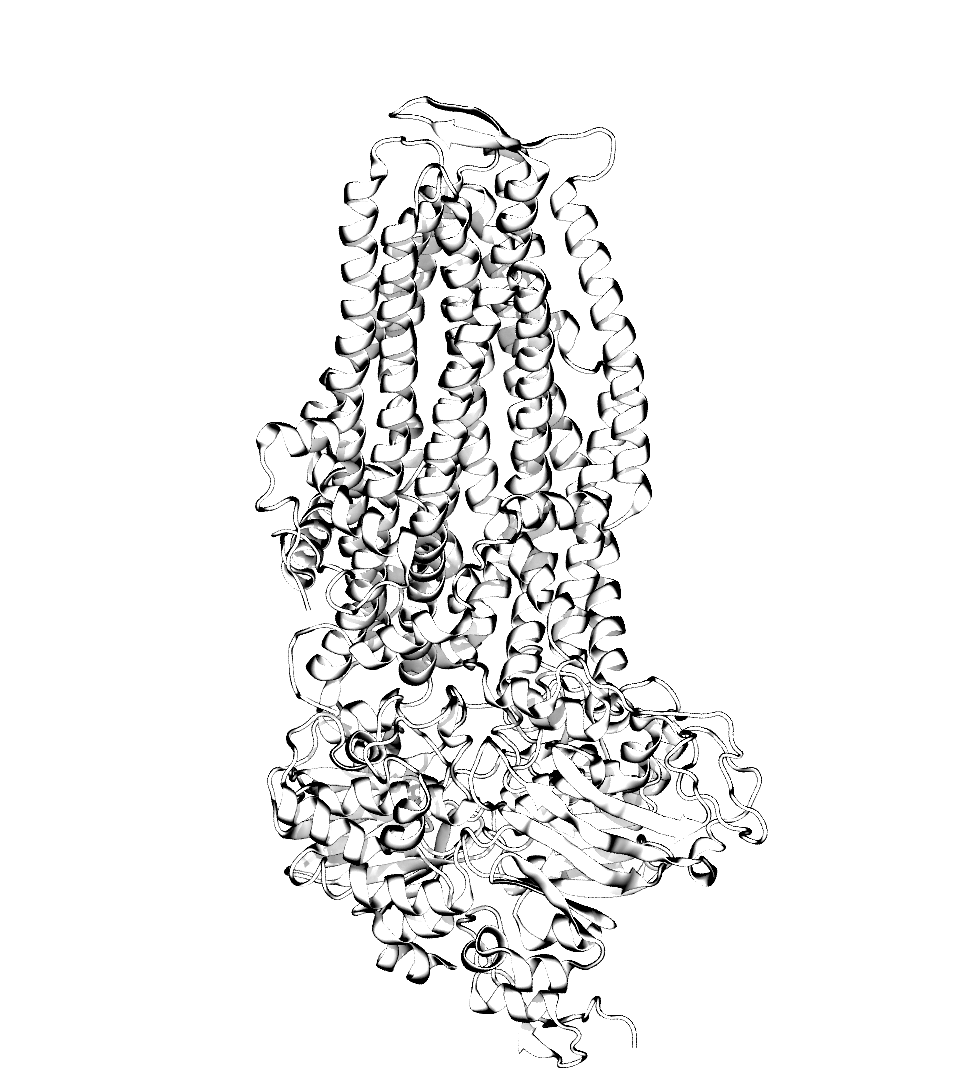
\includegraphics[width=0.8\textwidth]{figures/skeleton_bw.png}
%\vspace{0.1in}
%TO\\
%\vspace{0.1in}
%THE
%{\Large F}ACULTY OF {\Large S}CIENCE\\
\vspace{-0.05in}

\textit{A thesis submitted in fulfilment of the}\\
\textit{requirements for the degree of}

%IN PARTIAL FULFILMENT OF THE REQUIREMENTS\\
%FOR THE DEGREE OF \\
%{\Large D}OCTOR OF {\Large P}HILOSOPHY\\
%IN THE SUBJECT OF \\
%{\Large B}IOPHYSICS\\
\vspace{0.1in}

%\begin{large}
Doctor of Philosophy
%\end{large}

\vspace{0.1in}

%\begin{large}
The School of Physics\\
Faculty of Science\\
The University of Sydney\\
2022
%\vspace{0.05in}
%\end{large}

%\vspace{0.05in}
\end{large}

\end{center}
\end{titlepage}

%=======================================================================================%
\newpage
\begin{center}
Declaration of Original contribution

\vspace{0.5in}

of the dissertation submitted by

\vspace{0.25in}

Miro Alexander Astore

\end{center}

\vspace{0.5in}

\noindent This is to certify that to the best of my knowledge, the content of this 
thesis is my own work. This thesis has not been submitted for any degree or other 
purposes.

\noindent I certify that the intellectual content of this thesis is the product of 
my own work and that all the assistance received in preparing this thesis and sources 
have been acknowledged.

\vspace{1in}

% \begin{tikzpicture}[remember picture,overlay]
%     \node[xshift=4cm,yshift=-14.0cm,anchor=north west] at (current page.north west){%
%     \includegraphics[width=35mm]{Figures/signature-JS.jpg}};
% \end{tikzpicture}

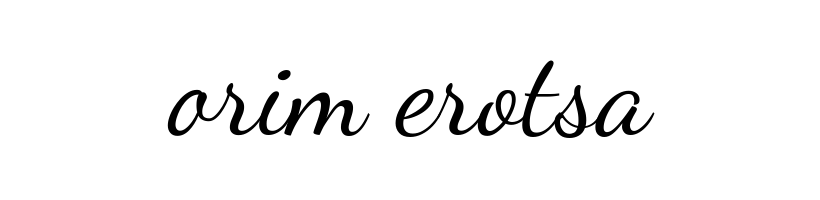
\includegraphics[width=6cm]{figures/signatures/orim_sig_fake.png} \hspace{3.0cm} 09/09/2022\\
% \hspace{12cm} {\large 15/03/2019} \\
\noindent \line(1,0){225} \hspace{1.0cm} \line(1,0){140} \\
 {\em Miro Alexander Astore}, Author \hspace{3.65cm} Date
%=======================================================================================%

%=======================================================================================%
\begin{abstract}
\setcounter{page}{3}
\thispagestyle{plain}

Cystic Fibrosis is the most common fatal genetic condition in Caucasian populations. It is a debilitating disease, significantly shortening the life span of patients and degrading their quality of life. It is caused by deleterious mutations to a protein known as the Cystic Fibrosis Transmembrane conductance Regulator (CFTR). This protein acts as an anion channel.

Over the last decade there have been an increasing number of clinically approved small molecule drugs which act directly on CFTR in order to restore its function. These drugs are called CFTR modulators. Unfortunately, since CF is a rare disease and there are more than 400 mutations which cause it, it is currently unclear which mutations will respond to modulator therapy. This leaves many patients with under studied mutations unable to access modulator therapy.

In this work we performed extensive molecular dynamics (MD) and free energy calculations in order to characterise the many different ways that the CFTR can misfunction. This was done in close collaboration with \textit{in vitro} and clinical experiments in order to understand what types of molecular defects may be treated by existing medications. This work will help more patients access modulator therapy.

We found that rare CFTR mutations exhibit a wide range of molecular defects and that these defects appear to respond to these modulator drugs. The combination of MD, a basic biophysical technique with wet lab studies signals the increasing capability of quantitative physical techniques in biological research.
\end{abstract}

%=======================================================================================%
\newpage


\thispagestyle{empty}


\begin{center}
	\vspace*{\fill}
\textit {In loving memory of Madeline Jennifer Dell} \\
	\vspace*{\fill}
\end{center}
\chapquote{``Fear cuts deeper than swords."}{Arya Stark}

\clearpage

\begin{center}
\begin{Large}
\begin{bfseries}
Acknowledgments
\end{bfseries}
\end{Large}
\end{center}
 Daniel Golestan, a wise man, once told me that to be given the opportunity to create this thesis was a gift. It was. It was a gift given to me by every friend, colleague, teacher, mentor and family member I've spent any time with. The list that follows of those to thank is not complete. If it was you'd be reading about a conversation I had with a middle aged public servant in a hostel north of San Francisco, but that has little to do with Cystic Fibrosis. 

To my parents raised me with not only academic rigor in mind but also a respect for aesthetics which has served me strangely well. I've never had a talent for the creative side of things compared to quantitative disciplines. But were it not for their demand for respect for the arts I'd have remained illiterate. 

To Jeffry for his tutelage and patience, even from across the pacific ocean. 

To Poker. I am a better human being in every conceivable way for having known you. Your wisdom, intelligence and kindness are boundless. You have taught me an inordinate number of things. And yes, I do mean inordinate. 

Nono and Nona I don't think you'll ever read this. I'm sad that you won't understand what I've done but I think you'd be proud if you did. Living in Condell park did more for me than you could know. Far from war torn Beirut or dirt poor Orria I'm sitting in a well lit office writing this with a full stomach and few worries. Sometimes this luck makes my head spin. 

To the whole Waters lab and Shafagh Waters in particular. For your vision, your drive and all your advice. You brought me a truly fascinating PhD project and I benefited greatly from your mentorship. Bridging the gap between cell biology and molecular physics is something that will happen more in the future and I'm lucky to have met such a driven lab to teach me to do so. 

To Serdar, a brilliant mind and a patient boss. Thank you for giving me the best possible experience at grad school I could have asked for. Your willingness to let me pursue self directed projects with a guided hand is a privilege during a PhD and I'm all the better for having gotten it from one of the best. I'm excited to carry some of your physical insight into biological systems to future research projects. 

Maddy, I miss you every day. You couldn't have imagined what it was like to do this after losing you. I carry much of you with me and I wish I had more. I miss your intelligence, your warmth and your love.

You're all in my Loop and I hope I'm in yours.

%=======================================================================================%

%=======================================================================================%
\newpage

\vspace{3in}

\begin{center}
\begin{Large}
\begin{bfseries}
Permission for the Inclusion of Published Work
\end{bfseries}
\end{Large}
\end{center}

\vspace{0.3in}
%The contents of the following chapters are published. \\
%\hspace{\parindent}MA - Miro Alexander Astore \\
%\hspace{\parindent} SK - Serdar Kuyucak \\


\begin{center}
	
\includegraphics [width=\textwidth]{figures/shafa_letter_inclusion_of_published_work.pdf}
\end{center}

\newpage
\begin{center}
\begin{Large}
\begin{bfseries}
Publication Authorship Attribution
\end{bfseries}
\end{Large}
\end{center}

\vspace{0.3in}
\noindent In addition to the statements above, in cases where I am not the 
corresponding author of a published item, permission to include the published 
material has been granted by the corresponding author.

\vspace{1.in}

% \begin{tikzpicture}[remember picture,overlay]
%     \node[xshift=4cm,yshift=-9.0cm,anchor=north west] at (current page.north west){%
%     \includegraphics[width=35mm]{Figures/signature-JS.jpg}};
% \end{tikzpicture}

% \hspace{12cm} {\large 15/03/2019} \\

\includegraphics[width=6cm]{figures/miro_signature.png} \hspace{3.0cm} 09/09/2022\\
\noindent \line(1,0){225} \hspace{1.0cm} \line(1,0){140} \\
 {\em Miro Alexander Astore}, Student \hspace{3.65cm} Date
 
 \vspace{1in}

\noindent As the supervisor for the candidature upon which this thesis is based, 
I can confirm that the authorship attribution statements above are correct.

\vspace{1in}

% \begin{tikzpicture}[remember picture,overlay]
%     \node[xshift=3.5cm,yshift=-19cm,anchor=north west] at (current page.north west){%
%     \includegraphics[width=60mm]{Figures/signature-SK.jpg}};
% \end{tikzpicture}

% \hspace{12cm} {\large 15/03/2019} \\

\includegraphics[width=6cm]{figures/serdar_signature.png} \hspace{3.0cm} 09/09/2022\\
\noindent \line(1,0){225} \hspace{1.0cm} \line(1,0){140} \\
{\em Serdar Kuyucak}, Supervisor \hspace{5.7cm} Date
%=======================================================================================%


%%%%%%%%%%%%%%%%%%%%%%%
%% TABLE OF CONTENTS %%
%%%%%%%%%%%%%%%%%%%%%%%
{
\hypersetup{linkcolor=black}
\tableofcontents
}

\newpage
\phantomsection

\addcontentsline{toc}{chapter}{List of Abbreviations}
{
\hypersetup{linkcolor=black}
%=======================================================================================%
\chapter*{List of Abbreviations}
\label{chap:abbrev}

\begin{center}
\begin{bfseries}
\newcommand\nomenclature[2]{#1 & #2 \\}
\begin{longtable}{@{}p{3cm}@{}p{\dimexpr\textwidth-1cm\relax}@{}}
\nomenclature{${\small AMBER}$}    {Assisted Model Building with Energy Refinement}
\nomenclature{${\small ABC transporter}$}  {ATP-Binding Cassette transporter}
\nomenclature{${\small ATP}$}      {Adenosine Tri-Phosphate}
\nomenclature{${\small BAR}$}      {Bennett-Acceptance-Ratio}
\nomenclature{${\small CF}$}        {Cystic Fibrosis}
\nomenclature{${\small CFTR}$}      {Cystic Fibrosis Transmembrane Conductance Regulator, also abbreviated ABCC7}
\nomenclature{${\small CHARMM}$}   {Chemistry at Harvard Macromolecular Mechanics}
\nomenclature{${\small CMAP}$}     {energy grid correction map}
\nomenclature{${\small COM}$}      {Centre of Mass}
\nomenclature{${\small Cryo-EM}$}  {Cryogenic Electron Microscopy}
\nomenclature{${\small CV}$}       {Collective Variable}
\nomenclature{${\small DMSO}$}     {Dimethyl Sulfoxide}
\nomenclature{${\small DNA}$}     {Deoxyribose Nucleic Acid}
\nomenclature{${\small FEP}$}      {Free-Energy Perturbation}
\nomenclature{${\small FEV1\%}$}   {Forced Expiratory Volume in 1 second}
\nomenclature{${\small FES\%}$}    {Free Energy Surface}
\nomenclature{${\small FIS}$}      {Forskolin-Induced Swelling}
\nomenclature{${\small gA}$}       {Gramicidin A Ion Channel}
\nomenclature{${\small GROMACS}$}  {GROningen MAchine for Chemical Simulations - MD program}
\nomenclature{${\small GROMOS}$}   {GROningen MOlecular Simulation - MD program}
\nomenclature{${\small iPCR}$}     {inverse Polymerase Chain Reaction}
\nomenclature{${\small iPSCs}$}    {induced Pluripotent Stem Cells}
\nomenclature{${\small LJ}$}       {Lenard-Jones}
\nomenclature{${\small MBAR}$}     {Multistate Bennett-Acceptance-Ratio}
\nomenclature{${\small MD}$}       {Molecular Dynamics}
\nomenclature{${\small MM}$}       {Molecular Mechanics}
\nomenclature{${\small MetaD}$}    {Metadynamics}
\nomenclature{${\small WT-MetaD}$} {Well-Tempered Metadynamics}
\nomenclature{${\small NAMD}$}     {Nanoscale Molecular Dynamics - MD Program}
\nomenclature{${\small NBD}$}      {Nucleotide Binding Domain}
\nomenclature{${\small NPT}$}      {Constant Number of particles, Pressure and Temperature. Isothermal-Isobaric Ensemble}
\nomenclature{${\small NVE}$}      {Constant Number of particles, Volume and Energy. Microcanonical Ensemble}
\nomenclature{${\small NVT}$}      {Constant Number of particles, Volume and Temperature. Canonical Ensemble}
\nomenclature{${\small OpenMM}$}   {Open Molecular Mechanics - MD Program}
\nomenclature{${\small OPES}$}     {On the fly Probability Enhanced Sampling}
\nomenclature{${\small OPLS}$}     {Optimised Potentials for Liquid Simulations}
\nomenclature{${\small PBC}$}      {Periodic Boundary Condition}
\nomenclature{${\small PCA}$}      {Principal Component Analysis}
\nomenclature{${\small PDB}$}      {Protein Data Bank}
\nomenclature{${\small PGP}$}      {P-Plyco Protein, also abbreviated ABCB1}
\nomenclature{${\small PI}$}       {Pancreatic Insufficient}
\nomenclature{${\small PKA}$}      {Protein Kinase A}
\nomenclature{${\small PMF}$}      {Potential of Mean Force}
\nomenclature{${\small PME}$}      {Particle Mesh Ewald - Long-range Electrostatics Method}
\nomenclature{${\small POPC}$}     {1-palmitoyl-2-oleoyl-sn-glycero-3-phosphocholine. The most common lipid used in molecular dynamics simulations of eukaryotic cells.}
\nomenclature{${\small RAVE}$}     {Reweighted Autoencoded Variational bayes for Enhanced samplin}
\nomenclature{${\small RMSD}$}     {Root-Mean-Square Deviation}
\nomenclature{${\small RC}$}       {Reaction Coordinate}
\nomenclature{${\small TICA}$}     {Time-lagged Independent Component Analysis}
\nomenclature{${\small TMD}$}     {Transmembrane Domain}
\nomenclature{${\small TMH}$}     {Transmembrane helix}
\nomenclature{${\small US}$}       {Umbrella Sampling}
\nomenclature{${\small VAC}$}      {Variational Approach to Conformational dynamics}
\nomenclature{${\small VMD}$}      {Visual Molecular Dynamics - MD Visualisation Program}
\nomenclature{${\small VUS}$}      {Variants of Unknown Significance}
\nomenclature{${\small WHAM}$}     {Weighted Histogram Analysis Method}
\end{longtable}
\end{bfseries}
\end{center}

}

\addcontentsline{toc}{chapter}{List of Figures}
{
\hypersetup{linkcolor=black}
\listoffigures
}

\newpage
\phantomsection
\addcontentsline{toc}{chapter}{List of Tables}
{
\hypersetup{linkcolor=black}
\color{black}
\listoftables
}

\thispagestyle{empty}
\vspace*{2.0in}

%%%%%%%%%%%%%%%%%%%%%%%
%% MAIN TEXT         %%
%%%%%%%%%%%%%%%%%%%%%%%
%\addcontentsline{toc}{chapter}{Foreword}
%{
%\hypersetup{linkcolor=black}
%\color{black}
%%=======================================================================================%
% the main points of this introduction are 
% outline the complexity of biological systems for physicists
% 	> even though our theoretical models should preidct everything on the energy and length scales of biology we can't because of their heterogeneity.
%   > Give examples of the heterogenaity 
% Give some points on the history of molecular biophysics  
%   >  Hodgkin-Huxley Models
%   > Gramicidin 
% Point out how Cystic Fibrosis is an expression of this progression, going from genotype to phenotype using an ion channel to teach us biophysics. 
% conclusion.
\chapter*{Foreword}
\markboth{Foreword}{Foreword} 
%\lhead{\emph{Foreword}}
\label{chap:foreword}
\chapquote{I've never held a pipette} {}

The more I wrote of this thesis the more I found myself writing down things I wish I'd known when I first started studying biophysics. I was writing for my past self. Hence, I think the audience for this thesis would be those with a loose grasp of undergraduate physics. The most difficult thing for this audience will not be the mathematics or technical content herein, but rather the breadth of biochemical pre requisites to understand the scope of the contents. I have not had time to write an introduction to molecular biology, so I recommend a physics based introduction to those concepts such as those found in ``The Physical Biology of the Cell" \cite{phillips2012}. For more intensive biology focussed introduction there is ``Cell Biology"\cite{pollard2016}. On this note of pedagogy, some care has been taken to name certain authors to give the reader a kind of anchor to keep track of the literature. Similarly, when a technical concept is mentioned, I have searched for a useful review article, book or explainer. So please take such citations as reading recommendations \cite{dawkins1989, hofstadter1999}.

\begin{figure}[h]
	\begin{center}
		\includegraphics[width=0.9\textwidth]{figures/myelin.jpg}
	\end{center}
	\captionsetup{singlelinecheck = false, justification=raggedright}
	\caption[Nerve Cross Section by David Goodsell] {\textbf{Nerve Cross Section by David Goodsell}}{David Goodsell is an artist who produces water paintings of cellular environments. Many of his works can be downloaded and used \href{https://pdb101.rcsb.org/sci-art/goodsell-gallery}{for free}. He has also written many books and articles which would serve as a light, layperson friendly introduction to molecular biology \cite{goodsell2009, goodsell2018, goodsell2020}. This particular painting depicts a nerve fibre (blue) wrapped in an insulating myelin sheath (yellow). Electrical signals propagate into the page, via voltage gated sodium and potassium protein ion channels at the edge of the nerve\cite{goodsell_nerve}. We will discuss the discovery and details of this mechanism in the next chapter. They were critical to the development of biophysics.}
	\label{goodsell_figure}
\end{figure}

When I first started performing these simulations, I didn't even know what a protein was, and I have still not taken a single course in biology or chemistry. But for the past 4 years I have been captivated by the seemingly infinite complexity in biological systems. For some examples, please take an opportunity to treat yourself to the fabulous work of \href {https://pdb101.rcsb.org/sci-art/goodsell-gallery}{David Goodsell} in figure \ref{goodsell_figure}. 

I've found that the mindset for solving biological problems feels very different to the narrowed focus we cultivate in students studying idealised problems in mathematics and physics. The problems are more specific and the solutions are less general. For example, plasma physicists may use the same mathematical tools to describe materials as diverse as the dense stellar core to the sparse intergalactic nebulae. These objects span 28 orders of magnitude in density \cite{chen2018}.\footnote{From $10^{34}-10^6$ charged particles per meter cubed respectively.} Would that we were so lucky in biology, where we struggle to apply same physical models to deal with phenomenon across a single order of magnitude. All the same, it appears increasingly clear to me that biological phenomenon occupy a special place in the universe (Figure \ref{length_scales}). 


\begin{figure}
	\begin{center}
		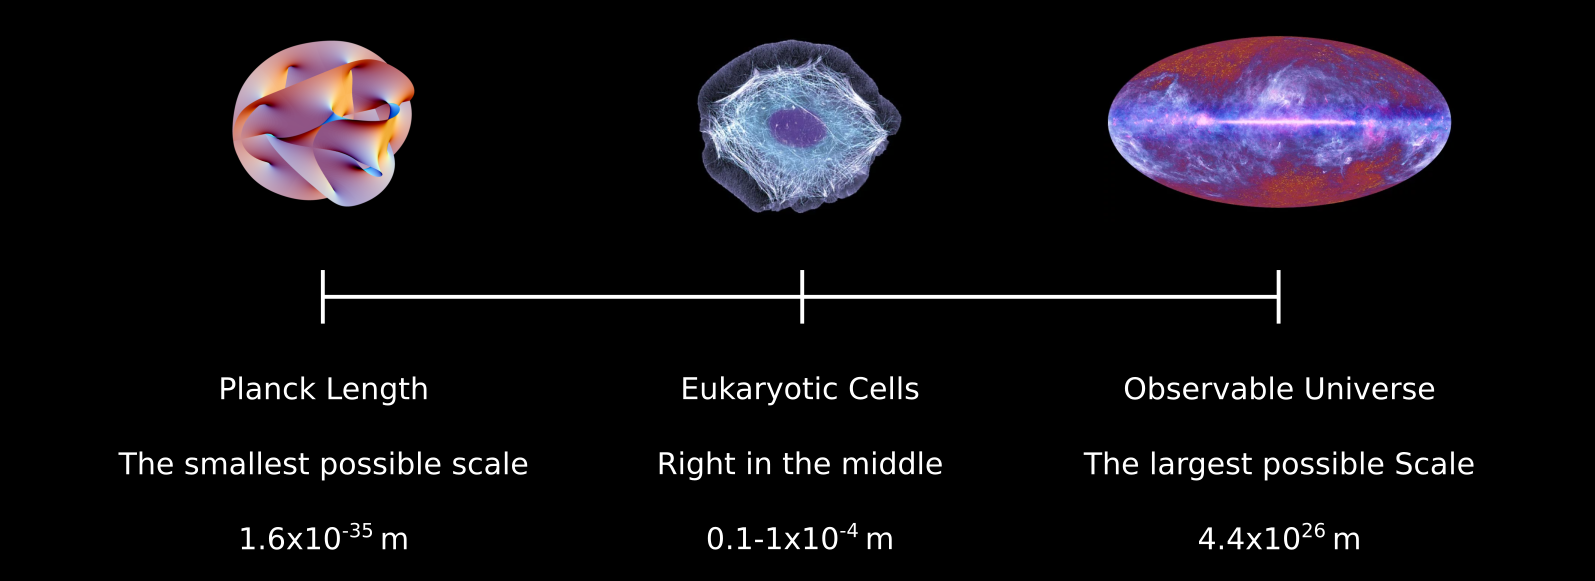
\includegraphics[width=1.0\textwidth]{figures/scales.png}
	\end{center}
	\captionsetup{singlelinecheck = false, justification=raggedright}
	\caption[The Position That Biology Occupies Compared to the Rest of Physics] {\textbf{The Position That Biology Occupies Compared to the Rest of Physics}}{It just so happens that if you plot the size of everything  in the universe on a log scale, eukaryotic cells fall right in the middle. A physicist can talk about both ends of this scale, we should learn something about the middle too.}
	\label{length_scales}
\end{figure}

Biological systems are not homogeneous. If you look at your hand, you will notice hair, pores, dry skin, dead skin, perhaps even tendons and muscles twitching beneath a faint web of ghostly blood vessels. If you were to pluck a single cell from anywhere in this hierarchy and place it under a powerful microscope, you would just be able to make out some of the organelles inside that cell. The size, shape and function of the organelles would be different if the cell was taken from somewhere else in your body. Within and between each those organelles is a wet, salty dance of molecular machines called proteins, which we will study in detail. The length scales of this journey from your arm to a single protein spans 8 orders of magnitude in length.\footnote{ from the size of your hand to the size a single protein spans from $10^{-1}$m  to $10^{-9}$m respectively.} At each step along the way, there is an army of experts studying different phenomenon at that length scale. 

Note for example how the publications arising from this thesis have many authors. Each researcher specialises, not unlike their cells, in a specific discipline. It is only by working together that can we hope to understand the whole organism.

%\footnote{I just noticed that the words organ, organism and organisation all contain the Greek root ``organon" meaning ``tool". Someone should look into that. }

%\interfootnotelinepenalty=10000
If the reader is anything like myself they will find the amount of required knowledge to study biology a substantial barrier to entry. It is quite difficult at first to figure out what questions to ask or even which subfields to study to alleviate this confusion. These challenges can be tackled by cultivating a broad coalition of connections---speak to medical doctors, clinicians, evolutionary biologists \cite{dawkins1989, dawkins2016}, philosophers, molecular biologists, biochemists, cell biologists\cite{pollard2016}, geneticists, bioinformaticians, theoretical chemists, computer scientists, neuroscientists, physicists, mathematicians, everybody. It will take time but remain patient and you will find that a physics motivated approach can indeed explain and eventually predict outcomes in biological experiments. A broad world view awaits you and it's really quite fun. 
%If the reader is anything like myself they will find the amount of required knowledge to study biology a substantial barrier to entry. It is quite difficult at first to figure out what questions to ask or even figure out which subfields to study to alleviate this confusion. These challenges can be tackled by cultivating a broad coalition of connections; speak to medical doctors, clinicians, evolutionary biologists \cite{dawkins1989, dawkins2016}, philosophers, molecular biologists, biochemists\footnote{These last two are in fact different subfields but like many in this list it'll take you some time to understand the subtle differences which define each one.\enlargethispage{-\baselineskip}}, cell biologists, geneticists, bioinformaticians, theoretical chemists, computer scientists, neuroscientists, physicists, mathematicians, everyone. It will take time but remain patient and you will find that a physics motivated approach can indeed explain and eventually predict outcomes in biological experiments. A broad world view awaits you and it's really quite fun. 

If this is indeed read by a future trainee, I hope the physics focussed philosophy in the introduction of chapter \ref{chap:introduction} and the literature review of simulation techniques in chapter \ref{chap:methods} can serve as a road map---but a physicist studying biology will be best served by nurturing a strong base in electrodynamics and statistical mechanics \cite{griffiths2017, reif2009, zuckerman2010}. One particularly thorny issue for such a reader is that the field is now progressing so quickly that I'm sure much of this thesis will be out of date by the time it's read by anybody I'd hope to train. But that's just one of the things that makes biophysics so exciting. Shoot me an email if you want help \href{mailto:miro.astore@gmailcom}{miro.astore@gmail.com}. Hopefully I'm still in the biophysics game.

The task ahead is immense. We're still not exactly sure how many unique proteins are expressed by the human genome, but it's upward of 20 thousand \cite{salzberg2018}. By contrast, this thesis represents an all consuming effort by a single PhD student running decades worth of simulations to make incremental progress in the study of a single one. There is so much to do. Good luck, I suggest you pack a towel \cite{adams1979}. 

%}
%=======================================================================================%
% the main points of this introduction are 
% outline the complexity of biological systems for physicists
% 	> even though our theoretical models should preidct everything on the energy and length scales of biology we can't because of their heterogeneity.
%   > Give examples of the heterogenaity 
% Give some points on the history of molecular biophysics  
%   >  Hodgkin-Huxley Models
%   > Gramicidin 
% Point out how Cystic Fibrosis is an expression of this progression, going from genotype to phenotype using an ion channel to teach us biophysics. 
% conclusion.
\chapter*{Foreword}
\markboth{Foreword}{Foreword} 
%\lhead{\emph{Foreword}}
\label{chap:foreword}
\chapquote{I've never held a pipette} {}

The more I wrote of this thesis the more I found myself writing down things I wish I'd known when I first started studying biophysics. I was writing for my past self. Hence, I think the audience for this thesis would be those with a loose grasp of undergraduate physics. The most difficult thing for this audience will not be the mathematics or technical content herein, but rather the breadth of biochemical pre requisites to understand the scope of the contents. I have not had time to write an introduction to molecular biology, so I recommend a physics based introduction to those concepts such as those found in ``The Physical Biology of the Cell" \cite{phillips2012}. For more intensive biology focussed introduction there is ``Cell Biology"\cite{pollard2016}. On this note of pedagogy, some care has been taken to name certain authors to give the reader a kind of anchor to keep track of the literature. Similarly, when a technical concept is mentioned, I have searched for a useful review article, book or explainer. So please take such citations as reading recommendations \cite{dawkins1989, hofstadter1999}.

\begin{figure}[h]
	\begin{center}
		\includegraphics[width=0.9\textwidth]{figures/myelin.jpg}
	\end{center}
	\captionsetup{singlelinecheck = false, justification=raggedright}
	\caption[Nerve Cross Section by David Goodsell] {\textbf{Nerve Cross Section by David Goodsell}}{David Goodsell is an artist who produces water paintings of cellular environments. Many of his works can be downloaded and used \href{https://pdb101.rcsb.org/sci-art/goodsell-gallery}{for free}. He has also written many books and articles which would serve as a light, layperson friendly introduction to molecular biology \cite{goodsell2009, goodsell2018, goodsell2020}. This particular painting depicts a nerve fibre (blue) wrapped in an insulating myelin sheath (yellow). Electrical signals propagate into the page, via voltage gated sodium and potassium protein ion channels at the edge of the nerve\cite{goodsell_nerve}. We will discuss the discovery and details of this mechanism in the next chapter. They were critical to the development of biophysics.}
	\label{goodsell_figure}
\end{figure}

When I first started performing these simulations, I didn't even know what a protein was, and I have still not taken a single course in biology or chemistry. But for the past 4 years I have been captivated by the seemingly infinite complexity in biological systems. For some examples, please take an opportunity to treat yourself to the fabulous work of \href {https://pdb101.rcsb.org/sci-art/goodsell-gallery}{David Goodsell} in figure \ref{goodsell_figure}. 

I've found that the mindset for solving biological problems feels very different to the narrowed focus we cultivate in students studying idealised problems in mathematics and physics. The problems are more specific and the solutions are less general. For example, plasma physicists may use the same mathematical tools to describe materials as diverse as the dense stellar core to the sparse intergalactic nebulae. These objects span 28 orders of magnitude in density \cite{chen2018}.\footnote{From $10^{34}-10^6$ charged particles per meter cubed respectively.} Would that we were so lucky in biology, where we struggle to apply same physical models to deal with phenomenon across a single order of magnitude. All the same, it appears increasingly clear to me that biological phenomenon occupy a special place in the universe (Figure \ref{length_scales}). 


\begin{figure}
	\begin{center}
		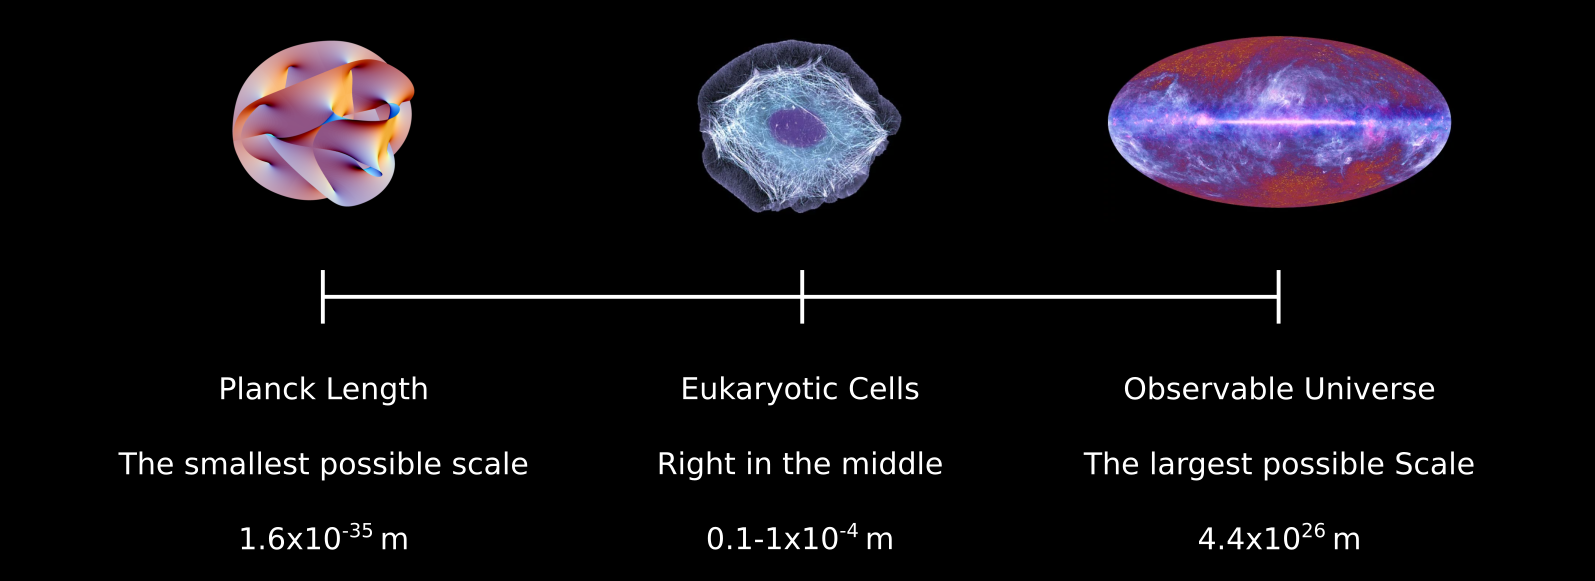
\includegraphics[width=1.0\textwidth]{figures/scales.png}
	\end{center}
	\captionsetup{singlelinecheck = false, justification=raggedright}
	\caption[The Position That Biology Occupies Compared to the Rest of Physics] {\textbf{The Position That Biology Occupies Compared to the Rest of Physics}}{It just so happens that if you plot the size of everything  in the universe on a log scale, eukaryotic cells fall right in the middle. A physicist can talk about both ends of this scale, we should learn something about the middle too.}
	\label{length_scales}
\end{figure}

Biological systems are not homogeneous. If you look at your hand, you will notice hair, pores, dry skin, dead skin, perhaps even tendons and muscles twitching beneath a faint web of ghostly blood vessels. If you were to pluck a single cell from anywhere in this hierarchy and place it under a powerful microscope, you would just be able to make out some of the organelles inside that cell. The size, shape and function of the organelles would be different if the cell was taken from somewhere else in your body. Within and between each those organelles is a wet, salty dance of molecular machines called proteins, which we will study in detail. The length scales of this journey from your arm to a single protein spans 8 orders of magnitude in length.\footnote{ from the size of your hand to the size a single protein spans from $10^{-1}$m  to $10^{-9}$m respectively.} At each step along the way, there is an army of experts studying different phenomenon at that length scale. 

Note for example how the publications arising from this thesis have many authors. Each researcher specialises, not unlike their cells, in a specific discipline. It is only by working together that can we hope to understand the whole organism.

%\footnote{I just noticed that the words organ, organism and organisation all contain the Greek root ``organon" meaning ``tool". Someone should look into that. }

%\interfootnotelinepenalty=10000
If the reader is anything like myself they will find the amount of required knowledge to study biology a substantial barrier to entry. It is quite difficult at first to figure out what questions to ask or even which subfields to study to alleviate this confusion. These challenges can be tackled by cultivating a broad coalition of connections---speak to medical doctors, clinicians, evolutionary biologists \cite{dawkins1989, dawkins2016}, philosophers, molecular biologists, biochemists, cell biologists\cite{pollard2016}, geneticists, bioinformaticians, theoretical chemists, computer scientists, neuroscientists, physicists, mathematicians, everybody. It will take time but remain patient and you will find that a physics motivated approach can indeed explain and eventually predict outcomes in biological experiments. A broad world view awaits you and it's really quite fun. 
%If the reader is anything like myself they will find the amount of required knowledge to study biology a substantial barrier to entry. It is quite difficult at first to figure out what questions to ask or even figure out which subfields to study to alleviate this confusion. These challenges can be tackled by cultivating a broad coalition of connections; speak to medical doctors, clinicians, evolutionary biologists \cite{dawkins1989, dawkins2016}, philosophers, molecular biologists, biochemists\footnote{These last two are in fact different subfields but like many in this list it'll take you some time to understand the subtle differences which define each one.\enlargethispage{-\baselineskip}}, cell biologists, geneticists, bioinformaticians, theoretical chemists, computer scientists, neuroscientists, physicists, mathematicians, everyone. It will take time but remain patient and you will find that a physics motivated approach can indeed explain and eventually predict outcomes in biological experiments. A broad world view awaits you and it's really quite fun. 

If this is indeed read by a future trainee, I hope the physics focussed philosophy in the introduction of chapter \ref{chap:introduction} and the literature review of simulation techniques in chapter \ref{chap:methods} can serve as a road map---but a physicist studying biology will be best served by nurturing a strong base in electrodynamics and statistical mechanics \cite{griffiths2017, reif2009, zuckerman2010}. One particularly thorny issue for such a reader is that the field is now progressing so quickly that I'm sure much of this thesis will be out of date by the time it's read by anybody I'd hope to train. But that's just one of the things that makes biophysics so exciting. Shoot me an email if you want help \href{mailto:miro.astore@gmailcom}{miro.astore@gmail.com}. Hopefully I'm still in the biophysics game.

The task ahead is immense. We're still not exactly sure how many unique proteins are expressed by the human genome, but it's upward of 20 thousand \cite{salzberg2018}. By contrast, this thesis represents an all consuming effort by a single PhD student running decades worth of simulations to make incremental progress in the study of a single one. There is so much to do. Good luck, I suggest you pack a towel \cite{adams1979}. 

% the main points of this introduction are 
% outline the complexity of biological systems for physicists
% 	> even though our theoretical models should preidct everything on the energy and length scales of biology we can't because of their heterogeneity.
%   > Give examples of the heterogenaity 
% Give some points on the history of molecular biophysics  
%   >  Hodgkin-Huxley Models
%   > Gramicidin 
% Point out how Cystic Fibrosis is an expression of this progression, going from genotype to phenotype using an ion channel to teach us biophysics. 
% conclusion.
\chapter{A Physical Introduction to Theoretical Biology}
\pagenumbering{arabic}
\setcounter{page}{1}
\label{chap:introduction}
%\chapquote{Whatever complexity means, most people agree that biological systems have it.} {Frauenfelder and Wolynes \cite{frauenfelder1994}}

\begin{chapquote}  {Frauenfelder and Wolynes \cite{frauenfelder1994}}
Whatever ``complexity" means, most people agree that biological systems have it.
\end{chapquote}

%\vspace
\section{Thesis and Chapter Summary}

This thesis seeks to apply a philosophy of molecular biophysics, to demonstrate its capability to investigate pressing problems in biology and medicine. In particular, we will use molecular dynamics (MD) to look at how a specific gene misfunctions to cause disease. The disease in question is Cystic Fibrosis (CF), and it is caused by the misfunction of a protein called the Cystic Fibrosis Transmembrane Conductance Regulator (CFTR). These MD techniques will allow us to formulate a model of CFTR's misfunction which we hope will direct research efforts and allow more patients suffering from CF to access life saving medication. 

In this first short chapter we will quickly build a philosophy which outlines how to look at biology through the lens of a physicist. To do this we will first outline what the goal of a physicist is: to create abstract formalisms which can be used to model the natural world. We will then observe what makes the construction of such formalisms so difficult for biological problems. 

These difficulties have often led biophysicists to study ion channels. Because of their simplicity, and their importance to cellular function, these molecules have served as laboratories to understand more complex biological systems, such as whole cells or organisms. 

Chapter \ref{chap:methods} will describe the chemical and numerical simulation techniques we have used to study the CFTR protein system in detail, while chapter \ref{chap:cftr} gives an overview of the CFTR system itself, and also a set of \textit {in vitro} assays which compliment our computational modelling.  Chapters \ref{chap:I37R}, \ref{chap:R352Q}, \ref{chap:S945L} and \ref{chap:opening} demonstrate the details of how a diverse application of the simulation techniques in chapter \ref{chap:methods} can be used to discover the unique modes of misfunction in CFTR. In combination with \textit {in vitro} cellular techniques, these simulation results prove that these existing drug regimens can rescue many molecular defects. Finally, chapter \ref{chap:perspective} ties together these results to argue for a physical model which elucidates the mechanism of action for cystic fibrosis drugs. Armed with this model we will work through the available literature and identify some priorities for future studies using molecular modelling for cystic fibrosis research. 

%In chapters \ref{chap:methods}, \ref{chap:cftr} and \ref{chap:perspective} considerable care has been taken to give an overview of the many aspects of computational methods using MD and the cellular, molecular and clinical research into CF to give future readers a detailed reference text should they too wish to study CF.

We hope this small example can demonstrate the utility of physics expertise for the field of molecular medicine. We anticipate that such methods will only grow in power with improvements in computational and experimental techniques.

\section{What is Physics?}
\label{WIP}
Before I started university I described physics as ``the study of how things move". Although intuitive, this description does not shed light on the philosophy of doing physics which make it such a powerful tool for understanding the natural world. When we create a predictive physical theory, we first carefully define a formalism motivated by patterns we see in the world around us. Then, using mathematics, the implications of this formalism are built up to make predictions about measurable phenomena. Should the predictions from the formalism agree with experimental results, it validates the formalism, giving rise to a physical theory. This is what makes physics feel like the most ``fundamental" of the natural sciences.

%\footnote{The natural sciences include chemistry, biology, physics.  Mathematics and logic are forms of the formal sciences, which we rely on heavily as natural scientists. }

These formalisms make use of many mathematical objects. Examples you might be familiar with include:
\begin{itemize}
\item The gas of hard spheres, which we use to derive the Boltzmann's kinetic theory of gasses.  
\begin{equation}
	\label{hard_spheres}
	\frac{\partial f_1}{\partial t} + \frac{\bold{F}}{m}\cdot\nabla_\bold{r} + \bold{v} \cdot \nabla_\bold{r} f_1 =  \int \int (f'_1f'_2 - f_1 f_2) \tilde \kappa d \hat \kappa d \bold{v}_2.
\end{equation}

\item The interacting electric and magnetic vector fields in Maxwell's laws of electromagnetism \cite{griffiths2017}.
\begin{equation}
	\begin{aligned}
	%\nabla \dot \mathbf{E} = \frac{\rho}{\epsilon_0}
		\nabla \cdot  \mathbf{E} &= \frac{\rho}{\epsilon_0} \qquad & \nabla \cdot  \mathbf{B} &= 0 \\
		\nabla \times  \mathbf{E} &= -\frac{\partial \mathbf{B}}{\partial t} \qquad &  \nabla \cdot  \mathbf{B} &= \mu_0 \big(\mathbf{J} + \epsilon_0 \frac{\partial \mathbf{E} } {\partial t }\big).
	\end{aligned}
\end{equation}

%\partial_\alpha F^{\alpha \beta} = \frac{4\pi}{c} J^\beta
\item The Riemannian manifolds which define the curvature of spacetime in Einstein's theories of relativity \cite{carroll2019}.
\begin{equation}
	G_{\mu \nu} + \Lambda g_{\mu \nu} = \kappa T_{\mu \nu}.
\end{equation}

\item The complex probability waves which evolve according to Schr\"oedinger's equation, describing quantum mechanics \cite{griffiths1994}. 

\begin{equation}
	i \hbar \frac{d}{dt} | \psi (t) \rangle = \hat {H} | \psi (t) \rangle .
\end{equation}
\end{itemize}

As biophysicists we would wish to find the most basic formalisms for biological phenomenon, so we can fully understand the function of an organism. The quest for such a formalism has an interesting origin. In 1944 Erwin Schr\"oedinger wrote an essay titled ``What is Life?" This remarkable work was written before the discovery of DNA's structure or the maturation of information theory. Schr\"oedinger used first principles in thermodynamics and quantum mechanics to speculate at the nature of life at the atomic level. The most remarkable thing about this essay is how much the author got right. 

He observed that since organisms exist at temperatures on the order of 300 Kelvin, the physical encoding of genetic information inside cells must be chemical in nature---since at such temperatures the physical arrangements of atoms would be unstable without chemical bonds. By estimating the amount of information that could be stored in an arrangement of atoms, Schr\"oedinger posits the existence of what he calls an ''aperiodic crystal". Although not a crystal in the rigorous sense, the double helix structure of DNA is not far from such an analogy. As Figure \ref{dna_structure} shows, the DNA double helix is a combination of periodic and aperiodic elements, not too different from how one might visualise a one-dimensional aperiodic crystal \cite{varn2016}. This allegory is an example of how physical principals can be used to direct questions in fundamental biology. In fact, James Watson credited Schro\"edinger's book as one of his influences in how he visualised the structure of the DNA before its discovery through X-ray crystallography \cite{watson2010}.

\begin{figure}
	\begin{center}
		\includegraphics[width=1.0\textwidth]{figures/dna_backbone_aperiodic_crystal.pdf}
	\end{center}
	\captionsetup{singlelinecheck = false, justification=raggedright}
	\caption[The Structure of DNA has Periodic and Aperiodic Elements] {\textbf{The Structure of DNA has Periodic and Aperiodic Elements}}{Although not a crystal, the structure of DNA has some periodic and some aperiodic elements. This is reminiscient of Schr\"oedinger's speculation that genetic information is chemically encoded in an aperiodic crystal. }
	\label{dna_structure}
\end{figure}

In this example, Schr\"oedinger naturally chose a formalism of interacting atoms, mostly consistent with the statistical mechanics in equation \ref{hard_spheres}, to arrive at his model of an aperiodic crystal. In this thesis we will use a more careful, but similar formalism to study the function of the CFTR protein. We will outline this formalism in detail in chapter \ref{chap:methods}. The goal of chapters \ref{chap:cftr}-\ref{chap:opening} is then to collect evidence in order to develop a physics inspired model of for the treatment of Cystic Fibrosis disease, which we will propose in chapter \ref{chap:perspective}. The model we arrive at is more abstract than physicists are used to, and the next section will explore why this is often the case for biological systems.
 
%Somewhere on the scale between a single protein and a single cell this is what we consider "life". We have single unicellular organisms but we don't have uniproteomic organisms. So the fundamental length scale of life is somewhere between $10^{-10}m$ and $10^{-3}m$. This is the first loop in our strange loop.

%Biological strange loops would not seem to be as self similar as the clean nice logics in the strange loop of the Godelian knot. Why is this?

\section{The Physics Inside your Cells}
%purpose of this section is to 

Why can't I write down an equation which will tell me how long I will live? Or how tall I will grow?

These might seem like odd questions but if you asked a physicist how much power it would take to ionise a gas or how long it will take a black hole to evaporate itself out of existence, they would have a tool kit of highly accurate models to help them calculate solutions. 

To understand why the first set of problems are so much more difficult for physicists, we will analyse the cases where physics fails. Any physical theory may fail for one of the following three reasons: 

\begin{itemize} 
	\item The physicist does not have sufficient computational power to integrate the formalisms in the relevant theory, so they cannot make predictions about a specific phenomenon.

		\item The physicist lacks sufficient data, so they cannot specify reasonable initial conditions for the calculations with the formalism. 

		\item The phenomenon in question lies outside the applicable energy or length of the physical theory.This would occur, for example, if we used Newton's theories of gravity to predict the motion of an object around a super-massive black hole---here we would instead need Einstein's general theories of relativity \cite{picker2022}.

\end{itemize}

From the perspective of fundamental physics, quantitative theories of biology fail for one of the first two reasons. Given the energy and length scale of biological systems, we currently possess the necessary theoretical tools to simulate every interaction inside a living being \cite{carroll2021}. 

The difficulty of studying biology then, does not arise from a lack of physical understanding. As we will see in chapter \ref{chap:methods} the physics of the molecular interactions in living things is surprisingly simple. Rather, the difficulty of biological problems arises from the sheer number of interactions we must consider. Inside cells we find proteins, lipids, solvents, salts each with their own physical properties. Therefore, biophysics distinguishes itself from more traditional physics by considering systems that are both highly heterogeneous and anisotropic. This aspect of biological systems makes it difficult to scale up our formalisms to make predictions using human tractable mathematical tools---meanwhile, computational engines can only help so much. Hence, we have to be careful about which systems we study with our available toolkit. When their computational or theoretical tools were lacking, physicists often turned to ion channels as laboratories to develop and test biophysical theories \cite{moy2000, corry2000}.

%For biological systems there appears to be too much complexity for such analogies to have the same level of success. 

%Although considerable success can be found in modelling biology with formalisms that do not stem directly from fundamental physics, such models must be tailor made in order to treat specific phenomenon \cite{phillips2012}. The advantage of MD and the formalism of interacting atoms in chapter \ref{chap:methods} is that they are the most accurate available to the biophysicist. The issue is the considerable computational load attached to them. 

%Thus, in order to move towards more predictive theories of biology it is necessary to develop layers of physical theories applicable in different contexts. One form of this from fundamentals approach is the simulation of every atom in a biological system. Although computationally expensive, this approach has been proven necessary when studying the molecular details of proteins, due to the heterogeneous nature of biological systems . 


%One of the things we're trying to do with molecular dynamics is fill in the gap left by the sequence->function paradigm which is internalised in current understandings of molecular biology. We usually talk about how the sequence of the gene defines its function because it gives the protein its structure but really there is a considerably larger amount of regulatory pressure exerted by the environment. This is what is missing from the sequence alone paradigm.

%Biological systems exhibit such a problem for the physicist because unlike the above problems it is extremely hard to pick out a fundamental unit to even begin our upwards journey. An evolutionary biologist might say to choose the "gene" but this is actually far too high in our spatial heirarchy already. Really, a gene is only meaningful to the dance of life if it has partners to dance with. 

%A coil of DNA in water doesn't really do much in solution except decay without machinery that can preserve, read, translate and replicate it. The gene is an emergent property, we have to go deeper. 

%So, what are the gene's partners? 

%A slew of biological machinery that mostly take the form of proteins. These proteins are a special case of chemistry, with many observable functions. Their sequence is  coded by the DNA in something reminiscent of a strange loop \cite{hofstadter2007}. 

%This self referential loop is one of the reasons biology is so difficult. Since we know that this strange loop is kicked off by atomic interactions we will start there. As we are taking a physical, pragmatic approach here it would make sense to begin with the protein, after all, they stave off the march of entropy constantly trying to eat up all of your cells. It also just so happens that they are much easier to understand computationally since their motions are faster and more flexible. 

%The first level sub cellular organisation is perhaps the most intimdating first step for me personally after spending 4 years simulating a single protein. Glimpsing the complexity within a single one of these molecules has been one of the most existential experiences of my life but the knowledge that there are astronomical numbers of these things inside me all of the time terrifies me.

%It is hoped that illustrating the monumental amount of both intellectual effort and material resources of incrementally increasing the understanding of a single protein amongst the 23000 or so encoded in our genome will give the reader and understanding of how we might continue our quest to understand the molecular dance that plays within all of us.

%After this things start to run away from me with my handful of GPUs and limited patience. So in this thesis we will only discuss single proteins.

\section{Using Ion Channels as Natural Laboratories to Study Biophysics}
\label{ion_channel_laboratories}

Ion channels are a special kind of protein which allow the passage of charged particles to pass across the membrane of a cell. They are excellent laboratories for the study of biophysics for two reasons. Firstly, it is very easy to measure their activity with a technique called electrophysiology which we will briefly explore in chapter \ref{chap:cftr} \cite{hille2001}. Secondly, they are critical to the health and function of cells. As cell biology has advanced, it has become increasingly clear that the level of polarisation (potential difference from the inside to the outside) in a cell is critical to its function. Cell polarisation regulates many chemical reactions \cite{catterall2011, muthuswamy2012, levin2014, levin2014a}.\footnote{A back of the envelope calculation reveals that a -100mV resting potential is a 2.5 kcal/mol barrier to the transport of molecular species with a charge of -1e into the cell. This is not an insignificant energy contribution.} 

It is perhaps then not surprising but nonetheless remarkable that ion channels are the targets of 19\% of clinically approved drugs \cite{santos2017}. However, there is much more work to be done, as candidate drugs are often insufficiently selective for the desired ion channel, leading to sometimes lethal side effects \cite{stansfeld2006, kaczorowski2008, waszkielewicz2013}.

Historically, ion channels have served as a testing ground for biophysical models. The first interest in modelling their behaviour comes from the experiments of two biophysicists, Andrew Hodgkin and Alan Huxley. They threaded silver wires through the thick nerves of a giant squid and measured the current running through the nerve in response to electrical stimulation. What they found was intriguing. Signals would only propagate down the nerve when the input signal was of a sufficient high voltage. They managed to match their experimental data with a model comprised of the following set of ordinary differential equations:

\begin{equation}
	\label{hh_equations}
\begin{aligned}
	I = C_m \frac{dV}{dt} + \bar{g}_K& n^4 (V - V_K) + \bar{g}_{Na} m^3 h (V - V_{Na} ) + \bar{g}_l (V-V_l) , \\ \\
	\frac{dn}{dt} &= \alpha_n(V)  (1-n) - \beta_n(V)  n, \\ \\
	\frac{dm}{dt} &= \alpha_m(V)  (1-m) - \beta_m(V)  m, \\ \\
	\frac{dh}{dt} &= \alpha_h(V)  (1-h) - \beta_h(V)  h.  
\end{aligned}
\end{equation}

Here, the $n,\ m$ and $h \in [0,1]$ parameters are associated with potassium channel subunit activation, sodium channel subunit activation, and sodium channel subunit inactivation, respectively. $C_m$ is the capacitance of the lipid membrane per unit area, and $\bar{g}_i$ is the maximal conductance allowed across the membrane, per unit area. The terms $V_i$ denote either the total voltage, or the contribution to the total from a specific charged species. 

The solutions to the Hodgkin-Huxley model allow us to mathematically discover and describe several important cellular functions. The model encodes both the existence of a cell's resting potential and the behaviour of selective voltage-gated ion channels. Even today, the molecular mechanisms behind these discoveries are used to understand protein and cellular function \cite{aidley1996}. This curve created by the action potential is a common sight in many physiology textbooks, and it is in fact a solution to this coupled set off ODES \cite{pollard2016}.

\begin{figure}
	\begin{center}
		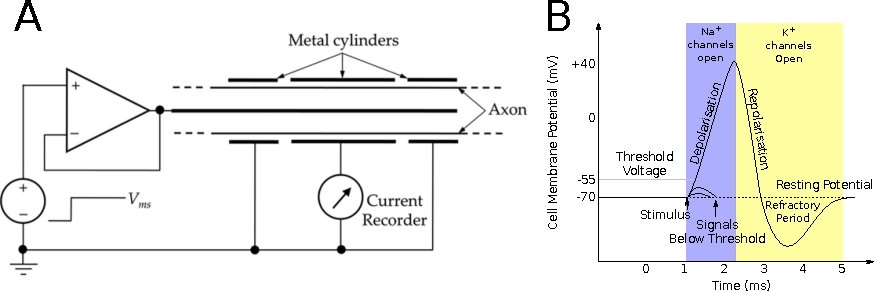
\includegraphics[width=0.9\textwidth]{figures/Hodgkin-Huxley_action_potential.pdf}
	\end{center}
	\captionsetup{singlelinecheck = false, justification=raggedright}
	\caption[The Action Potential is a Solution to the Hodkin-Huxley Model] {\textbf{The Action Potential is a Solution to the Hodgkin-Huxley Model }}{ A) The ``voltage clamp" experimental set up which was used to study nerve impulses \cite{hodgkin_huxley_figure_website}. A giant squid nerve was submerged in sea water and an electrode was threaded through it as shown. The voltage was recorded as impulses were fired into the nerve. B) The shape of the action potential is a familiar sight in many physiology textbooks. The physical basis for its shape was realised through the mathematical modelling of Hodgkin and Huxley which won them the 1963 Noble Prize in physiology or medicine. This discovery is an example of the physiological importance of ion channels and also how deep theoretical insight can lead to predictive models of living systems \cite{hodgkin1952, hodgkin1952a, hodgkin1952b, hodgkin1952c, hodgkin1952d}.}
	\label{action_potential_graphic}
\end{figure}

The equations in the model \href{hh_equations}{above} are an example of the development of a mathematical formalism which is not fundamental in the same way as the equations at the beginning of section \ref{WIP}. But rather, the model above is built for an express purpose: to predict and describe the propagation of signals through a nerve. This model shows how quantitative thinking can lead to insights in biology. The sheer complexity of biology demands this of us. We cannot create complete theories so we must find useful formalisms for small domains of the problem space.

\begin{figure}
	\begin{center}
		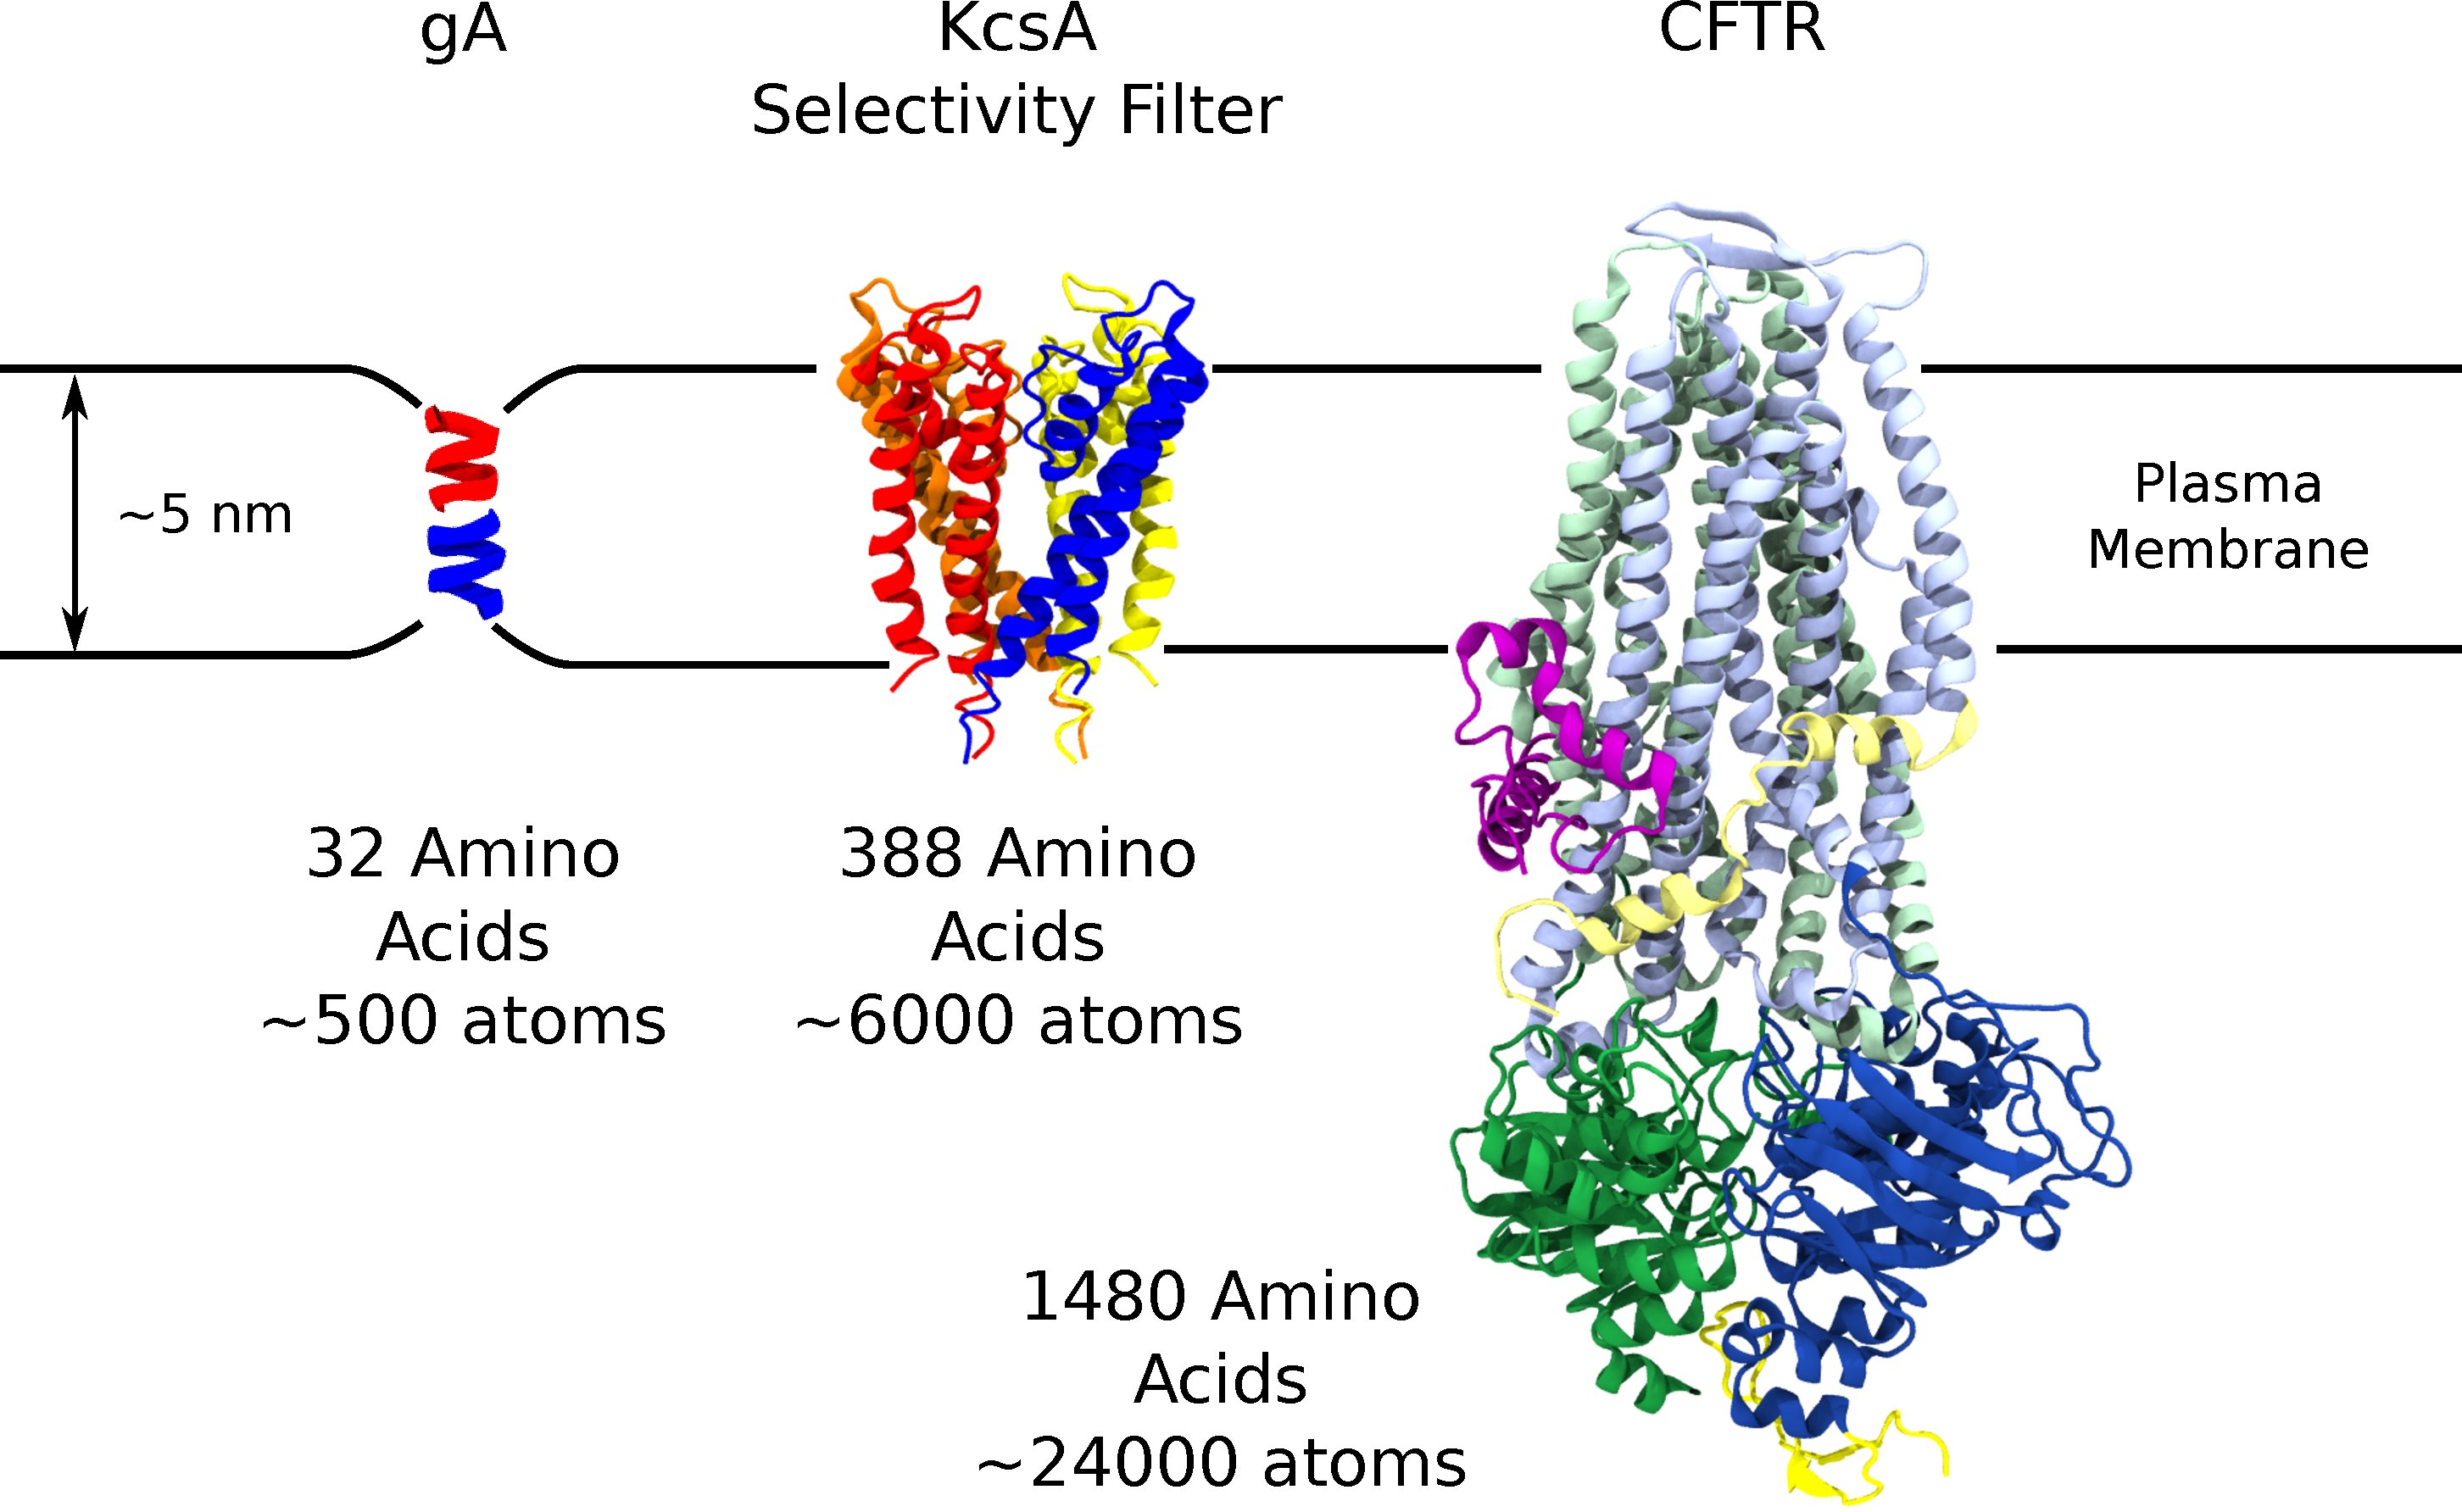
\includegraphics[width=0.8\textwidth]{figures/ion_channel_progression.pdf}
	\end{center}
	\captionsetup{singlelinecheck = false, justification=raggedright}
	\caption[Different Ion Channels Amenable to Molecular Simulation] {\textbf{Different Ion Channels Amenable to Molecular Simulation}}{Gramicidin A was initially used as a toy model to test different \textit{in silico} modelling techniques (PDB ID 1NT5) \cite{sham2003}. KcsA, is a bacterial potassium channel. This structure only comprises the pore domain, also called the selectivity filter (PDB ID 1BL8) \cite{doyle1998}. This structure drew interest because potassium channels play an important role in the function of cells. Finally, the CFTR anion channel about which this thesis is written (PDB ID 6MSM) \cite{zhang2018a}. In the course of 30 years we have gone from simulating just a few nanoseconds of Gramicidin A to collecting almost half a millisecond of data for this thesis by simulating the much larger CFTR. This heralds an exciting future for computational biophysics \cite{roux1993}. What is even more exciting will be the next 30 years. At the time of writing, a computational engine named Anton 3 has come online. This purpose built computer could perform all the calculations in this thesis in less than a week \cite{jones2022, russell2021}. That's not a week in parallel, that's in serial!}
	\label{ion_channel_progress}
\end{figure}

In this thesis we aim to do something similar. By building up from the fundamental physics outlined in chapter \ref{chap:methods}, we will build a model for the dysfunction of a single gene (CFTR), to understand a disease (CF). Again, we do not possess sufficient computational power to produce a complete physical model of CF, so we will have to settle for a qualitative model, which we will outline in chapter \ref{chap:perspective}. 

%The measurements and modelling they carried out gave an exciting set of results. They found that the cell had to maintain a constant voltage gradient, they discovered that the presence of voltage gated ion channels and cation selective ion channels \cite{hodgkin1952}. Each of these features, motivated by mathematical modelling have been found to be critical to the functioning of the cell and fundamental to the foundation of molecular biophysics.    

\subsubsection{Computer Modelling the Dynamics of Ion Channels}
Motivated by the advances in cell biology that arose from the Hodgkin-Huxley model, early adopters of computational biophysics such as Martin Karplus, Beno\^it Roux, Klaus Schulten, J. Andrew McCammon, Shin-Ho Chung, Mark Sansom, Helmut Grubm\"uller, Serdar Kuyucak and Toby Allen devoted significant parts of their career to studying ion channels \cite{mccammon1977, sansom1991, roux1991, roux1993, sansom1991, tajkhorshid2002, degroot2001, allen2003, allen2004, chung2002, tieleman2001}. 

These early studies usually focussed on gramicidin A (gA) because of its small size, its amenability to structural characterisation and the opportunity to compare experimental measurements with \textit{in silico} calculations \cite{urry1971,arseniev1985,wallace1986,wallace1998}. This small antibacterial peptide assembles into a coil which selectively allows the passage of potassium ions in the cell walls of gram-positive bacteria. This bleeds dry the bacteria's internal potassium concentration, which is critical to cellular function \cite{liou2015}. For a long time, gA was the only protein ion channel with its structure determined to atomic resolution. Because ion channels are membrane proteins, it took further advancements in experimental structural biology techniques by Roderick Mackinnon and others to determine the atomistic structures of other channels \cite{kuhlbrandt2014, clapham2003, doyle1998}. 


The careful work on gA enabled the development of theoretical and computational methods which can now be transferred to the more biologically important channels, such as potassium and sodium ion channels \cite{rashid2013, li2021, vandenberg2021,flood2019}. With the ``resolution revolution" in structural biology, driven by the maturation of cryo-EM structural biology and even more recently AI based structure predictions, we are entering an era of structural abundance---there are now literally thousands of biologically relevant targets which we can study with simulations \cite{jumper2021, frank2021, cheng2017a}. 

%This careful work on gA aided the development of many computational techniques. Along with an abundance of protein structures and other experimental advances, of this kind of modelling and experimental techniques the molecular details of the function of ion channels has become accessible to computational techniques \cite{flood2019}. The careful work on gA enabled the development of theoretical and computational methods which could then be transferred to the more biologically important channels such as potassium channels once they were structurally characterised by the laboratories of Roderick MacKinnon and others \cite{rashid2013, li2021, vandenberg2021}. Now with the ``resolution revolution" occurring in structural biology with the maturation of cryo-EM structural biology and now AI based protein predictions we are entering an era of structural abundance. 

In this new era, ion channels will likely continue to be important clinical and biophysical targets. In addition to the propagation of nerve signals we saw in section \ref{ion_channel_laboratories}, they play a critical role in all 5 senses, allowing cells to react to pressure (and hence touch) \cite{chesler2018}, temperature \cite{castillo2018}, pain \cite{kingwell2019}, acids \cite{kweon2013} and smell (in insects) \cite{sato2008}. There is also an exciting subfield emerging which investigates the role of ion channels in the bioelectrical networks which regulate cell morphogenesis and growth \cite{lang2005, sundelacruz2009, levin2014, levin2014a}.

As we have shown, the historical goal of computational biophysicists has been to use whatever physical models and structural information is available, to understand living things at the molecular level (Figure \ref{ion_channel_progress}) \cite{lev2020, chen2021}. In this thesis, we seek to continue this trend, by applying the fundamental physical models described in chapter \ref{chap:methods} to study a disease, Cystic Fibrosis, at the molecular level.

%The availability of protein structures and the maturation of computational methods has enabled diverse studies of ion channels and other protein systems . Some of this progress has been summarised in figure \ref{ion_channel_progress}. In this thesis we have continued this trend, by applying the theoretical and computational techniques to study an ion channel and toward develop a theoretical model which helps us study a disease, Cystic Fibrosis. 

\section{Studying Cystic Fibrosis; Toward a Molecular Theory of Disease.} 

The sad truth of Cystic Fibrosis (CF) is that those afflicted are extremely unlucky. A small change to their genome causes their lungs to fill with sticky mucus and become infected with bacteria---each breath becomes cumbersome \cite{katkin2022}. Historically, diseases have been diagnosed based on symptoms and not causes \cite{foucault1994}. As section \ref{WIP} outlines, this is antithetical to how we would like to study a physical process, even a biological one. 

To build a predictive model, we would like to understand the root cause of a disease so we can predict how to treat it. Discovering this root cause can be extremely difficult and often requires decades of clinical enquiry \cite{dubois2016, tsui2013}. CF has the helpful characteristic of being a monogenic disease, so our molecular theory of this disease can begin by considering a single protein system and then slowly build outward, to  consider other genes which effect the disease as well.

In this way, my motivations for studying the CFTR protein are not solely focussed on treating disease. This problem is also an interesting opportunity to develop molecular theories of biology. This is what motivated the basic biophysical studies in chapter \ref{chap:opening}. 

When understanding CFTR, a helpful perspective can be gained from the following model of protein evolution. It states that the stability of a protein's structure contributes to the overall fitness of an organism by a formula \cite{depristo2005}:

\begin{equation}
	\label{fitness_equation}
	W(\Delta G) \propto \exp\bigg(\bigg[-\frac{\Delta G - \Delta G_{opt}}{\sigma_{\Delta G}}\bigg]^4\bigg) + c.
\end{equation}

Here, $W$ represents the evolutionary fitness of an organism, $\Delta G$ is the folding energy of the protein with a given gene sequence and $\Delta G_{opt}$ is the folding energy of the protein in the average (fit) population. The parameter $\sigma_{\Delta G}$ controls how broad this distribution will be and depends significantly on the protein physics of the gene. Figure \ref{fitness_landscape_figure} demonstrates the types of random walks a gene might take through sequence space, according to this model. 

There are over 400 recorded mutations which cause CF \cite{cftr2}. This indicates that  the CFTR gene exhibits an exceptionally small $\sigma_{\Delta G}$, so the band in the modified gaussian in figure \ref{fitness_landscape_figure}a is very narrow. This means that CFTR sits at the precipice of a daunting cliff in sequence space.  So, by taking small steps in sequence space and figuring out what factors have caused $W$ to decrease, we can try to understand how we might push the needle of protein stability back into the optimal zone. Once we understand how we can do this for CFTR, we can use such thinking to build our methods outward and apply it to other diseases, such as sickle cell anemia, Alzheimer's disease, and Huntington's disease \cite{depristo2005}.

	\begin{center}
		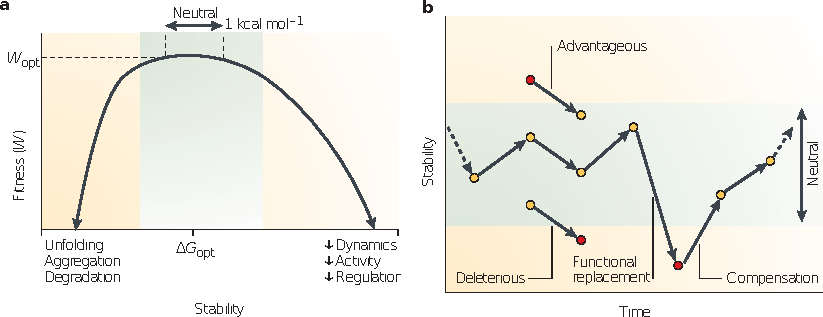
\includegraphics[width=1.0\textwidth]{figures/fitness_landscape_fig.pdf}
	\end{center}
	\begingroup
	\captionsetup{singlelinecheck = false, justification=raggedright}
	\captionof{figure}[A Physical Model to Understand Protein Evolution] {\textbf{A Physical Model to Understand Protein Evolution}}{a) The stability of a protein can be measured by its folding free energy $\Delta G$. This is related to the fitness of an organism $W$ by equation \ref{fitness_equation}. This model gives rise to a peaked distribution which helps us understand how so many mutants can give rise to cystic fibrosis. It appears as though the CFTR gene has an exceptionally narrow $\sigma_{\Delta G}$ and so small changes to the sequence of the gene have a comparatively dramatic effect on the evolutionary fitness of the organism. b) The model in equation \ref{fitness_equation} gives rise to a random walk through sequence space for subsequent generations. In the case of CF, it would appear as though \textit{homo sapiens} are stuck at a specific snapshot in evolutionary time where CFTR may easily lose function. So, without gene therapies which can modify a gene sequence \textit {in vivo}, we must use small molecule drugs and other medical interventions to somehow broaden the peak in equation \ref{fitness_equation}.}
	\label{fitness_landscape_figure}
\endgroup

CF is an excellent disease with which to begin such a project. Due to the array of disease causing mutations which occur across the CFTR protein, there is a large body of literature on its unique function \cite{csanady2019a}. This presents the opportunity to simultaneously perform basic biophysical research, while directly assisting in the improvement of patient outcomes. This is the sort of inquiry which drives basic science forward---combining interesting experimental data into theoretical models to make testable predictions. The aim of this thesis is to build a model to help direct efforts which will hopefully produce better patient outcomes. In chapter \ref{chap:perspective}, we will combine evidence from the existing literature with our biochemical and simulation results to build our predictive model. It is hoped that this model can help direct future strategies to treat CF.

%As we will see in chapter \ref{chap:cftr}, the integration of basic biological research into the treatment of disease can drastically improve patient outcomes. In this particular context, we have studied a single gene. But eventually, similar thinking will be able to build out our understanding consider multiple genes in as much detail, giving us a more complete picture of both life and disease, heralding the exciting future for biophysics. 

\section{The Future is Biological}
Biological sciences have important applications in medicine, agriculture and increasingly, manufacturing \cite{anonymous2019, scown2022}. We are in the midst of developing biology from a descriptive, to a predictive science \cite{kochanski1973,liu2005, mogilner2016, covert2021, jumper2021}. This transition is being driven by the combination of refined experimental techniques, rich datasets, strong theories and powerful computational engines. This is exciting because biological systems have happened upon ingenious solutions to some very difficult problems with the help evolution \cite{dawkins1989, dawkins2016}. Evolution has done much of the hard work for us, and as we understand it better, we can begin to apply its solutions to our own problems \cite{benyus2009, wang2021a, arnold2018}.

Throughout science, the integration of experimental data with theoretical models leads to new discoveries. In the case of biology, wet lab scientists take advantage of experimental techniques which allow them to understand the structure and dynamics of living things from the top down. The finer the experimental instrument, the finer the detail they may resolve. Conversely, computational and theoretical biologists take a bottom up approach. Like physicists, they aim to take the granular details of a system and integrate them upwards, to model and predict the macroscopic behaviour of a system. 

With more powerful computers and more detailed theoretical models, theorists can make predictions about the behaviour of more complex systems. What is so exciting about the current era of biological research is that the domains of these two approaches are beginning to overlap, where they can synergize and drive further breakthroughs \cite{anonymous2019}.

This has been happening in physics for decades, resulting in world changing breakthroughs like telecommunications, nuclear power and transistors \cite{wu2009}. The reason this has been possible for physicists is that the systems they usually study are homogeneous. They include just a few, albeit sometimes complex components. Hence, it is much easier to integrate a theoretical formalism upward and predict measurable phenomenon. 

The difference with biological systems is that they have so many different components. Hence, finding an analytic or even computationally tractable solution is usually impossible. However, as we collect more data with increasingly advanced experimental techniques\footnote{Important biophysical techniques one will encounter often in the literature are cryogenic electron microscopy (Cryo-EM) \cite{cheng2015, callaway2015, callaway2020}, electrophysiology \cite{aidley1996}, nuclear magnetic resonance (NMR) spectroscopy \cite{marion2013}, confocal and fluorescence microscopy \cite{sanderson2014}, X-ray Crystallography \cite{frauenfelder2010, drenth2006}, and genetic engineering (explanations of CRISPR-Cas9 or inverse PCR based techniques can be found in \cite{silva2017} and \cite{crispr2019}, respectively)} and build more powerful computers, more biological problems will become tractable. These, in turn, inform more detailed theoretical techniques which help direct the material efforts of experimental studies. 

\subsubsection{Onward and Upward}

This introductory chapter has given us an overview of the philosophy behind physical biology, how we intend to apply it to study CF, and the exciting advances we can expect from future developments in biophysics. It is this same structure that we will use throughout the thesis. Chapter \ref{chap:methods} will use our philosophy of physics to take a formalism of interacting atoms and integrate it upward to model biomolecular systems. We will then collect a large number of molecular details about the molecular cause and treatment of CF in chapter \ref{chap:cftr}. This will give us the starting starting point for our own contributions to the study of CF in chapters \ref{chap:I37R}, \ref{chap:R352Q}, \ref{chap:S945L} and \ref{chap:opening}. These results will allow us to collect evidence to help formulate the molecular model in chapter \ref{chap:perspective} to understand the treatment of CF. With this roadmap, we will now begin our journey upward in chapter \ref{chap:methods}, by diving deep into the molecular dynamics methods which will allow us to model the molecular basis of Cystic Fibrosis.

%Armed with this philosophy we will delineate how to use the formal object of the Schr\"oedinger wave equation to make approximations to atomic systems in order to create a biophysical model for macromolecular systems like proteins.

\chapter{From Protons to Proteins: Methods to simulate the inside of a cell.}
\numberwithin{equation}{chapter}

\label{chap:methods}

\chapquote{Nature isn't classical, dammit, and if you want to make a simulation of nature, you'd better make it quantum mechanical, and by golly it's a wonderful problem, because it doesn't look so easy.}  {- Richard P. Feynman \cite{feynman1982}}

This chapter is written for somebody who has studied undergraduate physics and now wishes to model biological systems at the molecular level. Care is taken to dive deeper into the mathematical formulations of simulation methods than is conventionally given in introductory texts. Essentially, this is the understanding of simulation techniques I wish I had when I started studying them. An excellent overview which I would recommend as first reading for any new student can be found in an article by Braun et al. \cite{braun2019} followed by Gapsys et al. \cite{gapsys2020} or Grossfield et al. \cite{grossfield2019} for statistical rigour, and Pohorille et al. \cite{pohorille2010} or Chipot \cite{chipot2007} for free energy calculations.  

\section{Quantum Mechanics is Not Tractable at the Scale of Biology.}
Living things are made of atoms, and atoms themselves are composed of many particles, protons, neutrons and electrons. The motions these constituent particles are governed by quantum mechanics. Unfortunately, performing simulations for the number of atoms involved in proteins and other cellular components at quantum mechanical level is impossible. Therefore, we will show how to take the fundamental formulation of atomic interactions in the Schr\"{o}dinger wave equation and apply approximations in order to produce a model which is capable of simulating macromolecular systems at biologically relevant timescales. 

We will gradually integrate upwards, beginning with the interactions in a single molecule we will work our way up to a complex macromolecular system with lipids, water, salts and of course, proteins. Ultimately this section rationalises the treatment of atoms as point charges in classical molecular dynamics simulations. 

\subsection{A full quantum mechanical treatment}
Since we are dealing with atoms which are governed by quantum mechanics we must begin our journey upwards with the time dependent form of the Schr\"{o}dinger wave equation

\begin{equation}
i\hbar \frac {\partial}{\partial t} \Psi (\textbf{x},t) = \big[ -\frac{\hbar ^2}{2m}\nabla^2 + V (\textbf{x}, t) \big] \Psi (\textbf{x},t).
\label {schordinger_time_dependent}
\end{equation}

In quantum systems we treat all particles as waves hence the use of the wave function $\Psi (\textbf{x},t)$. The complex amplitude of the wave function $|\Psi (\textbf {x}, t)|^2$ tells us the likelihood of detecting the particle at time $t$ and at position $\textbf{x}$. The term in the brackets correspond to $-\frac{\hbar ^2}{2m}\nabla^2 $, the kinetic energy of the particle with mass $m$ while $V (\textbf{x}, t)$ is an externally applied potential on the system. Given that the left hand term $i\hbar \frac {\partial}{\partial t} \Psi (\textbf{x},t)$ contains a gradient with respect to time, it governs how the wave function will evolve in time.

When the external potential $V$ has no explicit dependence on time, this equation reduces to the familiar time independent form

\begin{equation}
	E \Psi (\textbf{x}, t) = \big[ -\frac{\hbar ^2}{2m}\nabla^2 + V (\textbf{x}) \big] \Psi (\textbf{x}, t) = H \Psi(\textbf{x}, t).
 \end{equation}

Here, $E$ is an eigenvalue of the Hamiltonian operator $H$. Note that the wave function $\Psi (\textbf {x}, t)$ is still allowed to evolve in time. 

In atomic systems there are two types of particles, nuclei which we will denote with the subscript $n$ and electrons denoted by $e$. In order to treat these elements separately we decompose the Hamiltonian of the system into a few components 

\begin {equation}
H = \underbrace{T_n + U_{n-n}}_{H_n} + \underbrace{T_e +  U_{e-e} + U_{n-e}}_{H_e},
\end {equation}

where $T_n$ and $T_e$ denote the kinetic energy of the nuclei and electrons respectively. While $U_{n-n}, U_{n-e}, U_{e-e}$ denote the potential energy for interactions between nuclei, between electrons and nuclei, and between electrons respectively.

Since the potential terms all describe charged species, they follow Coulomb's law and have the form

\begin{equation}
	U_{n-n} = \sum_{i>j} \frac{q_e^2 z_i z_j }{|\textbf{R}_i-\textbf{R}_j|},\quad U_{n-e} = -\sum_{i,l} \frac{q_e^2 z_i }{|\textbf{r}_l-\textbf{R}_i|},\quad  U_{e-e}  = \sum_{l>k} \frac{q_e^2 }{|\textbf{r}_l-\textbf{r}_k|}.
\end{equation}

Here the $z_i$ represent the atomic number (and thus the charge) of the $i$th nucleus and $q_e$ is the unit charge of the electron. The reason for the separate coordinates $R_i$ and $r_l$ is to separate out the treatment of nuclei and electrons, which will be important once we apply the Born-Oppenheimer approximation.

Meanwhile, the kinetic energy terms are of the form 

\begin {equation}
T_n = - \sum_i \frac{\hbar^2}{2M_i} \nabla_i ^2,\quad  T_e = - \sum_l \frac{\hbar^2}{2m_e} \nabla_l ^2,
\end {equation}

where $M_i$ represents the mass of the $i$th nucleus and $m_e$ represents the mass of an electron. The operator $\nabla^2 = \frac{\partial^2}{\partial x^2} + \frac{\partial^2 }{\partial y^2} + \frac{\partial^2}{\partial z^2} $. The separate subscripts $i$ and $l$ are due to the different coordinates which we use to denote the positions of the nuclei and the electrons. The reason for this will become clear when we derive the Born-Oppenheimer approximation to separate the wave functions and treat them separately.

\subsection{The Born-Oppenheimer approximation.}
\label{born-oppenheimer}
In order to reach the Born-Oppenheimer approximation, we start with the observation that electrons have a mass 3-4 orders of magnitude smaller than the nuclei. This motivates two simplifications. The ``clamped nuclei assumption" where we solve the Schr\"odinger equation whilst nuclei are fixed in space and do not move. And a related assumption known as the ``adiabatic assumption" which postulates that the electrons will respond instantaneously to any changes in the positions of the nuclei. Combining these physical approximations we derive the ``Born-Oppenheimer approximation" for the Schr\"odinger equation which can be used to simplify calculations involving several atoms at once. 

We begin the derivation by examining the time-independent form of the electronic Schr\"odinger wave equation where the nuclei are fixed at positions $R_i$

\begin{equation}
	H_e(\bold{r}_l, \bold{R}_i)  \psi_e (\bold{r}_l,\bold{R}_i)  = U_e(\bold{R}_i) \psi_e (\bold{r}_l,\bold{R}_i).
\end{equation}

Fixing the nuclei in this way gives the ``clamped nuclei" approximation \cite{sherrill}. To solve the wave function for the whole system $\Psi_{tot}$, we use an \textit{ansatz} which decomposes the wave function with an electronic basis into two components: $({\psi_e})_k$ and $({\psi_n})_k$ which are the $k$th eigenfunction solutions to $H_e$ and $H_n$, respectively

\begin{equation}
	\Psi_{tot} (\bold{r}_l,\bold{R}_i, t) = \sum_{k=0}^\infty {\psi_e}(\bold{r}_l, \bold{R}_i)_k\ {\psi_n}(\bold{R}_i)_k.
\end{equation}

Note that there is an implied direct product between the wave functions $\psi_e(\bold{r}_l, \bold{R}_i)$ and $\psi_n(\bold{R}_i)$. When we substitute this expression into the full Schr\"odinger equation \ref{schordinger_time_dependent} we find the following expression for the $k$th nuclear eigenfunction \cite{miller1976} 

\begin{equation}
	i \hbar \frac{\partial} {\partial t} {\psi_n(\bold{R}_i)}_k = \Big[- \sum_i \frac{\hbar^2}{2M_i} \nabla^2_i  + {U_e} (\bold{R}_i)_k\Big] \psi_n (\bold{R}_i)_k + \sum_j C_{kj} \ {\psi_n(\bold{R}_i)}_j,
	\label{adiabatic_approx}
\end{equation}

where we have coupled the electronic wave functions to each other with the operator 

\begin{equation}
	C_{kj} = \int ({\psi_e})_k ^* \Big[\sum_i\frac{\hbar^2}{2M_i}\nabla^2_i\Big] ({\psi_e})_j d\bold{r}  + \frac{1}{M_i}\sum_{i}\bigg[ \int({\psi_e})_k ^* [-\hbar i \nabla_i]({\psi_e})_jd\bold{r}\bigg] [-\hbar i \nabla_i].
\end{equation}

Using the ``adiabatic assumption" \cite{miller1976}, the off-diagonal terms of $C_{kj}$ can be set to $0$ as they represent the interactions between the electrons and the nuclei. This completely decouples the wave function into two components 
\begin{equation}
	\Psi_{tot} (\bold{r}_l,\bold{R}_i, t) = {\psi_e}(\bold{r}_l, \bold{R}_i)_k\ {\psi_n}(\bold{R}_i,t)_k.
\end{equation}

A further approximation is justified by ignoring the diagonal terms $C_{kk}$ as they are 4 orders of magnitude smaller than the other terms in equation \ref{adiabatic_approx} \cite{sherrill}.

We now write the Born-Oppenheimer approximated wave equation for an atomic system  

\begin{equation}
	\label{BO_approx_finished}
	i\hbar \frac{\partial}{\partial t} \psi_n(\bold{R}_i)_k = \big[ -\sum_i \frac{\hbar^2}{2M_i} \nabla^2_i + U_e(\bold{R}_i)_k\big] \psi_n(\bold{R_i})_k.
\end{equation}

The separation between atoms in a molecule is on the order of $10^{-10}m$, while the de Broglie wavelength of the nuclei at room temperature is on the order of $10^{-11}m$. Hence, we treat the nuclei as point particles at the scale of the full molecule. So, by rearranging equation \ref{BO_approx_finished} and taking the derivative with respect to time, we can see how to use Newton's equations of motion to calculate the forces on the nuclei from the surrounding electric potential 

\begin{equation}
	M_i \ddot{\bold{R}}_i (t) = -\nabla_i U_e (\bold{R_i}).
	\label{Newtons_equations}
\end{equation}

By choosing an appropriate time-step, one can simply iteratively solve this equation of motion to understand the dynamics of an atomic system. The nuclei will move according to their relative positions to each other and the electron clouds will rearrange in response to that motion. There is no need to explicitly treat the electrons at all. This is sufficient accuracy to simulate the low energy motions of molecules such as the environment found in biological systems. 
%\begin{equation}
%	(H_n + H_e + V_{n-e})  (\psi_e (\bold{r}_l,\bold{R}_i) \psi_n(\bold{R}_i)) =  (E_n  + U_e)(\psi_e (\bold{r}_l,\bold{R}_i) \psi_n(\bold{R}_i) ) 
%\end{equation}
%

%disregard $T_e$, $V_{n-e}$ and $V_{e-e}$ as they will be close to 0 compared to $T_n$ and $V_{n-n}$.

%In the case of hydrogen we lose an order of magnitude so the approximation is less valid, especially at room temperature. CITATION NEEDED


%
%\begin {equation}
%\Psi(R_i,t) = \psi_e (r_l,R_i) \psi_n(R_i,t)
%\end {equation}
%
%The BO assumption means that we can neglect the cross terms from this separation and treat each wave function independently.
%
%\begin {equation}
%T_n + T_\Psi(R_i,t) = \psi_e (r_l,R_i) \psi_n(R_i,t)
%\end {equation}


\section{Classical MD; Molecular Motions Without Quantum Mechanics}
Following the Born-Oppenheimer approximation there are Hartree-Fock methods and density functional theory (DFT) which further simplify Schro\"edinger's equation. These more sophisticated physical methods allow us to simulate the organisation of electron clouds around small molecules, finding broad applications in chemistry and materials science \cite{vanmourik2014}. These methods are known as \textit{ab initio} MD. 

However, even with these approximations, simulating a large number of atoms is still not computationally tractable. State of the art DFT methods can only simulate on the order of $10^3$ atoms \cite{luo2020} and scales as $O(N^3)$ \cite{kresse1996}. This is not sufficient to simulate proteins and their surrounding solvation environment where the molecular system is usually on the order of $10^4-10^6$ atoms. So, we must use another round of approximations to reach the spatial and time scales necessary to simulate biological molecules. We do this by creating a set of mathematical functions to simplify the calculations further. Here we use a set of virtual springs and other simple models for the energetic interactions between atoms. This creates what's known as an effective potential. 


The CHARMM effective potential employed in all simulations in this thesis is similar to those found in all-atom classical molecular dynamics forcefields. The same functional forms are used in other forcefields such as AMBER, GROMOS and OPLS but with different parameters and design philosophies\cite{lemkul2020}. 

This formulation gives us classical molecular dynamics, sometimes referred to as molecular mechanics (MM). The aim of the classical forcefields discussed here is to use \textit {ab initio} MD as an initial target for approximation and then refine the model to better match certain experimental quantities. This is discussed in detail in section \ref{forcefields_review}.

We split up the molecular mechanics potential into several components dealing with the energies from covalent bonds, including bond stretching, twisting and bending as well as contributions associated with the forces that atoms exert on each other when they are not bonded together 

\begin{equation}
	U_{CHARMM} = \underbrace{U_{LJ} + U_{coulomb}}_{U_{non-bonded}} + \underbrace{U_{bonds} + U_{angles} + U_{dihedrals} + U_{impropers}}_{U_{bonded} }.
	\label{CHARMM_effective_potential_eq}
\end{equation}

Interestingly, the bonded terms may be reasonably approximated by simple harmonic functions, with an exception we will discuuss shortly, 

\begin{equation}\label{bonded_eqs}
	\begin{aligned}
	U_{bonded} = \sum_{bonds} k_{b} (b-b_0)^2 + \sum_{angles} k_\theta(\theta-\theta_0)^2+ \sum_{Urey-Bradley} k_u(r_{UB}-r_{UB_0})^2   \\ + \sum_{dihedrals} k_\varphi (1+\cos(n \varphi - \delta)) + \sum_{improper-dihedrals}  k_{\phi} (\phi - \phi_0)^2.
\end{aligned}
\end{equation}

Here, the $k_i$ terms correspond to the strength of the restraint for a parameter. The $0$ subscript denotes the equilibrium position for that parameter. Even though this formulation is quite simple, it has empirically been shown to be a reasonable approximation for the potential energy functions of quantum mechanics in covalently bonded chemical species. Examples can be seen in figure \ref{QM_MM_compared}.

Over time several additions have been made to this formalism in order to reproduce experimental measurements of chemical systems \cite{mackerelljr.2004}. We will discuss two of the major additions to the CHARMM formalism. The first is energy correction maps, abbreviated ``CMAP corrections" concerning the dihedral parameters\cite{mackerell2004, mackerell2004a}. These were motivated by the observation that MD simulations were not correctly reproducing protein secondary structure and resulted in errant Ramachandran distributions \cite{ramachandran1963, mackerell2004}. Mathematically, these corrections take the form of a two dimensional grid which is used to interpolate results from \textit{ab initio} quantum mechanics calculations for the torsion angles. Continued adjustments to $U_{dihedral}$ in the form of these CMAP corrections have resulted in substantial improvements to the CHARMM forcefield, particularly for disordered proteins \cite{huang2016}. 

There have also been additions of ``non-bonded fix" or ``NBFIX"  corrections to the Lennard-Jones parameters in CHARMM. NBFIX parameters modify the Lennard-Jones parameters between \textit{specific} atom types. For example, in order to reproduce experimental values of osmotic pressure for sodium chloride, the values of $\epsilon$ and $\sigma$ are modified  values \textit{only} when calculating the Lennard-Jones potential between sodium and chloride atoms. These modifications fixed issues with certain charged species, such as sodium and chloride, which were associating too much in bulk solution or the overly stable salt bridges within proteins \cite{yoo2018, tolmachev2020, huang2016, savelyev2015}.

\begin{figure}
	\begin{center}
	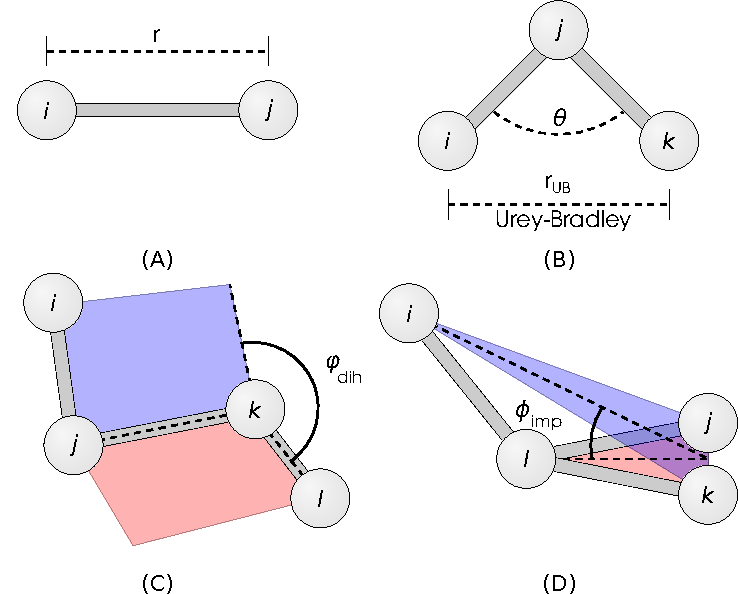
\includegraphics[width=10cm]{figures/bonded_interactions.pdf}
	\end{center}
	\captionsetup{singlelinecheck = false, justification=raggedright}
	\caption[The Bonded Interactions Calculated In Classical Forcefields]{\textbf{The Bonded Interactions Calculated In Classical Forcefields.}}{
	(A) The energy of Bond Stretching is approximated as a harmonic oscillator with respect to their separation $r$. (B) Angles between neighbouring covalently bonded atoms are also approximated as a harmonic oscillator with respect to the angle $\theta$. In some forcefields such as CHARMM there is a correction term for these angular interactions known as Urey Bradley forces. This is calculated using the separation between the non-bonded atoms $i$-$k$ in the triplet with the parameter $r_{UB}$. (C) The dihedral angle between four atoms is calculated by constructing two planes. Each plane is constructed to contain three of the four atoms in the set. One plane encompasses atoms $i, j$ and $k$ here colored in blue and the other plane contains the $j$, $k$ and $l$ atoms colored in red. The dihedral angle is then calculated by taking the angle between these two planes along the line they intersect, the line formed by the $j$-$k$ bond. (D) The improper dihedral angles enforce the planarity of a molecular configuration. A plane is constructed to contain the $i$, $j$ and $k$ (blue) atoms and another plane is constructed to contain the $j$, $k$ and $l$ atoms (red). The improper angle is then calculated as the angle between these two planes. }
	\label{charmm_bonded}
\end{figure}

\subsubsection{Non Bonded Interactions}

The term $U_{non-bonded}$ captures interactions which arise when atoms are not covalently bound to each other. Namely, Coulomb forces due to electric charges on the atoms, attractive Van Der Walls interactions and repulsion due to Pauli Exclusion,
\begin{equation}\label{nonbonded_eqs}
	\begin{aligned}
		U_{non-bonded} = \underbrace{\sum_{i>j} \epsilon_{ij} \Big( \Big(\frac{\sigma_{ij}}{r_{ij}}\Big)^{12} - \Big(\frac{\sigma_{ij}}{r_{ij}}\Big)^{6} \Big)}_{U_{Lennard-Jones}} - \underbrace{\sum_{i>j} \frac{q_i q_j } {r_{ij}}}_{U_{coulomb}}. 
	\end{aligned}
\end{equation}

Note how the repulsive Pauli Exclusion and attractive dispersion forces have been combined into one term known as the Lennard-Jones potential or $U_{LJ}$. The $\sigma$ parameter denotes the location of the local minima in the Lennard-Jones potential. This is the optimum distance that two atoms will rest against each other in the absence of other effects. The $\epsilon$ parameter denotes the depth of the potential well, or how stable the two atoms will be in the minimum energy configuration. This is very important for certain physical parameters such as osmotic pressure \cite{yoo2018}.

Meanwhile, the partial charge assignments $q_i$ for each atom are very important in a biological context, for stability of protein conformations of salt bridges and the solvation energy of different molecules \cite{jambeck2013}.

By focussing on adjusting the charges of an atom to fit the solvation energy of a molecule and adjusting the Lennard-Jones parameters to fit the osmotic pressure measurements, we  can isolate and determine these non-bonded parameters fairly well.

\begin{figure}
	\begin{center}
	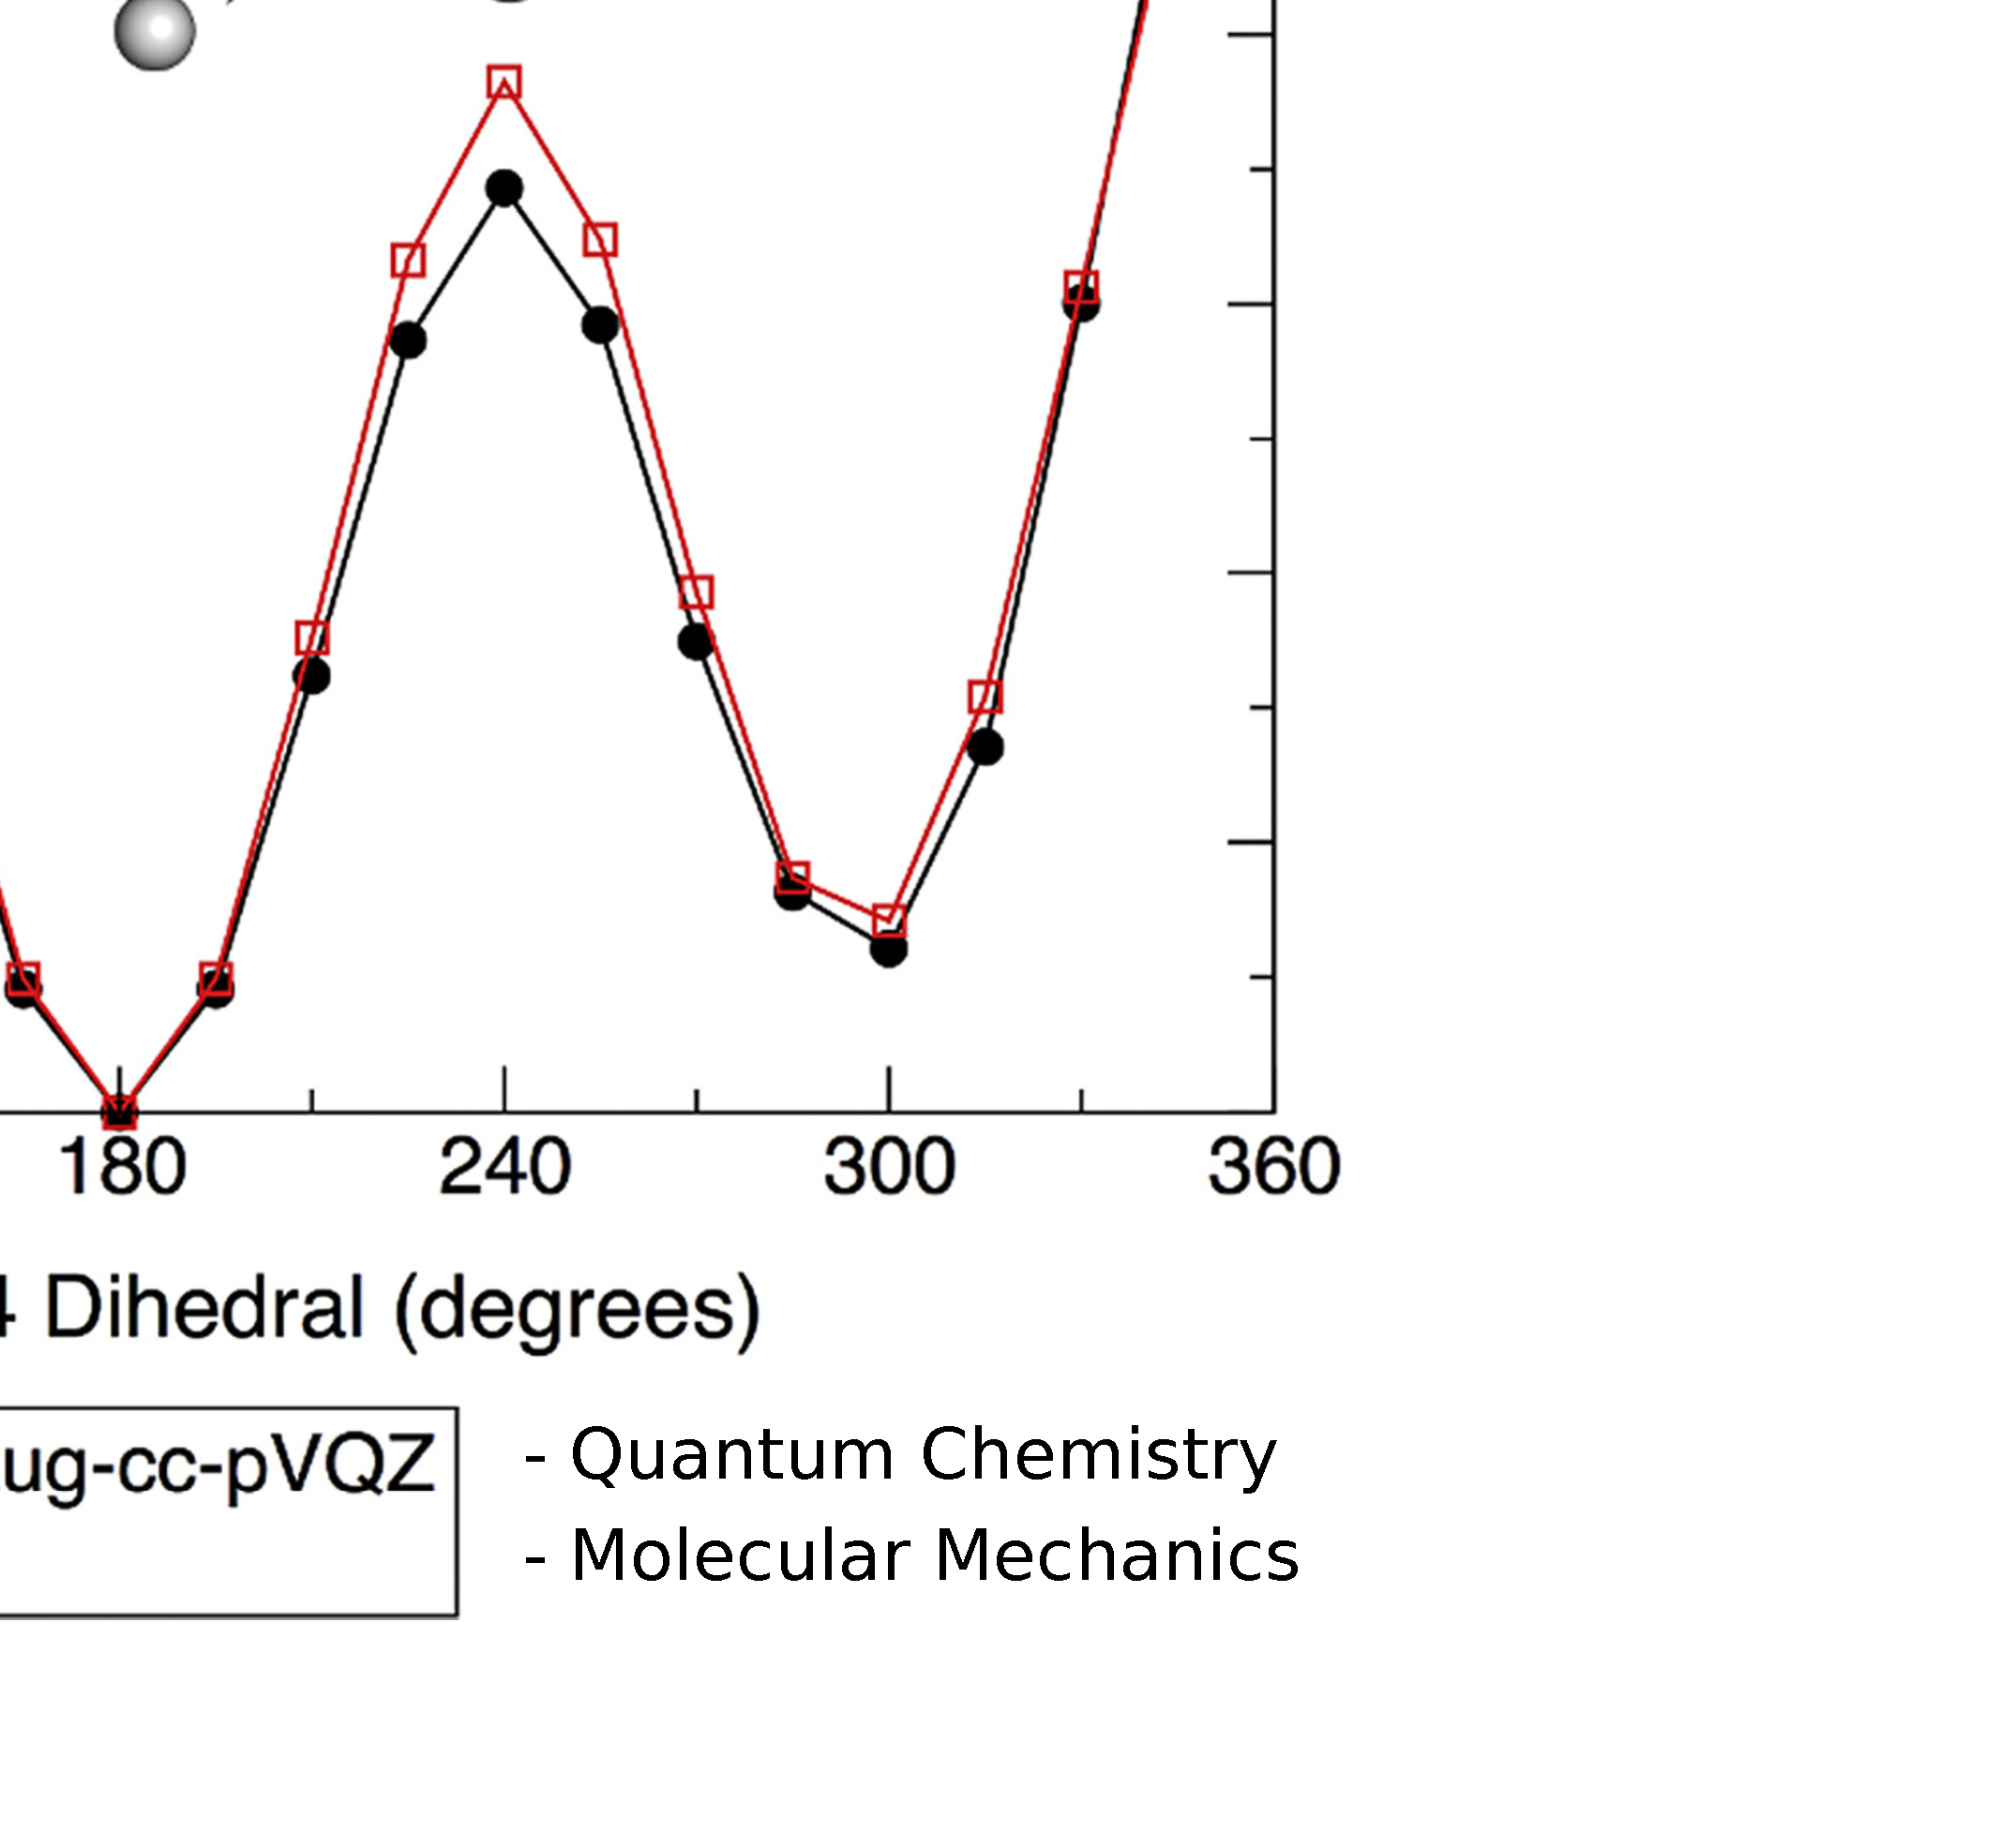
\includegraphics[width=\textwidth]{figures/QM_MM_compared.pdf}
	\end{center}
	\captionsetup{singlelinecheck = false, justification=raggedright}
	\caption[Comparison Between Potentials in Quantum and Classical Forcefields] {\textbf{Comparison Between Potentials in Quantum and Classical Forcefields}}{ A) The Morse potential was formulated to approximate the potential energy surface associated with the stretching of covalent bonds (blue). At low temperatures (the ground state, $v=0$) like those found in classical MD there is good agreement between the Morse potential and the harmonic oscillator (green) (Credit, Mark Somoza 2006). B) Here the potential of the dihedral angle between the atoms C1,C2,C3 and C4 in a butane molecule is calculated using two methods: Quantum Chemical calculations and approximations using the functional form in equation \ref{bonded_eqs} \cite{lemkul2020}. Note how the appropriate choices of $k_\varphi$, $n$ and $\delta$ have closely approximated the results in the more accurate quantum mechanical calculations.}
 
	\label{QM_MM_compared}
\end{figure}

\begin{figure}
	\begin{center}
		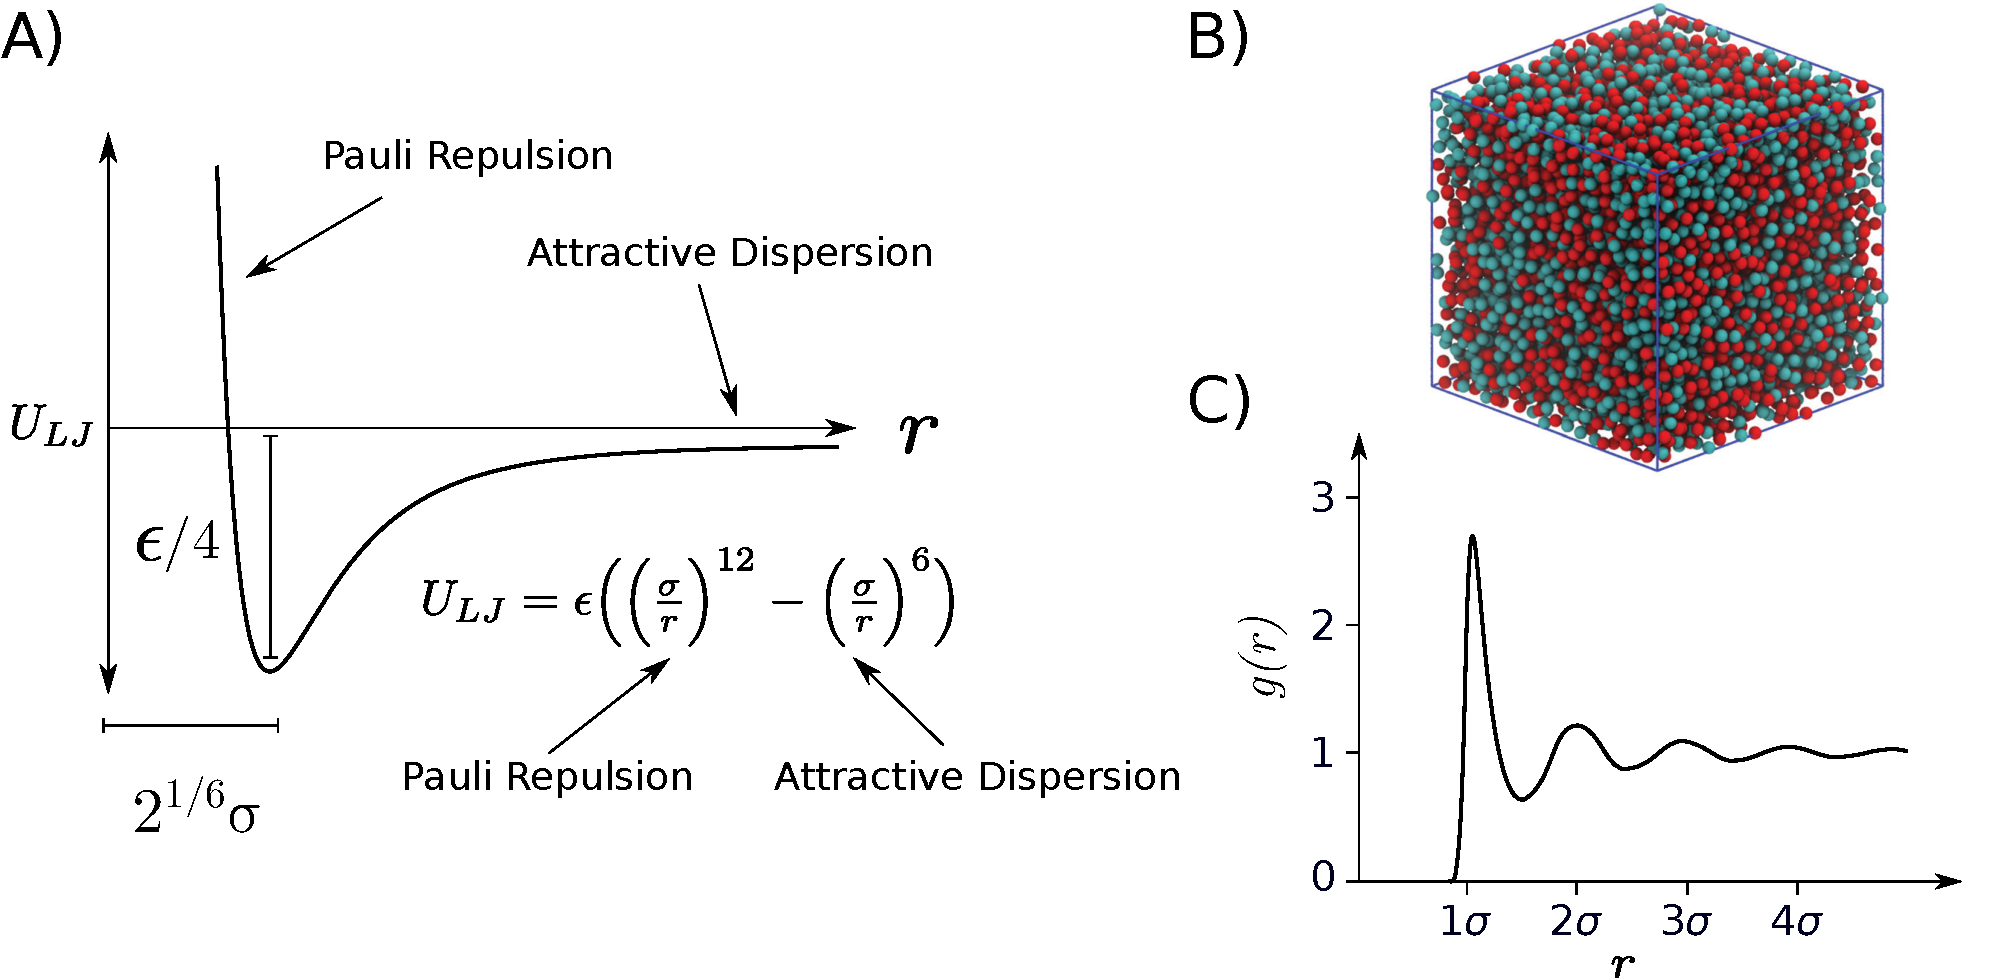
\includegraphics[width=\textwidth]{figures/LJ_figure.pdf}
	\end{center}
	\captionsetup{singlelinecheck = false, justification=raggedright}
	\caption[The Lennard-Jones Potential] {\textbf{The Lennard-Jones Potential}}{A) The Lennard-Jones potential function has two regimes, the far region one dominated by attractive dispersion forces and the close region dominated by repulsion. In the case of atomic systems this is due to the Pauli exclusion principal. B) An example of a fluid modelled with Lennard-Jones particles \cite{chari2019}. C) The radial distribution function ($g$) for a Lennard-Jones fluid \cite{morsali2005}. Note that the peaks in the distribution are spaced roughly 1 $\sigma$ apart. }
	\label{Lennard-Jones_figure}
\end{figure}

\subsection{Philosophy of Different Molecular Mechanics forcefields.}
\label{forcefields_review}
At the time of writing, the four popular forcefields for the simulation of biomolecules are CHARMM, AMBER, GROMOS and OPLS. Each of these have a slightly different philosophy in their formulation. They may be bottom up, as in the case of AMBER and CHARMM or top down, in the case of OPLS. Bottom up forcefields take the results from \textit{ab initio} MD calculations as an initial guess and approximate them by tweaking the parameters in the functional form in equation \ref{CHARMM_effective_potential_eq}. Conversely, top down forcefields tweak these parameters with reference to experimental measurements. Ultimately, the results from \textit{in silico} experiments must match those of wet lab experiments, so the development of all forcefields has elements of both philosophies. All forcefields assign the partial charges to atoms using the results of \textit{ab initio} MD calculations. The rest of the parameters are derived with other methods such as attempting to match the known secondary structures of peptides \cite{huang2016}. Different forcefields have different methods of deriving their parameters. Below is a short summary of the philosophy for the four major forcefields taken from the review by Justin Lemkul \cite{lemkul2020}. 

\begin{itemize}
	\item CHARMM: The most popular all atom forcefield. To build CHARMM, QM optimized geometries and molecular dipole moments are compared to those found from calssical MD simulations. Molecular degrees of freedom such as dihedral angles are also fit with QM energy profiles, an example can be seen in \ref{QM_MM_compared}. Macroscopic experimental quantities are also used to validate the parameters in this forcefield, such as solvation energies, crystal geometries, heats of vaporization and conformational sampling of biomolecules \cite{huang2016}. One of the reasons for this forcefield's popularity is its considerable library of supported compounds, especially when combined with its generalisation module CGENFF \cite{vanommeslaeghe2010}. 

	\item AMBER: An all atom forcefield which is built from the ground up from results from quantum mechanical calculations and results from spectroscopy. A version of this forcefield has become the favorite for the simulation of disordered proteins \cite{robustelli2022, robustelli2018}. There is also a generalised version of the AMBER forcefield known as GAFF \cite{wang2004, wang2006}. Comparisons between generalised forcefields can be found in \cite{zhu2019}.

	\item OPLS: An all atom forcefield. The OPLS forcefield takes the philosophy that, since many biomolecules share similar geometries to certain organic liquids, biomolecules can be accurately parameterised by creating a forcefield which correctly reproduces the experimental measurements for these species. Parameters are derived to accurately reproduce the liquid density of certain organic liquids. These parameters are then used as roots to construct larger biomolecules by drawing analogies between similar molecular geometries. 

	\item GROMOS: A united atom forcefield, where hydrogen atoms are typically merged into the heavy atom they are bound to. Hence, they are not explicitly treated. Charge assignment is done with DFT. Interestingly, GROMOS uses a quartic form of the bond stretching term 
		\begin{equation}
			U_b = \frac{1}{4} k_b (b^2-b^2_0)^2.
		\end{equation}

		The parameters are adjusted for agreement with experimental values such as  solvation energies, liquid densities. GROMOS forcefields are popular in some contexts because of its ability to reproduce partition coefficients between polar and non-polar media, a similar chemical context to what is found at the interface between a membrane and bulk water.

\end{itemize}

\section{Periodic Boundaries To Pretend A Protein is Inside a Cell}
\begin{figure}
	\begin{center}
		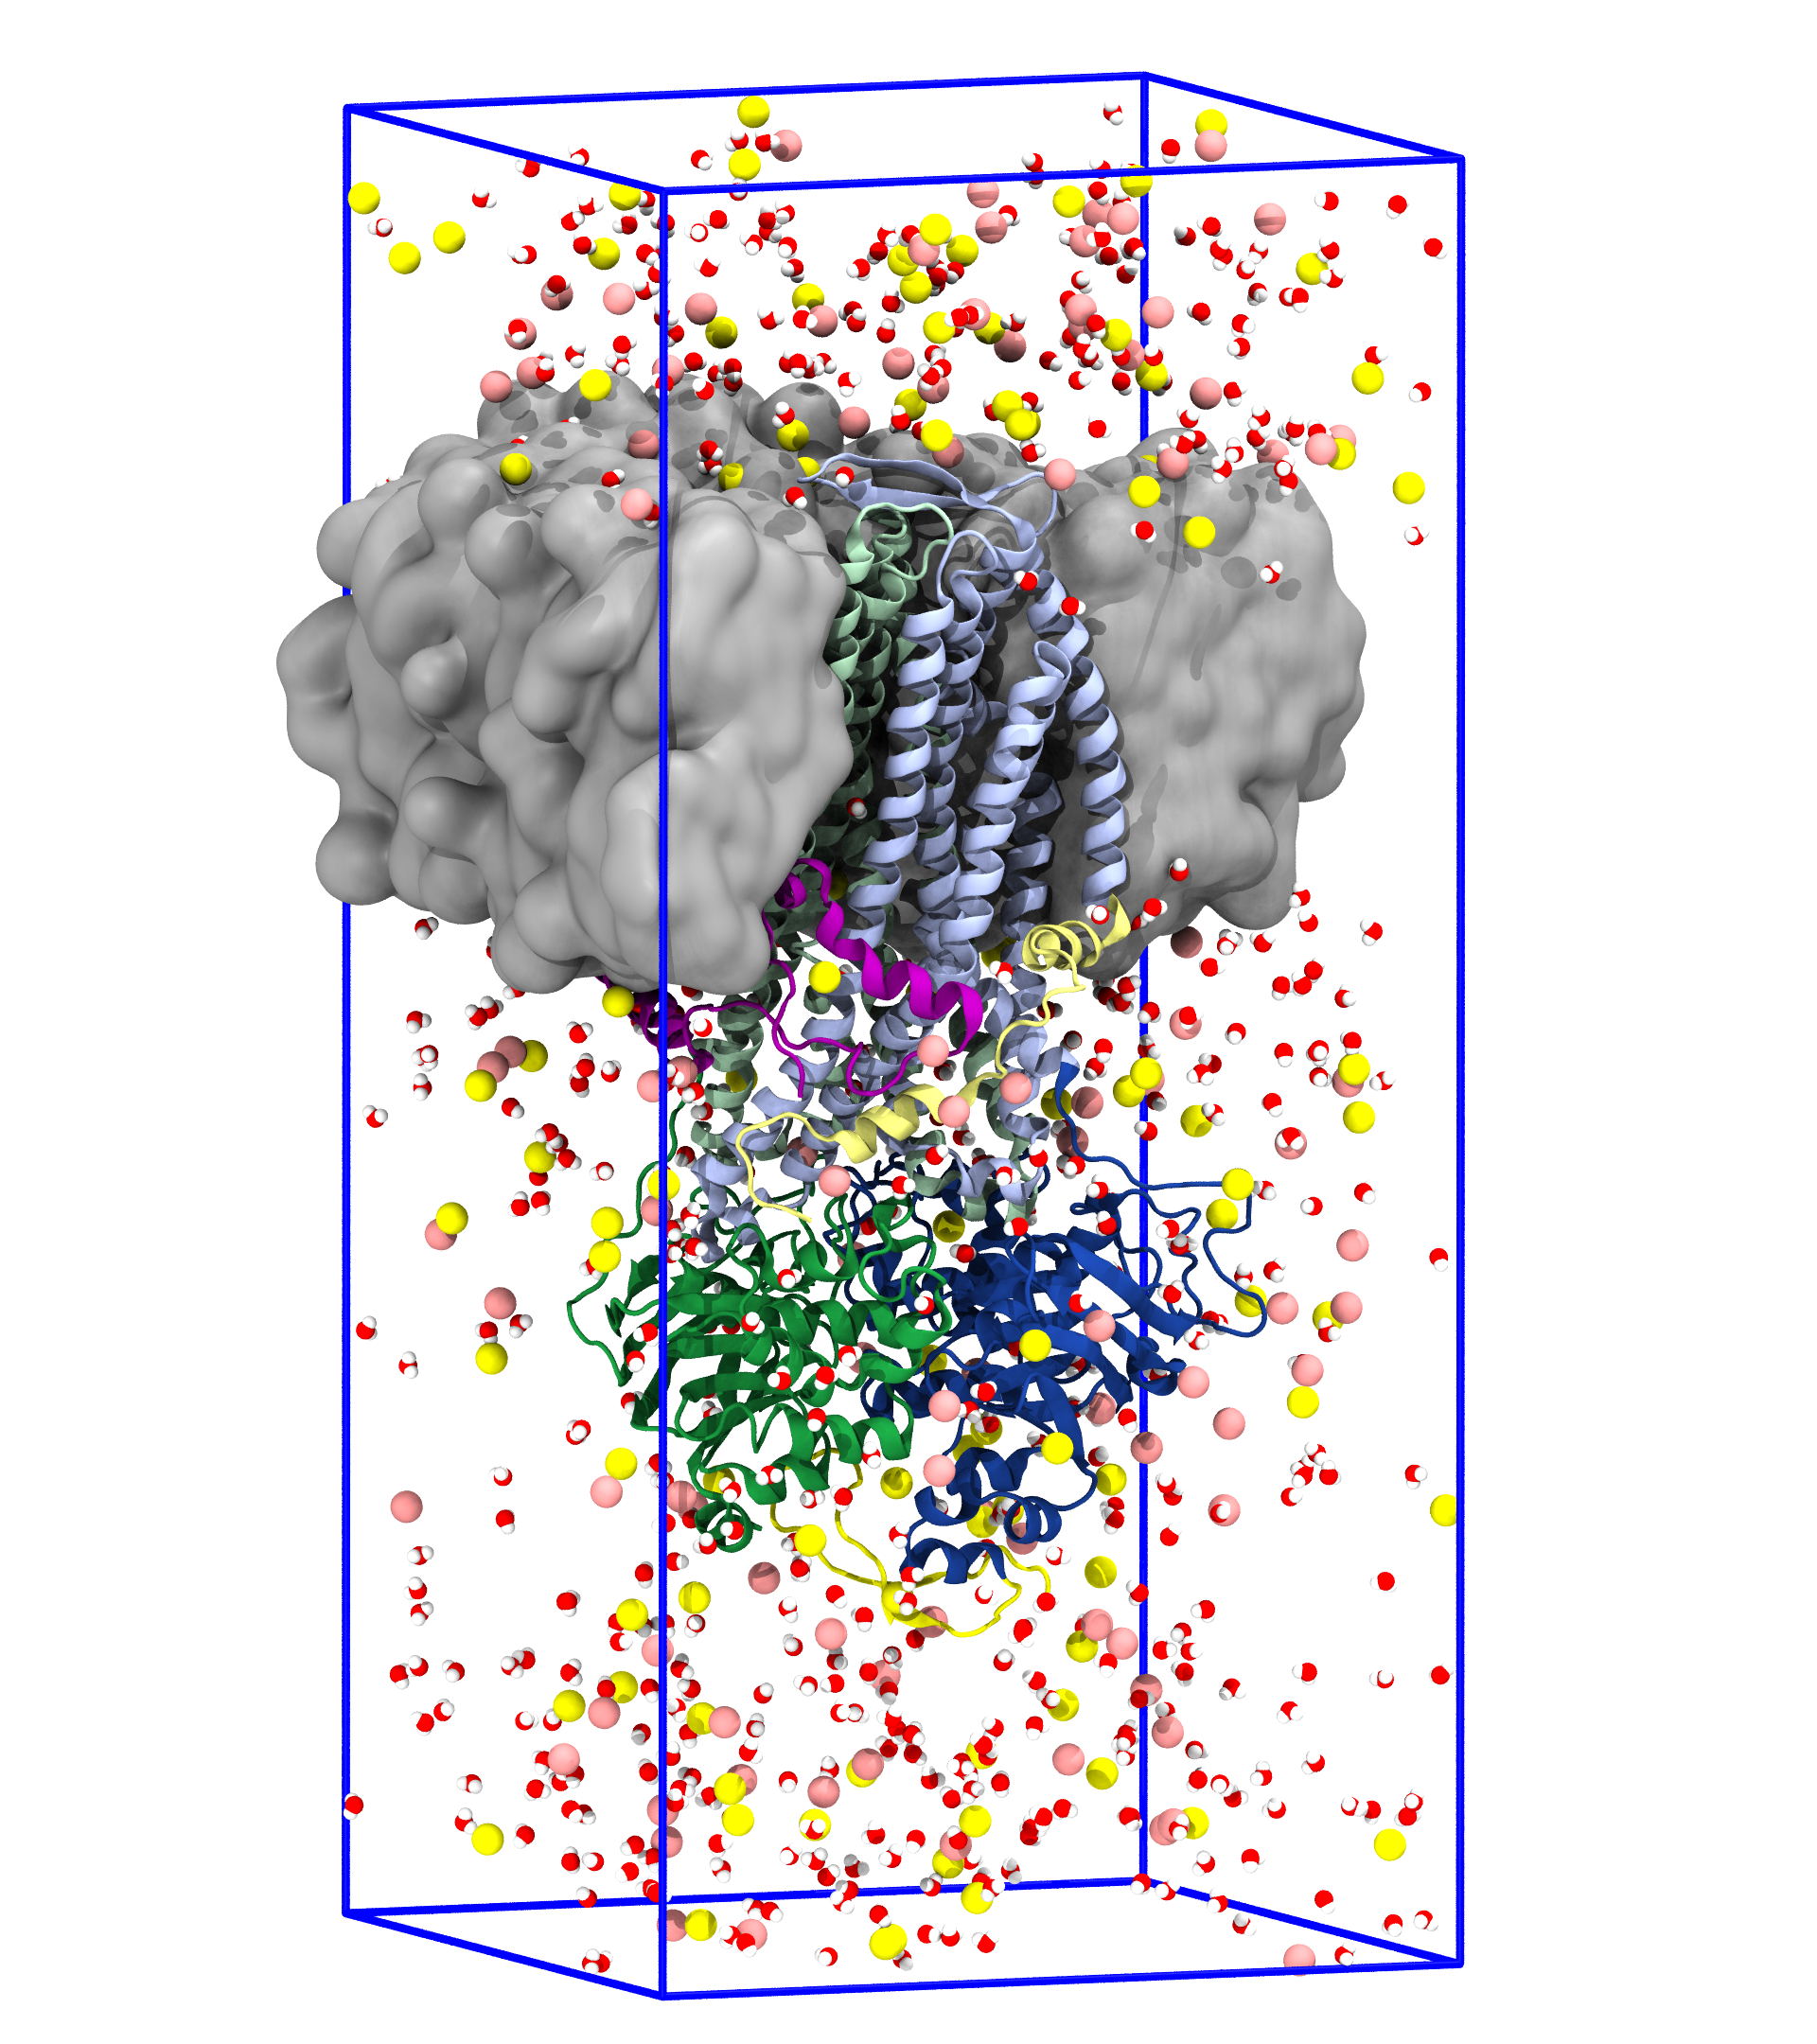
\includegraphics[width=\textwidth]{figures/MD_unit_cell_example/MD_system.png}
	\end{center}
	\captionsetup{singlelinecheck = false, justification=raggedright}
	\caption[An Example of a Solvated Biomolecular Environment Ready for Simulation] {\textbf{An Example of a Solvated Biomolecular Environment Ready for Simulation}}{This rendering shows a CFTR protein embedded in a lipid bilayer, immersed in a potassium chloride solvent. Half of the bilayer has been stripped away, as has much of the solvent so the protein is visible. The phospholipid lipid bilayer is colored grey, while the potassium chloride ions are colored pink and yellow, respectively. Water molecules are red and white. The blue box indicates the boundaries of the unit cell. This system contains roughly 190,000 atoms in total.}
	\label{MD_environment}
\end{figure}

Inside cells, proteins are immersed in a large solvation environment composed of water and salts \cite{phillips2012}. An example can be seen in figure \ref{MD_environment}. However, simulating such a large environment is computationally expensive and truncating it with vacuum at the boundaries leads to water molecules aligning their dipole moments along the boundary and perturbing equilibrium dynamics. In order to avoid such artefacts, we have to replicate the large cellular environment somehow \cite{ross2018}. We could make a simulation box large enough to replicate the behavior of a bulk solvent, but even with a large simulation box we can still observe artifacts associated with the vacuum at the boundaries \cite{gapsys2020}. So, to avoid these boundary effects, we use periodic boundary conditions (PBCs), allowing atoms to move between images in the simulation box. This replicates the molecular system infinitely in every direction. 

Using PBCs might remove vacuum from our molecular system but now we have a different problem. Effectively, with the PBCs, we have created a system with an infinite number of atoms. We have to somehow limit the number of computations we perform. We could simply truncate the calculation of interactions $U_{non-bonded}$ after a certain cutoff distance. This is not an issue for $U_{LJ}$ because the $1/r^6$ and $1/r^{12}$ terms in equation \ref{Lennard-Jones_figure} decay very quickly for large $r$. Inaccuracies due to this approximation can be further ameliorated with the use of a smooth switching function \cite{klauda2007, venable2009}. On the other hand, the $1/r$ dependence in $U_{coulomb}$ scales much more slowly so truncating it leads to a loss of accuracy in the results of the simulation \cite{auffinger1995, perera1995, roberts1994, delbuono1996, essmann1995}. So, we have to calculate the contributions of $U_{coulomb}$ in between all periodic images. Note that this periodicity requires that the unit cell is electrically neutral, else the contribution of potential energy from $U_{coulomb}$ will be infinite, leading to artefacts \cite{hub2014}.

\begin{figure}
	\begin{center}
		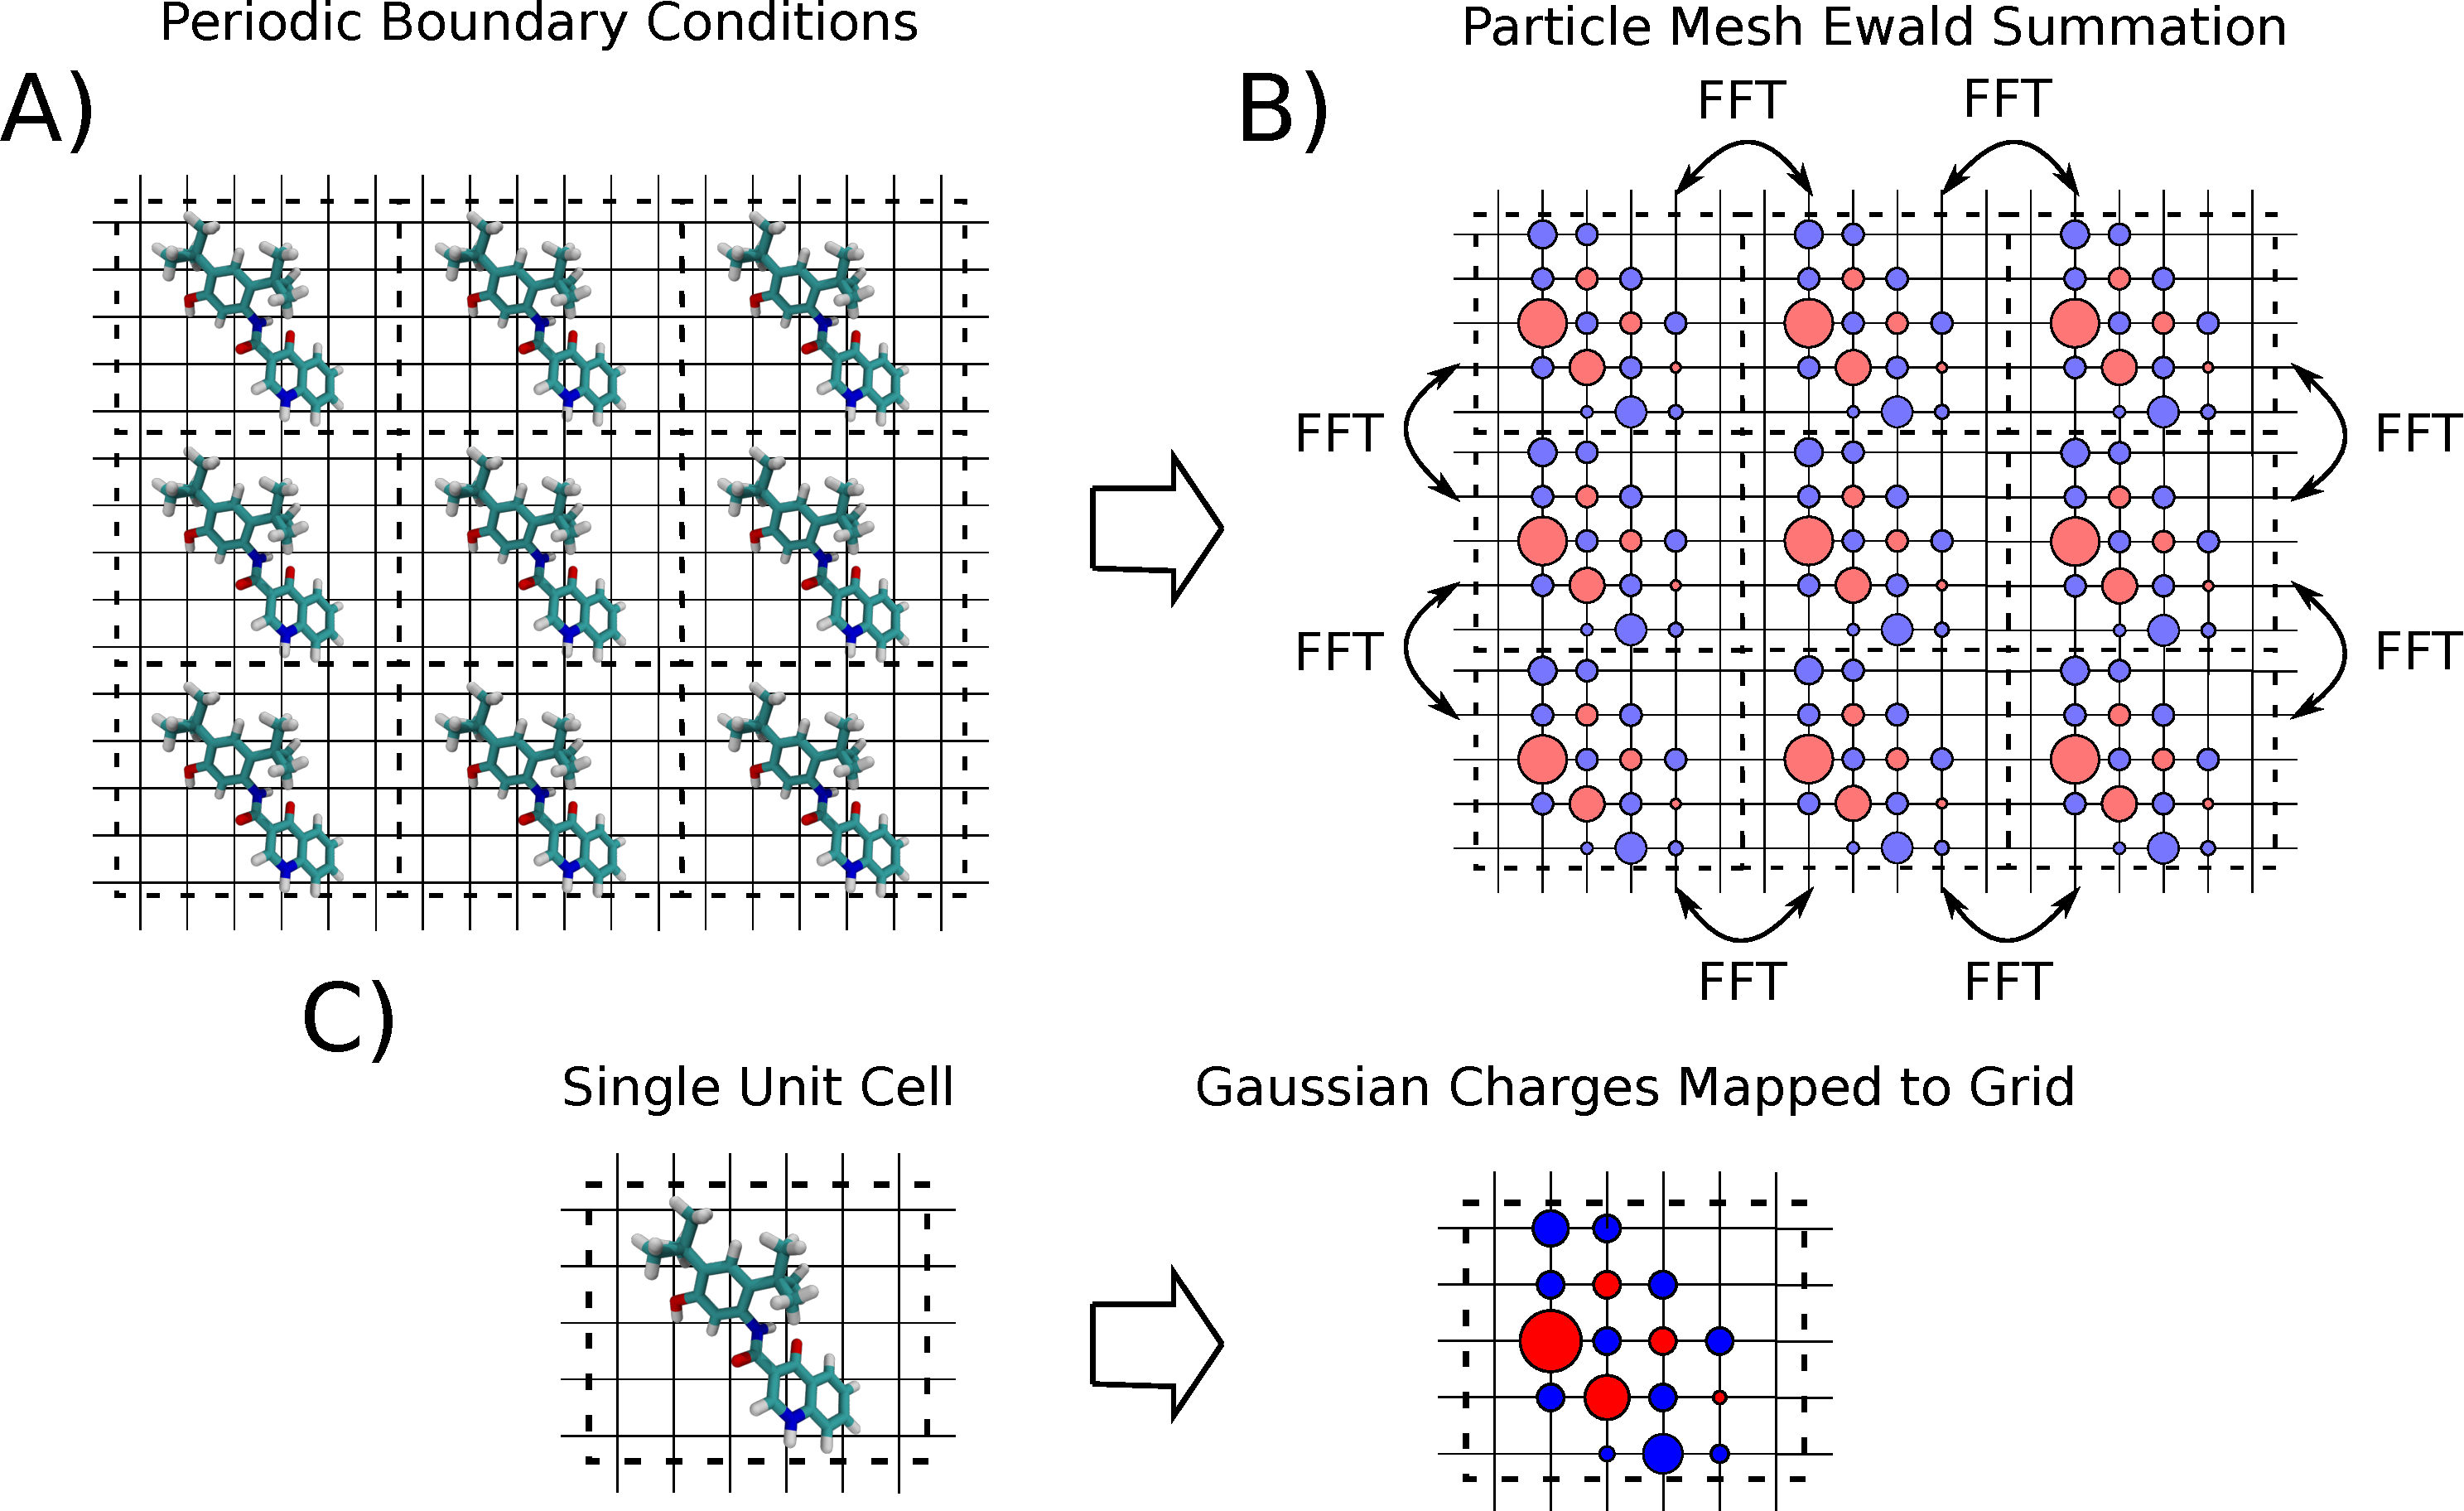
\includegraphics[width=\textwidth]{figures/PME_miro.pdf}
	\end{center}
	\captionsetup{singlelinecheck = false, justification=raggedright}
	\caption[Particle Mesh Ewald Summation] {\textbf{Particle-Mesh Ewald Summation}}{A)The molecular system is repeated infinitely along all axes, when atoms reach the edge of the simulation box, they are allowed wrap around to the other side of the box. B) The charges in the infinite periodic system are approximated onto a regular grid. Then the potential in the infinite system is calculated via a Fast Fourier Transform (FFT). C) A more detailed view of the charge mapping procedure. The charges in the system are interpolated onto the grid using B-spline interpolation. }
	\label{PME_illustration}
\end{figure}

To calculate $U_{coulomb}$ in all periodic images and limit computational intensity of our calculations we use a clever scheme known as Particle-Mesh Ewald summation (PME). Interestingly, this scheme ends up scaling better than the pairwise summation in equation \ref{nonbonded_eqs} might imply. The direct summation scales with computational complexity of $O(N^2)$  with the number of atoms while the infinite PME scheme scales as $O (N\log N)$ \cite{darden1993}, though there are some further considerations for large systems on parallel architectures \cite{hardy2015}. Even with these sophisticated algorithms, the calculation of electrostatic potential in the infinite system still represents the largest computational bottle-neck in classical MD \cite{hardy2015}.

For a detailed review of different Particle-Mesh Ewald summation methods and the mathematics behind the method see \cite{shan2005}. A brief outline of the Smooth Particle Mesh Ewald summation is given below 

\begin{enumerate}
	\item An \textit{ansatz}  is used where $U_{coulomb}$  has Gaussian screening charges added to it and simultaneously subtracted away to create a smooth potential. The details can be found in \cite{shan2005}.
		\begin{equation}
			\begin{aligned}
			U_{coulomb} &= U_{screening-charges} + U_{coulomb}  - U_{screening-charges}.
			\end{aligned}
		\end{equation}
		Terms in these equations are then rearranged such that one term is evaluated with a Fourier transform and the other term is evaluated using a direct sum.
		\begin{equation}
			\begin{aligned}
			U_{coulomb} &= U_{FT}  + U_{direct-sum}.
			\end{aligned}
		\end{equation}
	\item The charges to be evaluated using $U_{FT}$ are interpolated onto a grid using B-spline interpolation functions. This is the procedure demonstrated in figure \ref{PME_illustration}.
	\item The charge density functions for the charges on the grid are transformed into frequency space using Fast Fourier Transforms.
	\item The Poisson equation is solved numerically in frequency space for these charges.
		\begin{equation}	
			\nabla^2\tilde{U} = 4\pi \tilde{\rho}(\bold{k})
		\end{equation}	
		Where $\tilde{U}$ is the component of $U_{FT}$ we solve for in frequency space and $\tilde{\rho}$ is the Fourier transform of the smooth scalar function for the interpolated charge densities. 
	\item An inverse Fourier transform is calculated for the solution to $\tilde{U}$ to transform it back into real space. 
	\item The interactions in $U_{direct-sum}$ are evaluated using a simple pairwise summation.
	\item Now that $U_{coulomb}$ is known at every position in the unit cell, we can move atoms according to the contributions from this potential using Newton's second law.
\end{enumerate}

\section{Controlling the Temperature and Pressure in a Simulation}
Living things are very sensitive to their external environment. Enzymes only work in a narrow range of temperatures and cells burst apart in the absence of pressure\cite{peterson2007, song2012}. As such, to correctly understand biological systems we not only need to simulate the dynamics of the atoms inside them, but we must also make sure that the virtual environment in our simulations matches what is found inside cells or in the laboratory. Our simulations should seek to approximate the environment of an open topped test-tube sitting in a pressure and temperature controlled laboratory. To do this, we make use of some statistical ensembles chosen for their performance in regulating the thermodynamic quantities in a simulation and their computational expense.  

%Langevin dynamics
%\begin{equation}
%	m_i  \dot{v} _i = F_i + m_i \gamma_i \bold{v}_i + R(t)
%\end{equation}

\subsection{Hot and Cold with the Nos\'e-Hoover Thermostat}
Recall that the temperature of a system is a direct function of the velocity of its constituent particles. So by regulating the ensemble of velocities we can control the temperature. We begin a simulation by choosing the velocities of the atoms within the system from a Maxwell-Boltzmann distribution 

\begin{equation}
	f(v_i) = \Big(\frac{m_i}{2\pi k_B T}\Big)^{3/2} \exp{\Big(-\frac{m_iv_i^2}{2k_BT}\Big)},
\end{equation}

where $f(v_i)$ is the proportion of particles with velocity $v_i$, $k_B$ is Boltzmann's constant. Note that $i=1,...,N_{df}=3N$ as we choose a velocity component for $x,y \ \text{and}\  z$ separately. 

Despite starting from the same Cartesian coordinates, randomly sampling velocities from the Maxwell-Boltzmann means that replicate simulations will immediately begin from different points in phase space. Their coordinates will quickly diverge, raising questions around how long one should run a simulation and how many replicates they should run in order to collect reliable statistics. According to Knapp et al. \cite{knapp2018}, a good rule of thumb is to simulate between 5 and 10 replicates depending on the availability of computing resources\footnote{Recall that in the ergodic limit, a quantity $f$ calculated from the ensemble average of replicates will be equal to the time average calculated from one replicate in the limit $t\to\infty.$ That is $$ \langle f \rangle_i = \lim_{t \to \infty } \frac{1}{t} \int_0^tf(\tau)d\tau $$}. In this thesis we prioritised long time scales to sample slow motions, so 3 replicates with run times between 1 and 2 microseconds were produced for all systems. 

After the initial choice of velocities, the temperature in a simulation is maintained by directly modulating the velocities of the atoms to maintain the target temperature $T_0$. There are many schemes which attempt this. We will discuss the Nos\'e-Hoover thermostat in detail here because it was used during the production runs in this thesis  \cite{nose1984, hoover1985, martyna1992}. However, for the equilibration phase of the simulations, we used the Berendsen thermostat because it is faster at correcting large temperature differentials but does not produce the correct statistical ensemble \cite{bussi2007, berendsen1984}. We also note that the field has since moved on to favor the Bussi thermostat, which is an extension of the Berendsen thermostat, as it works well in most contexts  \cite{bussi2007, braun2019}.

The Nos\'e-Hoover thermostat is characterised by the use of an extra, massive particle coupled to an external bath. The use of a single bath has been associated with issues with ergodicity and so usually this particle is coupled to a chain of external baths. Usually, the software simulation package GROMACS uses a chain of 10 baths, $M=10$ \cite{martyna1992, martyna1996, abraham2015}. The Hamiltonian for the Molecular Dynamics system coupled to a chain of $M$ external baths is then

\begin{equation}
	H_{NH} (\bold{x},\bold{p},\eta_1 , ... , \eta_M, p_{\eta_1}, ...,  p_{\eta_M}  )= H_{MM} + \sum_j^M \frac{p^2_{\eta_j}}{2Q_j} +k_BT  N_{df}   \eta_1   + k_BT \sum_{j=2}^M\eta_j.
\end{equation}

Here, usually $N_{df} := 3N$ unless there are constraints placed within the system to freeze atoms. $\eta$ denotes the 1 dimensional coordinate of the thermostat particle with mass $Q$, while $H_{MM}$ is the Hamiltonian of the unregulated molecular mechanics system 

\begin{equation}
H_{MM}(\bold{x},\bold{p}) = \underbrace{\sum_i^N \frac{\bold{p}_i^2}{2 m_i}}_{E_{kinetic}} + U_{CHARMM} (\bold{x}). 
\end{equation}

By using Hamilton's equations of motion, $H_{NH}$ evolves by

\begin{equation}
	\begin{aligned}
		\dot{\bold{x}_i} &= \bold{p}_i/m_i \\
		\dot{\bold{p}_i} &= \bold{F}_i-\bold{p}_i\frac{p_{\eta_1}}{Q_1} \\
		\dot{\eta_j} &= p_{\eta_j}/Q_j \\
		\dot{p_{\eta_1}} &= \bigg[\sum_i^N \frac{\bold{p}_i^2}{m_i} - N_{df} k_B T\bigg]  - p_{\eta_1}\frac{p_{\eta_2}}{Q_2} \\ 
		\vdots \\ 
		\dot{p_{\eta_j}} &= \bigg[ \frac{p^2_{\eta_{j-1}}}{Q_{j-1}} - k_bT \bigg]  - p_{\eta_{j}}\frac{p_{\eta_{j+1}}}{Q_{j+1}} \\ 
		\vdots \\ 
		\dot{p_{\eta_M}} &= \bigg[ \frac{p^2_{\eta_{M-1}}}{Q_{M-1}} - k_bT \bigg],
	\end{aligned}
	\label{NH_equations}
\end{equation}
where $\bold{F}_i$ is the force vector on the $i$th particle. It may be calculated from $U_{CHARMM}$ using Newton's second law. 

The parameters $Q_j$ are chosen by the user to control the coupling strength of the baths to each other. We usually choose   
\begin{equation}
	Q_j = \frac{\tau_{NH}T_0}{4\pi^2}\qquad  \forall j,
\end{equation}
where $\tau_{NH}$ is the time interval between when the thermostat parameters are updated. This means that whenever the simulation is not at a time step that is a multiple of $\tau_{NH}$,  we can just evaluate $U_{CHARMM}$ as normal but every interval of $\tau_{NH}$, we rescale the velocities according to the equations of motion in \ref{NH_equations} to match the correct temperature $T$.

Remember that we can always calculate the temperature using the instantaneous velocities in the simulation using

\begin{equation}
	\begin{aligned}
		T &= \frac{2E_{kinetic}}{3Nk_B}  =  \frac{\sum_i m_i v_i^2}{3Nk_B} 
	\end{aligned}
\end{equation}
	
The Nos\'e-Hoover thermostat, when chained infinitely, allows us to  accurately produce what's known as an NVT ensemble, also called the canonical ensemble in the statistical mechanics literature \cite{martyna1992}. Where the number of particles in the system (N) remains constant, the volume of the system remains constant (V) and the temperature remains constant (T). In a realistic environment, the pressure remains constant rather than volume, so we need another regulatory mechanism to modulate the volume of the system to regulate the pressure (P) and produce an NPT ensemble. 

\subsection{Under Pressure with the Parinello-Rahman Barostat}
Pressure is critical to the function of living organisms. Membranes burst apart at low pressures \cite{karal2021} and at high pressures cellular function is disrupted \cite{macdonald2001}. In order to accurately reflect the atmospheric pressure at which living things thrive we have to accurately calculate and modulate it during our simulation.

In order to measure the pressure at the simulation walls, we follow the procedure in \cite{allen1991} by calculating a quantity known as the virial:

\begin{equation}
	W(\bold{x}) = \sum_i^{N-1} \sum^N_{j>i} \bold{r}_{ij} \cdot \bold{F}_{ij},
\end{equation}

where $\bold{r}_{ij} = \bold{x}_i - \bold{x}_j$  is the Cartesian distance between the $i$th and $j$th atoms, while $\bold F_{ij}$ is the force extorted on atom $j$ by atom $i$. 
This is then substituted into the equation 

\begin{equation}
	P (\bold{x}) = \frac{N k_B T + \langle W \rangle_i}{V}
	\label{instantaneous_pressure}.
\end{equation}

And so using equation \ref{instantaneous_pressure}, we can modulate the volume $V$ of the simulation in order to control the pressure throughout the simulation.

For this purpose, we apply the Parrinello-Rahman barostat \cite{parrinello1980, parrinello1981}, using a procedure with a similar philosophy to the extended Hamiltonian used in the Nos\'e-Hoover thermostat. In this case, the system is coupled to an external pressure bath rather than an external temperature bath. First we define that the basis vectors for the periodic simulation box as $\underline{h}:= [\bold{a}, \bold{b} ,\bold{c}]$. When the box is scaled to change the volume these basis vectors are multiplied by a set of scalars $s_i := (\xi_i$, $\eta_i, \zeta_i ) \in [0,1]$. We perform a change of coordinates so that the contributions of the particles onto the boundaries is easily calculated from our equations so we express the atomic coordinates as

\begin{equation}
\begin{aligned}
	\bold{x}_i &= \xi_i \bold{a} +\eta_i \bold{b} +\zeta_i \bold{c}  \\
	           &= \underline{h}\bold{s}_i.
\end{aligned}
\end{equation}

Defining $\underline{G} := \underline{h}^T\underline{h}$, the Lagrangian for the scaling system then becomes
\begin{equation}
\begin{aligned}
	L = \frac{1}{2} \sum_i^N \  m_i \dot{\bold{s}}_i^T\underline{G}\dot{\bold{s}}_i - \sum_i \sum_{j > i } \phi (\bold{r_{ij}}) + \frac{1}{2} \ M \text{Tr}(\dot{\underline{h}}^T\dot{\underline{h}})   - {P}_{ext} V,
\end{aligned}
\end{equation}

where $\phi(\bold{r}_{ij}$ is the pairwise potential between two atoms in $U_{CHARMM}$, while $M$ is a constant of proportionality associated with the kinetic energy derived from the movement the particles undergo as they scale. It has units of mass. $P_{ext}$ is our target, externally applied pressure. This Lagrangian allows us to derive the equations of motion  

\begin{equation}
\begin{aligned}
	\ddot{\bold{s}}_i &= -\sum_{j\neq i}   \frac{1}{m_i\bold{r}_{ij} }\frac{d\phi(\bold{r}_{ij})}{d r_{ij}}  (\bold{s}_i - \bold{s}_j) - G^{-1}\dot{G} \dot{\bold{s}}_i \\
	\ddot{\bold{h}} &= \frac{1}{M} (\bold{Y} -P_{ext}) \underline{\sigma}.
\end{aligned}
\end{equation}
The matrix $\underline{\sigma} := V (\bold{h}^T)^{-1} = V  [\bold{b} \times \bold{c}, \bold{c} \times \bold{a}, \bold{a} \times \bold{b}] $  contains information about the size and orientation of the simulation box, while 

\begin{equation}
\begin{aligned}
	\bold{Y} = \frac{1}{V}\sum_i m_i (\underline{h}\dot{\bold{s}}_i) (\underline{h}\dot{\bold{s}}_i)^T + \sum_i \sum_{j>i}\frac{1}{{r}_{ij}} \frac{d \phi (\bold{r}_{ij})}{dr_{ij}} \bold{r}_{ij}\bold{r}_{ij}^T,
\end{aligned}
\end{equation}

represents the stress tensor which acts across each of the faces of the unit cell. 
This system of equations can be solved numerically to control the pressure of the simulation system by modulating the length of the basis vectors $\bold{a}, \bold{b}$ and $\bold{c}$ contained in $\underline{h}$.

	Together with the Nos\'e-Hoover thermostat, the Parrinello-Rahman barostat produces NPT, also called the isothermal-isobaric ensemble in the statistical mechanics literature. The combination of these two methods is thus appropriate for simulating a cellular environment. 


	\section{The Process of Preparing an MD Simulation}
	The process of taking a molecular structure and putting it in a cellular environment to simulate it at physiological temperatures is both an art and a science. It's a science because a biophysicist must be aware of the many tricks that structural biologists use to image a macromolecular complex. But it's an art because accounting for those tricks and making the necessary modifications is rarely straightforward. How do you build a missing loop? What charge state is an amino acid most likely to take in a physiological context? These questions must be carefully answered by analysing the literature about the system of interest. Once the protein structure has been built, the system is immersed in a water solvation bath alongside a concentration of salt ions, usually sodium chloride if the environment is thought at be extra cellular or potassium chloride if the environment is thought to be intracellular. Once the initial conditions have been decided, we need to make a few preparatory steps so the simulation collects reasonable results and doesn't hurtle along some unphysical trajectory. The steps so that the simulation remains realistic are fleshed out in some more detail in \cite{braun2019} but we produce a short summary below.

	\begin{enumerate}
		\item Minimisation: Here the atoms are moved down along $U_{CHARMM}$ to resolve any clashes in the system which would cause LINCS or SHAKE to diverge. This is usually done with simple minimisation algorithms such as steepest descent or conjugate gradient descent \cite{leach2001}. This performed while the simulation box has a fixed volume. 
	\item Relaxation: Harmonic restraints are placed on the heavy atoms (non hydrogen) in the system so that large conformational changes do not occur while the macromolecules are heated and settle into their solvation environment. This may be done under the NVT or NPT ensembles depending on the system. Sometimes the system is heated slowly from 0 Kelvin up to the desired thermal temperature in order to avoid large conformational changes which might result from different parts of the system heating at different rates. 
\item Equilibration: Often after relaxation more simulation time is run so that the system can settle into local minima further. This process makes sure that the physically relevant local minima are being sampled once we move to production. This process could be run for a few nanoseconds or up to a microsecond. It depends on the system. This is usually done with the NPT ensemble.
\item Production: Here the NPT ensemble is applied and the system is allowed to evolve under Newton's equations of motion while data is collected for analysis.
\end{enumerate}


\section{Choosing an Appropriate Time Step}
The discrete time step, $\Delta t$ which is used to integrate our equations of motion is one of the most important determinants in the performance of the simulation. We would like $\Delta t$ to be as large as possible, so that the minimum number of calculations are made to sample the desired time scale. In the case of proteins this usually runs between $10^{-6}$ and $10^{-3}$ s \cite{robustelli2022}.  

As you can see in table \ref{timescales} the fastest motion in molecular systems is dictated by stretching of covalent bonds. Studies of the resonance of molecules by infrared spectroscopy determined that the O-H type bonds oscillate the fastest, with a resonance peak at 3600 cm$^{-1}$\cite{schlick2010}. 

Due to Nyquist's theorem the largest $\Delta t$ parameter we can choose \textit{must} be less than half the speed of the fastest degree of freedom in the system \cite{shannon1949}. However, empirically we have found that condensed matter systems require even shorter time steps to maintain their stability \cite{leach2001}. The Verlet leap-frog scheme used in most MD codes requires between 5 and 10 integration steps per period of the fastest harmonic mode in a system, to maintain stability \cite{mazur1997, feenstra1999}. The choice of too large a time step means that the system will escape local free energy minima, accumulating kinetic energy and eventually ``blow-up" \cite{braun2019}. In the case of biomolecular systems we are challenged by the fact that they are so hydrogen-rich. Since hydrogen is so light, its motion is much faster compared to the other molecular motions involving heavier, slower moving atoms. Its correlation time is on the order of 1 femtosecond. In classical simulations we are able to get away with using 2 femtoseconds with the use of specialised integration schemes such as SHAKE\cite{andersen1983} and LINCS\cite{hess1997} to constrain the fast motion of hydrogen atoms. This allows us to use $\Delta t = 2$ fs in atomistic classical MD simulations.

The use of techniques such as hydrogen mass repartitioning \cite{balusek2019}, virtual site topologies \cite{feenstra1999} and multiple time step schemes \cite{streett1978} have also gained popularity in recent years in order to increase time steps further, up to $\Delta t = 5 $fs. 

\begin{table}
	\begin{center}   
		\begin{tabular}{ |c|c|c|}
			\hline
			Motion & Timescale \\
			\hline
			Covalent Bond-stretching & $1-2\times10^{-15}$ s \\
			Covalent Bond-angle bending & $5-10\times10^{-15}$ s \\ 
			Sidechain  Motions & $10 ^{-12}-10^{-6}$ s \\
			Rigid Body Motions & $10 ^{-9}-1$ s \\
			Ion Conduction & $10^{-9}-10^{-6}$ s \\
			Protein Conformational Changes & $10^{-9}-10^{-3}$ s \\
			Alpha Helix Formation & $10^{-9}-10^{-6}$ s \\
			Beta Sheet Formation & $10^{-6}-10^{-3}$ s \\
			Protein Folding & $10^{-6}-10$ s \\
			\hline
		\end{tabular}
\end{center}
%\begin{tabular} { |c|c|c| } 
%	\hline
%	%\label{atomic_motions_speed}
%	System Description & Fastest Degree of Freedom & Characteristic Timescale \\ 
%	\hline
%	Uncoupled Atoms  & Atom Translation & 10 fs  \\ 
%	Rigid Molecules & Rigid Body Rotation & 5 fs \\  
%	Flex. Molecule with Rigid Bonds & Bond Angle Vibrations & 2 fs  \\ 
%	 Flex. Molecule with Flex. Bonds & Bond Stretching Vibrations & 1 fs  \\ 
%	\hline
%\end{tabular}
	\captionsetup{singlelinecheck = false, justification=raggedright}
\caption[Timescales of Motions in a Molecular System]{\textbf{Timescales of Motions in a Molecular System}} {The time step of a simulation must be small enough to capture the motions in the fastest degree of freedom. In hydrogen-rich biomolecular systems the bottle neck can be found in the fast bond vibrations in lighter atoms. This stands in tension with the phenomena we are interested in on longer timescales such as protein folding. Sources: \cite{leach2001, schlick2010, brooks1988, flood2019, werner2012, feenstra1999}}
	\label{timescales}
\end{table}


\subsection{ Verlet Leap-Frog Integration}
To produce molecular trajectories we can use the potential $U_{CHARMM}$ which we calculated with equation \ref{CHARMM_effective_potential_eq} and calculate the forces exerted on the atoms in the system.  By Newton's 2nd law we have 
\begin{equation}
	\bold{a(\bold{x})}_i = \frac{d^2 \bold{x}_i(t)}{dt^2} = - \frac{1}{M_i} \nabla_i U_{CHARMM}(\bold{x}_i).
\end{equation}
 
We can use this calculation of acceleration $a_i$ of the $i$th atom to update the positions and velocities of the atoms in the molecular system with the following triplet of equations known as the leap-frog Verlet method \cite{schlick2010}:

\begin{equation} \label {leap-frog_equation}
	\begin{aligned}
		\bold{v}_i^{n+1/2} &= \bold{v}_i^{n-1/2} + \Delta t\  \bold{a}_i^n \\
		\bold{x}^{n+1}_i &= \bold{x}_i^{n} + \Delta t\  \bold{v}_i^{n+1/2}  \\
		\bold{v}^{n+1}_i &= \bold{v}_i^{n+1/2} + \frac{\Delta t} {2} \bold{a}_i^{n+1} \\
	\end{aligned}
 \end{equation}
 Note that $v_i^{n-1/2}$ will have  been calculated during the previous time step and $a_i^{n+1}$ may be  calculated by the updated positions found by calculating  $\bold{x}^{n+1}_i$.

 In MD, we are less concerned with the accuracy of a particular trajectory so much as collecting sufficient statistics to calculate macroscopic properties such as free energies or diffusion profiles. This means the choice of 4th order solvers such as the Runge-Kutta method would be inappropriate. Although they may use a large time step, they require 4 evaluations of $U_{CHARMM}$ per iteration and are thus more expensive than any 2nd order method. Hence, we prefer symplectic (energy preserving), 2nd order methods such as Verlet integration so the simulation remains stable after millions of time steps \cite{streett1978}. 

\section{Free Energy Calculations: Making Simulations More Useful}
The above work sets out how to perform what is known as unbiased MD simulations. These are powerful tools but as we will discuss in section \nameref{sampling_problem}, if one only relies on unbiased simulations they will quickly exceed the available computer power. Imagine there is an event that we know from experimental evidence our system must exhibit, but it is slow. Examples of this include the passage of an ion through a channel and the binding of a drug. We \textit{could} calculate the Gibbs free energy of a given molecular configuration $\bold{x}_0$ using 
\begin{equation}
	G (\bold{x}_0) = -\frac{1}{k_BT}\ln(P_{u}(\bold{x}_0)),
	\label{unbiased_estimate}
\end{equation}

where $P^u(\bold{x}_0)$ represents the probability of obtaining state $\bold{x}_0$, estimated from an unbiased simulation. From here on, a subscript of $u$ indicates a quantity obtained from an unbiased simulation and a subscript $b$ represents a quantity from a biased simulation. 

Equation \ref{unbiased_estimate} shows how there is exponentially poor sampling in regions with high $U_{CHARMM}$. So it is clear that we will not collect sufficient statistics for a good estimate with a reasonable amount of computer power. Therefore, we must be clever in how we direct our available resources. This means intelligently sampling sections of the molecular phase space which are of interest to us physically, but are not reached in our unbiased simulations. A technique that is used extensively throughout this thesis is the addition of a biased potential to the molecular potential $U_{CHARMM}$ calculated for the purposes of unbiased simulations. This will drive the simulation to regions of interest

\begin{equation}
\begin{aligned}
U_{CHARMM}'  = U_{CHARMM} + U_{bias} (\xi).
\end{aligned}
\end{equation}

Note how the $U_{biased}$ term is explicitly dependent on a parameter $\xi$. This parameter is known by many names, an order parameter, a collective variable (CV) or a reaction coordinate (RC). Each of these names has its origin in a different subfield but they all refer to an abstract coordinate which we use to drive the simulation to a given state. This could be a phase transition from a liquid to a gas, the progress of a chemical reaction or more likely in our case, a characterisation of a particular molecular configuration. 

\begin{table}
\begin{center}
	\begin{tabular} {| m {3cm} | m {7cm} | m {5cm} | }
	\hline
	\center 
	  & \begin{itemize} \item[] \item[] Equilibrium \end{itemize} &\begin{itemize} \item[] \item[]  Non-Equilibrium \end{itemize}\\ \hline
	\raggedright
	Non-Alchemical & \begin{itemize} \item[] \item Umbrella Sampling\cite{kastner2011, torrie1977} \item Replica Exchange MD \cite{sugita1999, berg1991} \item Metadynamics\cite{laio2002} \item String Method with Swarms of Trajectories (SMwST) \cite{roux2021,pan2008, e2002} \end{itemize} \item Gaussian Accelerated Molecular Dynamics (GAMD) \cite{miao2015} & \begin{itemize} \item Steered MD (SMD)\cite{isralewitz2001} \item Non-equlibrium MetaD \cite{bussi2006} \end{itemize} \\ \hline
	\raggedright
	Alchemical & \begin{itemize} \item[] \item Free Energy Perturbation (FEP) \cite{jorgensen2008} \item Thermodynamic Integration (TI) \cite{chipot2007} \end{itemize} &  \begin{itemize}\item Non-equilibrium FEP \cite{jarzynski2002,gapsys2021}  \end{itemize}\\ \hline
\end{tabular}
\end{center}
	\captionsetup{singlelinecheck = false, justification=raggedright}
	\caption[Classifciation of Common Free Energy Techniques]{\textbf{Classifciation of Common Free Energy Techniques}} {Various free energy techniques have been developed over the years. Due to their accuracy and statistical simplicity, the most numerous and most popular methods fall into the category of equilibrium methods. Both equilibrium and non-equilibrium alchemical methods are used in drug discovery to screen novel compounds for affinity to a given target. They may also be used to test the energetics of small changes to a molecular structure, such as from a missense mutation or changes to one moiety on a molecule. Meanwhile, we will focus on non-alchemical methods as they are most useful for the study of the conformational changes of proteins. They are generally cheaper than alchemical methods and since we can assume that molecular structures remain constant through a simulation, these methods themselves well to this application.}
	\label{timescales}
\end{table}

The functional form of $U_{bias}$ depends on the free energy calculation being employed. Broadly, there are two sets of mutually exclusive categories of free energy methods. The first two categories are equilibrium and non-equilibrium techniques. Equilibrium techniques perturb the molecular system slowly, as to to always remain close to thermal equilibrium. Conversly, non-equilibrium techniques seek to use theorems from statistical mechanics to account for the thermal energy imparted onto the system due to the addition of the $U_{bias}(\xi)$ function \cite{jarzynski1997a,jarzynski1997,crooks1999}. Meanwhile, alchemical techniques may be used to study the change in free energy when the chemical composition of the system is changed \cite{kirkwood1935}, while in non-alchemical methods the chemical system remains constant, as in unbiased MD. A list of some of these techniques can be found in table \ref{free_energy_techniques_table}. A deep theoretical exploration of the most popular techniques may be found in \ref{chipot2007} and a frequently updated overview of modern free energy methods can be found in \cite{henin2022}. In the next two sections we will focus on the two most common non-alchemical equilibrium free energy techniques, umbrella sampling and metadynamics. 


%When a free energy technique is developed it is usually tested on well characterised systems. Non-

\subsection{Umbrella Sampling}
\begin{figure}
	\begin{center}
		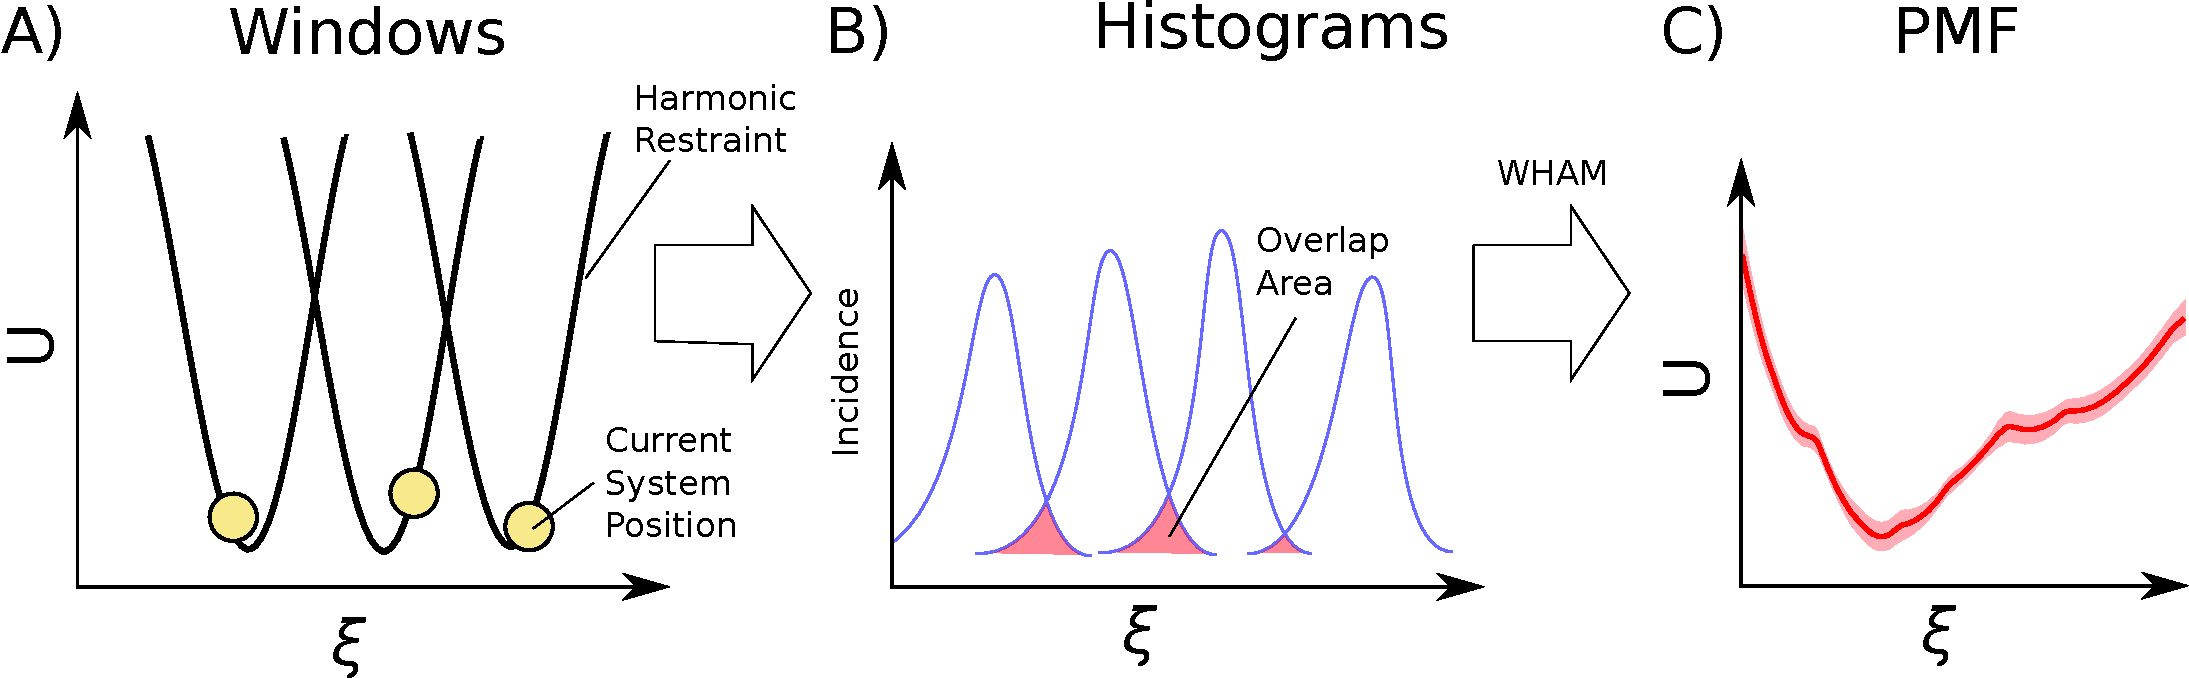
\includegraphics[width=\textwidth]{figures/umbrella_sampling.png.pdf}
	\end{center}
	\captionsetup{singlelinecheck = false, justification=raggedright}
	\caption[Illustration of Umbrella Sampling] {\textbf{Illustration of Umbrella Sampling}}{A) Several simulations are repeated with only one change. A bias  potential is added somewhere along the reaction coordinate $\xi$. B) The value of $\xi$ is recorded in each of the windows and then graphed as histograms. C) The Overlap in neighbouring histograms is integrated via the WHAM method to calculate the Potential of Mean Force. This gives us the energy landscape. Fluctuations in the overlap in the data can be used to estimate the error for the PMF. }
	\label{umbrella_sampling_illustration}
\end{figure}

Umbrella sampling is possibly the most popular method of calculating the free energy of a system along a reaction coordinate. The conceptual philosophy for the method is demonstrated in figure \ref{umbrella_sampling_illustration}. The molecular system is replicated in several ``windows" and a harmonic $U_{biased}$ is added to restrain the collective variable $\xi$ at several different points. The fluctuations of $\xi$ are recorded and the overlap between windows allows us to calculate the potential of mean force (PMF), and thus the energy landscape along the reaction coordinate.  

In more  technical detail, umbrella sampling involves a functional form where $U_{bias}$ separated into $N$ windows. With the bias function in the $n$th window has the form:

\begin{equation}
	U_{b}^n = \frac{k^n_{\xi}}{2}(\xi(\bold{x}) - \xi_0^n)^2
	\label{umbrella_bias}
\end{equation}

Where $\xi_0^n$ is the equilibrium position of the restraint. $k_{\xi}^n$ is the strength of the harmonic restraint in the $n$th window. Typically this is the same in all windows. The more overlap between adjacent windows the more those windows are attracted to each other and the steeper the gradient of the free energy surface (FES) must be pushing those windows together. Conversely, when there is less overlap between adjacent windows it indicates the presence of a barrier in the energy landscape between those windows.

Umbrella sampling is extremely useful for calculating all sorts of experimental quantities and physiologically relevant properties such as folding energies \cite{meshkin2017}, lipid binding \cite{domanski2017}, ion conduction \cite{zhu2012}, and drug binding \cite{subramanian2019}. However, it is particularly sensitive to the choice of initial configuration and collective variable \cite{domanski2017}. The former issue is particular to umbrella sampling because generally short runs are used since so many windows are spawned during the method, the simulations must be at equilibrium \textit{before} the method is attempted, and then sufficient statistics must be collected to average over any conformational changes orthogonal to the collective variable. In these ways, care must be taken when using this method to not introduce systematic error into the calculation \cite{you2019}. A deep knowledge of the molecular system under investigation can help alleviate some of these issues. 

\subsubsection{Weighted Histogram Average Method (WHAM)}
There are a few candidates for calculating a PMF using the statistics calculated in umbrella sampling. The Weighted Histogram Average Method (WHAM) \cite{kumar1992}, Umbrella Integration (UI) \cite{kastner2005} and the Multistate Bennett acceptance ratio (MBAR) \cite{kim2012} are all used. We will briefly outline the mathematical formulation and estimation of errors of the WHAM method as it is more popular \cite{zhu2012}. Our explanation follows \cite{kastner2011} which covers the topic in more detail.

The method begins by dividing the sampled region into a set of $K$ histograms with $K$ being greater than the number of biased windows $N$.  The whole PMF can be estimated (poorly) from the $i$th biased window using 

\begin{equation}
	P_u^i(\xi) = P_b^i(\xi) \exp(\beta U_{b}^i (\xi)) \langle \exp(-\beta U_b^i (\xi))\rangle,
\end{equation}

where the $P(\xi)$  functions represent the probability density function calculated from samples collected at point $\xi$. The samples collected in each histogram then gives us an estimate of the PMF according to equation \ref{unbiased_estimate}. The estimates from each histogram are then combined in a weighted sum using

\begin{equation}
	P_u(\xi) = \sum_i^K p_i(\xi)P_u^i (\xi)
\end{equation}

where the weights, $\sum_{i=0}^N p_j = 1$ are chosen such that the statistical error is minimised across the domain of $\xi$ \cite{chen2011}. This means we solve an optimisation problem for the variance of the unbiased estimates

\begin{equation}
	\frac{\partial\text{Var} (P_u)}{\partial p_i} = 0
\end{equation}

to give the best estimate of the PMF given the samples in each $P_b^i(\xi)$. Essentially we are vertically shifting the estimates obtained in each of the histograms in order to minimise the error across the PMF. 

By convention, we estimate the error in the PMF by splitting up the statistics collected for the distributions of $P^b_i (\xi)$ and constructing PMFs from these independent samples. For example, we might have collected 100 ns of data in each window, but we could construct 5 independent estimates for the PMF using 20 ns blocks of trajectories. The Standard Error of the Mean (SEM) can then be used to estimate the error across the surface \cite{gapsys2020}. By convention, an umbrella sampling calculation is said to have converged when the SEM from these independent samples has fallen below 1 kcal/mol across the PMF. Note that there may be sources of systematic error not captured by this criterion. 

\subsection{Metadynamics}

\begin{figure}
	\begin{center}
		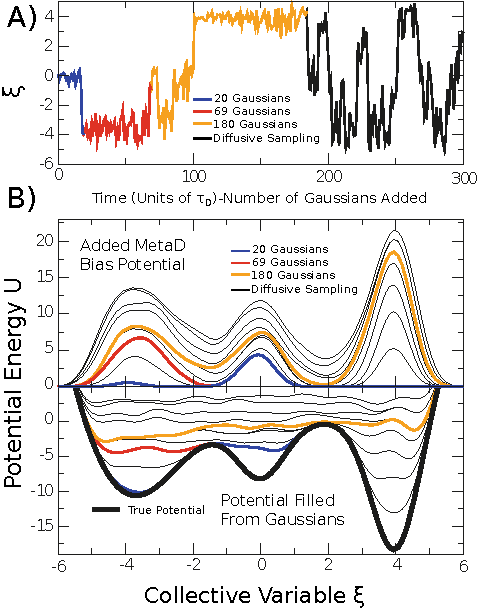
\includegraphics[width=0.7\textwidth]{figures/METAD_demonstration.pdf}
	\end{center}
	\captionsetup{singlelinecheck = false, justification=raggedright}
\caption[Illustration of Metadynamics] {\textbf{Illustration of Metadynamics}}{A) The trajectory of a collective variable $\xi$ in a  metadynamics simulation. The blue region denotes the trajectory up to the time where 20 Gaussians have been deposited. After which the basin at $\xi=0$ has been filled. The red data points denote the time up until 69 Gaussians have been deposited, after which time the second basin at $\xi=-4$ has been adequately sampled. Finally the Orange data indicates that the 3rd basin at $\xi=4$ has been adequately sampled after which which time the system begins to sample $\xi$ diffusively and the simulation has converged. B) The upper panel demonstrates the repulsive potentials that have been added to the simulation in order to drive it to new, unexplored regions. Multiplying the values of this function by $-1$ will be the estimate of the free energy surface\footnote{This is the most simple kind of estimator, used in run of the mill metadynamics but there are more sophisticated estimators for metadynamics variants}. Note how in the lower panel the true potential energy surface is gradually filled by the added Gaussians functions.  Source \cite{bussi2020}}.
	\label{METAD_demonstration}
\end{figure}

Developed in the lab of Michele Parrinello \cite{laio2002}, metadynamics has proven to be a popular method in many applications of computational science, not just in molecular dynamics simulations of biomolecular systems \cite{cheng2017, giberti2015, bussi2020a}. A pedagogical review of the method and its variants written by Pratyush Tiwary can be found in \cite{bussi2020} or by Bussi in \cite{bussi2015}. The method relies on a time dependent form of $U_{bias}$ given by 

\begin{equation}
	U_{bias} (\xi,t) = \sum\limits_{\substack{t' = \tau_D, 2 \tau_D,... \\ t' < t}}  B \ \exp\bigg( - \frac{(\xi(t) - \xi(t') )^2}{2\sigma^2 }\bigg)
\end{equation}

This means that at regular intervals of $\tau_D$ during the simulation we drop virtual, repulsive Gaussian potentials at positions along $\xi$ in order to encourage the simulation to sample regions of $\xi$ it has not visited already. The process is illustrated in figure \ref{METAD_demonstration}. The thermodynamic assumption of this method is that the deposition is done slow enough that the system remains at equilibrium, so a small Gaussian height should be chosen. Usually, the Gaussian widths $\sigma$ are chosen to be the size of the variance in the unbiased measurements of $\xi$. 

The FES estimate at time $t$ from this method is simply the sum of all the Gaussians we have added into the system inverted:  

\begin{equation}
	U_u (\xi,t)  =  \frac{1}{t_c-t} \int_{t_c}^t U_b(\xi,t) dt
\end{equation}

Formally, convergence is reached when the observed probability density is uniform across $\xi$. That is:
\begin{equation}
	P_b (\xi)= \frac{1}{V_\xi } 
	\label{convergence_criterion_metad}
\end{equation}

where $V_\xi$ is the volume of the phase space spanned by $\xi$. However, in practice the function $U_{bias}(\xi)$ is simply inspected at intervals for fluctuations about an average function \cite{sun2016}. 

There are many flavours of metadynamics. The most popular is well-tempered metadynamics which gradually reduces the Gaussian height $B$ as the simulation progresses\cite{barducci2008}. In theory, this guarantees convergence with vanishingly small error. However, this method requires an estimate of how long the simulation will take to converge. There is also infrequent metadynamics which can be used to estimate the diffusion profile along $\xi$ \cite{tiwary2013, tiwary2016, salvalaglio2014, henin2022}.  

A useful feature of the Metadynamics method is that it can be linearly sped up with the number of parallel simulations. This is known as multiple walker metadynamics \cite{raiteri2006}. Since we are simply attempting to sample from the same potential $U_{CHARMM}$ up to a desired time, until the criterion in equation \ref{convergence_criterion_metad} is met, we can speed this process up by running simulations in parallel to sample different regions of $\xi$ and adding Gaussian to the same $U_{bias}$ function.

Conceptually, metadynamics performs the same role as umbrella sampling and should in theory produce the same results in the same system with the same collective variable $\xi$. However, it has some specific contexts where it outperforms umbrella sampling. This method is more suited to an exploration of free energy space where it can intelligently explore regions which are poorly sampled, whereas umbrella sampling requires some foreknowledge of the surface being investigated in order to guess which parts of the landscape require more sampling (in umbrella sampling regions with a high gradient in the FES require a higher density of windows). However, metadynamics can be very difficult to converge. A good indicator of such systematic errors are the presence of unphysically large barriers, indicating that there are orthogonal degrees of freedom not sampled along $\xi$ which might correspond to a minimum energy pathway. These barriers will eventually come down in the infinite sampling limit but many barrier crossings will need to be observed. Excellent discussions of how to solve these systematic errors can be found in articles by Giovanni Bussi \cite{bussi2015, bussi2020a}.

\section{Short Comings of Classical MD}
The short comings of classical molecular dynamics fall into two classes. First is the accuracy of the chemical forcefields outlined in section \ref{forcefields_review}. Second, there is the inability of modern computers to deliver enough samples of the energy landscape to collect sufficient statistics to reach a rigorous conclusion. We are challenged by the physical nature of molecular systems as outlined in section \ref{born-oppenheimer}. The more accurate our forcefields, the more computationally expensive our calculations become, and so the harder it is to deliver a sufficient number of samples. Hence, the solutions to these two problems are diametrically opposed. In the this short section we will explore the current efforts to find solutions to both problems.

\subsection{The Problem with Forcefields}
The approximations inherent in equation \ref{CHARMM_effective_potential_eq} are not without a cost to accuracy. In certain situations, many of which are biologically relevant, it has been shown that polarisation effects not captured by fixed partial charges play an important role in the dynamics of the system. This has been demonstrated in the literature for Gramicidin A, where polarisable forcefields are able to more accurately reproduce the experimental measurements of current \cite{ngo2021}.

The other context where polarisation is important to consider involve divalent ions such as calcium or magnesium. Here, the highly charged environment near a divalent ion will induce changes in the dipole moment of surrounding atoms. This is not possible in the fixed charge formulation in equation \ref{CHARMM_effective_potential_eq}, making investigations of these biologically important chemical species difficult \cite{mamatkulov2013, bergonzo2016}.

However, for most situations, particularly those involving bulk water with a low concentration of solute, classical forcefields are sufficiently accurate to sample conformational motions of biomolecules \cite{hollingsworth2018}. Sadly, it should also be kept in mind that classical MD is not able to simulate any chemistry such as forming and breaking of bonds or a change in the protonation state of an amino acid. Such interactions require considerations of quantum mechanics which are computationally expensive \cite{melo2018}.

There are several efforts to address some of the above issues. Some groups are trying to improve the accuracy of classical forcefields using machine learning and Bayesian inference \cite{nerenberg2018, unke2021}. But there are also attempts to move beyond the functional form of equation \ref{CHARMM_effective_potential_eq} by explicitly including the effects of polarisation. A popular method at the moment is to add a massless drude oscillator as an extra bead to atoms as in the CHARMM drude forcefields, championed by the laboratory of Alexander Mackerell Jr. and others \cite{lin2020}. An alternative solution is to explicitly calculate the dipole and quadrupole moments of each atom at each time step, as is done in the AMOEABA forcefield \cite{shi2013}. These both substantially increase computational cost but have displayed much better agreement with experiments in biological systems, where classical forcefields have been shown to fail \cite{ngo2021, li2017, shi2013}. 

Ultimately, the functional form in equation \ref{CHARMM_effective_potential_eq} used by classical forcefields does not have sufficient degrees of freedom to address all possible chemical contexts. Careful consideration must always be given to whether the forcefield is being used in a faithful way to the situations it was intended to accurately represent. So long as the user is aware of the situations where a given forcefield falls short, classical forcefields can be a powerful tool for the study of molecular systems.

\subsection{The Problem with Sampling}
\label{sampling_problem}

Collecting sufficient statistics about the system of interest is often computationally infeasible in molecular systems. Even though computers have sped up exponentially for the last 50 years we are still orders of magnitude from being able to brute force the time scales of many biological processes, as displayed in table \ref{timescales}.

The slow time step demanded in classical MD due to the fast motions of certain atomic groups such as hydrogen is fundamentally at odds with the time scales of many important biological processes such as drug binding or protein folding which occur on the time scale of milliseconds or seconds.  

Methods are now emerging which can intelligently drive a simulation toward regions unexplored in the collective variable space by unbiased simulations. For some time the field has used steered methods or adaptive sampling methods such as Umbrella Sampling or Metadynamics to drive the simulation toward sections of the energy landscape which are under sampled. These methods universally rely on a choice of collective variable $\xi$ which corresponds to a slow degree of freedom. Such a choice is not usually simple. In the case of ion channels one may rationally choose the placement of the ion along the conduction pathway as the collective variable but the choice is less obvious in the case of more global conformational changes.

The success of simulations at the millisecond timescale by D.E Shaw research suggest that we are in reach of an exciting area in biological research \cite{lindorff-larsen2016, robustelli2022}. Enhanced sampling methods will be able to routinely reach motions that occur on these time scales and as software and hardware improve we will be able to push further, to simulate larger systems. 

The advances we are seeing at the moment which I find exciting are the use of machine learning methods to tease out these degrees of freedom in order to accelerate them with already established enhanced sampling methods. That is, make a more careful choice of the collective variable $\xi$. This could be done with a variety of algorithms such as Principal Component Analysis (PCA) \cite{spiwok2007},\footnote{The use of this collective variable for conformational changes is sometimes called Essential Dynamics.} Time lagged independent component analysis (TICA) \cite{noe2001, schultze2021} from Frank No\"e, a variational approach to conformational dynamics (VACs) from Michelle Parinello's laboratory \cite{brotzakis2019} or Reweighted autoencoded variational Bayes for enhanced sampling (RAVE) \cite{ribeiro2018} from Pratyush Tiwary's laboratory. These algorithms have the potential to build on the above rigorous physics of simulations and revolutionise our understanding of biomolecular systems. As a small example, in chapter \ref{chap:opening} we will discover collective motions using PCA which dilate the CFTR ion channel and study the conduction ions through this dilated structure. 

\section{Conclusion}
It is hoped that the preceding chapter can serve as a roadmap for any physicists interested in beginning to study the exciting field of computational biophysics. The information in each section should serve to help the reader understand the foundations of how simulations are performed. The next steps would be to learn more about the molecular biology and biochemistry of macromolecules so they can better understand the chaotic dance occurring inside cells. For recommended reading on this topic there is Schlick \cite{schlick2010}, Frauenfelder \cite{frauenfelder2010} and Phillips \cite{phillips2012}. There is a lot to learn and the barrier to entry can seem daunting. The reader is encouraged to join mailing lists and other forums where the thriving computational chemistry and computational biophysics communities communicate. Send cold emails asking for help when you are stuck, remember to consult software manuals as well. Below is a list of software to get you started building and running simulations. 

\begin{itemize}
	\item \href{https://www.python.org/about/gettingstarted/}{Python} \cite{van1995python}. A versatile programming language that will help with all parts of a computational workflow.
	\item \href{https://www.ks.uiuc.edu/Research/vmd/}{Visualised Molecular Dynamics} (VMD) \cite{humphrey1996}. Molecular visualisation software with a scripting language, great for building simulation systems, viewing trajectories and rendering figures. 
	\item \href{http://alchemistry.org/wiki/Main_Page}{Alchemistry wiki}. An extensive wiki focussed on pedagogical explanations of alchemical free energy methods. 
	\item \href{https://charmm-gui.org}{CHARMM-GUI} \cite{mallajosyula2015}. A web server which offers a great starting point for constructing MD simulation systems and also offers configuration scripts for all the major MD software packages.
	\item \href{https://www.mdanalysis.org/}{MDANALYSIS} \cite{michaud-agrawal2011, gowers2016}. A python package with a diverse set of tools to analyse molecular dynamics trajectories and structures. 
	\item \href{http://statisticalbiophysicsblog.org/}{Statistical Biophysics Blog} A personal blog by respected computational biophysicist Daniel M. Zuckerman. Here you will find some simple theoretical exercises and some helpful personal advice, not just technical. His book ``Statistical Physics of Biomolecules: An Introduction" is also a very pedagogical introduction to the subject of molecular biophysics.
	\item \href{https://salilab.org/modeller/}{MODELLER} \cite{sali1993, shen2006, webb2016}. A python package which helps build homology models of protein structures or add missing parts to protein models.
	\item \href{https://www.ks.uiuc.edu/Research/namd/}{NAMD} \cite{phillips2005}. A powerful, scalable user friendly MD simulation package.
	\item \href{https://manual.gromacs.org/current/index.html}{GROMACS} \cite{abraham2015}. A less user-friendly MD simulation package than NAMD but offers some different features and (at the time of writing) faster performance.
	\item \href{https://openmm.org/}{OPENMM} \cite{eastman2017}. A flexible MD simulation package that is optimised for usage on GPUs. Is controlled with a python API. A good choice for desktops and workstations.
	\item \href{https://www.plumed.org/}{PLUMED} \cite{tribello2014}. A plugin for existing MD simulation packages which lets the user define their own collective variable $\xi$. Very useful for sophisticated analysis and free energy calculations. 
	\item \href{https://www.rcsb.org/}{Protein Data Bank} (PDB). An open source database of all published biomolecular structures at atomic resolution. 
	\item \href{https://www.uniprot.org/}{Uniprot} \cite{theuniprotconsortium2021}. A database containing a wealth of biochemical data and annotations for proteins, very handy when starting a new project.
	\item \href{https://alphafold.ebi.ac.uk/}{ALPHAFOLD2} \cite{jumper2021}. A highly accurate AI generated database of protein structures. This was considered a watershed moment in the field when it was released.
	\item \href{http://mackerell.umaryland.edu/charmm_ff.shtml}{CHARMM forcefield} \cite{huang2016}. The parameter files for the CHARMM forcefield formatted to be read by popular MD simulation packages.
	\item \href{https://ambermd.org/AmberModels.php}{AMBER forcefield and simulation package} \cite{amber22, ponder2003}. An MD simulation package and toolkit. Here you will also  find instructions for how to extract and use the latest AMBER forcefield in other MD simulation packages.
	\item \href{https://parmed.github.io/ParmEd/html/index.html}{PARMED} \cite{shirts2017}. A python package for converting and manipulating MD file types.
	\item \href{http://www.ccl.net/jobs/} {CCL.net}. A job site where computational chemistry jobs are shared. 
	\item \href{https://www.biophysics.org/} {The Biophysical Society}. The American biophysical society is the largest community of biophysicists. The yearly meetings draw thousands of participants from across the world. At this website you will also find job postings and community news.
\end{itemize}

No individual who has studied a specific discipline has the skills necessary to pick up biomolecular simulation software and begin using it. Physicists lack the understanding of the biology and the chemistry involved in the biological systems, while chemists and biologists may lack an understanding of the deep mathematics that has gone into producing highly accurate simulations of molecular systems. It will take time to get used to an interdisciplinary way of thinking. The reader is also encouraged to seek out collaborators of wet lab disciplines such as cell biologists and protein biochemists to help answer the important problems in biology.

\chapter{Review of Cystic Fibrosis and The Molecular Basis of its Treatment}
\label{chap:cftr}
\chapquote{Because of what's inside me; Because of my genes.}{-Bob Flanagan ``Why?" \cite{dick1997}.}
\newpage
%Authors note:
% We begin with a breif overview of the disease Cystic Fibrosis as it is the main motiation for this project. A horrendous disease for which we will hopefully soon find a cure.

%Clinical outcomes are a chronic illness which affects multiple organ systems and every aspect of a patient's life. 
	%physical therapy, pancreatic sufficiency, ongoing discovery of chronic issues. Much to do. 


% The cause of the disease is CFTR misfunction.
       % CFTR function overview

% CFTR modulators act to restore its function. 
	% patients with rare genotypes cant access modulators.

We aim to elucidate the molecular nature of Cystic Fibrosis (CF)--A disease caused by the misfunction of a protein called the Cystic Fibrosis Transmembrane conductance Regulator (CFTR). In subsequent chapters we will use Molecular Dynamics (MD) to determine how rare mutations cause cause this protein to misfunction. These results are presented with the goal of building a molecular understanding for the treatment of rare CF causing mutations. Given the importance of the CFTR protein system to this work, we will look at its structure and dynamics in some detail in this chapter. In some sections of this chapter I have gone into far more detail than necessary in order to compile details which might serve as a reference text for future endeavours into molecular studies of CFTR. 

To understand the motivation for this level of detail, we will first review some of the medical literature surrounding the disease itself. CF is a multi-system disease with many complications. The management of symptoms can be a significant burden for patients and their families but recent treatments and advancements in translating basic biological research into the clinic has given many hope of a more normal life. 

After this review of clinical outcomes, we will once more work our way upward, as ultimately, CF symptoms are due to the mutation of a single gene. The detailed outline of CFTR structure and function will be our starting point for a physical understanding of CF pathogenesis. This will then be followed by an overview of the mechanism behind the restoration of CFTR by small molecule drugs known as CFTR modulators. 

Here we will also show how to integrate our molecular perspective from simulations with \textit {ex vivo} organoid models grown from a patient's own cells. Results from these organoid models will be presented in subsequent chapters to prove that small molecule drugs appear to be capable of treating a diverse set of molecular phenotypes. In chapter \ref{chap:conclusion} we will combine these results to argue that this personalised approach to medicine leads us to expect that patients with rare missense mutations will likely benefit from existing treatments, but they are currently excluded from accessing due to an outdated understanding of disease pathogenesis. 

The end of this chapter will contain a brief overview of the different experimental techniques which were employed by collaborators of our simulation work to characterise the response of different mutations to different drugs. The language in these sections is kept simple, so the unfamiliar physicist reader can understand some common techniques which they will encounter in the literature surrounding biochemistry and cell biology. The intention here is not replication but comprehension. Hence, an experienced biochemist or a cell biologist would likely find these explanations lacking. For a deeper understanding, the physicist is encouraged to spend lots of time learning from their experimental colleagues, or even perform some of these experiments themselves if possible. 

Another small deviation of this chapter compared to the previous chapters is the chosen structure. In previous chapters we always began with the smallest physically relevant length scale and then worked upward. In chapter \ref{chap:methods} I showed how we can begin from Schr\"odinger's wave equation and work to build simulation techniques which let us understand whole biomolecular systems. This was to give an example of the philosophy outlined in chapter \ref{chap:introduction}, where the physicist designs abstract formalisms and integrates them to model macroscopic physical phenomenon. In this chapter I have made a small but concious deviation from this pattern. Instead of beginning with a discussion of the smallest physically relevant system, the protein which causes disease, we will first discuss some of the clinical realities of living with CF. This deviation from a purely physics inspired structure is made so that we do not lose sight of our goals when studying biophysics.

When one trains to practice medicine they are taught how to conduct themselves ethically, with their patients best interests at heart \cite{hajar2017}. Typically, a physicist has no such training, so they may miss the human aspect of medicine by studying disease impersonally \cite{foucault1994}. 

In subsequent chapters we will work with the theoretical and impersonal tools of molecular physics, to understand the cause and treatment of a disease. We do this in the hope that a physical understanding may improve patients' lives. However, when using such techniques we must always remain aware of how such technologies could be misused in living systems. Consequences of the callous pursuit technological advancement can be seen in the participation of physicists in political and moral discourse in the 20th century. Here, the contributions from physicists were varied and not always for the better \cite{frank1993, gottfried1999, global2009, rhodes1986, aaronson2008, berger2016, vonneumann_britanica}. Should we wish to embark on the enterprise of studying biophysics we have a responsibility to do so ethically. Thankfully, many important questions have been studied by philosophers, and the reader is encouraged to seek texts on bioethics and also ethics in the use of artificial intelligence \cite{buchanan2000, taneri2011, genome_editting_guildelines_2017, muller2021, bostrom2014, roose2022}. These considerations are likely to become increasingly important---as biophysics advances, so too does its capacity for misuse \cite{mallapaty2022, urbina2022}. 

%The reader is asked to keep this responsibility in mind in the subsequent chapters where we have worked with basic, impersonal theoretical tools in molecular physics. These techniques were understand the cause and treatment of Cystic Fibrosis. This work was performed in the hope  do this in the hope that an increased understanding may may improve patients' lives. We must be aware of the moral pitfalls that a single minded pursuit of a physical understanding of living systems presents. We must be aware moral challenges that this represents. In the 20th century, physicists often participated in political and moral discourse, and not always for the better \cite{frank1993, gottfried1999, global2009, rhodes1986, aaronson2008, berger2016, vonneumann_britanica}. Should we wish to embark on the enterprise of studying biophysics we have a responsibility to also study how to do it ethically. Thankfully, many important questions have been studied by philosophers, so the reader is encouraged to seek texts on bioethics and also ethics in the use of artificial intelligence \cite{buchanan2000, taneri2011, genome_editting_guildelines_2017, muller2021, bostrom2014}. These considerations are likely to become increasingly important---as biophysics advances, so too does its capacity for misuse \cite{mallapaty2022, urbina2022}. 


%On this somewhat somber note, we will now take a brief look at what it is like to live with Cystic Fibrosis.

%We will then analyse the root cause, mutations to the Cystic Fibrosis transmembrane Conductance Regulator (CFTR). In chapter \ref{chap:conclusion} we will use much of the knowledge gained in this chapter to think about where we can direct future studies to help treat the root cause of Cystic Fibrosis. 

\section{Clinical Realities of Living with Cystic Fibrosis}
\label{clinical_realities_CF}
Cystic Fibrosis (CF) is the most common fatal genetic condition in Caucasian populations. Over 162 000 people are estimated to be afflicted globally, with a significant proportion living undiagnosed \cite{hammoudeh2021,guo2022}. Even with decades of research there is no known cure for CF and patients currently have a life expectancy below 50 \cite{mcbennett2022}. Management of disease symptoms also bears significant financial and emotional costs to patients and their families \cite{vangool2013, page2022}. From a cellular perspective, the symptoms of the disease are due to the inability of certain cells to regulate their salt content, causing an osmotic imbalance (Figure \ref{CF_summary}) \cite{reddy2013}. 

\begin{figure}
	\label{CF_summary}
	\begin{center}
	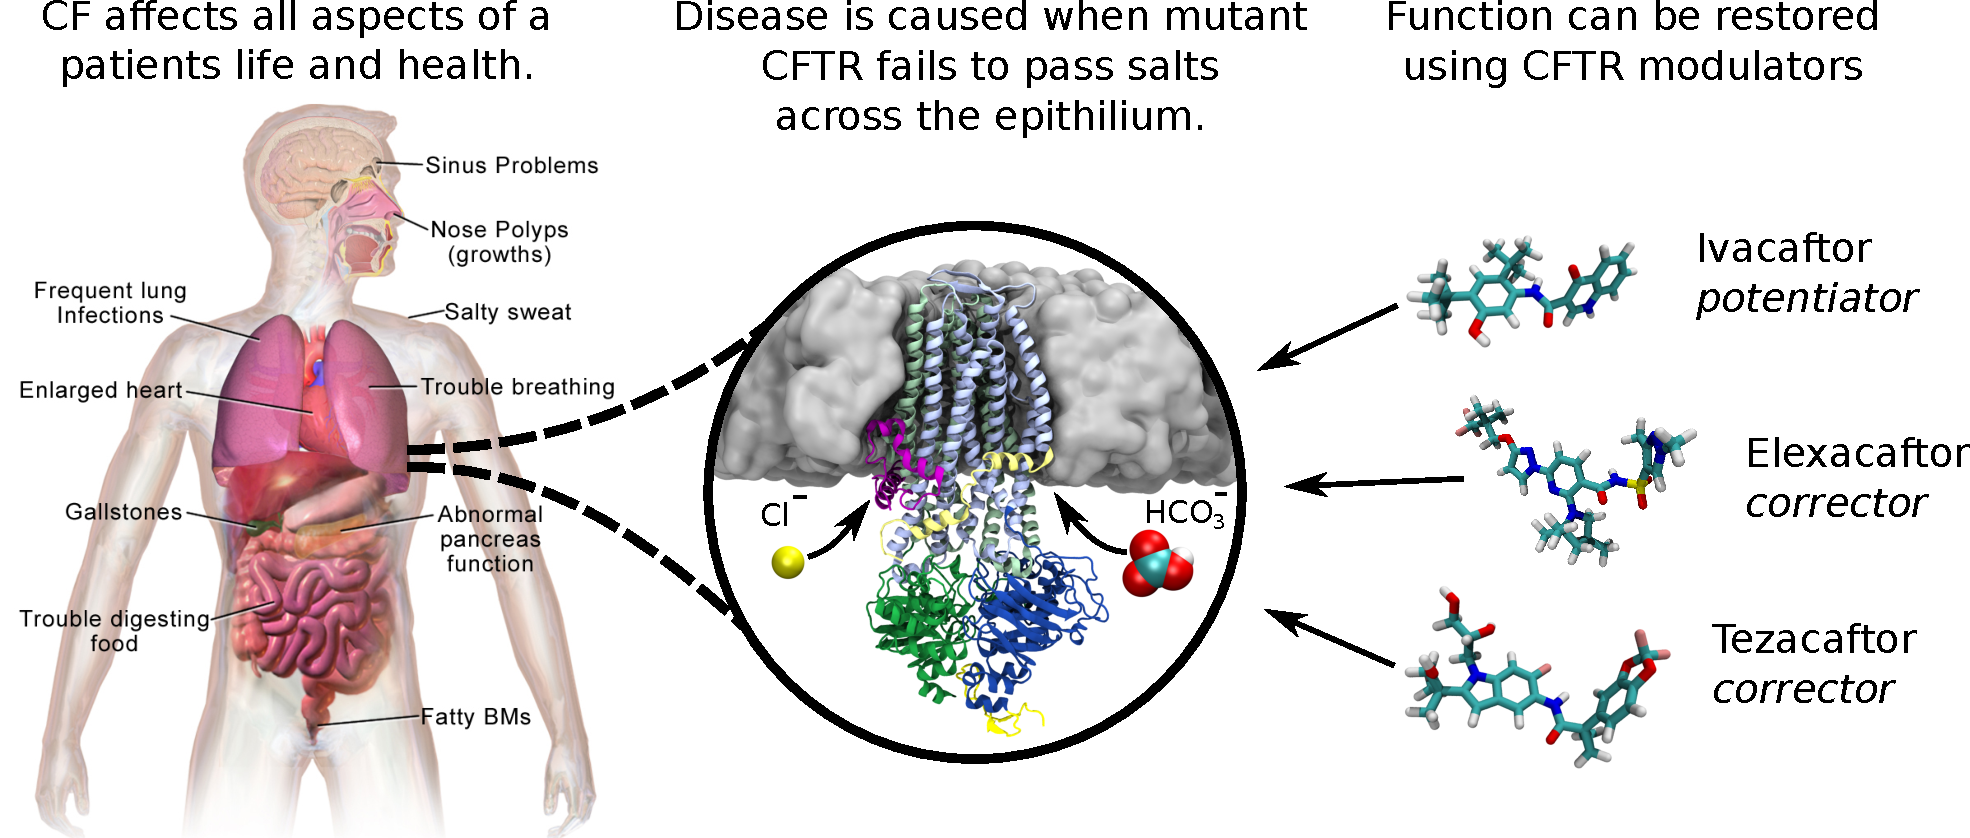
\includegraphics[width=1\textwidth]{figures/cf_summary_fig.pdf}
	\end{center}
	\captionsetup{singlelinecheck = false, justification=raggedright}
	\caption[Cystic Fibrosis is a Debilitating Disease Whose Cause is Genetic] {\textbf{Cystic Fibrosis is a Debilitating Disease Whose Cause is Genetic}}{Cystic Fibrosis causes misfunction in several major organ systems, affecting all aspects of a patients' life and health. The cause of the disease is genetic, when two defective copies of an anion channel gene, CFTR, are inherited from each parent, epithelial cells cannot pass chloride or bicarbonate ions, leading to a pathogenic buildup of salts inside epithelial cells. In recent decades, small molecule drugs have been discovered which act directly on CFTR to restore its function. This thesis seeks to understand what kind of defects these drugs are capable of rescuing. We find that they are likely to rescue a wide range of defects.} 
\end{figure}

All organs of the body are lined by cells called epithelia. They protect organs from trauma and infection. The most acute symptoms of CF are due to the dehydration of this lining. When dehydrated, fine, motile structures on the epithelium called cilia collapse, rendering them unable to ``beat" in order to clear mucus and pathogens \cite{boucher2007, szczesniak2017}. Simultaneously, this mucus which naturally lines the epithelium, thickens as moisture is leached away from it by osmotic pressure.

This thickened mucus has pathogenic effects in several organ systems. The most acute symptoms occur in the lungs where bacterial colonies grow and form a biofilm. This damages the organ and remains one of the most troublesome chronic complications for CF patients \cite{chiappini2014, krouse2001}. Frequent infections mean that patients rely on antibiotics and avoid other people with CF in case they expose each other to new or drug resistant pathogens \cite{conway2008, baldoni2019}. 

In addition to these bacterial colonies, the buildup of mucus inhibits the normal function of the lungs, limiting their ability to absorb oxygen. Patients often undergo hours of physical therapy each day to help them clear this mucus from their lungs \cite{chest_pt_CFF,thefreylife2015}. Inhalation of a saline solutions may also help relieve symptoms, as this draws moisture out of the epithelial cells by counteracting the pathogenic osmotic pressure gradient \cite{wark2018}. As Figure \ref{CF_life_expectancy} indicates, much of the increased life expectancy for people with CF has been due to the improved management of this mucus and the populations of bacterium infecting it \cite{mcbennett2022}. 

In CF care, maintaining lung function remains the primary concern. The organ gradually fails over the course of the patients life, meaning respiratory failure is usually the cause of death \cite{kumar2018}. The adoption of lung transplants has lead to a significant increase to the life expectancy of CF patients but patients may be excluded from receiving a transplant for a variety of reasons \cite{blatter2015, weill2018}. Double lung transplants remain the only option for CF patients as the donor lung would become infected with bacteria from the CF afflicted lung left in their body \cite{mcbennett2022}. 

To track disease progression, the most commonly used biomarker is FEV1\%. This stands for Forced Expiratory Volume in 1 second. It is a measure of the volume of air a patient is able to forcibly expel in one second, compared to their total lung capacity \cite{szczesniak2017}. Once a patient's FEV1\% falls below a certain level (30\%-50\%) they will usually begin to consider a lung transplant if they are eligible \cite{adler2009}.

CF also causes acute and chronic issues in the digestive system. Due to the buildup of mucus, the large intestines struggle to absorb nutrients and the pancreas cannot secrete digestive enzymes. These complications can lead to CF related diabetes which afflicts roughly half of adults with CF \cite{Kayani2018}. To manage and avoid this complication, patients are administered digestive enzymes and consume a high fat diet \cite{sullivan2017}. A patient whose pancreas does not produce sufficient enzymes to digest nutrients is referred to as ``pancreatic insufficient" (PI). This is an important determinant in the severity of disease and a patients' quality of life \cite{halloran2011,singh2017}. 

\begin{center}
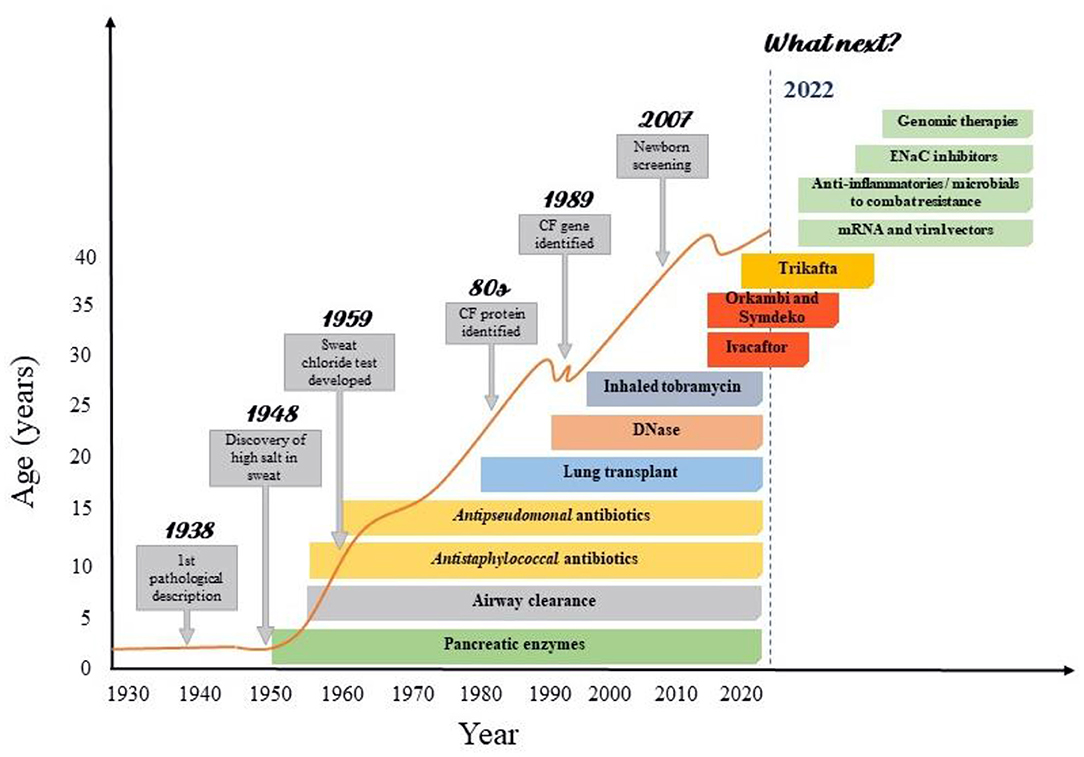
\includegraphics[width=0.7\textwidth]{figures/CF_life_expectancy.png}
\end{center}
%\captionsetup{singlelinecheck = false, justification=raggedright}
\begingroup
\captionof{figure}[CF Clinical Progress] {\textbf{CF Clinical Progress}}{The orange line depicts the life expectancy of CF patients in relation to the development of different treatment. Life expectancy correlates highly with translational research. As CF becomes a chronic condition patients will likely undergo a combination of more and more advanced therapies. Source \cite{garcia2022}} 
\label{CF_life_expectancy}
\endgroup

Figure \ref{CF_life_expectancy} displays something quite interesting. As patients live longer, CF care must address more disease complications. For example, once pancreatic enzymes were routinely administered, patients began to live beyond two years old \cite{roberts1957, levy2011}, which lead to an to an increasing need to study and manage the role of bacterial infections in the CF lung \cite{burns2001}. With the advent of modulators and refinements to existing therapies, the face of the disease will change. Now that patients are living past 40 we must confront new complications such as bone disorders and infertility \cite{stalvey2013, popli2007}. This means that there still a need to study the cellular and molecular nature of CF, both its root cause and the cause of complications. 


\section{The Misfunction of CFTR Causes Cystic Fibrosis}

We will now begin our journey upward. As we mentioned in the introduction, we will be collecting molecular details about the ion channel at the core of CF pathogenesis to understand the disease and its treatment. Hence, the next sections will outline in considerable detail, the structure, function and misfunction of the CFTR anion channel. 

CFTR is unique. It is a type of protein known as an ABC transporter, designated ABCC7. The ABC super family of proteins bind ATP and use the energy from hydrolysis (breaking) ATP to pump different substrates across the cell membrane, against a concentration gradient. But CFTR does not act as a transporter like the other members of its family. Rather, it can be thought of as a ``leaky pump" since it moves through through a gating cycle but is unable to move its substrate against against a concentration gradient \cite{gadsby2006,linsdell2018}. It is possible that the evolutionary misappropriation of this protein from a transporter into an ion channel is the reason for the large number of mutations which cause it to misfunction \cite{infield2021}. 

%Hence, as CFTR is an \textit {ion channel}, meaning it allows the passive diffusion of chloride and bicarbonate, but it can also pass larger anions such as glutathione (figure \ref{}) \cite{gadsby2006, tang2009,linsdell1998}. 

\subsection{CFTR structure and function}

\begin{figure}
	\begin{center}
	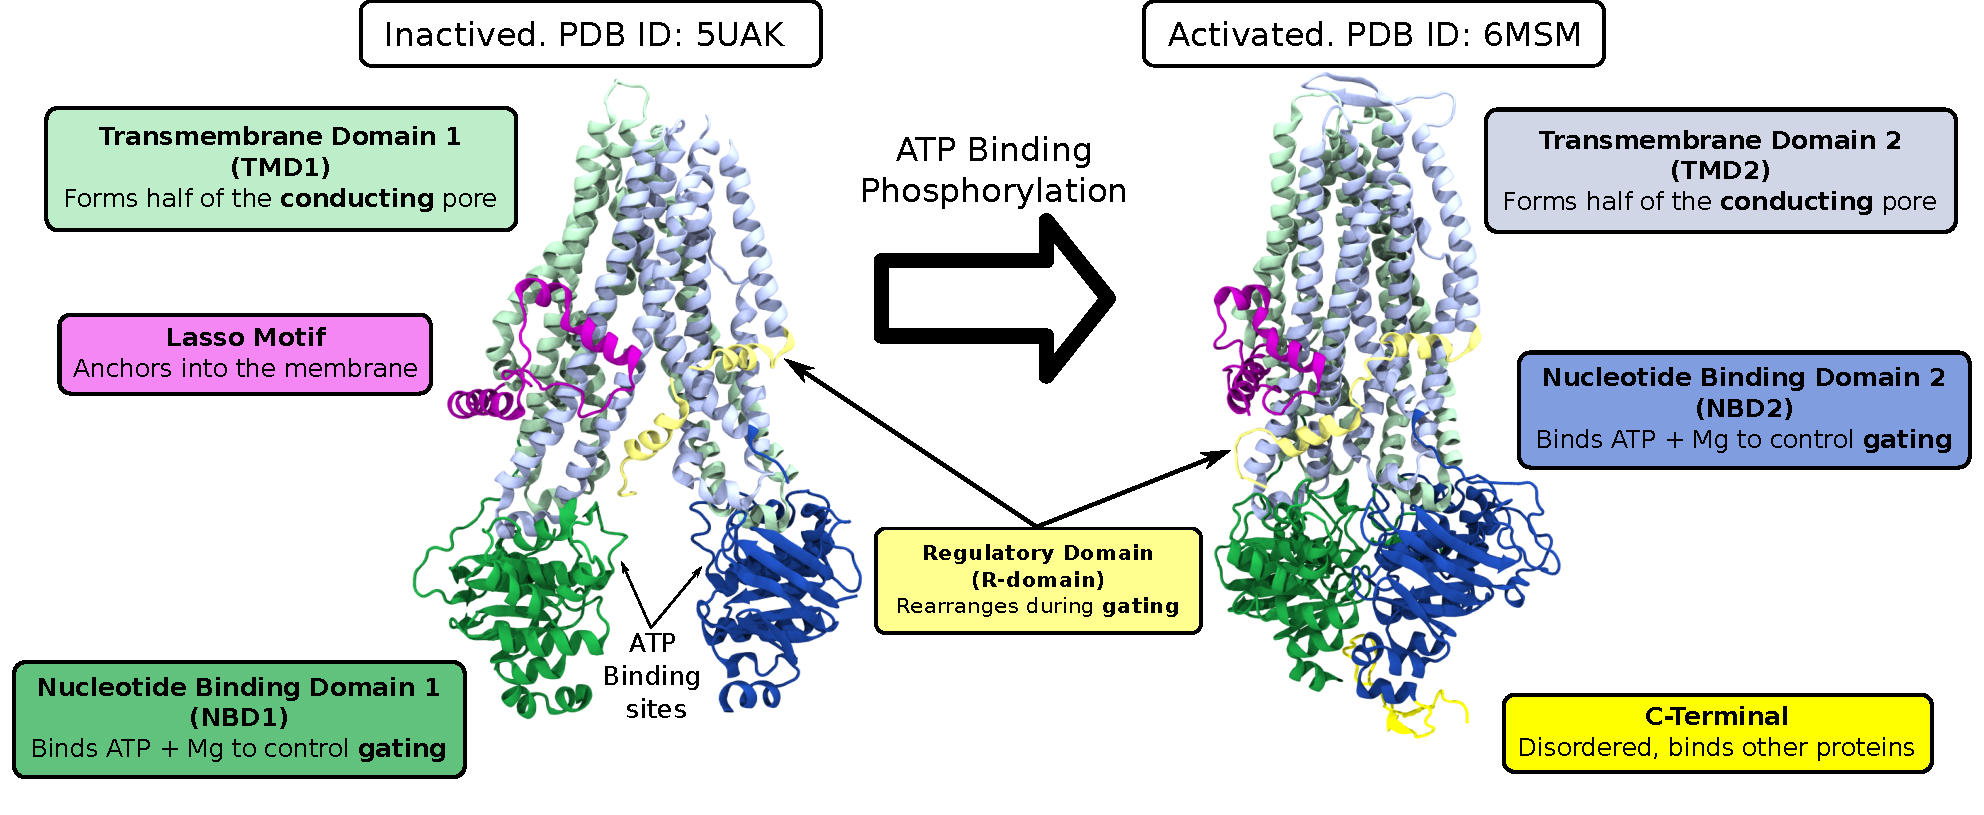
\includegraphics[width=\textwidth]{figures/CFTR_structure.pdf}
	\end{center}
	\label{CFTR_structure_domains}
	\captionsetup{singlelinecheck = false, justification=raggedright}
	\caption[CFTR Structure] {\textbf{CFTR Structure}}{There are currently two conformations of the human CFTR protein which have been imaged at atomic resolution. These cryo-EM structures have captured hCFTR in an inactivated and an activated conformation. The inactivated state (PDB ID: 5UAK) is neither phosphorylated nor bound to ATP. Observe how the NBDs are far apart and the TMDs are not parallel, forcing a constriction near the top of the protein which does not allow the passage of ions. By contrast, the activated structure is bound to two ATP molecules (PDB ID:6MSM), dimerizing the NBDs and bringing the TMDs into a parallel configuration where they are able to form a pore. Despite having the biochemical characteristics which we would expect from the conducting conformation of this ion channel, the available structure of the activated hCFTR protein exhibits a constriction at the extracellular end of the channel which does not allow chloride ions to pass through. In chapter \ref{chap:opening} we will demonstrate enhanced sampling techniques to study a fully conducting CFTR conformation, based on this activated structural snapshot. All simulations presented in this work were based on the ATP-bound phosphorylated human CFTR structure (PDB ID: 6MSM) \cite{zhang2018}.} 

\end{figure}

As an ATP stimulated ion channel, CFTR sits in an inverted ``V" configuration in the cell membrane until it is activated by chemical messengers like ATP and PKA \cite{zhang2018, gadsby2006, mihalyi2020}. When it is phosphorylated, the protein transitions to form a continuous pore. This is the conformational change visualised in Figure \ref{CFTR_structure_domains}.

Chemically speaking, the protein is composed of a single chain of 1480 amino acids.  This chain folds into a pseudo-symmetric structure, organising CFTR into 7 domains. In the order of their primary structure they are: 

\begin{enumerate}
	\item The Lasso motif (AA 1-68), Which anchors into the membrane and serves as an interaction hub with protein partners such as syntaxin and filamin which are important in cellular trafficking \cite{cormet-boyaka2002, naren1998, thelin2007}. 
	\item Transmembrane Domain 1 (TMD1, AA 69-376). This domain forms half of the chloride conducting pore and importantly, TM1 and TM6 in this domain form the extracellular end of the pore for anion permeation \cite{linsdell2006, linsdell2022}. Most positive amino acids which directly interact with anions are located in this domain, even in the inner vestibule \cite{linsdell2018}. We will look at many of these amino acids in detail in chapters \ref{chap:R352Q} and \ref{chap:opening} \cite{wong2022a}. There is a pocket in this domain which also serves as a binding site for both corrector class drugs and protein partners such as WNK1, which stimulates the conductance of bicarbonate \cite{kim2019}. 
	\item Nucleotide Binding Domain 1 (NBD1, AA 377-629). One of the ATP binding sites. This domain has a dense concentration of disease causing mutations, including the most common mutation $\Delta$F508 \cite{cftr2}. This domain contains a Walker A motif but lacks a Walker B motif. This causes one of the ATP binding sites to be degenerate meaning it cannot hydrolyze ATP. 
	\item Regulatory Domain (R-domain, AA 630-855). A disordered domain containing more than 11 phosphorylation sites \cite{mihalyi2020}. In the inactivated conformation of CFTR, a helical segment of this domain wedges between the TMDs. Binding to PKA encourages this helix to unwedge from between the TMDs, while phosphorylation causes the disordered domain to remain in solution. This process has important consequences for the function of the channel \cite{ostedgaard2000, mihalyi2020, bozoky2013, baker2007}. In the open state, the wedge relocates to a location just below the lasso motif \cite{zhang2018}. The identity of the wedge fragment will be analysed in detail in chapter \ref{chap:I37R} \cite{wong2022}. 
	\item Transmembrane Domain 2 (TMD2, AA 856-1168). This domain forms the other half of the chloride conducting pore. There is some controversy over the structure and function of TM8 in CFTR \cite{hegedus2022, liu2019}. This helix plays a critical role in regulating channel gating and anion selectivity \cite{negoda2019}.
	\item Nucleotide Binding Domain 2 (NBD2, AA 1169 - 1450). One of the ATP binding sites. This domain is home to a conserved Q-loop, which regulates the binding of ATP in ABC transporters \cite{ivey2020, zolnerciks2014, dong2015}. NBD2 contains both a Walker A and a Walker B motif, allowing ATP binding and hydrolysis at what is known as the consensus binding site. 
	\item C-terminus (AA 1451 - 1480). This domain is natively disordered but it serves as an interaction hub in WT-CFTR, anchoring CFTR to other proteins in the cell through its PDZ binding domain \cite{moyer1999, cushing2008}. 

\end{enumerate}


%CFTR is distinguished by a regulatory region known as the R-domain (residues 645-845) which links NBD1 to TMD2. This region acts to lock the channel in the closed state by wedging itself between the TMDs and dislodging when any one of 3 sites are phosphorylated \cite{mihalyi2020}. In experimentally determined structures of human CFTR the secondary structure of a section of the R-domain but not at high enough resolution to determine the identity of individual side chains \cite{zhang2018, zhang2016}. Further secondary structure information can be found through experiments with NMR \cite{Baker2007}.

\subsection {Previous MD Studies of CFTR}
Because the first structure of human CFTR was only published in 2017 \cite{liu2017}, previous computational studies of CFTR have had to rely on homology models. More recently these were based on the phosphorylated zebra fish protein ( PDB ID:5W81) \cite{zhang2017a} or for a longer time, a distantly related bacterial ABC transporter SAV1866 ( PDB ID:2HYD) \cite{dawson2006, Hoffmann2018}. These studies have yielded interesting results but it is often hard to translate their findings to the human protein. Even in the zebra fish CFTR protein, the similarity to the human amino acid sequence is only 55\%. This raises some concerns. As we will see, CFTR is a highly sensitive protein, its function is poorly conserved under mutations. Note for example how note is how the action of certain drugs is not conserved in zCFTR \cite{laselva2019}. Additionally, the short time scales (rarely reaching 500ns) of the simulations in these studies opens the possibility that the homology model of the protein remained trapped in local minima, raising questions as to the reliability of their findings.  

Despite their short comings the publications which employed these homology models to investigate the basic function of the CFTR protein have a few notable findings which we will discuss briefly. 

Perhaps the most interesting molecular study from this era used path-CV metadynamics to propose open state of the channel by steering a zebra fish based homology model toward fully outward facing conformation of SAV1866 \cite{Hoffmann2018}. The resulting model has several characteristics expected of the open channel, such as the critical R117-E1124 and R352-D993 salt bridges. However, it fails to create a narrow selectivity filter, which we would expect given results from \textit{in vitro} biophysical experiments \cite{linsdell2016, linsdell2017, linsdell2021, li2018b, linsdell2020, negoda2019}. Additionally, the free energy landscape in this study does not actually display a free energy well at the coordinates which the authors state corresponds to the open state, nor did they validate their open structure with long unbiased simulations (runs were truncated after 50ns). This raises some questions as to whether their proposed open conformation was indeed stable in their model system. However, it was the innovative use of metadynamics in this study which served as the inspiration for the extensive free energy calculations in chapter \ref{chap:opening}. Hence, it was this ambitious study which allowed us to discover a fully open conformation for the human channel. 

A more recent study again employed metadynamics with the zebrafish structure, to study the permeation of chloride through the two extracellular portals in zCFTR \cite{farkas2020}. Unfortunately, this confirmed a difference between the zebrafish and the human structures. Experimental studies indicate that only one extracellular portal is present in the human structure \cite{linsdell2018}. 

Another study, still under review at the time of writing, attempted to resolve the chloride permeation pathway in the same human, phosphorylated CFTR structure which we have investigated in this thesis \cite{zeng2021}. Here, Zhi Zheng, working under Reggis Pomm\'es used unbiased MD coupled with an induced 500mV membrane potential. This strong electric field was used to encourage chloride ions to move through the channel. This study was successful in observing 17 conduction events in 10$\mu$s of unbiased sampling. Although excellent progress, this is an order of magnitude below the number of conduction events we would expect from this level of sampling--given that the conductivity of the open conformation in WT-CFTR is 0.7pS \cite{kogan2003,linsdell1998}. These implications will be discussed in chapter \ref{chap:opening}.

There are some additional MD and docking studies which have either dealt with the effects of mutations or the action of CFTR modulators and they will be discussed in the relevant sections of this chapter (section \ref{} \ref{} respectively )\cite{billet2020, sabusap2021}.

In terms of the basic investigation into the function of CFTR, the final study we will discuss simulated of both human and zebra fish structures were used to study the conformation of TM8 in TMD2 \cite{corradi2018}. As we will discuss in detail in chapter, \ref{chap:conclusion} all CFTR structures solved by the Chen lab exhibit an unusual fold in TM8 \cite{fiedorczuk2021, liu2017, liu2019, zhang2016, zhang2018a, zhang2017a}. The helix unwinds in the middle of the membrane, a configuration that was initially thought to be energetically unfavourable. At the time of writing, there are some unresolved questions as to how this conformation is consistent with low resolution structures of chicken CFTR solved by another laboratory \cite{fay2018}. However, most recent studies have supported the TM8 model found by the Chen lab \cite{corradi2018, negoda2019}. 

In summary, with some exceptions, it is difficult to draw from the previous \textit{in silico} literature of CFTR because studies have lacked an appropriate structure as a starting point. Previous CFTR homology models have largely failed to capture critical molecular details of the full human CFTR protein. Hence these studies mostly served as a proof of concept and inspiration for further work, rather than giving results which can be directly inferred for the hCFTR protein. 

% , it lacks a salt bridge between R104-E116. In experiments, these residues could be replaced by cysteines and the channel would still function. However, when reducing agents were added to the system the channel lost its ability to open fully. This indicates that in the oxidised environment the C104-C116 cysteines formed a disulfide bridge but its breaking upon exposure to reducing agents caused a loss of function in the channel. This indicates that in the WT channel R104-E116 form a stable salt bridge. 

%This salt bridge is clearly visible in the recent cryo-EM structure of ATP-bound human CFTR \cite{zhang2018}.

\subsection{Catalytic and Conformational Changes During the Gating Cycle}

	\begin{center}
	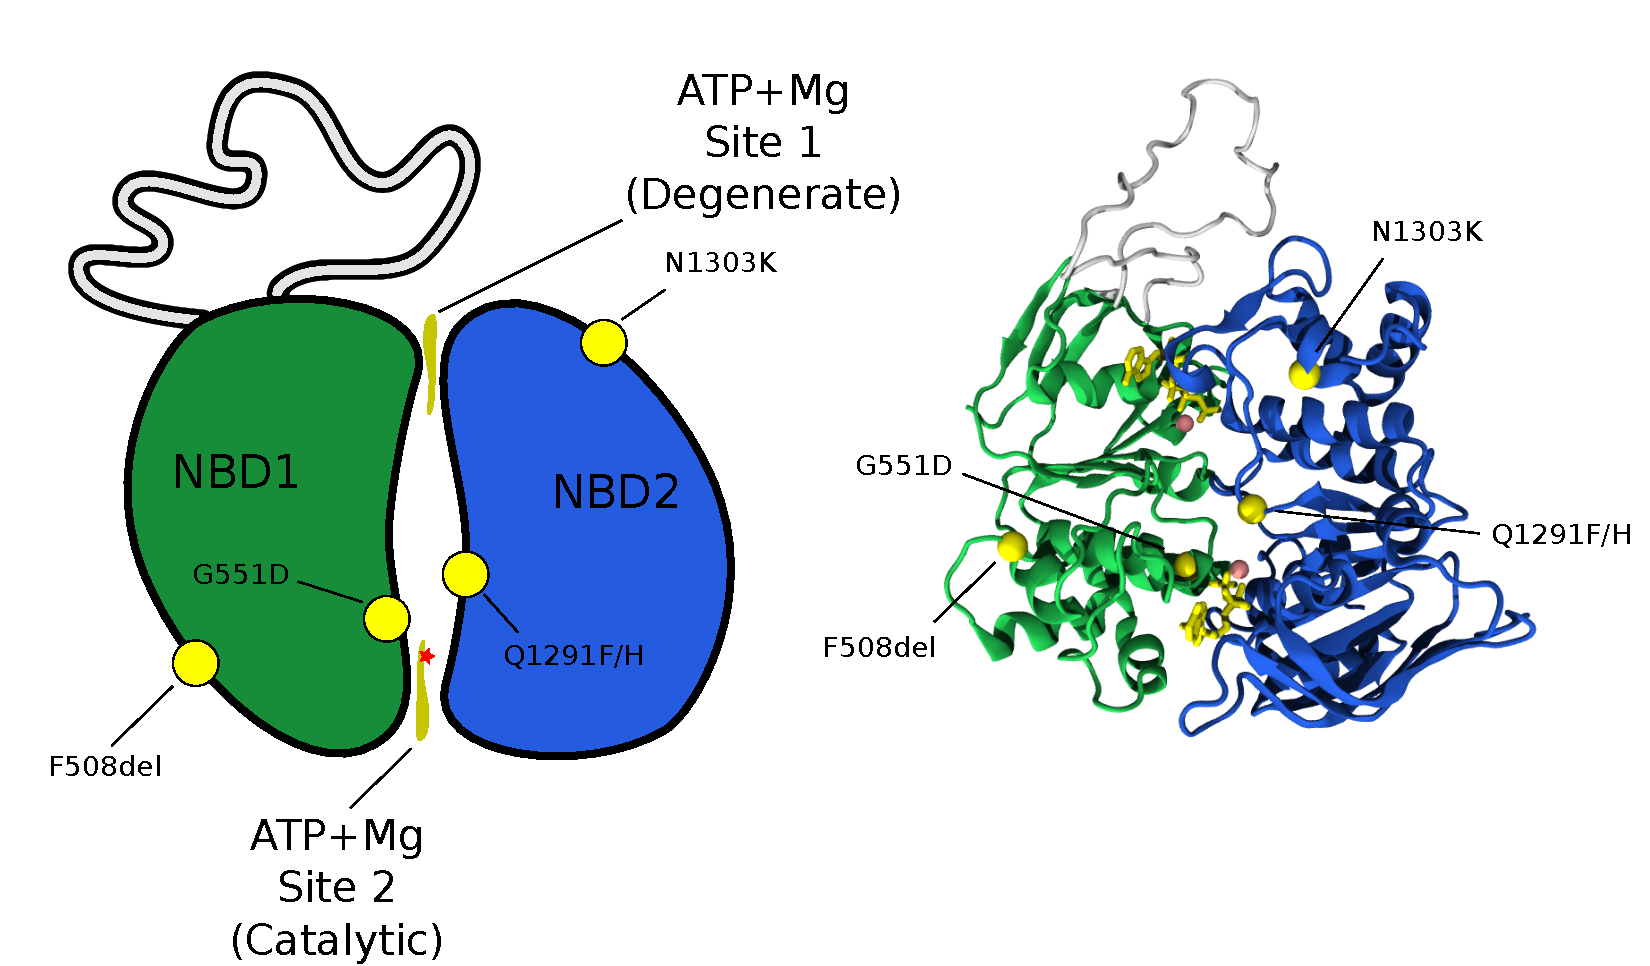
\includegraphics[width=0.8\textwidth]{figures/ATP_head_to_tail_figure.pdf}
	\end{center}
	\begingroup
	%\captionsetup{singlelinecheck = false, justification=raggedright}
	\captionof{figure}[NBD Organisation] {\textbf{NBD Organization}}{A) The NBDs are critical to the gating cycle of CFTR. They rest below the TMDs where they bind and hydrolyse ATP in order to regulate the gating cycle. B) Each NBD contacts both ATP molecules. This configuration is known as a head to tail dimer and is common amongst ABC transformers. One of the unique aspects of CFTR is the fact that only one of the ATP binding sites is capable of breaking down its ATP molecule through hydrolysis \cite{stratford2007}. When ATP is hydrolysed at site 2, the channel is allowed to close \cite{infield2021}. The regulatory insertion another unique feature of CFTR and has been shown to increase NBD1 stability when deleted. The  C) Molecular details of how the NBDs bind ATP at the two binding sites. Here we have highlighted several molecular details. The Walker A motifs are on both NBDs and are responsible for stabilising ATP in a conformation which allows hydrolysis to produce ADP and a phosphate group \cite{deltoro2016}. The Walker B motif on NBD2 is directly responsible for mediating hydrolysis, by allowing the movement of the magnesium cofactor \cite{urbatsch2000, rai2006}. Mutation of E1371 in Walker B is sometimes engineered to kill catalytic activity and lock the channel in an open state \cite{stratford2007, zhang2018}. Note the placement of both G551D, a gating mutation and Q1291H/F near site 2. The most common disease causing mutation $\Delta$F508 is located on a helix of NBD1 which buries itself into a hydrophobic pocket. N1303K is located at a roughly symmetric position on NBD2. } 

\label{NBD_structure}
\endgroup

The conformational transition from inactive to active differs significantly in CFTR compared to other ABC transporters. A transporter is characterised by acting as a gate to substrate, There is never a continuous path to allow the substrate to diffuse passed the protein. Since it is a channel, CFTR gives rise to a continuous pore \cite{linsdell2018}. 

CFTR's gating cycle is dominated by the action of the NBDs and the R-domain. The NBDs are largely similar are largely similar to other transporters in the ABCC subfamily so we will discuss them first. 

NBD1 and 2 each have two binding sites for an ATP$+$MG$^{2+}$ complex. This facilitates their dimerization in what is known a ``head to tail" configuration where both NBDs make contact with both bound ATP molecules \cite{gout2012}  (Figure \ref{NBD_structure}). Usually, in an ABC transporter the NBDs would contain contain a ``Walker A motif" to help them bind ATP \textit {and} a ''Walker B" motif to catalyse the hydrolysis. A unique aspect of CFTR is that NBD1 is missing its Walker B motif, meaning one of the ATP binding sites is incapable of hydrolysing ATP. This ATP binding site is sometimes referred as ``site 1", ''the degenerate site" or ''the non-consensus site" and it plays an important role in stabilising the open state of the channel \cite{yeh2022, csanady2019a}.

The other ATP binding site is referred to as ``site 2", ''the catalytic site" or the ''consensus site." The hydrolysis of ATP at this site triggers the closure of the channel. Sometimes, for the purposes of experiments, the catalytic activity of site 2 is intentionally halted through an engineered mutation. For example, E1371Q-CFTR is studied in structural determination experiments as it exhibits a much longer lived open state than the WT channel. This allows more snapshots to be taken of the open structure during cryo-EM experiments \cite{ramjeesingh1999, gout2012, muallem2009, hwang2013}. Indeed, the protein structure which was the source for our work carried this mutation and it had to be corrected to match the WT amino acid sequence before simulation \cite{zhang2018}. 

The above outlines the generally agreed upon chemistry about the action of the NBDs and gating. Beyond this there are some details about the gating cycle which are still up for debate. There are two competing models which give different predictions for how tightly coupled the dimerization of the NBDs is to the opening of the channel \cite{yeh2022}. The first proposed model is called the ``strict coupling model", which suggests that the NBDs and the TMDs rotate as rigid bodies, to move between the active and inactive states. This model would indicate that ATP binding and NBD dimerization is tightly coupled to the opening of the channel \cite{jih2012}. 

The second model is called the ``energetic coupling" model. This predicts that there are both closed and open states which are accessible while the NBDs are dimerized in the post hydrolytic state, as well as closed and open states while the NBDs are \textit{not} dimerized \cite{jih2012}. This means we would expect that we would expect the binding of ATP to be loosely coupled to the opening of the channel. It would seem that, although more complicated, the second model is both more consistent with recent findings in the literature and would also explain some of the other controversies surrounding the structure and function of CFTR, such as the strange, flexible conformation of TM8 \cite{fay2018}. These considerations are not critical for the work in this thesis but considering them in the future them may aid in targeted drug discovery efforts for CFTR, particularly for potentiator class drugs.

%allows nucleophilic attack by surrounding water on the phosphate tail of the ATP bound to site 2 B \cite{stratford2007}. Since the hydrolysis of ATP causes the channel to gate back to the closed conformation, mutations like E1371Q can be employed studied in contexts where one wishes to lock the channel in an open state such as structural determination 

Apart from the NBDs, the most important domain for the gating of CFTR is the R-domain. This disordered domain is unique to CFTR. In the inactive state the R-domain wedges between the TMDs, forming a plug and not allowing them to rotate to form a pore. Intermittently, Protein Kinase A (PKA) will bind to one of many segments on the R-domain coaxing the coils of peptide out into solution \cite{mihalyi2020}. PKA may then phosphorylate specific sites on the domain, causing it to remain in an unplugged configuration. It is currently unknown exactly how many phosphorylation sites there are in the R-domain, but more than 11 have been investigated \cite{mihalyi2020}. 

When the R-domain is phosphorylated it no longer rests between the TMDs. Rather, the amino acids which form the plug relocations to a site below the lasso motif. This was one of the main findings from chapter \ref{chap:I37R}. Further, in chapters \ref{chap:I37R} and \ref{chap:S945L} we demonstrate how the destabilisation of this binding site results in a gating defect.  

%\footnote{Note to physicists, phosphorylation is a process where a phosphate group is added to the side chain of an amino acid. Usually serine, tyrosine or threonine. This phosphate group a charge of -2, wheres these amino acids are normally neutral. This is a key regulator of protein activity as it places a very large charge at a normally neutral site in the protein.}


\subsection {Anion Selectivity}

\begin{figure}
	\begin{center}
	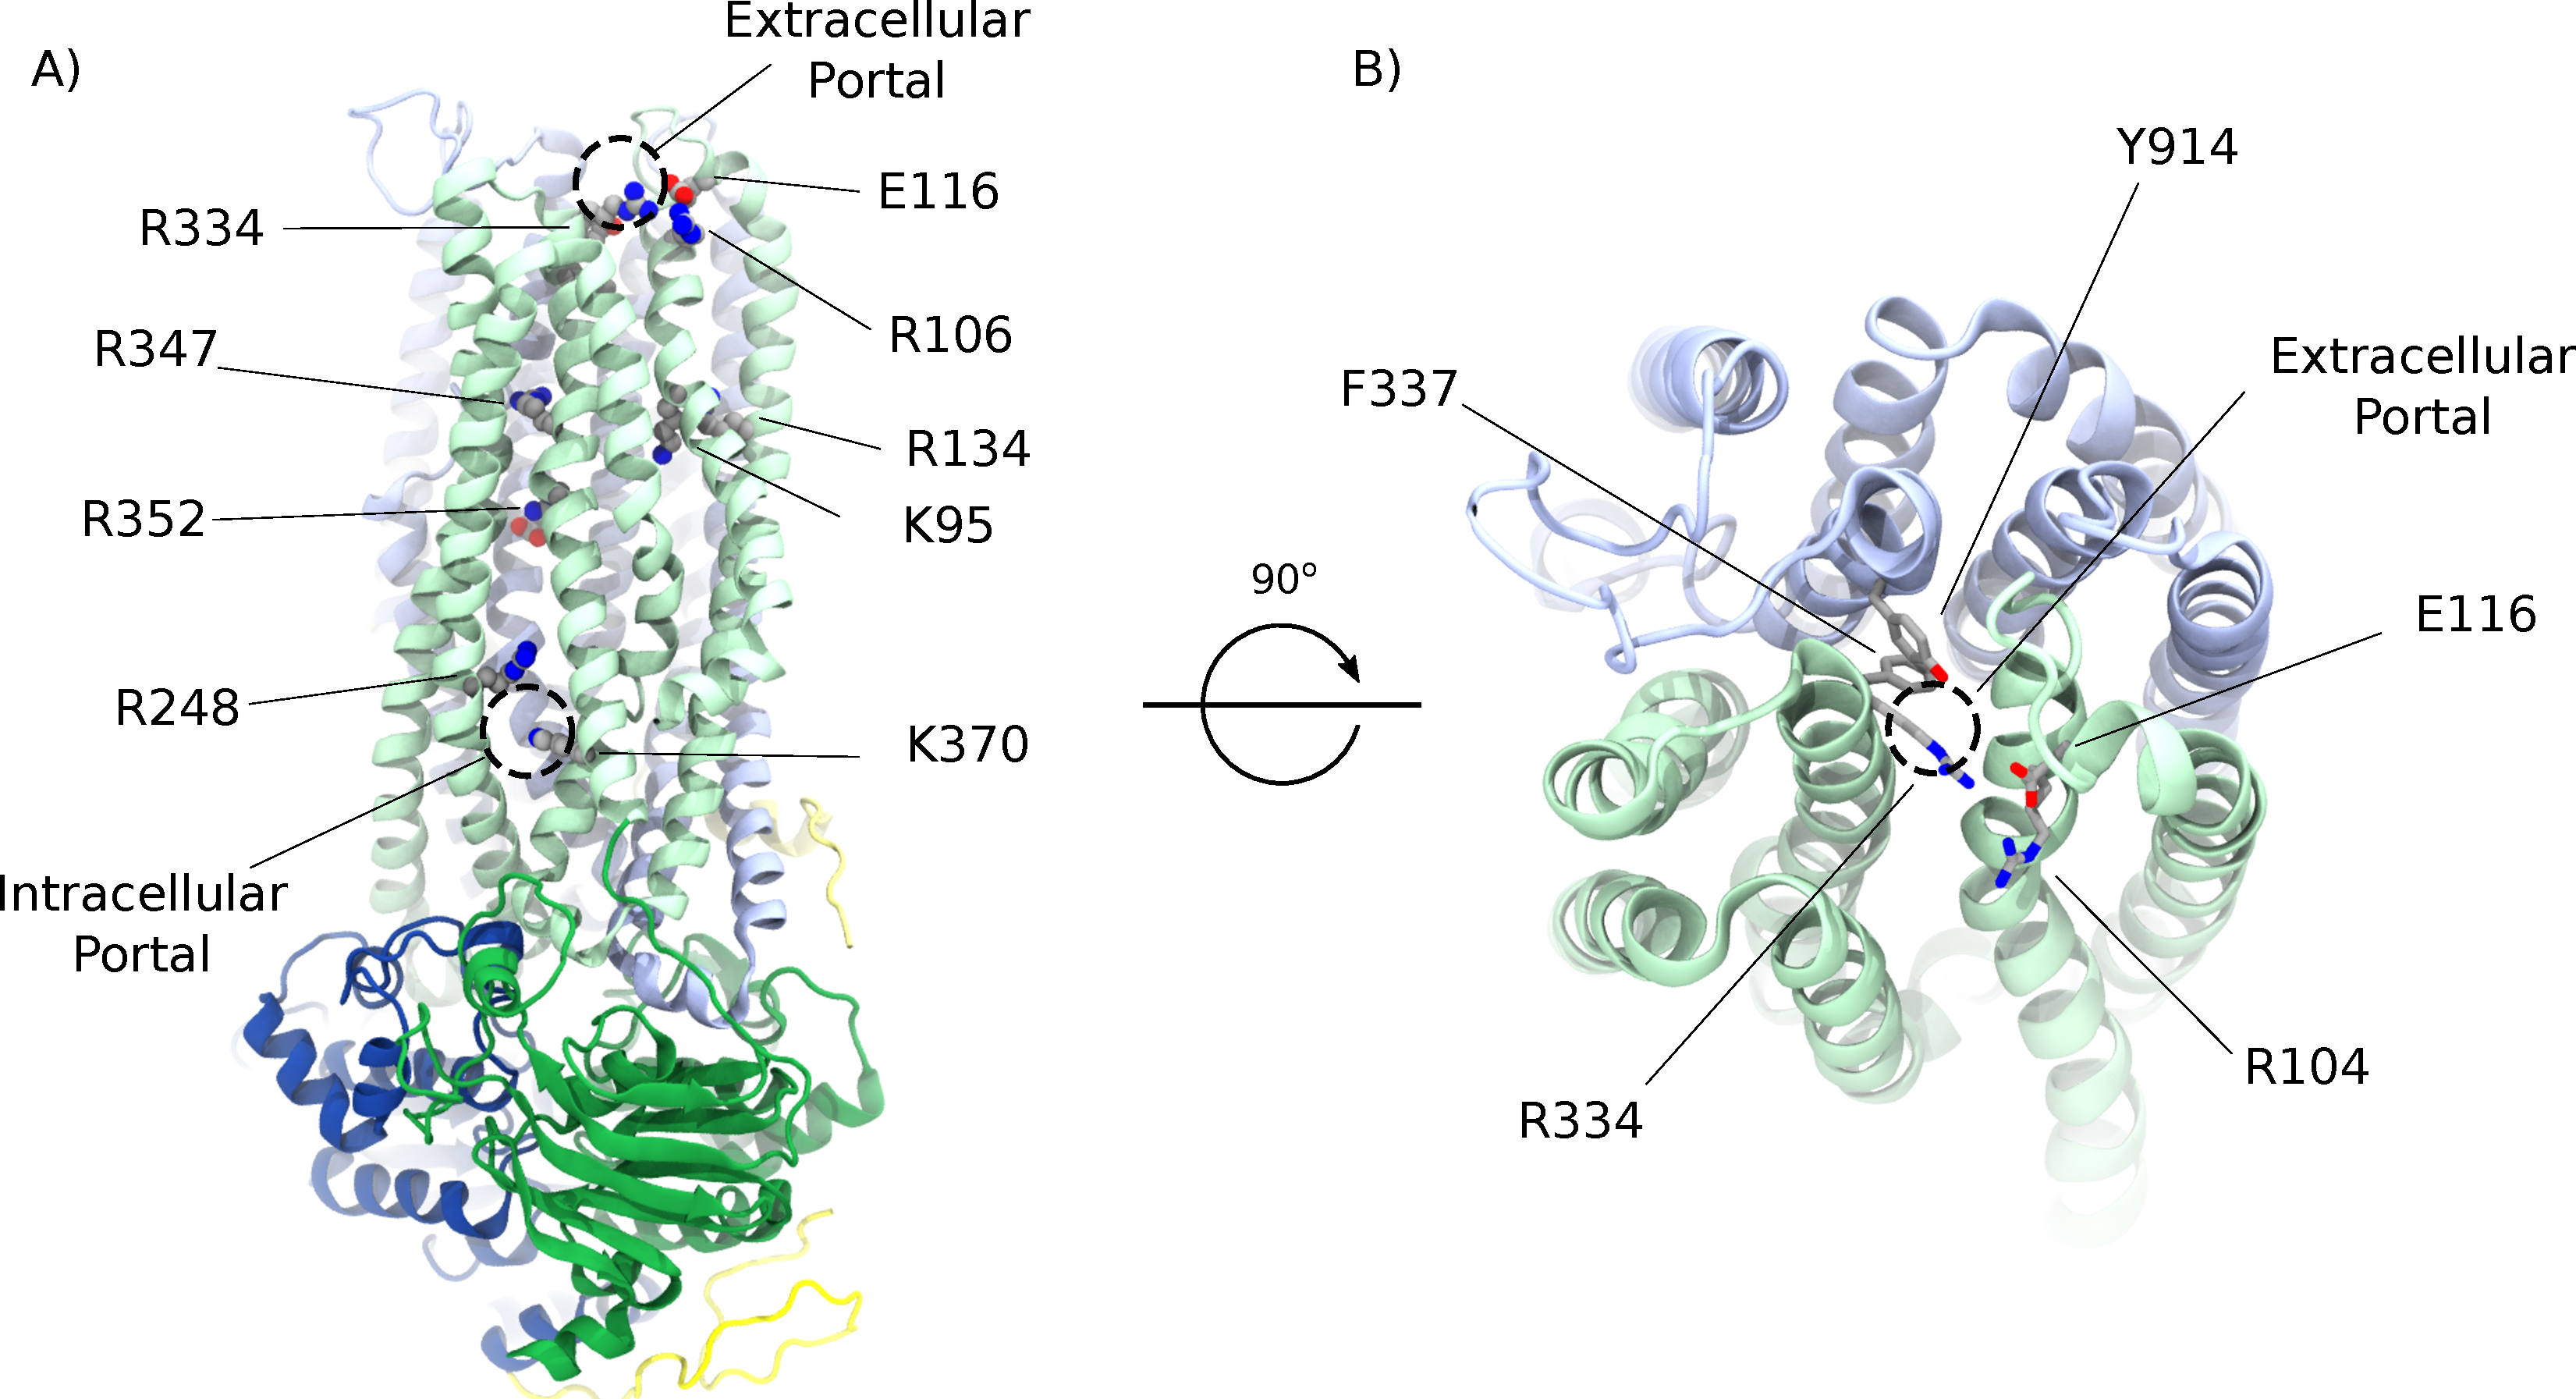
\includegraphics[width=\textwidth]{figures/chloride_passage_figure.pdf}
	\end{center}
	\captionsetup{singlelinecheck = false, justification=raggedright}
	\caption[Chloride Passage through CFTR] {\textbf{Chloride Passage Through CFTR}}{A)Ions enter through an intracellular gate, which is lined with positive amino acids. The subsequent inner vestibule is also lined with amino acids which chloride loosely associates with as it moves through the channel. B) A top down view of the extracellular portal. We have highlighted some hydrophobic amino acids which play important roles in the selectivity of anions. Pictured is the only available structure of the activated human CFTR channel \cite{zhang2018}. Unfortunately, this conformation is not sufficiently open to conduct ions. We will analyse an open conformation in chapter \ref{chap:opening} which we predicted through simulations.} 
	\label{chloride_passage}

\end{figure}

CFTR will permeate cations but there are a set of anions which it will conduct. The conduction pathway of the channel can be split into two regions. The inner vestibule which is wide and covered with basic, positively charged amino acids and the selectivity filter which is formed by the narrowing of the protein in the upper part of the channel. These regions are hotspots for disease causing  mutations, with most mutations occurring on TM6 in TMD1 (Figures \ref{CFTR_mutations_pie_chart} and \ref{chloride_passage}) \cite{cftr2}.

F337 is the most important amino acid for selectivity, with the F337A mutation leading to an increase in conductivity and a loss in selectivity \cite{wei2016}. Bicarbonate (HCO$_3^-$ is known to have roughly 25\% the permeability of chloride through the channel\cite{tang2009}. Some interaction partners such as WNK1 have been shown to influence the selectivity of the channel \cite{kim2019, garnett2011, kim2019a}. The permeation of bicarbonate is very important physiologically. If a CF-causing mutation permeates bicarbonate, there is a high likelihood the patient will be pancreatic sufficient. Increasing bicarbonate secretion is being explored as a possible therapeutic strategy \cite{ferrera2021}. 

Compared to cation channels like Gramicidin and KcsA, CFTR is only weakly selective---permeating a large set of anions with varying radii and geometries (Figure \ref{chloride_passage}) \cite{linsdell1998, tabcharani1997, poulsen1994}. CFTR appears to act like other anion channels where lyotropic (low solvation energy) anions pass more easily than kosmotropic anions (high solvation energy). This would suggest that partial dehydration of the anions is likely during conductance \cite{linsdell2000}. The radius of a dehydrated chloride ion is 1.7$\AA$ while a hydrated chloride ion has a radius of 3.2$\AA$ \cite{yang2002}. As noted in its source publication, the 6MSM structure which we have studied has a constriction of 1.2$\AA$ at its narrowest point. Hence, even if chloride were to be fully dehydrated during conduction, there would have to be some level of conformational change in the protein. This was the motivation for the extensive free energy calculations undertaken in chapter \ref{chap:opening}.

\subsection{Different classes of Cystic Fibrosis Phenotype}
As the above shows, CFTR is a complex protein which can misfunction in a number of ways. Based on the way the mutation presents in \textit{in vitro} assays, disease causing mutations are classified into 6 common classes. Ultimately, the aim of this thesis is to demonstrate that that at the atomic level, there is much more nuance to these classes, and a mutation can have features of multiple classes at the same time.

This has important implications for the treatment of the disease. Due to the heterogeneity between patient responses to therapies, there is a growing interest in personalising the treatment of disease and mapping the molecular effects of mutations can inform this process of theratyping \cite{crawford2018,sette2021}. As patient specific treatment evolves, these classes will likely become less relevant, serving as illustrative tools only to communicate at a higher level what is going wrong with the CFTR protein. The specific choice of treatment will depend on a number of personal factors. The canonical classification is as follows:

\begin{figure}
	\begin{center}
	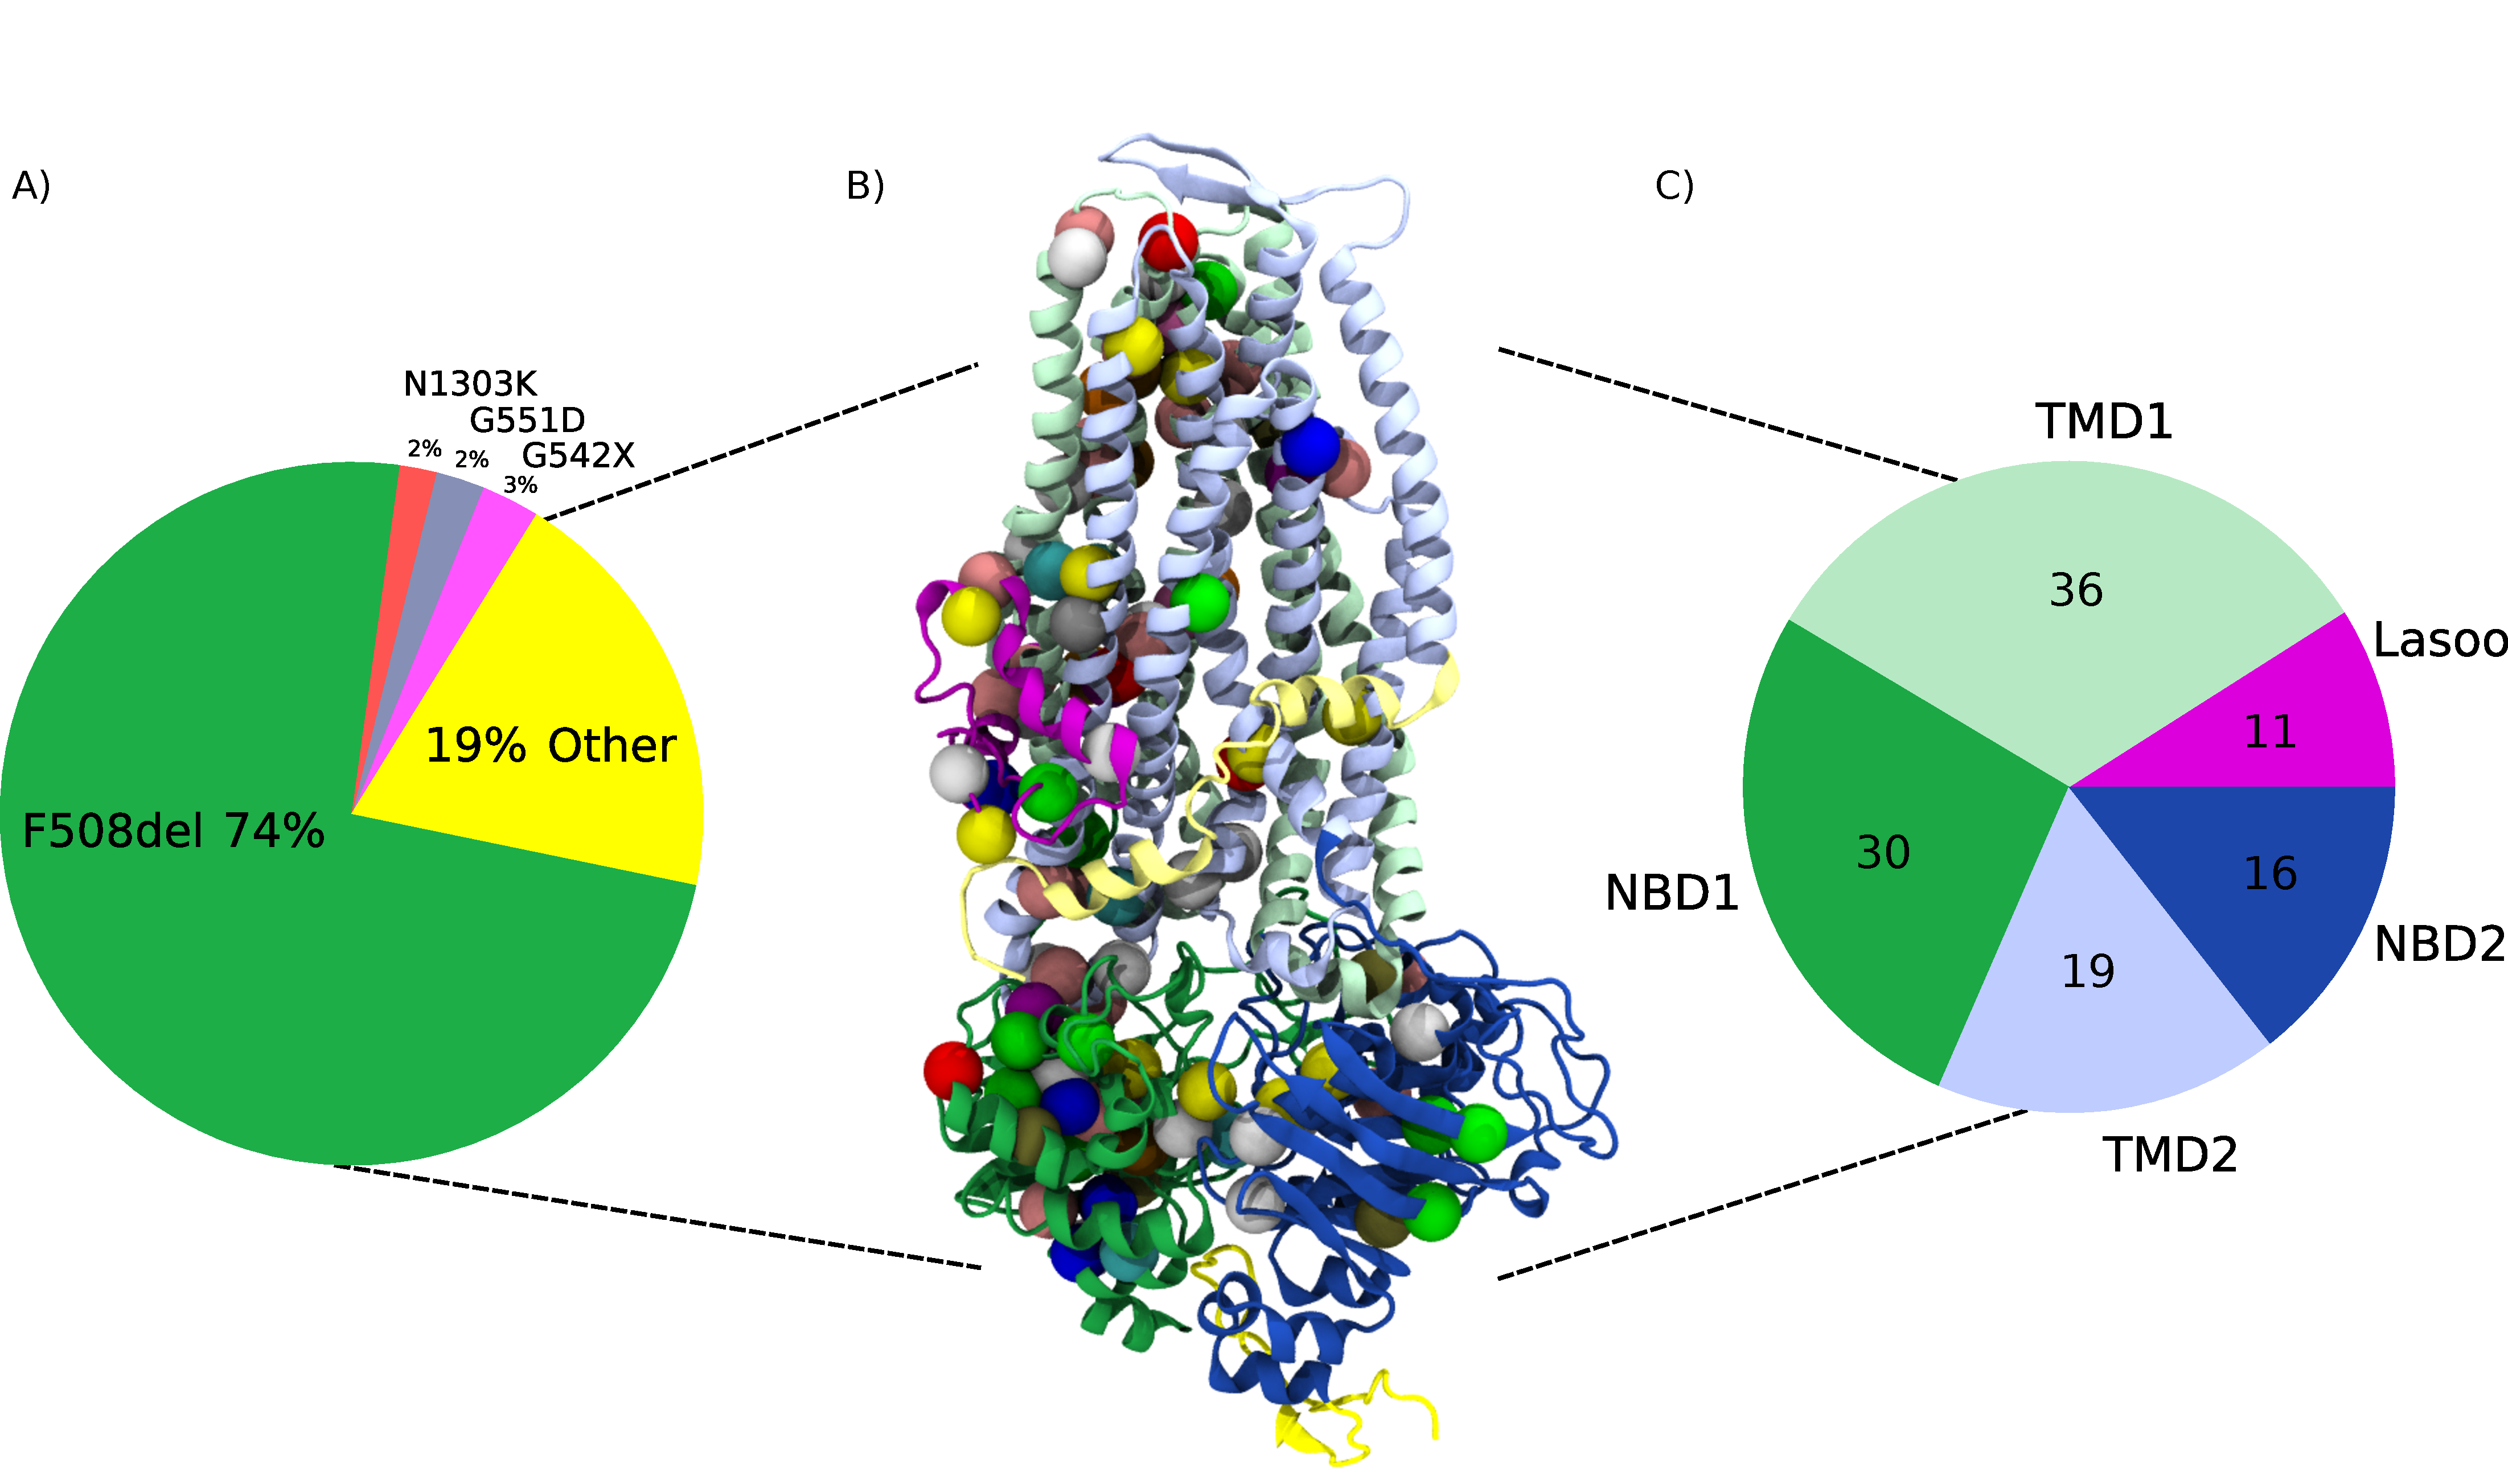
\includegraphics[width=\textwidth]{figures/alleles_pie_chart.pdf}
	\end{center}
	\captionsetup{singlelinecheck = false, justification=raggedright}
	\caption[Rare Mutations Occur in Across the CFTR Protein] {\textbf{Rare Mutations Occur in All parts of the CFTR Protein}}{A) The reported frequency of all disease causing alleles (not just missense mutations) in the CFTR2 database. At the time of writing there are 402 recorded different disease causing mujtations. A patient with CF will carry two of these mutations. 1 in 25 people of Northern European descent are a carrier for CF and are themselves at increased risk for many health problems \cite{ioannou2014, miller2020}. B) The location of all 112 known disease causing missense mutations mapped on the CFTR protein itself as spheres. In addition to those visualised here there are many of variants of unknown significance (VUS) which may cause disease but are so rare they have not been clinically studied. C) The incidence of CF causing missense mutations in the different domains of the CFTR protein. TMD1 and NBD1 have the highest concentration of disease causing mutations. Likely due to the former's role in ion permeation and the latter's role in gating \cite{cftr2}}. There are no confirmed CF causing missense mutations in the C-terminus or the R-domain. As patient registries are set up across the world it is likely that more rare CF causing mutations will be discovered in the future. \footnote{Note that in this figure we have included the novel I37R mutation studied in this thesis. This mutation has not yet been recorded in CFTR2.} 
	\label{CFTR_mutations_pie_chart}
\end{figure}


\begin{itemize}

	\item \textbf{Class I} No functional protein. Under these mutations no protein is transcribed due to either problems with the transcription of mRNA or a premature stop codon truncating protein synthesis early, meaning the resulting peptide is missing key domains. 
	\item \textbf{Class II} Folding defect. These mutations cause the translated peptide to misfold into the incorrect tertiary structure. This can inhibit the protein's journey as it is trafficked to the cell membrane. 
	\item \textbf{Class III} Impaired Gating. Here the mutation inhibits the ability of the protein to transition from the closed to the open state. 
	\item \textbf{Class IV} Decreased Conductance. These mutations cause a barrier in the energy landscape of the CFTR chloride conductance pathway.
	\item \textbf{Class V} Less Expressed Protein.  
	\item \textbf{Class VI} Decreased Functional Lifetime

\end{itemize}

Although useful from a clinical and experimental standpoint, in reality, these classes do not reflect the molecular nature of a mutaiton. Mutations may in fact belong to many categories at once, to differing degrees. This has lead to a more granular approach in more recent literature \cite{veit2016}. In particular, through this thesis we will demonstrate that membership of one of these classes can be due to a range of molecular phenotypes. Hence, this classification is becoming increasingly outdated and there is a need to understand the unique, sometimes overlapping, molecular phenotypes of each mutation. Further, through our molecular simulations we will see that in fact CFTR modulators appear capable of treating many different mutations with unique modes of pathogenesis. This is the purpose of chapters \ref{chap:I37R}-\ref{chap:opening}. In each chapter we will analyse a specific mutation in detail and then use \textit {in vitro} techniques to demonstrate that the molecular defect introduced by the mutation can be rescued by existing CFTR modulators. 

A molecular understanding has previously been outlined for certain mutations, though rarely with the advantage of the full hCFTR structure or extensive statistical sampling. For example, \cite{belmonte2015} based their modelling on SAV1866 and used short unbiased simulations as well as simple free energy estimates in order to demonstrate the deleterious nature of the G551D and $\Delta$F508 mutations. This is remarkably consistent with the findings of more recent studies which have the benefit of more structural information about the protein \cite{bahia2021}. This latter study used isolated structures of NBD1 and 2 (PDB IDs: 2PZE \cite{atwell2010} and 6UK1 \cite {wang_2020_nbd2_CFTR_isoalted_pdb_alone} respectively) in order to predict the $\Delta\Delta G$ change to the folding energy of CFTR from disease causing mutations. The authors correlated their results with \textit{in silico} prediction functions from Rosetta and find remarkable agreement. Although this study does not shed light on molecular details of misfunction, it will likely be a critical resource for the grouping of theratype. 

To date, there are two studies which have used a similar approach to us to study mutations. They also attempted to understand the molecular defects of rare mutations \textit{in silico} and then combining these findings with patient specific platforms to demonstrate their rescue by CFTR modulators. The first of these studies used the zCFTR structure, in order to study the ultra-rare W361R mutation \cite{billet2020}. Here, the authors found that a lipid tail binds into a hydrophobic pocket formed by the W361 amino acid. This lead to the expectation that the W361R mutation would cause a class II folding defect. Unfortunately, the authors did not explicitly simulate the effects of the W361R mutation, though the nature of the folding defect they would expect to see is likely not accessible on simulation time scales.

A second study addressed the intriguing mutation P67L on the lasso motif \cite{sabusap2021}. This mutation occurs in a hotspot of CF-causing mutations and also in the vicinity of corrector type drugs \cite{gene2008, fiedorczuk2022}. Here, the authors were able to rely on the structure of activated hCFTR to  a change in NBD2. However, the simulation methodology in this paper is questionable. The authors simulated hCFTR for less than 200ns and claim to have discovered allostery between the lasso motif and NBD2. Such an effect would likely take orders of magnitude more simulation time to observe because of the distance between these domains in the simulated structure. The simple statistical test employed by this paper in Figure 7, on a single simulation replicate, is also not fit for purpose \cite{knapp2018}. However, the pharmacological and biochemical results from this publication are certainly extremely successful in shedding light on the molecular nature of this mutation.

Although the authors of these works have seen the deleterious effects of mutations through simulations and demonstrated their rescue with pharmaceuticals, these prior studies are not as rigorous as the work we have undertaken for this thesis. None of these studies simulated CFTR for more than 1 microsecond and none of them have employed free energy calculations. However, these study validate the approach we will use for subsequent chapters and further, allow us to demonstrate the power of using MD and free energy calculations as computational microscopes to investigate CFTR misfunction. 

Similar to the above, the defects we will explore in each chapter are largely unique: 

\begin{itemize}
	\item \textbf{I37R} is a mutation which occurs on the lasso motif. In chapter \ref{chap:I37R} we explored how this novel mutation causes a class III gating defect by giving rise to a pathogenic interaction with a fragment of the R-domain. This fragment was poorly resolved in the cryo-EM structure of CFTR and we first had to identify it using MD. Our structural predictions were then confirmed upon the release of Alphafold2 \cite{jumper2021}.  

	\item \textbf{R352Q} deletes a positive charge on TM6, along the chloride conduction pathway in the inner vestibule. In chapter \ref{chap:R352Q} we used umbrella sampling and unbiased MD to demonstrate the misregulation of the conduction pathway in this mutation. Demonstrating a class IV conductance defect. 

	\item \textbf{S945L} occurs in TM8 on TMD2. In chapter \ref{chap:S945L} we discovered a stable network of hydrogen bonds which links S945 to Y852 on the R-domain. We hypothesised that the replacement of the polar serine sidechain with hydrophobic leucine might cause a perturbation to this section of the R-domain. Due to the kinetic barrier from the surrounding lipids we again employed umbrella sampling to explore how the perturbations this mutation causes to the R-domain causes both a folding and a gating defect.

	\item \textbf {R334W} occurs at the extracellular pore, at the end of the selectivity filter on TM6 in TMD1. In chapter \ref{chap:opening} we used multiple walker OPES-metadynamics in order to dilate the existing structure of human CFTR (PDB ID: 6MSM) and study the effects of the R334W mutation on chloride conductance.

\end{itemize} 


Through our MD simulations, we found that each of these rare mutations has a unique molecular fingerprint. They appear to cause CFTR to misfunction in unrelated ways. Further, in each of these cases, we have either presented \textit{in vitro} patient specific assays or surveyed the literature to demonstrate that pharmacological rescue of these rare mutations is possible using CFTR modulators \cite{R334W_Euro_CF_trial}.  It is then remarkable that these unique molecular modes of pathogenesis all to respond to CFTR modulators. It is these results which inform the conclusions in chapter \ref{chap:conclusion}, where identify directions for further studies of CFTR and argue that many patients who are currently excluded from access to modulator therapy are likely to benefit from these life changing drugs. 

%FIGURE demonstrates how each of the canonical classes at the molecular level is broken down into many sub classes and a mutation might belong to one of many of these subclasses. Structural biology paradigms and \textit{in silico} modelling can help classify mutations into these different classes. In combination with wet lab assays we can understand which classes of these molecular defects are most effectively treated with specific drug regimens. Our computational microscope is helping choose treatments for patients at the atomic level. 

\section{Modulators Act Directly on CFTR to Restore its Function}
\begin{figure}
	\label{drugs_bound}
	\begin{center}
		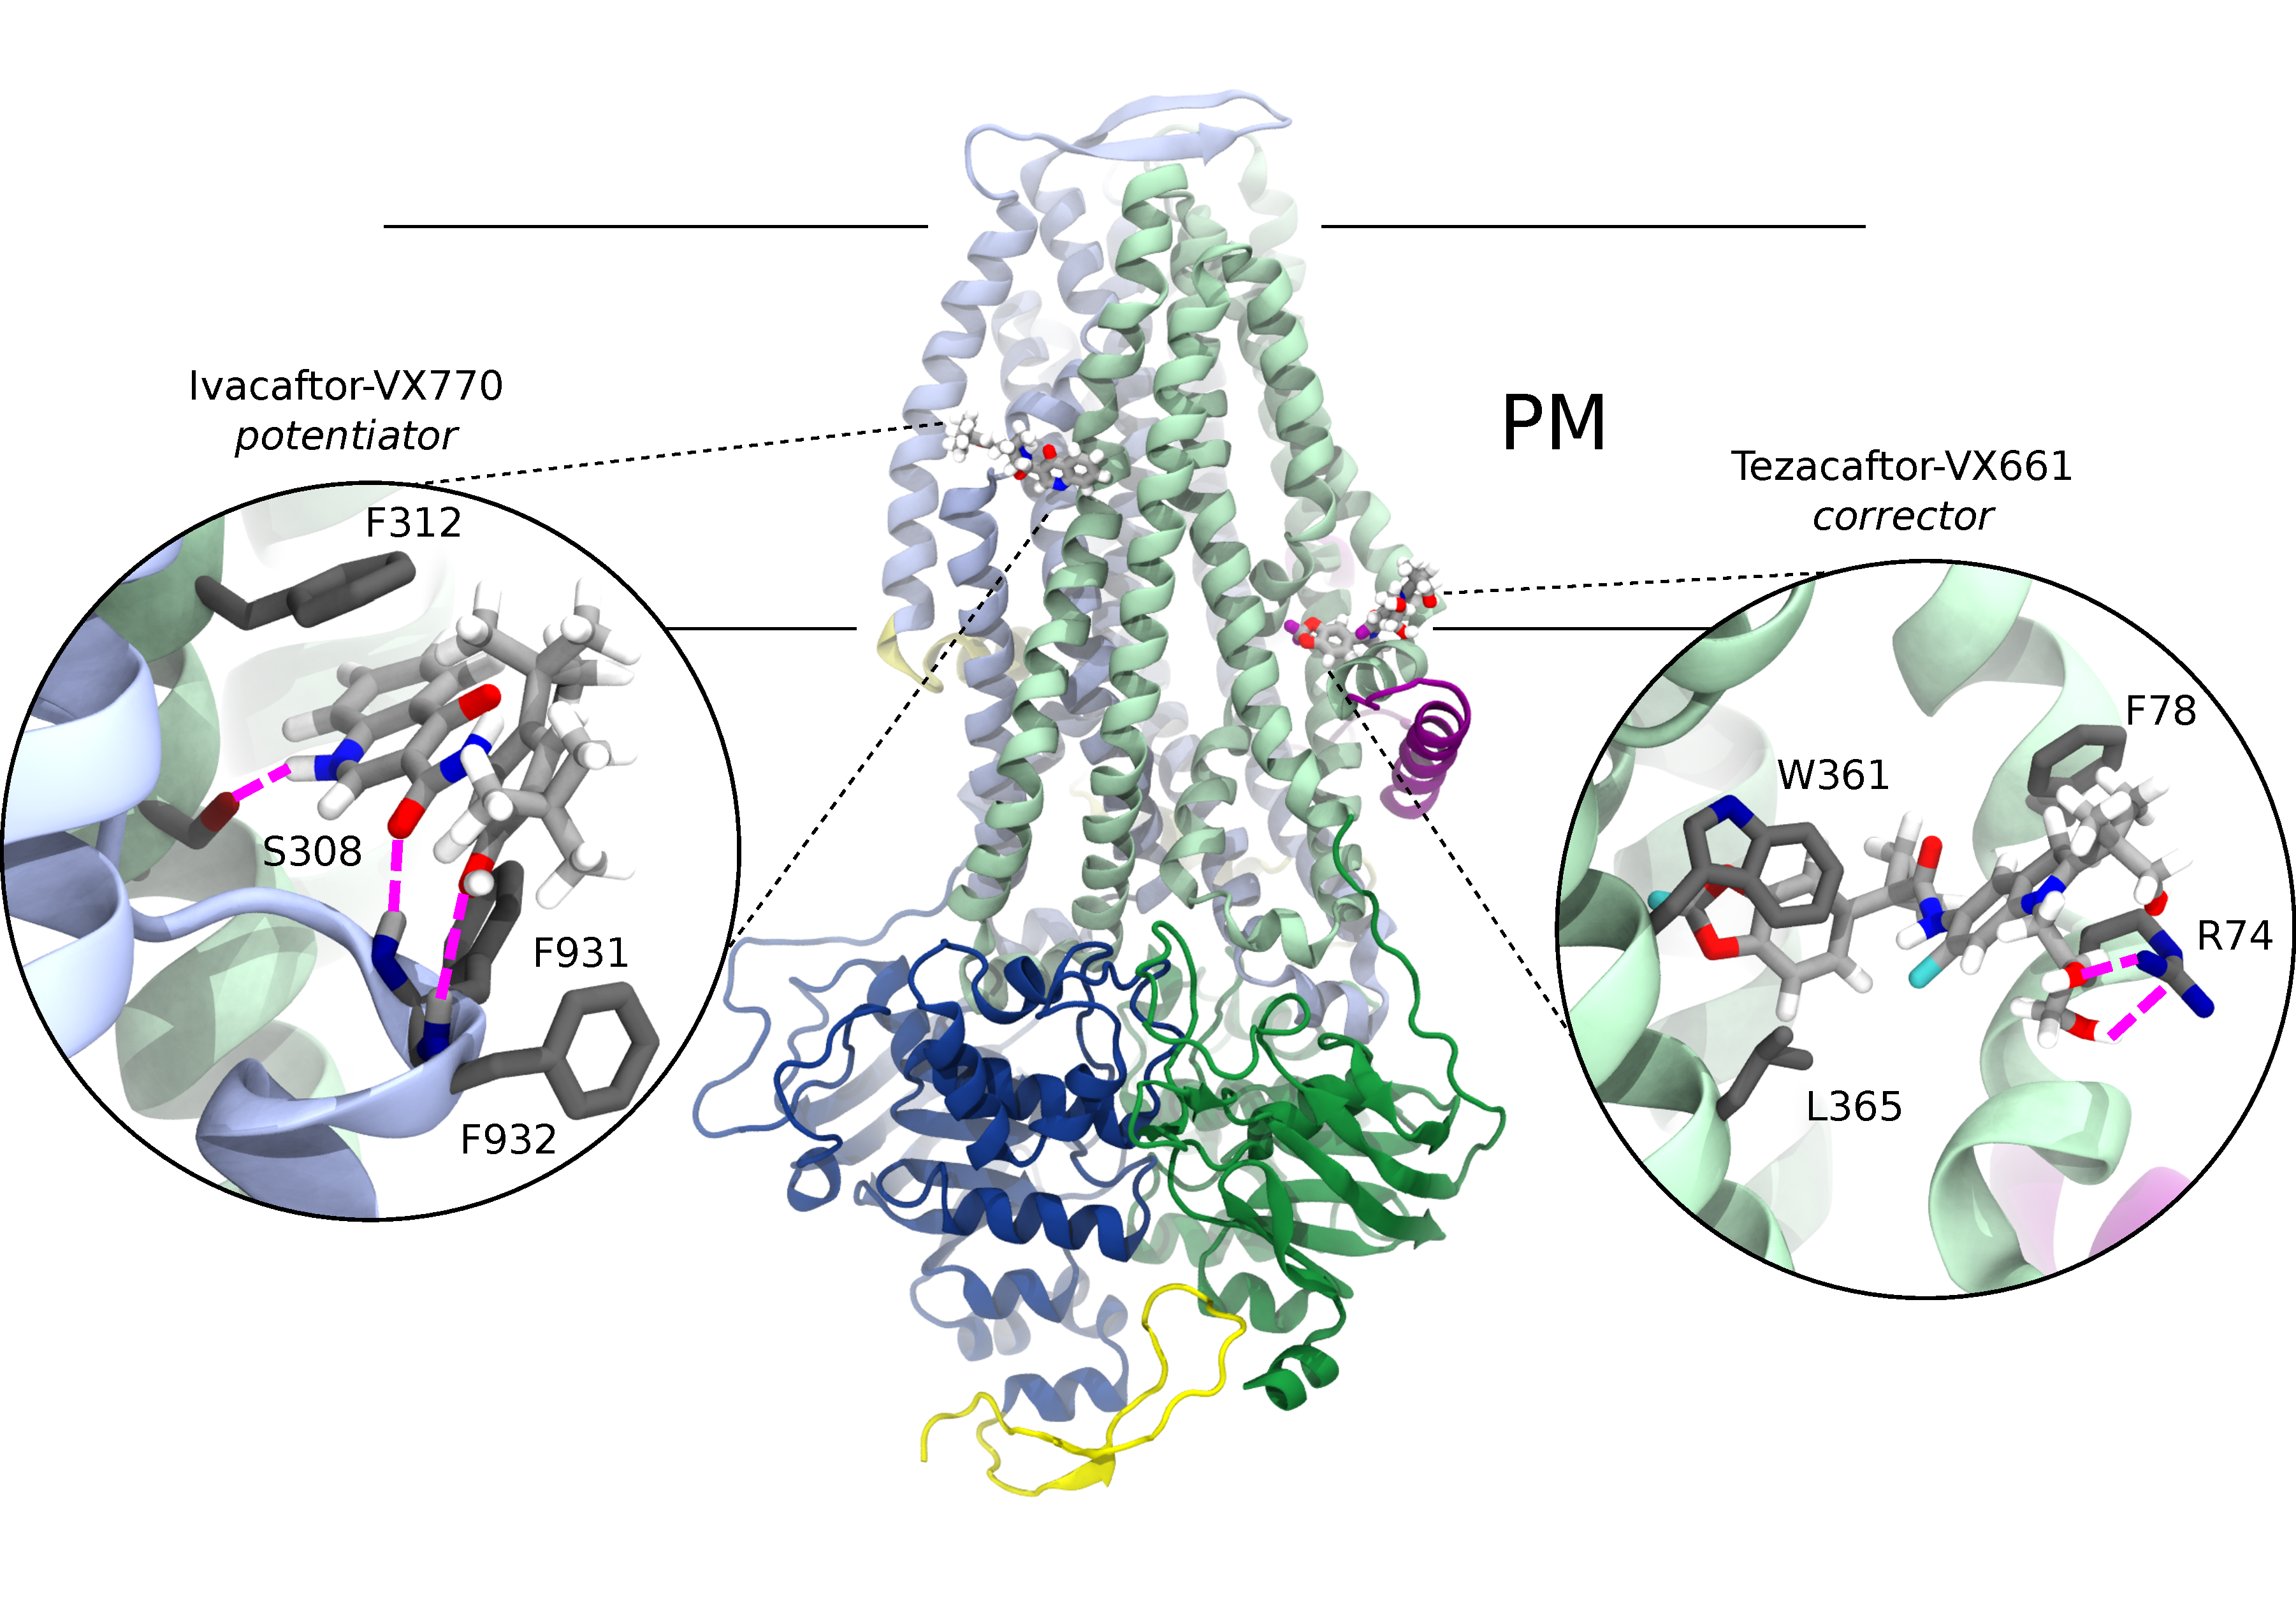
\includegraphics[width=1\textwidth]{figures/drugs_bound_overall.pdf}
	\end{center}
	\captionsetup{singlelinecheck = false, justification=raggedright}
	\caption[Modulators Bound to CFTR] {\textbf{Modulators Bound to CFTR}}{The structurally imaged binding sites of potentiators and type I correctors \cite{liu2019, fiedorczuk2022}. Potentiators in particular are proposed to bind to other sites as well \cite{yeh2019, liu2019}. Hydrogen bonds are labelled with purple dotted lines. Note how both visualised binding sites require substantial contributions from the surrounding lipid bilayer. The presence of these lipids will play an important role in the binding kinetics and energetics of these drugs \cite{csanady2019}. Future molecular studies should account for these nuances.} 
\end{figure}

Since CFTR is at the heart of CF pathogenesis, it has been pursued for decades as target for therapeutics. Through high throughput \textit{in vitro} screening, four compounds which act directly on CFTR have been clinically approved for the treatment of CF. These drugs are known as CFTR modulators. They fall into two categories. Correctors, which aid CFTR to fold into the correct state and potentiators which help the channel reach the fully open state once it has folded correctly and integrated into the membrane. Since their discovery, several \textit {in vitro} biophysical experiments have investigated the mechanism of action and binding site of these compounds \cite{csanady2019,  laselva2022, yeh2017, yeh2019, fiedorczuk2022, krainer2018}. 

Due to the excitement surrounding these compounds, there have been a few simple \textit{in silico} studies of CFTR modulators\cite{molinski2018, bitam2021, baatallah2021, froux2020}. When not performed carefully, \textit{in silico} docking studies for small molecules may produce very crude and inaccurate findings, this was particularly apparent when reviewing the large number of docking studies performed during the coronavirus pandemic of 2020-2022 \cite{gimeno2019, derek_lowe_virtual_screening_2022, ceron-carrasco2022}. It is then fortunate that previous MD and docking studies of CFTR modulators have been largely consistent with subsequent structural and biochemical experiments \cite{liu2019, scientifique2019, yeh2019, yeh2017, fiedorczuk2022}. Even though these studies are limited in the impact of their findings, their success can be attributed to the close integration of these \textit{in silico} techniques with biochemical assays. This would indicate some promise for the approach of this thesis and future \textit{in silico} studies of CFTR which, will hopefully have access to even more computational power and structural information. 

%Recently, cryo-EM structures of many of these compounds in their bound state have been published \cite{liu2019, fiedorczuk2022}. 

An added benefit of modulator therapy is that they have have demonstrated promise in improving not just the most acute symptoms of CF (lung function), but they may be able to treat or even relieve deleterious CF associated complications. In some cases, modulators have been found to relieve pancreatic insufficiency and CF related diabetes \cite{gaines2021,lopes-pacheco2020, yi2021} and there is ongoing ongoing study into the possible benefits of modulators on bacterial infections \cite{harvey2022}. This highlights the importance of treating the root cause of a disease when we are presented the opportunity and not just its symptoms. 

\subsection{Correctors}
Corrector class modulators are able to treat Class II folding defects. The most common type of correctors are known as type I correctors, which help the CFTR protein fold into the correct structure by binding to a hydrophobic pocket in TMD1 formed by TMs 1, 3, 4 and 6. This binding mode has been directly visualised by cryo-EM imaging with atomic resolution \cite{fiedorczuk2022}. This binding mode was expected, as circular dichromism \cite{greenfield2006} and fluorescence experiments found that an isolated construct of TMH3 and TMH4 were more likely to fold correctly in a model membrane in the presence of corrector compounds \cite{krainer2018}. 

In combination, these studies give us a strong base to understand the mechanism of action for corrector compounds. The correctors tezacaftor (VX-661) and elexacaftor (VX-445) form two components of the triple therapy Trikafta \cite{administration2021, trikafta_website}. Tezacaftor is a type I corrector while elexacaftor has been found to have some potentiation capacity on CFTR, leading it to be classified as a type III corrector. A review of all types of correctors can be found in \cite{veit2018}. Further work will aid in the creation of new compounds to refine our exploitation of current correction strategies.

\subsection{Potentiators}
Potentiator class drugs bind to CFTR in order to increase the number of channels which are conducting chloride in the cell at any one time. This helps to balance osmotic pressure over the epithelium and relieve symptoms \cite{fda_kalydeco_2_years_or_older, fda_kalydeco_approval, jih2013,yeh2017}. However is some uncertainty surrounding the molecular details of their mechanism of action. 

There is consensus that potentiators bind directly directly to CFTR, in order to increase the likelihood that the channel occupies a conducting state. Indeed, some potentiators such as VX-770 (ivacaftor), which forms the third component of Trikafta, rescues CFTR with picomolar affinity \cite{csanady2019}. 

Controversy arises surrounding precisely \textit{where} these drugs are binding in order to rescue CFTR. Different studies discovering different binding sites for the same drugs, via mutagenesis and other methods \cite{yeh2019, liu2019, laselva2021}.  

Careful investigation of different potentiator molecules give hints as to the solution to these problems. For example, GLPG1837 has not been approved in a clinical setting but through \textit {in vitro} experiments it has been demonstrated that it is more efficacious at potentiating CFTR even though it has lower affinity for the CFTR protein itself \cite{vanderplas2018}. This would indicate that the highest affinity binding pocket does not produce the greatest modulation. 

More work is needed to resolve the mechanism which results in the highest clinical effectiveness of these drugs. These disagreements are closely related to the kinked conformation of TM8, where they are proposed to bind \cite{liu2019, yeh2019}. Some of these issues will be addressed in more detail in chapter \ref{chap:conclusion} where we will suggest some \textit{in silico} strategies to address them. 

The competitive nature of certain potentiator and corrector drugs opens the possibility that specific genetic defects may be optimally rescued by specific combinations and doses of both correctors and potentiators compounds \cite{csanady2019}. This means there may be much to gain from the patient specific approach like the one employed for this thesis. 

The elucidation of the binding site for potentiators has been attempted with unbiased MD using the hCFTR structure (6MSM) \cite{laselva2021}. This study used an octanol slab as well as a model POPC membrane in order to accelerate the diffusion of VX-770 in the transmembrane portions of CFTR. With 10 $\mu$s of unbiased MD sampling, the authors discover 7 binding poses for the potentiator drug. The authors combine their results with a photo-label and mass spectrometry results which will likely play a critical role in future drug development of potentiators. They use these innovative toosl to conclude that both a site on ICL4 and the site visualised by cryo-EM experiments play a role in potentiating CFTR activity. This is consistent with other \textit{in vitro} experiments \cite{csanady2019}.

Unfortunately, in this study, none of the binding sites observed \textit{in silico} corresponded to the binding mode visualised by cryo-EM experiments \cite{liu2019}. The authors speculate that this may be because the cryo-EM site is in fact low affinity but it is likely that even though 10 $\mu$s is represents a considerable investment of computational resources, it is simply not enough sampling to see ligand binding and unbinding. The kinetics of a membrane facing drug binding site occur on the order of milliseconds \cite{weikl2016}. Hence, free energy calculations would be needed for such an endeavour and we will propose such a study in chapter \ref{chap:conclusion}. 

\subsubsection{Read Through Compounds}
Roughly 10\% of known disease causing mutations result in a premature stop codon in the mRNA of the CFTR gene. This means protein synthesis is stopped early, and the resulting protein will be missing critical domains. 

Since there is no full length CFTR protein synthesised by cells carrying this mutation, potentiators and correctors are unable to directly assist. This has lead to the need to develop a class of drugs known as read through compounds which allow the continued synthesis of the protein, past the premature stop codon \cite{sharma2021}. At the time of writing no read through compounds have been clinically approved but efficacy has been demonstrated in pre-clinical models \cite{crawford2021}. Since correctors and potentiators also modulate the behaviour of WT-CFTR it is likely that correctors and potentiators would be given in combination with read through compounds and other therapies as a complimentary treatment.

\subsubsection{Alternative and Complimentary therapeutic Strategies}
As the root cause of disease, CFTR will continue to be an important therapeutic target. However, there will also be increasing value in the therapeutic benefit derived from manipulating other protein systems---both as complimentary a strategy to the modulation of CFTR and to the treatment of complications. This is especially pertinent when we consider that some patients do not respond to CFTR modulators, even when they share the genotype of patients who do. These patients would benefit greatly from complimentary therapeutics \cite{hanafin2021, robertson2015, lingam2017, seelig2020, barbieri2021a, grebert2019}. 

As mentioned in section \ref{clinical_realities_CF}, one of the most troublesome complications of CF is the chronic infection experienced by patients. Unfortunately, modulators have not been able to reliably alleviate this complication \cite{mallapaty2022}. This is because these bacterial colonies a protective biofilm and thus become very difficult to eradicate with traditional antibiotics. To this end, bacteriophage therapies are being pursued as a complimentary strategy to those above \cite{ng2021}. 

There is also exciting work on gene and cell based therapies to directly deliver properly functioning CFTR proteins into the bodies of CF patients \cite{allan2021}. This is being investigated through the use of different advanced vectors, such as the retro virus lentivirus. With these vectors, WT-CFTR is usually added \textit{ex vivo} and then the treated cells are transplanted back into the patient. However, it may may soon be possible to edit the genome of a CF-afflicted embryo and cure the patient before they are even born using a system like Crispr-Cas9 \cite{ledford2020}. This latter technique has been misused in the past \cite{mallapaty2022} and the reader is again referred to section \ref{cftr_lit_review_intro} for texts on bioethics. 

\section{Patients with Rare Mutations Struggle to Access Modulator Therapy}
CFTR modulators have proven to be a breakthrough in the treatment of CF. However, there is strong motivation behind our focus on rare mutations in this thesis. Roughly 50\% of Cystic Fibrosis cases are caused by a homozygous mutation, $\Delta$F508, and 90\% of patients carry at least one copy of this mutation. At the time of writing, many jurisdictions such as Australia and the EU have approved a drug combination therapy known as Trikafta for patients carrying one copy of $\Delta$F508. Given that these drugs act directly on CFTR, we would expect that mutations may also respond to triple therapy. 

Thus, the exclusion by regulators of patients with rare mutations leaves a significant part of the CF afflicted population without access to this life saving medication, with many more excluded due to the extreme cost of the drugs themselves \cite{administration2021, trikafta_website, abdallah2021, guo2022a}. 

Traditional clinical trials are also not possible for many of these rare mutations, as there may not be enough patients carrying one mutation to study them in the same trial \cite{grody2007}. Hence, we aim to demonstrate that a larger section of the CF population is likely to respond to modulators, particularly those carrying missense mutations. Eventually this work will contribute to a clinical method known as theratyping, where a granular understanding of CF pathogenesis will allow a personalised choice of treatment.

The treatment of rare mutations has particular significance in CF. Not only would patients be otherwise left behind, but by studying rare mutations, outcomes can be improved for all people with CF. For example, potentiator class drugs were discovered by high throughput molecular screening against the rare class III gating mutation G551D \cite{vangoor2009}. By studying rare mutations we can gain a more complete understanding of the nature of the disease and so improve therapies for everybody. This approach will become more important in the future as CF is uncovered in regions where it is rarer. In these populations there is also a broader spectrum of CFTR mutations, meaning patients in these regions are more likely to have a rare form of disease \cite{singh2015,zheng2017,ni2022}. As patient registries are launched in these populations, we will discover more rare forms of CF. This expected trajectory of CF epidemiology makes the approach of this thesis critical, such that all people with CF can benefit from the advances being made by translational research \cite{zheng2017, garcia2022}. 


%Patients with rare forms of CF are more likely to be in countries where CF is already quite rare \cite{zheng2017}. Patients on modulators have significantly different clinical outcomes even between those with the same genotype. Determining the reason for this would open the door to the development of complimentary therapeutics. 

The earlier patients are able to benefit from modulator therapy, the better their prognosis \cite{lahiri2022}. It is also well documented that patients with the same genotype may respond differently to the same modulators \cite{hanafin2021}. Hence, by validating a patient specific approach to rare mutations we can build a platform to choose the right modulators for all patient. Considering that patients with the same genotypes often respond differently to the same modulators, it is critical that more modulators and complimentary therapies are developed, to give all patients more options and better outcomes \cite{hanafin2021}.

\section{Patient Derived Organoids: A Pre-Clinical Model to Assess Modulators}
In chapter \ref{chap:methods} we constructed a model based on interacting atoms to study biomolecular systems. Similar to this philosophy, medical researchers also seek model systems to understand the function of organs. In CF research, this has lead to the development of techniques where samples of epithelial stem cells are taken from patients and grown into structures which mimic the function of either the lung or the gut \cite{wong2015,depoel2020}. These are known as patient derived organoids.

This is possible due to a population of adult stem cells which live in the epithelium. These cells maintain their ability to differentiate into a variety of cell types (a property known as pluripotency) \cite{blanpain2007}. 

To grow organoids, epithelial stem cells are scraped from a patient's nasal passages or taken during a rectal biopsy. These samples can be used to grow either lung or intestinal organoids respectively  \cite{awatade2021,sato2011}. The morphology of the organoids can be confirmed through immunofluorescence microscopy \cite{awatade2021, im2019}. Organoids are excellent model systems, but like all models, they are incomplete. They often lack specialized cell types and miss much of the complexity which might arise from interactions with other organs \cite{clevers2016}. 

However, these models have the potential to be a powerful supplement to traditional studies which would normally involve enrolling patients in clinical trials \cite{pranke2019a}. Organoid models then have the potential overcome a complex, bureaucratic and time consuming barrier to patient care.

Adult stem cells in the epithelium are preferable to other sources of stem cells. This is because other sources which might be easier to harvest, such as iPSCs from the skin or white blood cells, would require complex, time consuming protocols to grow into organoids \cite{wong2012}. Already, the differentiation and expansion of epithelial samples into the organoids studied here takes one month \cite{sato2011}.

In the case of CF, this technology allows the construction of a scalable, patient specific platform where the response of a patient's own tissues can be tested to determine their response to a given treatment \cite{keegan2021, sato2011}. 

It is hoped that these pre-clinical models will allow more patients with rare CF causing mutations to access modulators. This has given rise to an exciting prospect of a practice known as theratyping, enabling clinicians to make a personalised prediction of which therapies will best serve a patient \cite{clancy2019, wong2022, wong2022a, ciciriello2022}. This thesis demonstrates that integration of \textit{in silico} simulations into the process of theratyping can further the predictive power gained from the use of these \textit{ex vivo} models.

%One limitation of these organoid platforms is the lack of an inflammatory response since no immune cells are present in the tissue culture. 

Subsequent chapters will make use of these organoids by testing them with a set of \textit{in vitro} assays in order to characterise a patient's response to modulator therapy. For the physicist reader, a brief explanation of these assays is given below.

\subsection{Forskolin Induced Swelling to Assess CFTR Function}

\begin{figure}
	\label{FIS_figure}
	\begin{center}
	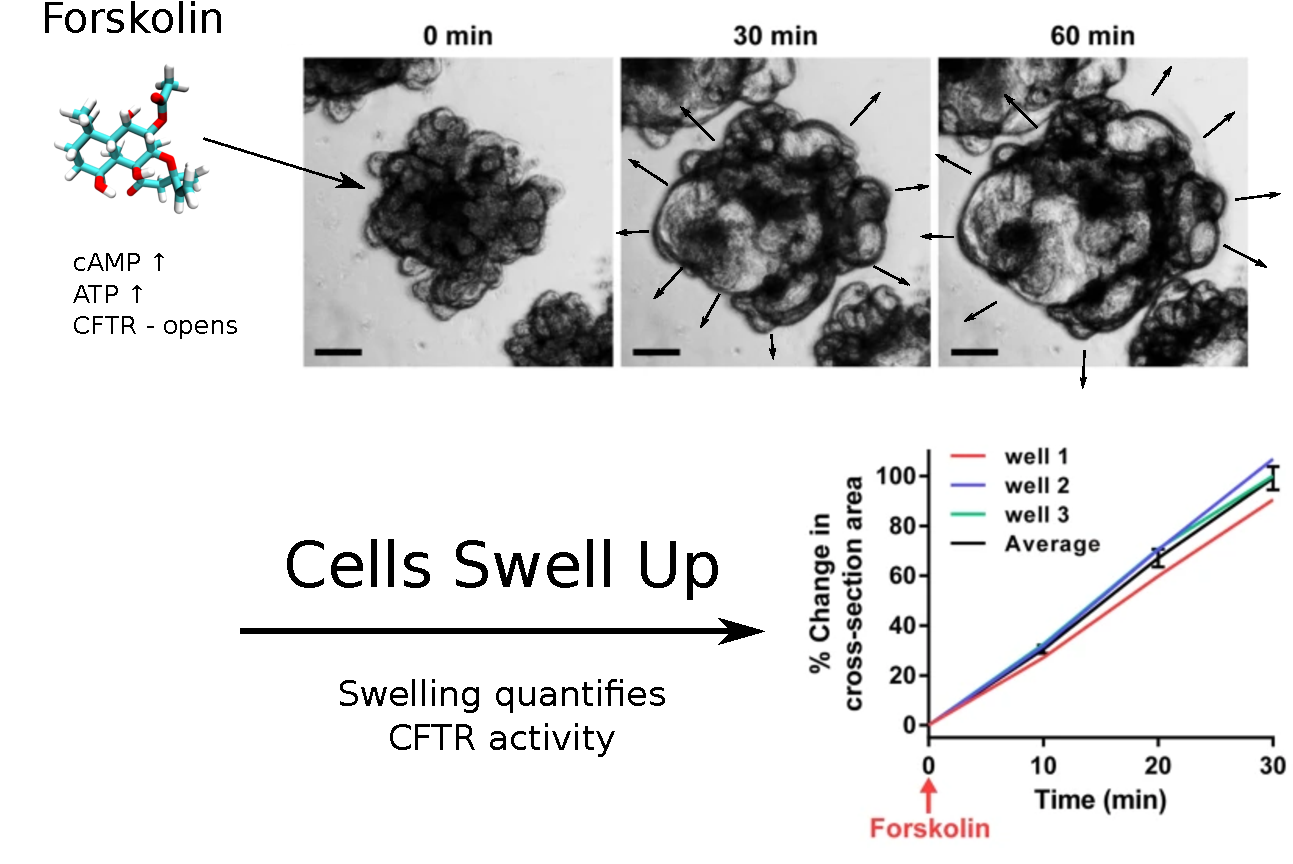
\includegraphics[width=1\textwidth]{figures/FIS_demo.pdf}
	\end{center}
	\captionsetup{singlelinecheck = false, justification=raggedright}
	\caption[Forskolin Induced Swelling] {\textbf{Forskolin Induced Swelling}}{Upon exposure to Forskolin, epithelial cells begin to produce cAMP. This causes an increase in intracellular ATP which will open CFTR channels. The influx of water into the cell causes them to swell. The amount of swelling can be used to quantify the amount of properly functioning CFTR in the cell.} 
\end{figure}
Forskolin Induced Swelling (FIS) assays can be used used to easily characterise the amount of functioning CFTR in a patients cells \cite{dekkers2013}. When epithelial cells are exposed to a chemical known as forskolin they begin to rapidly produce cyclic AMP (cAMP, a precursor to ATP in a cell) \cite{bonora2012}. The presence of ATP activates the CFTR ion channels, causing the cells themselves to swell due to the intake of moisture. When performed under a micropsope with patient derived orgnaoids, this swelling allows cell biologists to easily quantify the activity of CFTR within a cell in a variety of conditions, such as the presence of drugs.

Hence, by comparing the amount of swelling swelling of organoids in the presence or absence of modulators, we can quantitatively assess the response of a patient's cells to modulator therapy (Figure \ref{FIS_figure}). 

\subsection{Electrophysiology Directly Measures CFTR Gating and Conduction}
The measurement of electrical activity in biological systems is known as electrophysiology. This field has been an important way for us to develop models for the activity of ion channels and the cells which host them \cite{aidley1996}. Since CFTR is an ion channel, measuring its electrical activity is a direct way to assess its function and dynamics, leading to a molecular understanding of the nature of disease. 

In order to study the action of a single ion channel one needs to employ an experimental technique known as patch clamp electrophysiology \cite{hille2001}. Studies using this technique were vital for the conclusions of chapters \ref{chap:R352Q} and \ref{chap:opening}. On the other hand, to assess the competency of a whole membrane or tissue, one instead uses what is known as an Ussing chamber. 

\subsubsection{Patch Clamp Electrophysiology}
\begin{figure}
	\begin{center}
	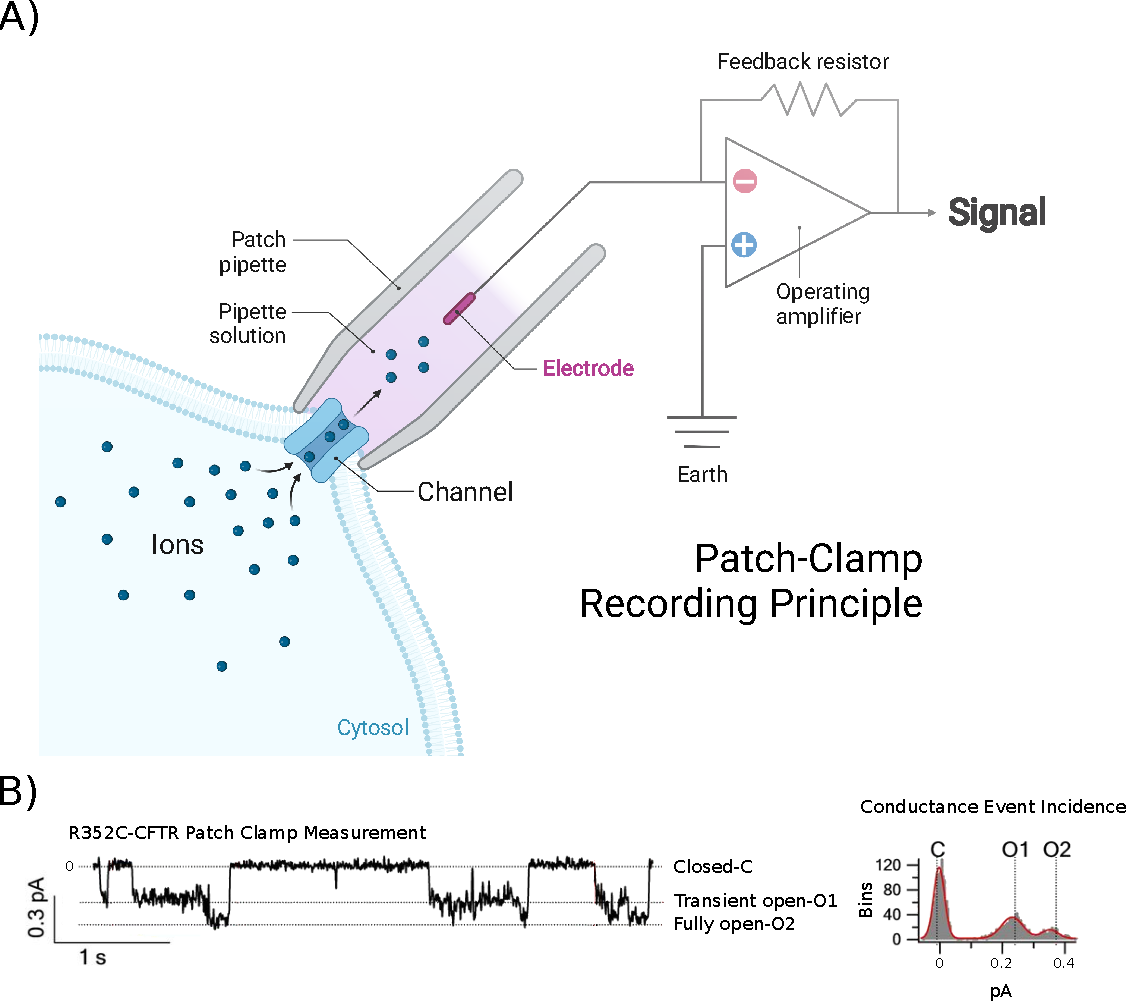
\includegraphics[width=0.8\textwidth]{figures/R352C_ephys_measurement_figure.pdf}
	\end{center}
	\captionsetup{singlelinecheck = false, justification=raggedright}
	\caption[Patch Clamp Apparatus] {\textbf{Patch Clamp Apparatus}}{A) In patch clamp electrophysiology, a micropipette is placed against the membrane to create a tight seal \cite{patch_clamp_recording_principal_figure}. B) The current trace from the measurement of a mutant CFTR channel. The R352C mutant was chosen for visualisation as it shows a clearly shows two open states: a transient state with lower conductance, known as the O1 state and a fully open state known as the O2 state \cite{jih2012}. The accidental discovery of this mutant has been used extensively in studying the gating cycle of CFTR, giving an interesting example an example of how useful electrophysiology can be for molecular biophysics. Source data from \cite{jih2012}. Note that this mutant has roughly half the conductance of WT-CFTR.} 
	\label{patch_clamp}
\end{figure}

Patch Clamp Electrophysiology has been critical to the development of molecular biophysics in ion channels. Through the use of a micropipette filled with electrolyte solution, we can measure the activity of a single ion channel. As shown in figure \ref{patch_clamp}, the tip of a micropipette is placed directly on a cell membrane in order to measure the current flowing through a single ion channel. A single ion channel exhibits a current on the order of 1 picoAmp (for reference, CFTR exhibits 0.7pA at a bias voltage of 100 mV), so the formation of a tight seal with the membrane is critical to filter out noise. To tighten this seal, a small amount of suction is usually applied to the membrane through the pipette \cite{aidley1996}.

In the inside-out variant of this technique, the ion channel along with a small patch of membrane is excised, exposing the system to the surrounding bath. This means that the response of the ion channel to different chemical conditions can be tested by changing the composition of the bath. Patch clamp electrophysiology experiments are not presented in this thesis but they considered closely when writing chapter \ref{chap:opening}  so an outline of them has been given here.

\subsubsection{Ussing Chambers}
An Ussing chamber is a versatile apparatus which allows the measurement of current across an epithelial membrane. In chapters \ref{chap:I37R}, \ref{chap:R352Q} and \ref{chap:S945L}, they were used extensively. Here, a mono-layer was derived from an organoid and used as a patch in the Ussing chamber. By blocking other ion channels such as ENaC during measurements, a clear picture of CFTR function can be measured in order to create an understanding of the nature of disease in each patient. The monolayer could also be exposed to different regimens of modulators in order to assess the ability of those modulators to rescue the function of the organoid. The higher the current, the more CFTR proteins were functioning and the better the rescue of the mutation.

In Ussing chamber measurements, current is usually expressed as amps per unit area, which normalises the measurement to the size of the patch. It is also important that the patch of epithelial membrane is continuous, as holes would allow current to pass unrestricted give errantly high readings. This highlights how great care must be taken when growing organoids. 


\begin{figure}
	\label{ussing_chamber}
	\begin{center}
	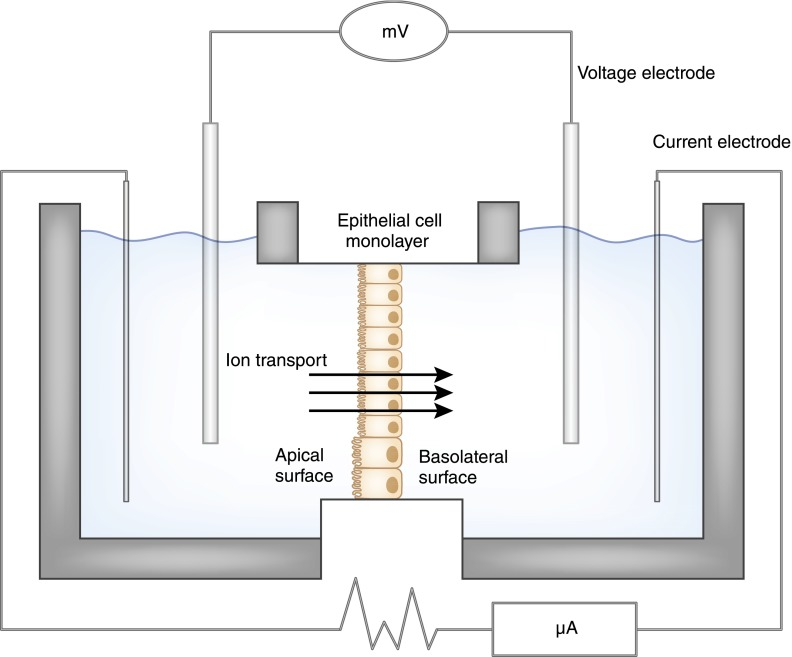
\includegraphics[width=0.4\textwidth]{figures/ussing_chamber.jpg}
	\end{center}
	\captionsetup{singlelinecheck = false, justification=raggedright}
	\caption[Ussing Chamber Setup] {\textbf{Ussing Chamber Setup}}{Ussing chambers can be used to characterise the function of an epithelial monolayer. The membrane can be exposed to different cellular conditions and its conductance can be measured under these conditions to test different drugs. For our purposes, an Ussing chamber may be used to measure the ion transport of an epithelium grown from a patient derived organoid. Source \cite{hoenig2014}} 
\end{figure}


\subsection{Western Blotting Assesses CFTR Trafficking}
\begin{figure}
	\label{western_blot}
	\begin{center}
	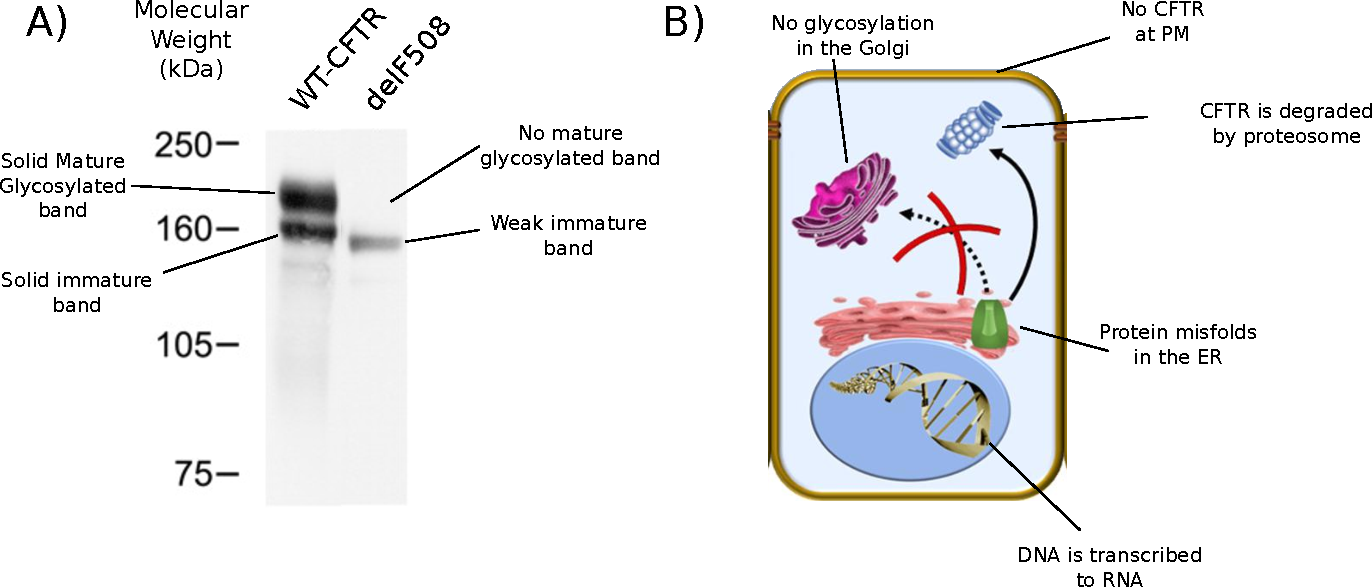
\includegraphics[width=1\textwidth]{figures/western_blot_explanation.pdf}
	\end{center}
	\captionsetup{singlelinecheck = false, justification=raggedright}
	\caption[Western Blot Explanation] {\textbf{Western Blot Explanation}}{A) Output of a western blot experiment. WT-CFTR has much more abundant protein than $\Delta$F508 \cite{chang2008}. B) The cell biology behind why the $\Delta$F508 mutation is pathogenic. When WT-CFTR folds correctly in the Endoplasmic reticulum it is trafficked into the Golgi where it is glycosylated, before it is then implanted into the cell membrane. In the case of $\Delta$F508, the protein misfolds as it is synthesised, so instead of being trafficked as normal it is prematurely degraded by the proteosome \cite{lopes-pacheco2016a, lewis2005}.} 
\end{figure}
The above methods focus on measuring the electrical activity of the ion channels once they are at the cell membrane, they will only detect functional channels. In order to test the presence of ion channels within the epithelium, functional or otherwise, a technique called western blotting is employed (Figure \ref{western_blot}).

A simplified explanation of the most common technique is given below but there are many variations
\begin{enumerate}
	\item The proteins in the sample of cells are denatured, sometimes by boiling. This makes them unfold and stretch out into long peptides. 
	\item The proteins in the sample are injected into an agar gel.
	\item The gel is immersed in a buffer solution and a voltage is applied to it in a process known as electrophoresis. This causes proteins to migrate through the gel according to their charge to mass ratio. The heavier the protein, the less it will move. 
	\item The presence of proteins is visualised through immunostaining. First, the gel is washed with a primary antibody. This antibody is specific protein we wish to detect (in our case, CFTR). 
	\item The excess primary antibody is washed off the gel, but some of the antibodies will stay bound to the proteins we are interested in. 
	\item A secondary antibody is washed over the gel. This is engineered to bind to the primary antibody. What is important about the secondary antibody is that it is attached to a special enzyme tag, which we can visualise.  
	\item The excess secondary antibody is washed off the gel, but but some of the secondary antibodies will remain bound to the primary antibody.
	\item The tag on the secondary antibody is visualised through the use of chemiluminesence. The tag is typically an enzyme, which emits light when it breaks down a substrate. Hence, for the visualisation step, a photographic film is placed over the gel and it is washed a final time, in the substrate of the enzyme which the secondary antibody is attached to. This produces bands in the photographic film, the darker the band is at position, and the more of the target is present there.
\end{enumerate}
By washing the gel in different primary antibodies, we can detect multiple proteins in one experiment. This is often used to normalise the quantity protein measured between samples. Hence, one will often see structural proteins such as tubulin or actin in figures showing the results from a western blot. These are used as controls and should not change due to between experiments. Western blotting is thus a simple, widely used technique to quantify the amount of specific proteins in the cell. 

\section{Conclusion}

Note throughout the chapters ahead how we have relied on results from careful biochemical and biophysical literature which elucidated the molecular details of the function and misfunction of CFTR. Close reading of these studies was necessary in order to form hypothesise about the function of CFTR which we could test \textit {in silico}. 

In biophysics, it is only through the collection of \textit{in vitro} data through which we can formulate our theoretical models. So we are grateful for the painstaking work of Paul Linsdell, Christine E. Bear, Robert Ford, Laszslo Csandy, Tzyh-Chang Hwang, Naels Mccarty, Isabelle Callebaut, John Paul Mornon, David Gadsby, Jue Chen, Ina Urbatsch, John Hunt, Julie D. Foreman Kay and all the members of their laboratories for their detailed studies of the CFTR protein. This is not to discount the work which went into the identification of the CFTR gene \cite{riordan1989}, nor the outstanding work of the clinicians and physicians who work with patients to understand more about the nature of the disease \cite{roberts1957}.  

As was mentioned in the \href{Foreword} {\ref{chap:foreword}}, experts from many fields must all work together to understand the whole organism and thanks to decades of work by hundreds of people we have a host of molecular details which we can combine in order to understand the function and misfunction of CFTR. In the next 4 chapters we will combine some of these details, alongside our own findings from organoid studies and simulations to make our own contribution to the molecular understanding of Cystic Fibrosis as a disease. This literature will again be used for our conclusion in chapter \ref{chap:conclusion} to push for certain questions to be answered in molecular CF research.

CFTR is just one protein. It's a complicated one to be sure but it's far from the most complicated in a mammalian cell \cite{saotome2018, zalk2015, chen2018a}. I hope that this chapter has given an appreciation of the level of detail that exists in biological systems. Remember that there are an estimated 42 million individual protein molecules in each cell, in more than 20 thousand variates \cite{ho2018, salzberg2018}. The decades of insight into CFTR was motivated by the terrible disease it is responsible for, but this also gives us the opportunity to demonstrate the power and insight gained from a molecular understanding of disease. The next 4 chapters will be examples how to combine the simulations we looked at in chapter \ref{chap:methods} with insights from patient specific assays, to understand more about CF pathogenesis. These results will be tied together in chapter \ref{chap:conclusion} to help us understand \textit{how} drugs are rescuing CFTR function and the direction this conclusion would suggest for research into treating the root cause of CF.


%=======================================================================================%
\chapter{Molecular Dynamics and Functional Characterization of I37R-CFTR Lasso Mutation Provide Insights into Channel Gating Activity}
\label{chap:I37R}
\chapquote{My name is Benjamin John Goodwin} {-Benjamin John Goodwin (personal communication)}

\section*{\centering Abstract} 

Characterization of I37R, a mutation located in the lasso motif of the CFTR chloride channel, was conducted by theratyping several CFTR modulators from both potentiator and corrector classes. Intestinal current measurements in rectal biopsies, forskolin-induced swelling (FIS) in intestinal organoids, and short circuit current measurements in organoid-derived monolayers from an individual with I37R/F508del CFTR genotype demonstrated that the I37R-CFTR results in a residual function defect amenable to treatment with potentiators and type III, but not type I, correctors. Molecular dynamics of I37R using an extended model of the phosphorylated, ATP-bound human CFTR identified an altered lasso motif conformation which results in an unfavorable strengthening of the interactions between the lasso motif, the regulatory (R) domain, and the transmembrane domain 2 (TMD2). Structural and functional characterization of the I37R-CFTR mutation increases understanding of CFTR channel regulation and provides a potential pathway to expand drug access to CF patients with ultra-rare genotypes.\\

\smallskip

\begin{figure*} [h]
	\begin{center}
		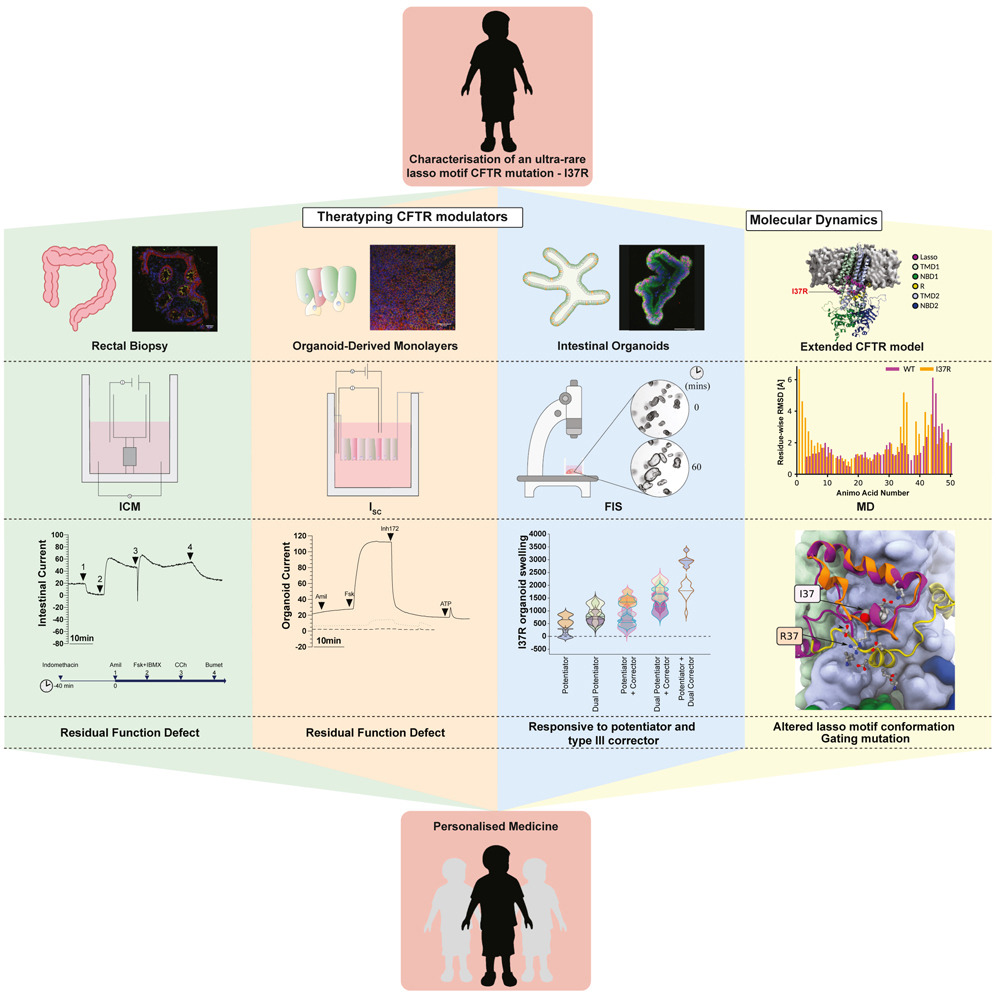
\includegraphics[width=0.80\textwidth]{figures/I37R/graphical_abstract.jpg}
	\end{center}
	\captionsetup{singlelinecheck = false, justification=raggedright}
	\caption[Graphical Abstract. Integration of in silico and in vitro experiments for personalised medicine] {\textbf{Graphical Abstract. Integration of in silico and in vitro experiments for personalised medicine}}{}
	\label{I37R_graphical_abstract}
\end{figure*}

\section{Introduction}
Cystic fibrosis (CF) is a life-limiting genetic disease resulting from mutations in the CF transmembrane conductance regulator (CFTR) gene \cite{ratjen2015}. CFTR—the only member of the ABC transporter family known to be an ion channel—consists of two transmembrane domains (TMD1 and TMD2) which form an anion-selective pore, two highly conserved nucleotide-binding domains (NBD1 and NBD2) with ATP-binding pockets and a newly described N-terminal lasso motif \cite{hwang2013, zhang2016}. In addition, CFTR has a unique, disordered regulatory (R) domain which contains protein kinase A (PKA) phosphorylation sites. For the CFTR channel to open and close (gate), cAMP-dependent PKA phosphorylation of the R domain first activates the CFTR (\cite{gadsby1994}). Then, ATP-binding induces the dimerization of the two NBDs which opens the channel pore and ATP hydrolysis closes the pore.

The lasso motif (amino acids (aa) M1-L69), which is partially embedded in the bilayer and interacts with the R domain, was recently resolved following advancements in cryo-electron microscopy (cryo-EM) of the CFTR structure \cite{liu2017, zhang2018a}. The first 40 amino acids of the lasso motif, which include lasso helix 1 (Lh1, aa V11–R29), form a circular “noose” structure \cite{Hoffmann2018}. The noose structure wraps around the transmembrane helices (TM2, TM6 of TMD1 and TM10, TM11 of TMD2) and is held in place by hydrophobic interactions with L15, F16, F17, T20, L24, and Y28. The C-terminal end of the lasso, which includes the lasso helix 2 (Lh2, aa A46–L61), is tucked under the elbow helix (aa I70–R75) \cite{Hoffmann2018}. Variable disease severity and heterogeneous clinical presentation have been reported for the 78 CFTR variants identified so far in the lasso motif (CFTR1 and CFTR2 databases, Table S1). Evidently, the lasso motif has a multifunctional role in CFTR regulation with variants impacting folding, gating, and stability of the CFTR protein \cite{fu2001, gene2008, jurkuvenaite2006, sabusap2021, thelin2007}.

CFTR modulators, small molecules which directly target CFTR dysfunction, are now available to certain individuals with CF. Currently, two classes are approved; (1) potentiators, which open the channel pore such as ivacaftor (VX-770) and (2) correctors, which assist CFTR protein folding and delivery to the cell membrane. Type I correctors (lumacaftor/VX-809, tezacaftor/VX-661) stabilize the NBD1-TMD1 and/or NBD1-TMD2 interface by binding directly to TMD1 \cite{loo2013, ren2013} or NBD1 which improves the interaction between NBD1 and the intracellular loops \cite{loo2017, hudson2017}. Type II correctors (C4) stabilize NBD2 and its interface with other CFTR domains while type III correctors (elexacaftor/VX-445) directly stabilize NBD1 \cite{okiyoneda2013}. Combination therapies of corrector(s) and a potentiator (Orkambi, Symdeko/Symkevi, Trikafta/Kaftrio) have been approved for CF individuals with F508del, the most common CFTR mutation, as well as several specific residual function mutations. Most recently, Trikafta/Kaftrio has been approved for patients with a single F508del mutation in combination with a minimal function mutation, broadening the population of patients with CF eligible for treatment with CFTR modulator therapy.

Mounting evidence has shown that in vitro functional studies in patient-derived cell models successfully predict clinical benefit of available CFTR modulators for individuals bearing ultra-rare mutations \cite{berkers2019, mccarthy2018, ramalho2021}. In individuals with CF, adult stem cells are usually collected by taking either airway brushings or rectal biopsies. Single Lgr5+ stem cells, derived from crypts within a patient's intestinal epithelium, can be expanded in culture medium and differentiated into organized multicellular structures complete with the donor patient's genetic mutation(s), thus representing the individual patient \cite{sato2009}. Stem cell models can be used for personalized drug screening to theratype and characterize rare CFTR mutations \cite{awatade2018, berkers2019, pollard2018}. Determining the functional response of rare, uncharacterized CFTR mutations to modulator agents with known CFTR correction mechanisms enables characterization of CFTR structural defects and enhances our understanding of CFTR function.

I37R-CFTR is a novel missense mutation in the lasso motif, detected in an Australian male child diagnosed through newborn screening with elevated immunoreactive trypsinogen, raised sweat chloride ($>$60 mmol/L), and CFTR Sanger sequencing identifying c.1521-1523del (F508del) and c.110C $>$ T (I37R) mutations (Table S2). We used functional studies and molecular dynamics (MD) simulations to characterize the functional and structural defects of I37R-CFTR. CFTR function was assessed using intestinal current measurements (ICM) in rectal biopsies, forskolin-induced swelling (FIS) assays in intestinal organoids, and short circuit current measurements (Isc) in I37R/F508del organoid-derived monolayers, respectively. The potentiators VX-770 (approved), GLPG1837 (phase II clinical trials), and genistein (a natural food component with potentiator activity \cite{dey2016}) were tested as monotherapies, dual potentiator therapies, or in combination with correctors (VX-809, VX-661, and VX-445). We compared this to our laboratory reference intestinal organoids. For MD simulations, we modeled and examined the structural defect of the I37R mutation on an extended cryo-EM structure of ATP-bound, phosphorylated human CFTR (PDB ID code 6MSM) \cite{zhang2018a}.

\section{Results}
\subsection{I37R-CFTR Baseline Activity in Patient-Derived Rectal Biopsies and Intestinal Organoids}
Intestinal current measurements (ICM) were performed on I37R/F508del and reference CF (F508del/F508del, G551D/F508del) and non-CF (wild-type: WT/WT) rectal biopsies using a standard protocol \cite{clancy2013, graeber2015} (Figure 1A). Following stimulation with a forskolin (fsk) and IBMX cocktail, rectal biopsies from the I37R/F508del CF participant elicited cAMP-dependent currents of 45.8 ± 3.8 $\mu$A/cm$^2$—an appreciable 50\% of WT-CFTR activity (p $<$ 0.05; Figure \ref{rectal_organoids_1}A, Table S3). This response was at least 4-fold higher than those of the reference CF biopsies, although statistical significance was not reached.

%\noindent

\begin{center}
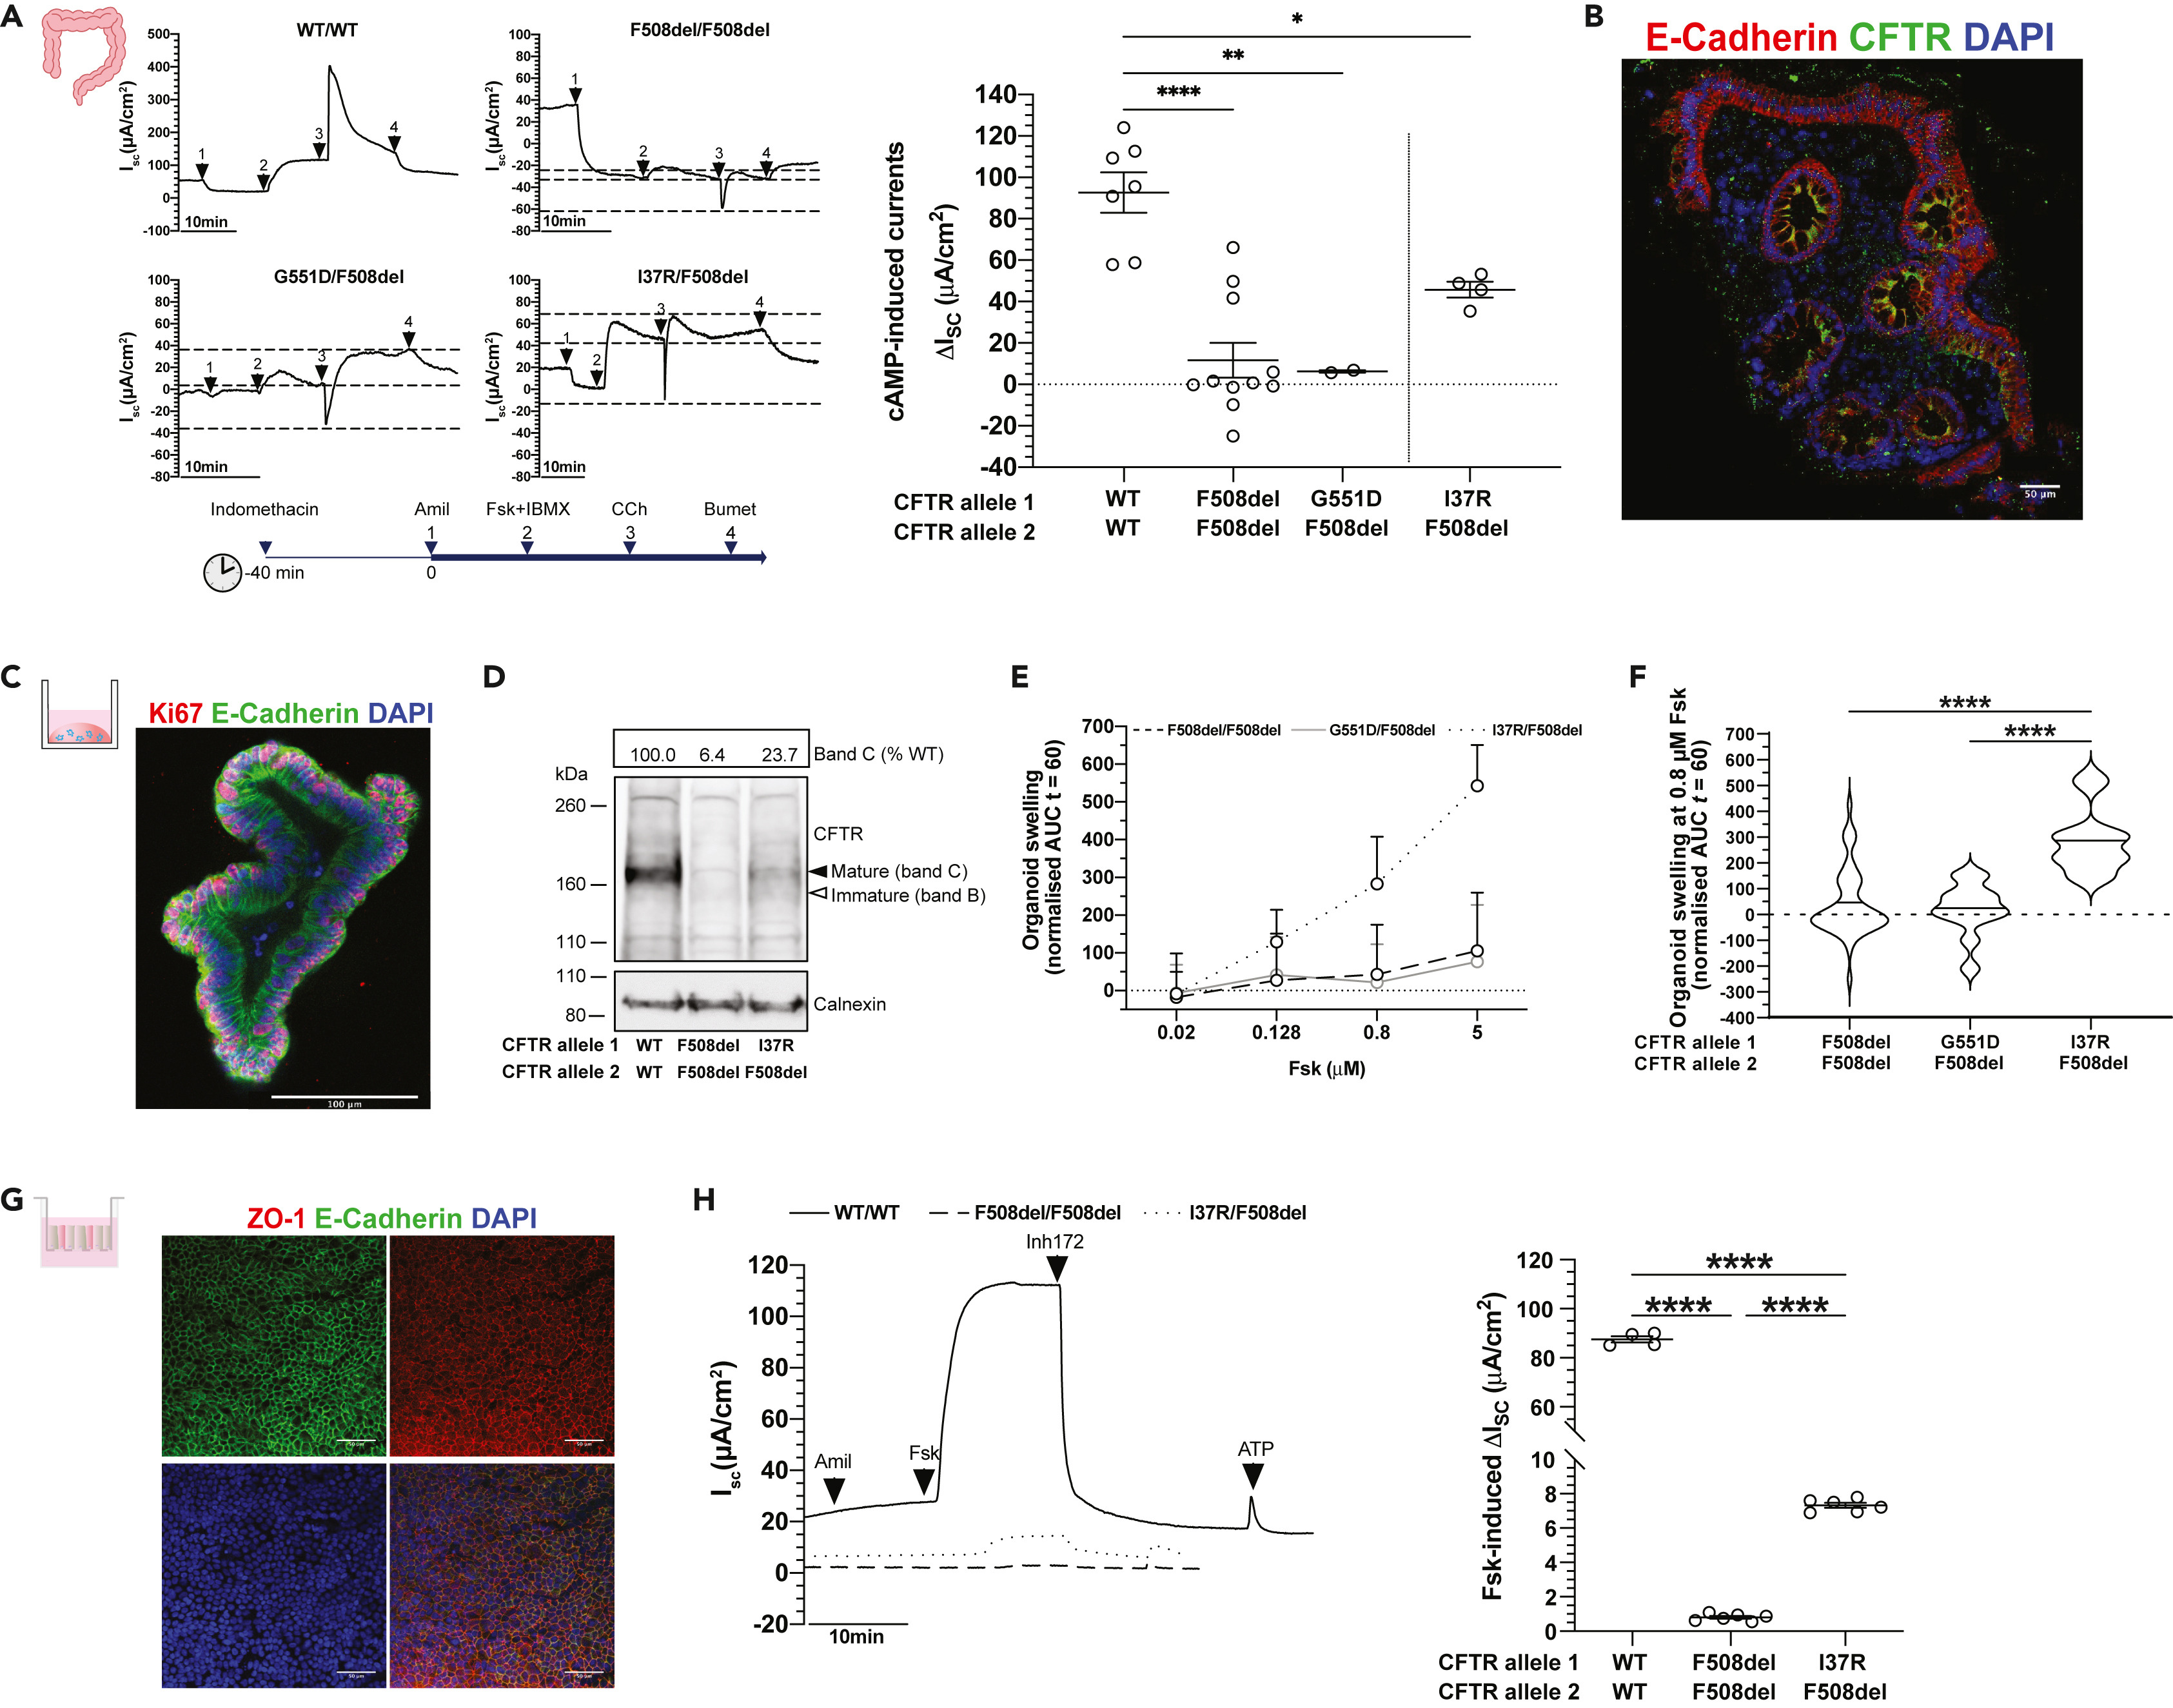
\includegraphics[width=\textwidth]{figures/I37R/rectal_organoids.jpg}
\label{I37R_figure1}
\end{center}
%\captionsetup{singlelinecheck = false, justification=raggedright}
\begingroup
\captionof{figure}[Characterization of I37R-CFTR residual function in rectal biopsies and intestinal organoids]{\textbf{Characterization of I37R-CFTR residual function in rectal biopsies and intestinal organoids}}{
(A) Representative Ussing chamber recordings of intestinal current measurements (ICM) in rectal biopsies from WT-CFTR control participants and participants with CF. Dot plots of cAMP-induced current ($\Delta$Isc-Fsk + IBMX) in participants with WT/WT (n = 2), F508del/F508del (n = 3), G551D/F508del (n = 1), and I37R/F508del (n = 1) CFTR genotypes. Experiments were performed in the presence of 10 $\mu$M indomethacin. Arrows indicate the addition of compounds: 100 $\mu$M apical amiloride (1. Amil), apical and basal addition of 10 $\mu$M forskolin +100 $\mu$M IBMX cocktail (2.Fsk + IBMX), 100 $\mu$M basal carbachol (3.CCh), and 100 $\mu$M basal bumetanide (4.Bumet). The Isc at the time CCh was added (middle horizontal dotted line), and the maximum (top dotted lines) and minimum (bottom dotted lines) Isc induced are indicated. Each dot represents an individual replicate.\\

(B) Immunofluorescence staining of CFTR (green), e-cadherin (red), and DAPI (blue) in a rectal biopsy derived from an I37R/F508del participant. 63x/1.4 oil immersion objective. Scale bar = 50 $\mu$m.\\

(C) Immunofluorescence staining of e-cadherin (green), Ki67 (red), and DAPI (blue) in intestinal organoids derived from an I37R/F508del participant. 20x/0.75 dry objective. Scale bar = 100 $\mu$m.\\

(D) Western blot in WT/WT, F508del/F508del, and I37R/F508del intestinal organoids. CFTR maturation was calculated by measuring the level of mature mutant CFTR (Band C) as a percentage of mature CFTR from WT organoids (\% normal CFTR). All data were normalized to the calnexin loading control. B and C represents the mature, complex-glycosylated CFTR. B and B represents the immature, core-glycosylated CFTR. See Figure S9 for uncropped Western blot images.\\

(E and F) Forskolin-induced swelling (FIS) assay in organoids from participants with F508del/F508del (n = 5), G551D/F508del (n = 2), and I37R/F508del (n = 1) CFTR genotypes. Organoids were stimulated with forskolin (fsk) concentrations ranging from 0.02 to 5 $\mu$M.(E) FIS expressed as the means ± standard deviation (SD) of the area under the curve (AUC) calculated from t = 0 (baseline) to t = 60.(F) FIS of organoids at 0.8$\mu$M fsk at baseline represent residual CFTR function. Data represented as violin plots with mean to show distribution.\\

(G) Immunofluorescence staining of e-cadherin (green), ZO-1 (red), and DAPI (blue) in organoid-derived monolayers from a CF participant. 20x/0.75 dry objective. Scale bars = 50 $\mu$m.\\

(H) Representative Ussing chamber recordings of short circuit current in organoid-derived monolayers from a WT-CFTR control participant and participants with CF. Dot plots of fsk-induced current ($\Delta$Isc-Fsk) in participants with WT/WT (n = 1), F508del/F508del (n = 1), and I37R/F508del (n = 1) CFTR genotypes. Experiments were performed in the presence of 10 $\mu$M indomethacin. Arrows indicate the addition of compounds: 100 $\mu$M apical amiloride, 5 $\mu$M basal fsk, 30 $\mu$M apical CFTR inhibitor CFTRinh-172, and 100 $\mu$M apical ATP. Each dot represents an individual replicate. Data in (A) and (H) represented as mean ± standard error of the mean (SEM). One-way analysis of variance (ANOVA) was used to determine statistical differences. * p $<$ 0.05, ** p $<$ 0.01, **** p $<$ 0.0001.\\
}
\endgroup

\smallskip

Co-activation with carbachol (CCh) resulted in a biphasic response in the I37R/F508del biopsies, characteristic of residual CFTR chloride channel function in the CF colon \cite{graeber2015,veeze1994}. The initial negative Isc peak indicates apical potassium secretion reached 9.4 ± 2.5 $\mu$A/cm$^2$. Following this, the CCh-induced positive Isc indicates the increase of apical chloride secretion reached 15.78 ± 2.07 $\mu$A/cm$^2$. This biphasic response was similarly observed in the G551D/F508del biopsies (25.77 ± 2.16 $\mu$A/cm$^2$) but was diminished in the F508del/F508del biopsies (−2.28 ± 1.65 $\mu$A/cm$^2$). These findings are in accordance with the localization of CFTR protein at the plasma membrane (mature complex-glycosylated CFTR) of the I37R/F508del rectal biopsies, as demonstrated by immunofluorescence staining (green; Figure 1B).

Next, CFTR protein expression and maturation was assessed in I37R/F508del, reference F508del/F508del, and WT/WT organoids using Western blot (Figures 1C and 1D). The expression of complex-glycosylated C band in I37R/F508del organoids was 23.7\% that of the WT/WT organoids, considerably higher than the 6.4\% detected from F508del/F508del organoids (Figure 1D). CFTR activity was then evaluated in I37R/F508del and CF reference intestinal organoids using a fsk-induced swelling (FIS) assay at four fsk concentrations between 0.02 and 5 $\mu$M (Figure 1E). FIS of I37R/F508del intestinal organoids at 0.8 $\mu$M fsk—the optimal concentration for baseline assessment of CFTR activity \cite{dekkers2016}—was 282.9 ± 36.0 (Figures 1E and 1F). This exceeded the baseline FIS of the reference intestinal organoids by at least 7-fold (F508del/F508del: AUC = 42.8 ± 19.4; G551D/F508del: AUC = 21.3 ± 29.4).

The morphological difference between WT (pre-swollen) and CF organoids \cite{cuyx2021}, means comparing CFTR activity between CF and healthy CFTR function by FIS assay cannot be achieved \cite{dekkers2016,vanmourik2019}. In order to compare I37R/F508del to wild-type CFTR activity, organoid-derived monolayers were created (Figure 1G) and CFTR ion transport was performed \cite{zomer-vanommen2018}. Fsk-stimulated CFTR-dependent currents were 9-fold higher in I37R/F508del monolayers than those of reference F508del/F508del monolayers (7.3 ± 0.2 vs 0.8 ± 0.1 $\mu$A/cm$^2$; p $<$ 0.0001), but 12-fold lower than WT/WT monolayers (87.5 ± 1.3 $\mu$A/cm$^2$; p $<$ 0.0001) (Figure 1H). This is consistent with the FIS assay results demonstrating high baseline CFTR activity in I37R/F508del intestinal organoids.

\subsection{I37R-CFTR Functional Response to CFTR Modulator Monotherapy in Intestinal Organoids}

We investigated the functional response of I37R/F508del organoids to single potentiators: VX-770, GLPG1837 (G1837), and genistein (Gen). Treatment with VX-770 minimally increased FIS of I37R/F508del organoids by AUC of 59.7 above baseline at 0.128 $\mu$M fsk (Figures 2A–2C and S1)—the optimal concentration for in vitro assessment of CFTR modulator response to predict clinical effect \cite{dekkers2016}. G1837 and Gen both significantly increased FIS, albeit with different efficacies (655.8 and 256.8, respectively; Figures 2A–2C and S1). None of the potentiator treatments increased FIS in F508del/F508del organoids, indicating no improvement in CFTR activity in response to potentiator therapy (Figure 2C). Only G1837 significantly increased FIS in the G551D/F508del organoids (210.4 ± 57.5; p $<$ 0.01). In comparison to G551D/F508del organoids, G1837 was 3-fold more efficacious in the I37R/F508del organoids (p $<$ 0.0001).


testing


\begin{center}
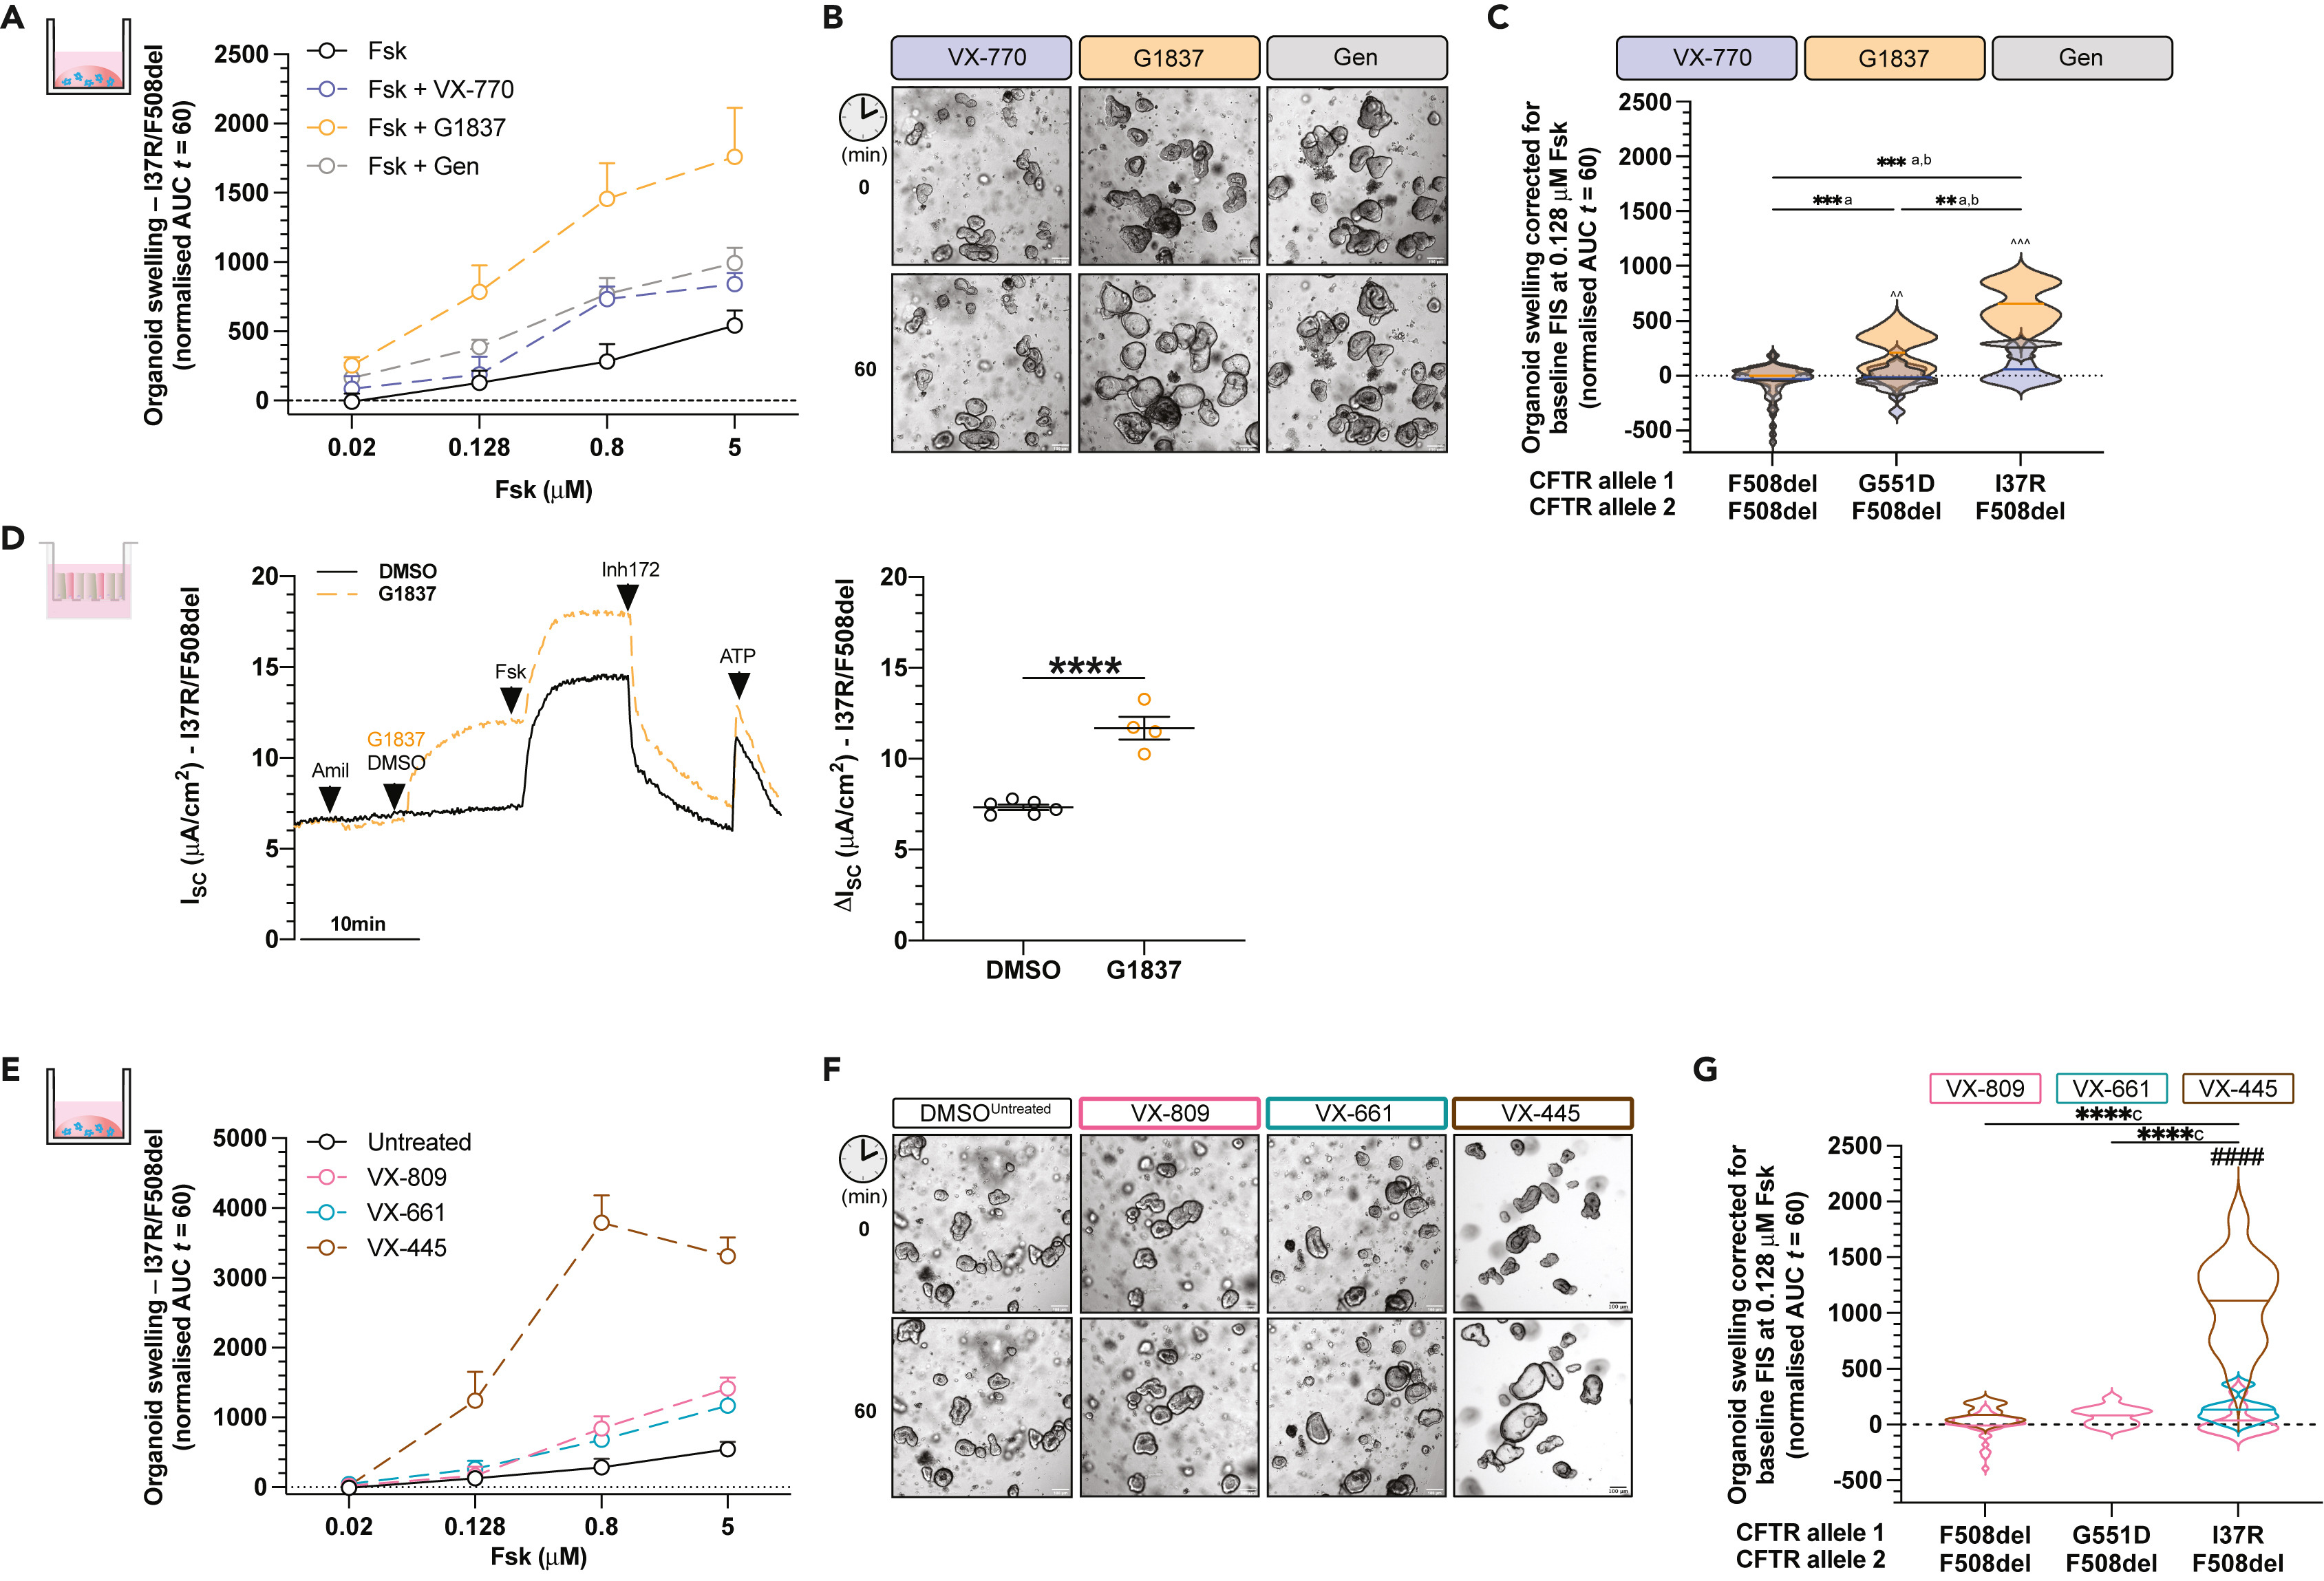
\includegraphics[width=\textwidth]{figures/I37R/rectal_organoids_response.jpg}
\label{I37R_figure2}
\end{center}
\begingroup
\captionof{figure}[Characterization of I37R-CFTR functional response to corrector or potentiator monotherapy in intestinal organoids]{\textbf{Characterization of I37R-CFTR functional response to corrector or potentiator monotherapy in intestinal organoids}}{
Forskolin-induced swelling (FIS) assay in organoids from participants with F508del/F508del (n = 5), G551D/F508del (n = 2), and I37R/F508del (n = 1) CFTR genotypes. Organoids were incubated overnight with 0.03\% DMSO (untreated) or 3 $\mu$M VX-809 or 3 $\mu$M VX-661 or 3 $\mu$M VX-445. After 24 h, organoids were stimulated with fsk concentrations ranging from 0.02 to 5 $\mu$M, either alone or in combination with potentiator monotherapy (3 $\mu$M VX-770 or 3 $\mu$M G1837 or 50 $\mu$M Gen).\\

(A) FIS of I37R/F508del organoids stimulated with VX-770, GLPG1837 (G1837), or genistein (Gen) monotherapy, expressed as the means ± standard deviation (SD) of the area under the curve (AUC) calculated from t = 0 (baseline) to t = 60 min.\\

(B) Representative brightfield images of I37R/F508del organoids at baseline (t = 0) and after 1 h of stimulation (t = 60) at 0.128 $\mu$M fsk. Scale bars = 100 $\mu$m.\\

(C) FIS of organoids at 0.128$\mu$M fsk following stimulation with VX-770, GLPG1837 (G1837), or genistein (Gen) monotherapy. Data corrected for baseline FIS and represented as violin plots with mean to show distribution.\\

(D) Representative Ussing chamber recordings of short circuit current in I37R/F508del organoid-derived monolayers. Dot plots of total currents stimulated by DMSO or G1837 plus fsk. Experiments were performed in the presence of 10 M indomethacin. Arrows indicate the addition of compounds: 100 M apical amiloride, apical addition of either vehicle control 0.01\% DMSO or 10 $\mu$M G1837, 5 $\mu$M basal fsk, 30 $\mu$M apical CFTR inhibitor CFTRinh-172, and 100 $\mu$M apical ATP. Each dot represents an individual replicate. Data represented as mean ± standard error of the mean (SEM).\\

(E) FIS of I37R/F508del organoids pre-incubated with corrector (VX-809 or VX-661 or VX-445) for 24 h, expressed as the means ± standard deviation (SD) of the area under the curve (AUC) calculated from t = 0 (baseline) to t = 60 min.\\

(F) Representative brightfield images of I37R/F508del organoids at baseline (t = 0) and after 1 h of stimulation (t = 60) at 0.128 $\mu$M fsk. Scale bars = 100 $\mu$m.\\

(G) FIS of organoids at 0.128$\mu$M fsk following incubation with corrector (VX-809 or VX-661 or VX-445) for 24 h. Data corrected for baseline FIS and represented as violin plots with mean to show distribution. One-way analysis of variance (ANOVA) was used to determine statistical differences except in (D) where unpaired t test was used. **p $<$ 0.01, ***p $<$ 0.001, and ****p $<$ 0.0001. aP for G1837, bP for Gen and cP for VX-445 of I37R/F508del, \^P for G1837 vs VX-770, or Gen and \#P for VX-445 vs VX-809 or VX-661.\\
}
\endgroup

Because G1837 demonstrated the greatest restoration of CFTR activity in I37R/F508del organoids, we evaluated G1837 treatment of I37R/F508del organoid-derived monolayers. G1837 led to a significant 1.5-fold increase in fsk-stimulated currents ($\Delta$Isc: 4.4 $\mu$A/cm$^2$; p $<$ 0.0001) (Figure 2D). This is consistent with the FIS of I37R/F508del organoids, indicating that I37R-CFTR responds to potentiator agents.

Given the I37R/F508del high residual CFTR activity and its localization at the epithelial cell surface, we hypothesized that the I37R-CFTR mutation has minimal impact on CFTR protein folding or maturation. Treatment of I37R/F508del organoids with type I corrector agents (VX-809 or VX-661) did not significantly increase FIS above baseline (Figures 2E–2G and S1). In contrast, treatment of I37R/F508del organoids with a type III corrector agent (VX-445) significantly increased FIS by AUC of 1112.5 above baseline, greater than those in the F508del/F508del organoids (42.5). VX-445 has been shown to act as both a corrector and potentiator for certain CFTR mutations \cite{laselva2021,shaughnessy2021,veit2021}. Acute treatment of I37R/F508del organoids with VX-445 did not improve potentiation of CFTR (Figure S1). This supports the observation that VX-445-stimulated rescue of CFTR in I37R/F508del organoids acts by a correction mechanism improving I37R mild folding and processing defects. I37R-CFTR functional response to CFTR modulator co-therapies in intestinal organoids.

Combination treatments of CFTR modulators are used to treat patients bearing CFTR mutations with multiple functional defects such as F508del and patients who are heterozygous for CFTR mutations. We investigated the effect of combinations of potentiators. Dual potentiator combinations increased FIS of I37R/F508del organoids to a greater extent than the respective single potentiators (Figure 3A) and had a synergistic effect, where the FIS was greater than the sum of the respective single potentiators (Table S4). Despite G1837 + Gen having greater efficacy than the other dual potentiator combinations, the magnitude of response was not statistically different between the different combinations of dual potentiators (Figure 3A).

Co-therapy with a corrector (VX-809 or VX-661) and dual potentiators significantly (p $<$ 0.01) increased FIS of I37R/F508del organoids compared to co-therapy of a corrector with VX-770 or Gen, but not G1837 (Figure 3B). VX-809/G1837 + Gen co-therapy had the greatest efficacy, increasing FIS 1904.0 above baseline. In contrast, corrector/VX-770 + Gen co-therapy had the least efficacy. This trend was consistent with that of the dual potentiators synergistic effect.

Dual correctors (VX-445+VX-661) increased FIS in I37R/F508del organoids by AUC of 1856.6 above baseline, which corresponds with the level of rescue achieved by the most effective corrector/dual potentiator co-therapy (VX-809/G1837 + Gen). The triple combination therapy with dual correctors and a potentiator further increased FIS in I37R/F508del organoids by AUC of 3101.6 above baseline. It is therefore the most effective modulator combination tested in this study.

\begin{center}
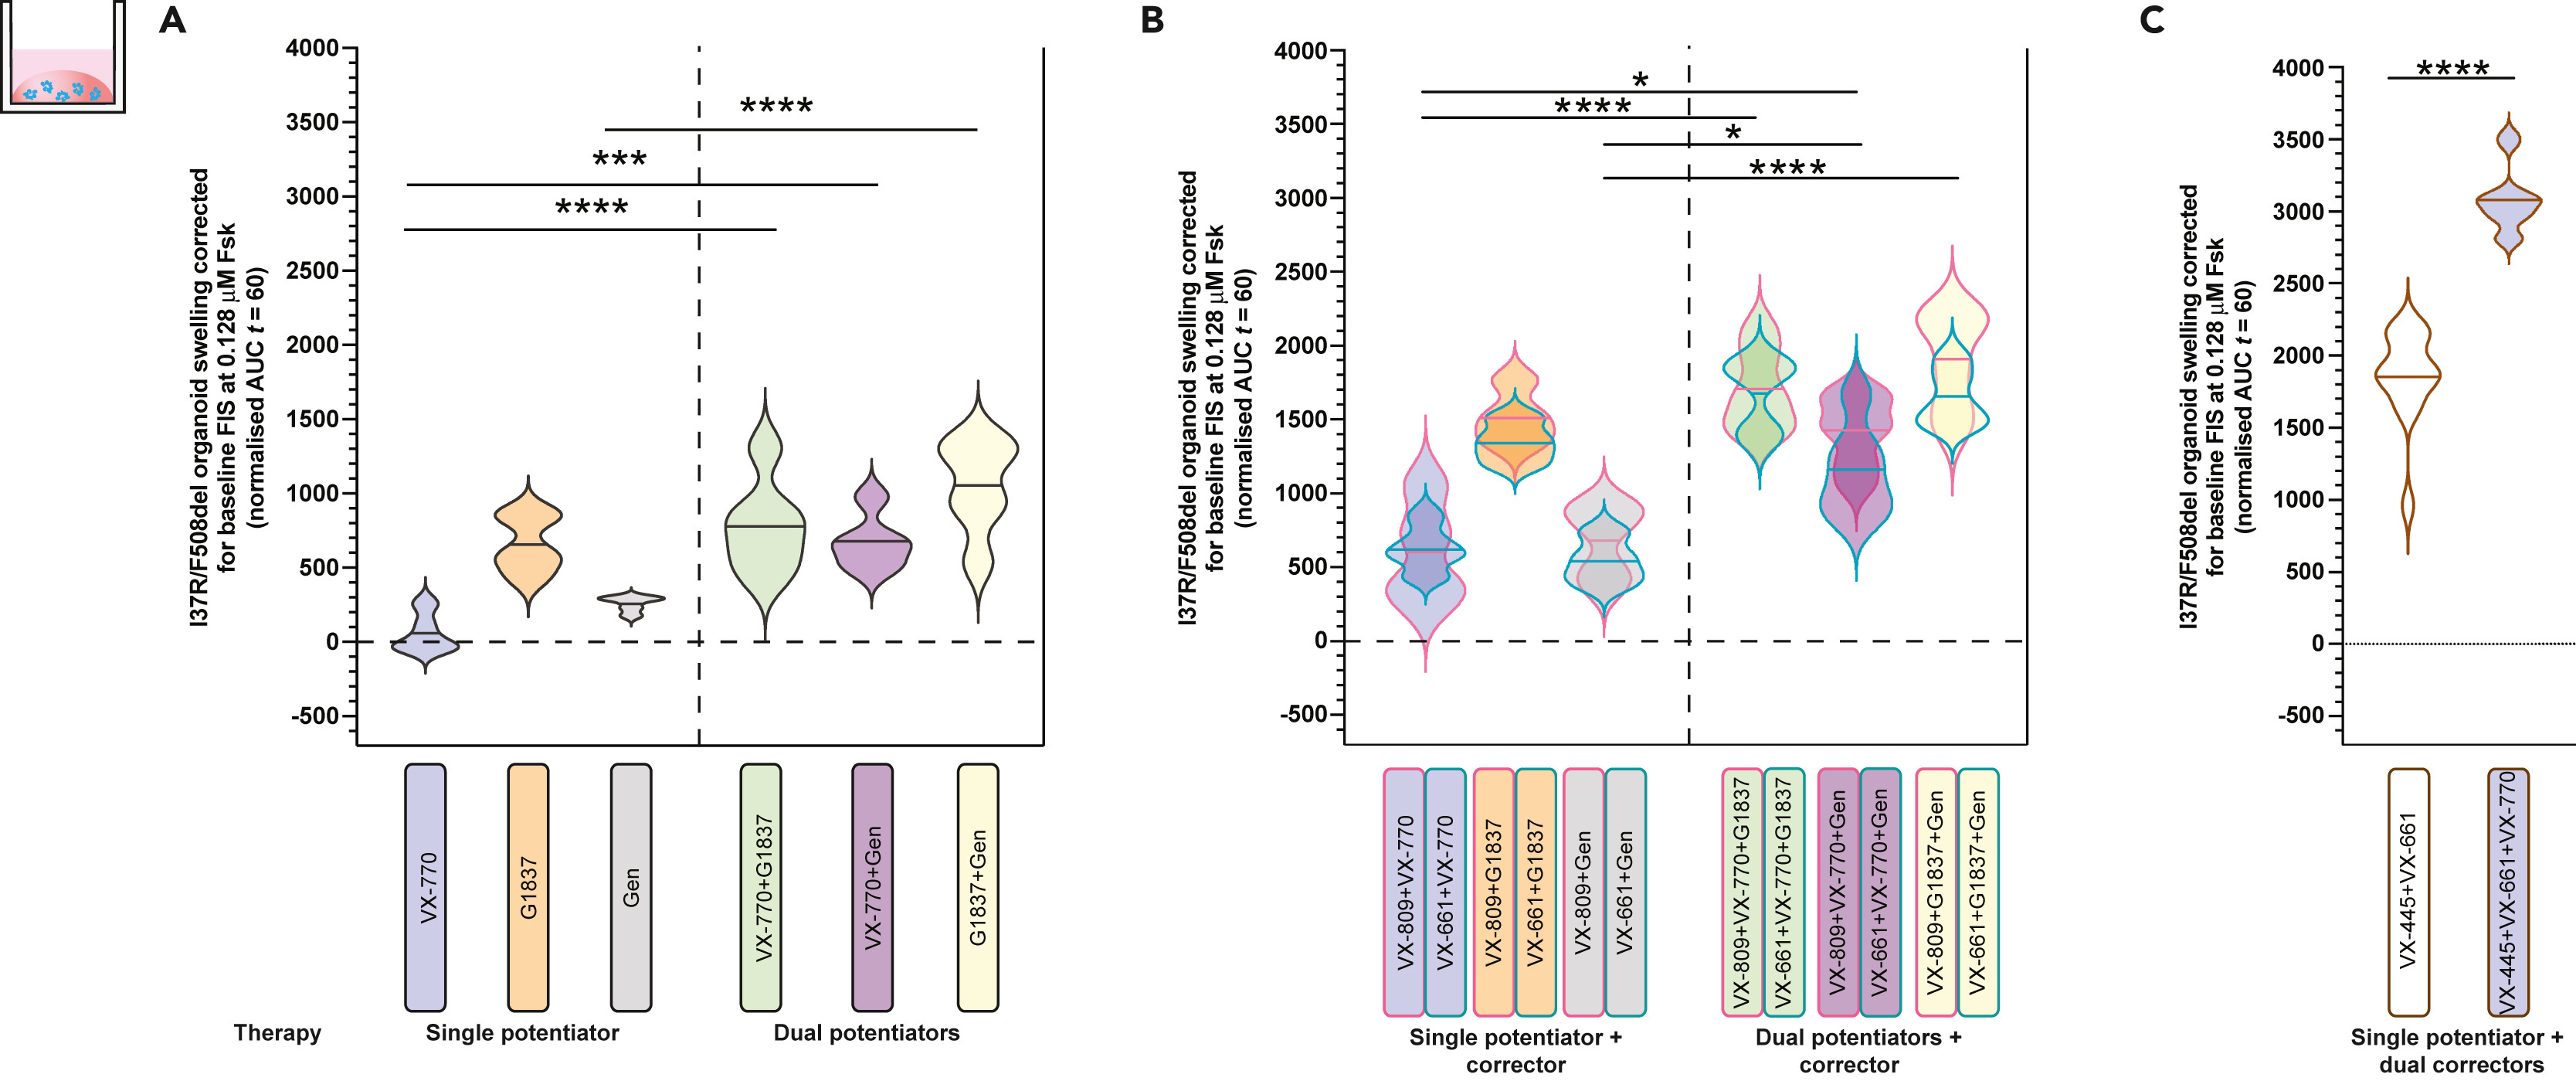
\includegraphics[width=\textwidth]{figures/I37R/rectal_organoids_triple_therapy.jpg}
\label{I37R_figure3}
\end{center}
\begingroup
\captionof{figure}[Characterization of I37R-CFTR functional response to dual potentiator or corrector therapy or corrector(s)-potentiator(s) co-therapy in intestinal organoids]{\textbf{Characterization of I37R-CFTR functional response to dual potentiator or corrector therapy or corrector(s)-potentiator(s) co-therapy in intestinal organoids}}{
	Forskolin-induced swelling (FIS) assay in organoids from participants with F508del/F508del (n = 5), G551D/F508del (n = 2), and I37R/F508del (n = 1) CFTR genotypes.\\

	(A and B) Organoids were incubated overnight with 0.03\% DMSO (untreated) or 3 $\mu$M VX-809 or 3 $\mu$M VX-661 or 3 $\mu$M VX-445 + 18 $\mu$M VX-661. After 24 h, organoids were stimulated with fsk ranging in concentration from 0.02 to 5 $\mu$M, either alone or in combination with a single potentiator (3 $\mu$M VX-770 or 3 $\mu$M G1837 or 50 $\mu$M Gen) or dual potentiators (VX-770 + G1837 or VX-770 + Gen or G1837 + Gen). FIS of organoids at 0.128$\mu$M fsk stimulated with VX-770, GLPG1837 (G1837), or genistein (Gen) or their combinations, following (A) 24 h pre-incubation with DMSO (untreated) or (B) corrector (VX-809 or VX-661), respectively.\\

	(C) FIS of organoids at 0.128$\mu$M fsk stimulated without or with VX-770, following 24 h pre-incubation with dual correctors (VX-445+VX-661). Data corrected for baseline FIS and represented as violin plots with mean to show distribution. One-way analysis of variance (ANOVA) was used to determine statistical differences except in (C) where unpaired t test was used. *p $<$ 0.05, ***p $<$ 0.001, ****p $<$ 0.0001
}
\endgroup

\subsection{I37R-CFTR Perturbs the Noose Structure of the Lasso Motif}

We next characterized the structural defect of I37R-CFTR using MD simulations. The primary structure of the lasso motif (M1-L69) is conserved across 230 vertebrate species (Figure S2, Table S5). The lasso motif formed a noose structure that rested against TMD2 (Figure 4A). Amino acids V12-R29 were embedded in the plasma membrane while the rest of the lasso motif resided in the cytosol. The noose structure was maintained by a salt bridge formed between K26 and D36 (Figure 4B). I37 was positioned in the center of this noose, within a hydrophobic pocket formed by amino acids from the lasso, TMD2, and the poorly resolved R domain in the cytosol (Figure 4C).

\begin{center}
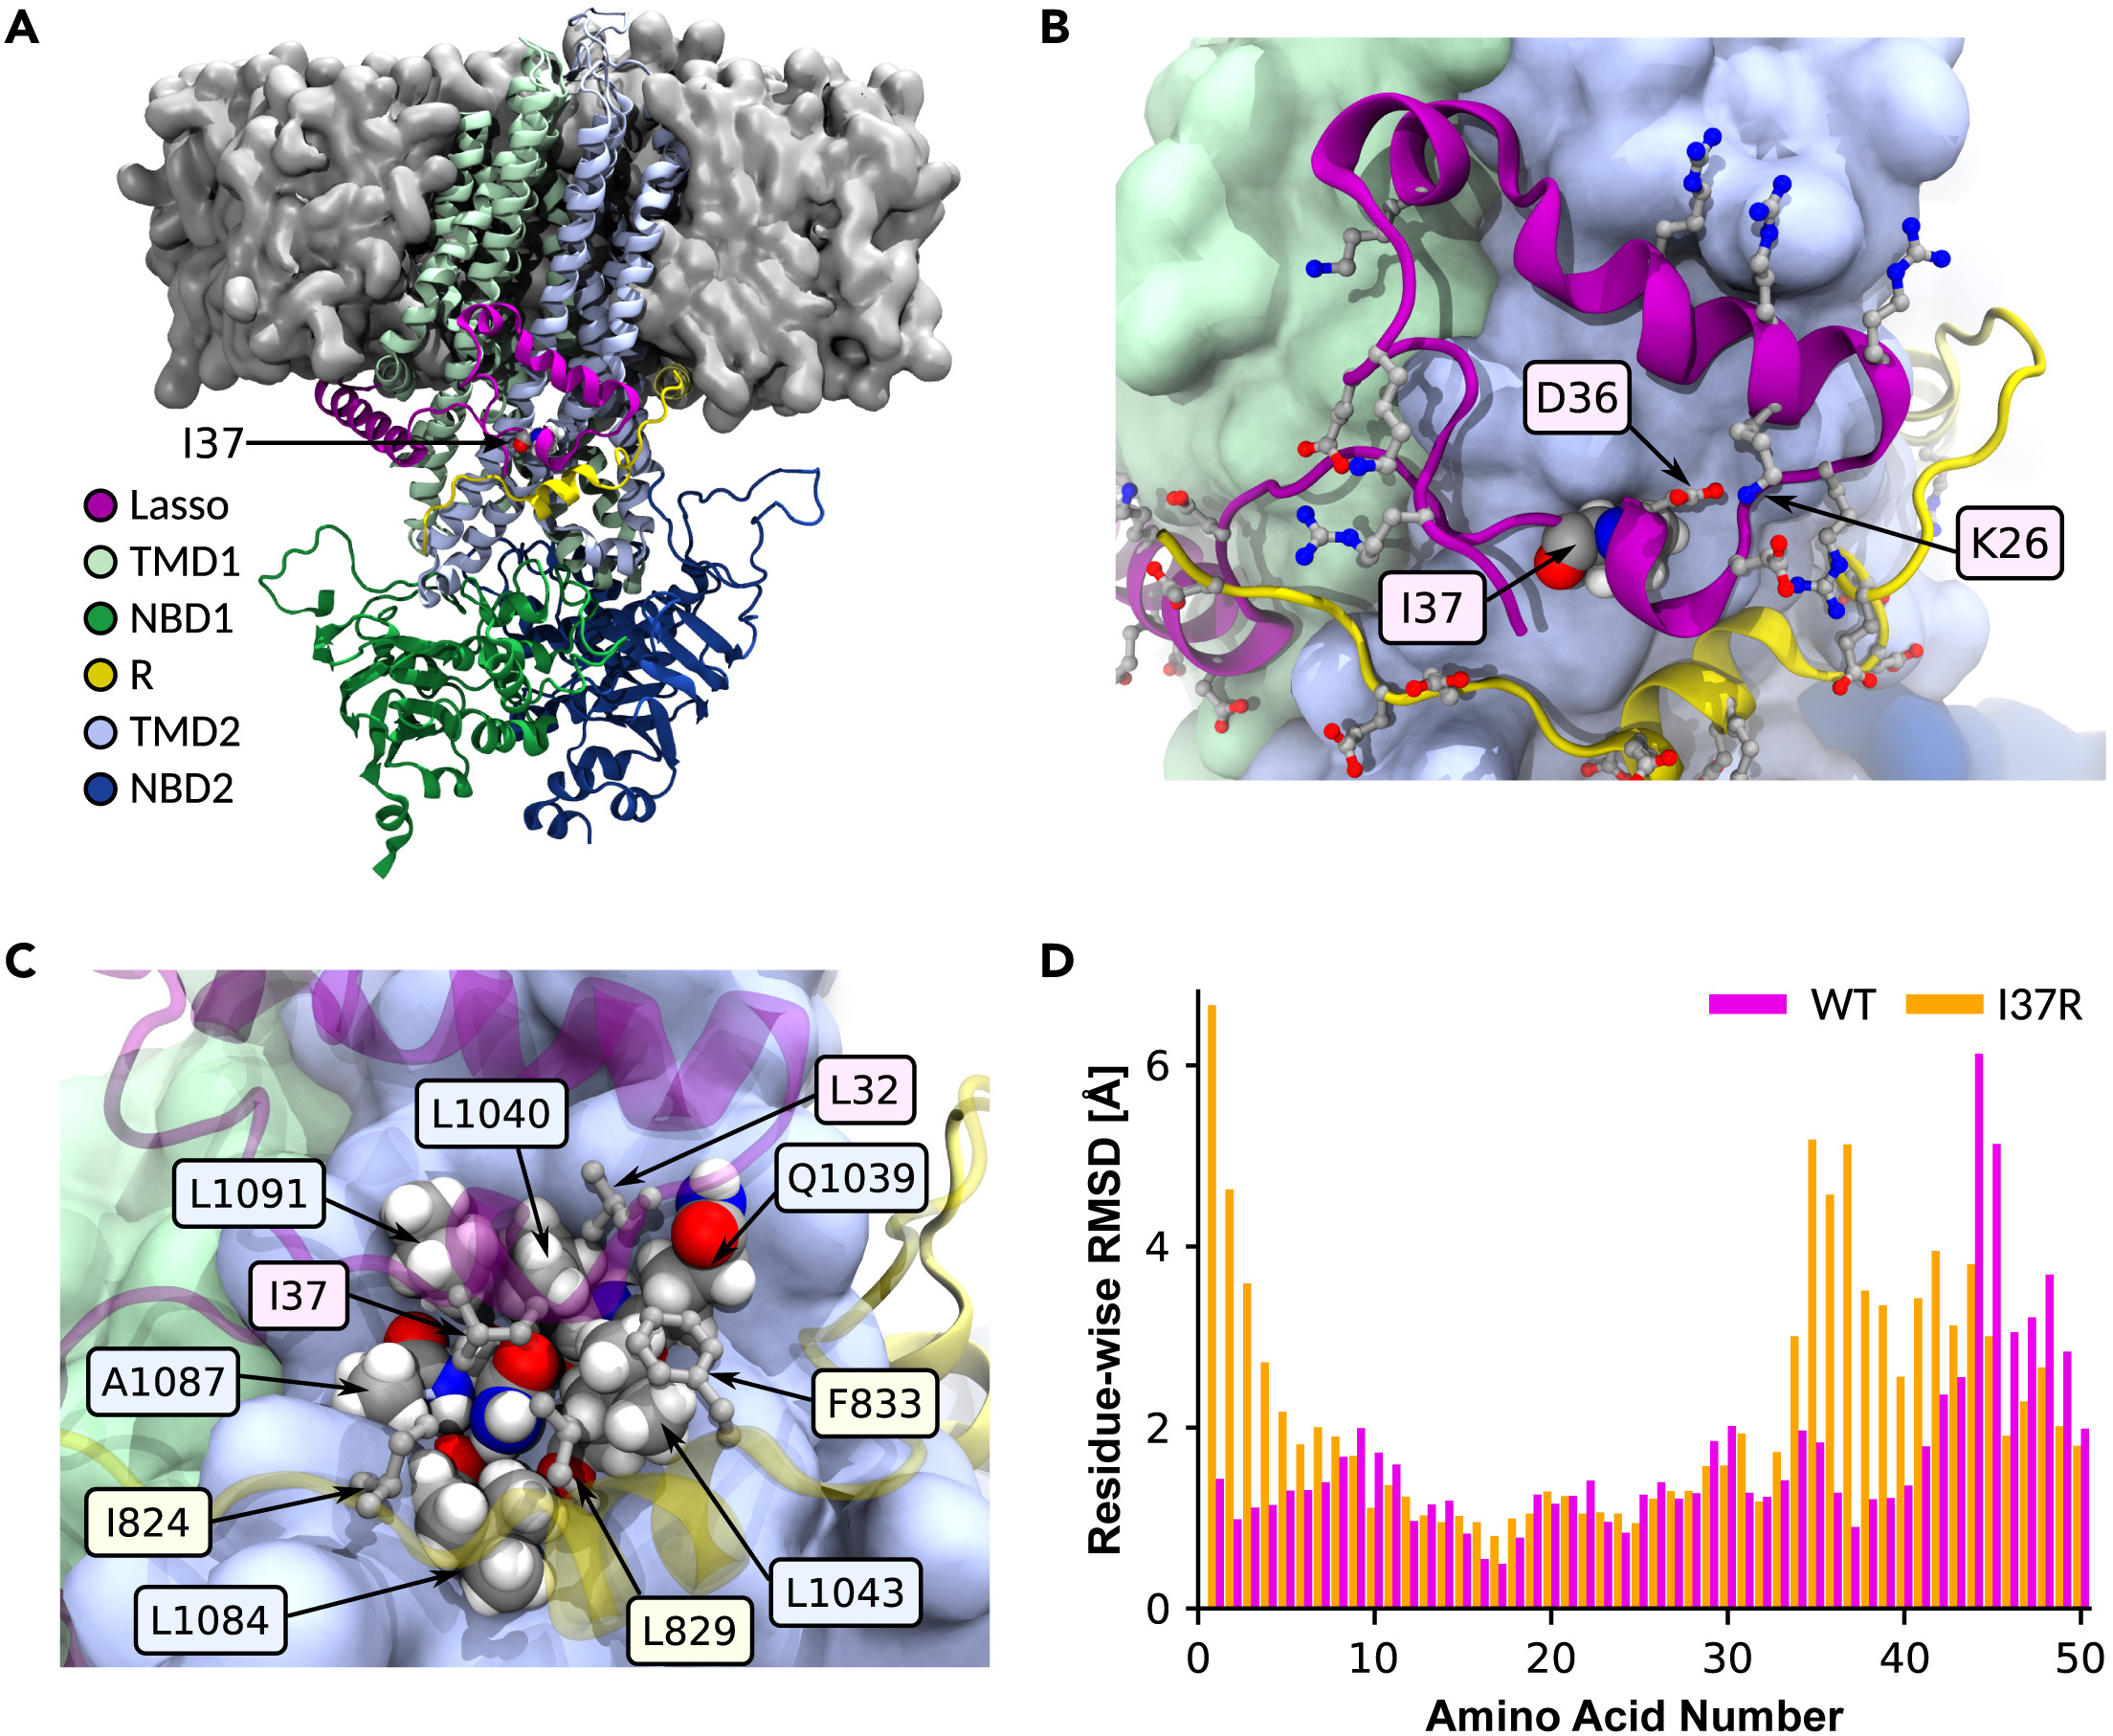
\includegraphics[width=\textwidth]{figures/I37R/MD_cftr.jpg}
\label{I37R_figure3}
\end{center}
\begingroup
\captionof{figure}[Placement of I37R within the lasso motif and the resulting changes to its conformation]{\textbf{Placement of I37R within the lasso motif and the resulting changes to its conformation}}{
	(A) Ribbon structure of human CFTR, partially embedded within the plasma membrane (gray surface). I37 rendered as spheres. TMD: transmembrane domain; NBD: nucleotide-binding domain; R: regulatory domain (R domain).\\

	(B) K26-D36 salt bridge stabilizing the noose structure of the lasso motif. Charged amino acids depicted as balls and sticks. I37 rendered as spheres, and color-coded by element (gray: C; white: H; red: O; blue: N).\\

	(C) I37 positioned within a hydrophobic pocket formed by amino acids from the lasso motif, TMD2, and poorly resolved R domain. Relevant amino acids labeled and depicted as spheres in TMD2, and as balls and sticks in lasso motif and R domain.\\

	(D) Residue-wise root-mean-square deviation (RMSD) to the C-alpha atoms of the WT-CFTR 6MSM model, measuring the conformational change of the WT (pink) and I37R mutant (orange) lasso after 2 $\mu$s simulations. Values are means sampled over the last $\mu$s of simulations.\\
}
\endgroup

Mutation of the evolutionarily conserved, non-polar and uncharged isoleucine (I) of I37 to a positively charged arginine (R) introduced an unstable lone charge into the hydrophobic pocket within the lasso motif noose. We hypothesized that this likely results in the rotation of the R37 side chain out of the hydrophobic pocket, and possible coordination with negative charges in the nearby R domain.

To identify a reasonable conformation of the mutant lasso motif, the WT 6MSM model was mutated to R37 and three 2 $\mu$s simulations were performed at physiological temperature (310 K). The R37 side chain rotated out of the hydrophobic pocket in only one of the three simulations. The difference between the root-mean-square deviation (RMSD) of the noose structure of I37R-CFTR compared to the WT was on average 2.8 $\mbox{\AA}$ at the amino acids M1-L6, and 1.8 $\mbox{\AA}$ at L34-S50 (Figure 4D). To confirm this observation, repeat simulations were performed at 350 K (40$^\circ$C above physiological temperature), a temperature shown to accelerate the potential conformational transitions of proteins \cite{beckerman2015}. In these higher temperature simulations, the root-mean-square fluctuation (RMSF) of the region around amino acid 37 doubled in two out of three simulations, compared to WT-CFTR at 310K (Figure S3). This confirmed the destabilization of the lasso motif by I37R-CFTR. All WT-CFTR domains and the surrounding bilayer remained stable at the elevated temperature (Figures S4 and S5).

\subsection{I37R Mutation Strengthens Lasso Motif Interaction with the R-domain}

In the 6MSM structure, the R domain is largely unresolved with two exceptions: the first (Q637) and last (T845) amino acids that adjoin neighboring domains, and the backbone atoms of a 17 amino acid segment. This latter segment consists of an eight amino acid disordered coil followed by a nine amino acid alpha-helix \cite{zhang2018a}. The alpha-helix was separated by approximately 10$\mbox{\AA}$ (1 nm) minimum C-alpha distance to I37 in the lasso motif. This suggested a likely interaction between this segment of the R domain and I37, which necessitated partial modeling of the R domain (Figure 5A).

\begin{center}
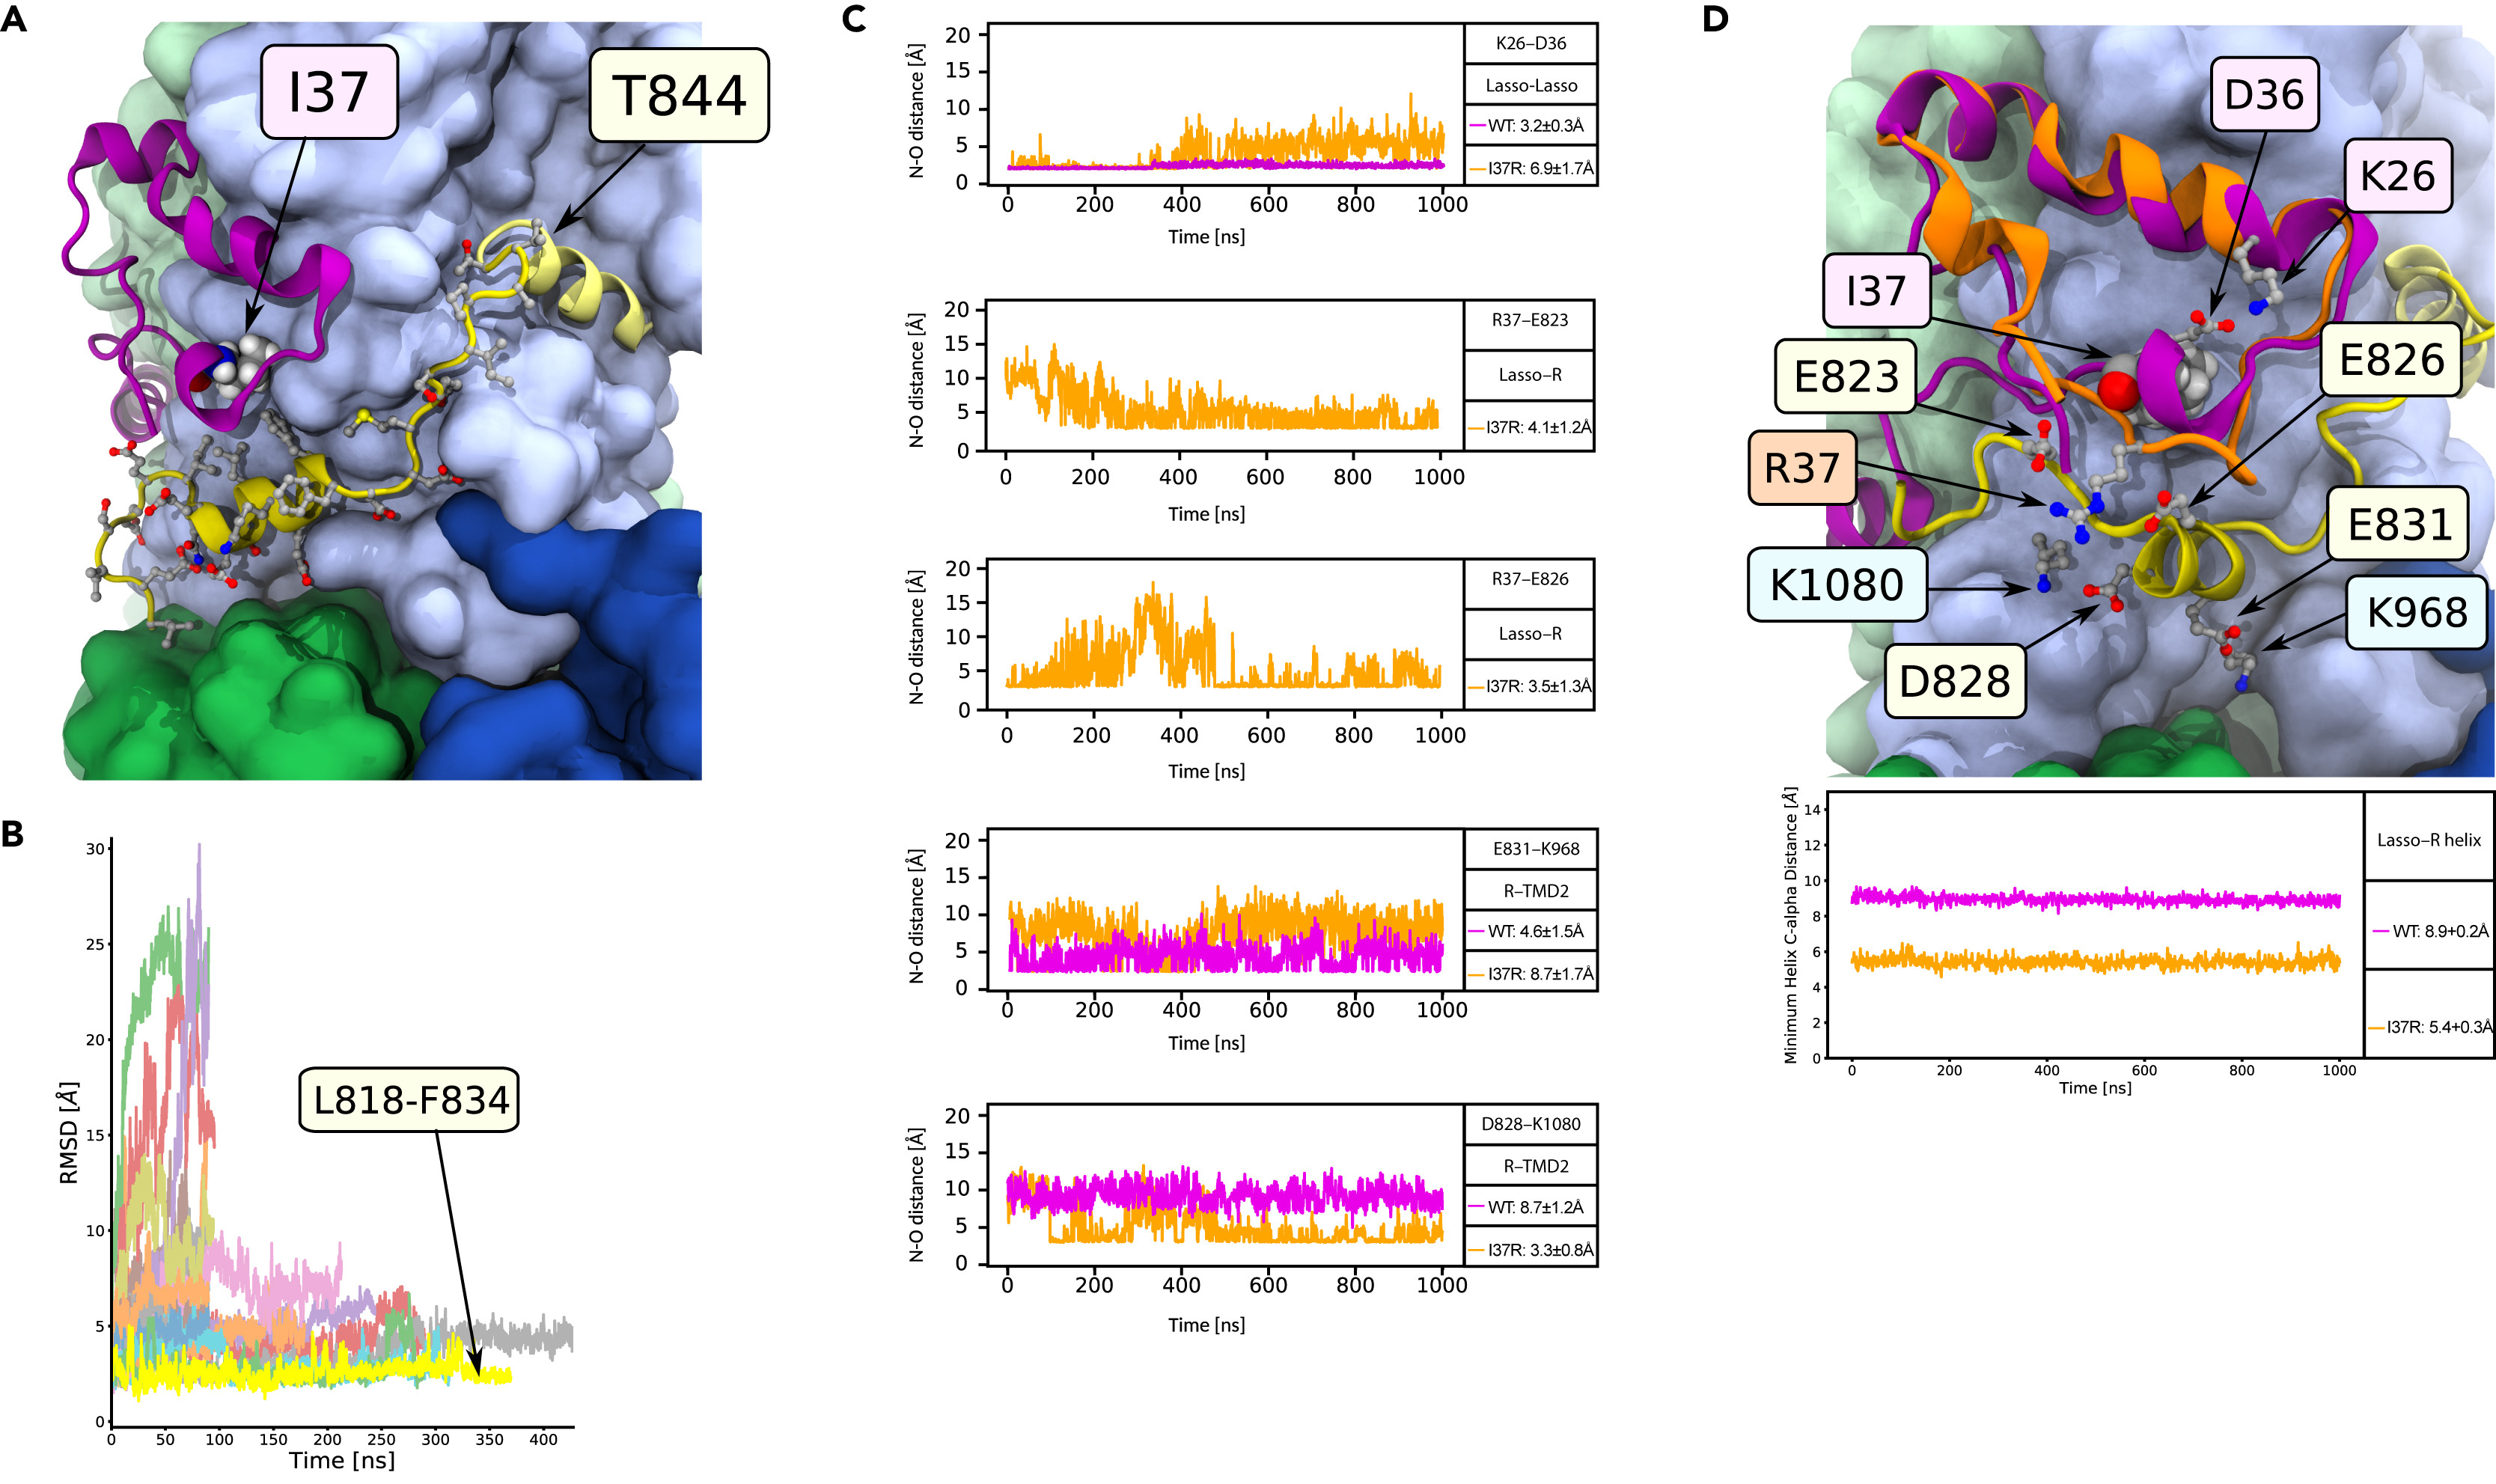
\includegraphics[width=\textwidth]{figures/I37R/MD_cftr_2.jpg}
\label{I37R_figure3}
\end{center}
\begingroup
\captionof{figure}[I37R interacts with a previously unresolved section of the R domain]{\textbf{I37R interacts with a previously unresolved section of the R domain}}{
	(A) The reconstructed R domain amino acids (yellow), depicting the assignment of L818-F834 to the 17 amino acids with only the backbone resolved in the 6MSM structure, and the linking residues to T845 in TMD2. Lasso motif in purple. Side chains depicted as balls and sticks.\\

	(B) The stabilities of all 24 modeled R domain assignments, quantified by RMSD to the 6MSM structure. The most stable alignment of the 17 unidentified amino acids, L818-F834, is highlighted yellow. The full list of tested assignments is shown in Supplementary material 9.\\

	(C) The minimum N-O distance between newly formed and disrupted salt bridges in the I37R mutant. Distance less than 4 Å indicates direct contact. Values are means ± standard deviations (SD), sampled over the last 500 ns of simulations.\\

	(D) Conformational changes in the I37R mutant (orange) compared to WT (purple) lasso motif, which brings it closer to the R domain (yellow). Minimum C-alpha atom distance between amino acid 37 and the R domain helix (E826-F834) in I37R and WT.
}

\endgroup

Modeling of these 17 unidentified amino acids was performed by creating 24 different in silico models of this segment based on the 6MSM structure. In each model, a unique 17 amino acid sequence was determined with a sliding window of one amino acid, starting backwards from amino acid T842 due to the alpha-helix’s 20 $\mbox{\AA}$ proximity to T845. The 17 amino acids were then connected to T845 with the missing linking amino acids. The structural stability of all 24 modeled segments was tested by performing up to 300 ns simulations for each model and comparing the backbone RMSD measurements against 6MSM (Figures 5B and S6). The model with the lowest RMSD (3 $\mbox{\AA}$) and thus the highest stability was attained when L818-F834 was assigned to the unidentified 17 amino acids, of which the alpha-helix maps to E826-F834 (Figures 5B and S6). This assignment was corroborated by NMR measurements of the isolated R domain in solution, where the same segment retained partial helicity \cite{baker2007}. Predictions of the structure of human CFTR by Alphafold2 also aligned with this assignment of primary structure to the unidentified amino acids (Figure S7) \cite{jumper2021}. Several favorable interactions between this R domain model and other parts of the CFTR protein further supported this assignment (Figures 4C and 5D). Two hydrophobic amino acids (L829 and F833) contributed to the hydrophobic pocket that stabilized the lasso motif around I37. The negatively charged E831 formed a salt bridge with positively charged K968 in TMD2. Together, these interactions secured the R domain alpha-helix into position throughout an extended 2 $\mu$s simulation, resulting in a smaller minimum C-alpha distance to the lasso motif of 8.9 ± 0.2 $\mbox{\AA}$ compared to the 10 $\mbox{\AA}$ in the 6MSM cryo-EM structure.

The reoriented R in position 37 in the I37R mutant protein, which pointed out of the hydrophobic pocket, rearranged the salt bridge network supporting the lasso motif by breaking the evolutionarily conserved salt bridge K26–D36. Two new salt bridges were formed, one with the negatively charged E823 and another with E826 of the R domain (Figure 5C). Furthermore, the E831–K968 salt bridge between the R and TMD2 domains in the WT was exchanged for a D828–K1080 salt bridge in I37R-CFTR (Figure 5C). The backbone motions required to accommodate these new charge interactions also perturbed parts of the lasso motif (Figure S3) and R domain. The lasso N-terminus shifted its position towards the R domain and reduced the minimum C-alpha distance between them by 3.5 $\mbox{\AA}$ (Figure 5D). The overall result was a tighter coupling between the lasso and the R domain which is anticipated to inhibit the R domain movements required for channel gating.

\section{Discussion}

We have described the functional and structural defects of I37R, a novel CF-causing mutation in the segment of the CFTR lasso motif which interacts with the R domain. These were compared to reference CFTR mutations which have known functional defects, either a CFTR folding/maturation (F508del/F508del) or a gating (G551D/F508del) defect. First, ICM performed in I37R/F508del rectal biopsies identified I37R confers high residual activity (50\% of WT-CFTR activity). High baseline CFTR activity was similarly observed in FIS of I37R/F508del intestinal organoids and Isc measurements in organoid-derived monolayers. Given we and others showed that F508del is a severe mutation which contributes little functional CFTR \cite{vangoor2011}, this suggests that I37R mutation produces CFTR protein which localizes to the epithelial cell surface. These observations are consistent with the patient's mild CF clinical phenotypes (pancreatic sufficient with faecal elastase $>$ 500 $\mu$g/g, FEV1 z-score -0.11, 99\% predicted).

We also characterized the response of I37R-CFTR to modulators (potentiators and correctors) in I37R/F508del intestinal organoids and organoid-derived monolayers. I37R was responsive to potentiators which improve CFTR gating function and a newly approved corrector (VX-445). Among the three potentiator agents tested, the response to VX-770 was minimal. The reason for the lack of efficacy of VX-770 is not known, because molecular modeling studies propose that VX-770 shares the same mechanism of action and binding sites with G1837 \cite{liu2019, yeh2019}. Both VX-770 and G1837 are proposed to potentiate CFTR by increasing channel open probability (Po) through stabilization of the open-pore conformation, independent of NBD dimerization and ATP hydrolysis which normally controls channel gating \cite{vangoor2009, yeh2017}. However, the differing potentiator efficacies are not a new observation. G1837 was previously shown to be more potent and effective than VX-770 in human bronchial epithelial cells from a G551D/F508del and a R334W/F508del CF participant \cite{gees2018, vanderplas2018}. Similar observations were reported in heterologous HEK293 cells expressing Class III (G551D, G178R, and S549N) and Class IV (R117H) CFTR mutants \cite{gees2018, vanderplas2018}. We conclude that perhaps G1837 has additional binding sites or actions distinct from VX-770, which in the case of I37R-CFTR, results in significant potentiation of the CFTR channel.

We further showed that dual potentiator combinations exerted synergistic restoration of CFTR activity in I37R/F508del organoids. This synergistic restoration is not exclusive to I37R-CFTR, because similar findings have been reported for other CFTR mutations responsive to potentiators \cite{dekkers2016a, phuan2018,phuan2019, veit2020}. Synergism is commonly achieved when potentiators have distinct binding sites and mechanisms of actions. One potentiator could induce allosteric interactions that favor the activity of the other potentiator \cite{nussinov2013}. The potentiator synergy observed in our dual potentiator combinations supports our hypothesis that G1837 may have additional binding sites or mechanisms of action to VX-770. While VX-770 has been shown to provide clinical benefit to patients with responsive mutations \cite{berkers2020, mckone2014, volkova2020}, it does not restore the Po of gating defect mutants (G551D-CFTR) to full WT-CFTR activity \cite{vangoor2009}., 2009). This opens the possibility that using another potentiator with a different mechanism of action could complement VX-770 activity and increase CFTR activity beyond that of VX-770 monotherapy. While VX-770 and G1837 act independently of NBD dimerization and ATP hydrolysis \cite{vangoor2009,yeh2017}, genistein promotes ATP-dependent gating of CFTR by binding to the NBD1/2 interface and inhibiting ATP hydrolysis \cite{sohma2013}. Genistein has been demonstrated to increase VX-770-potentiated CFTR activity in intestinal organoids, even when VX-770 was used at near-saturating concentrations \cite{dekkers2016a}. Our observations reiterate and expand on these findings to suggest that potentiators with different mechanisms of action could provide synergistic restoration of CFTR activity to responsive CFTR mutations compared to potentiator monotherapy.

Chronic treatment with type III corrector VX-445 rescued CFTR activity in I37R/F508del organoids, while neither type I correctors (VX-809 or VX-661) rescued activity. This response is attributed to the I37R and not the F508del mutation in the I37R/F508del organoids, because VX-445 did not restore CFTR activity in F508del/F508del organoids. While VX-445 has been shown to have partial potentiator activity \cite{laselva2021,shaughnessy2021, veit2021}, VX-445 did not potentiate CFTR activity in I37R/F508del organoids when administered acutely. This is the first study to interrogate the potentiator action of VX-445 in intestinal organoids; however, previous studies have been performed in donor-derived bronchial and nasal epithelial cells and immortalized cell lines. The higher correction efficacy of VX-445 when compared with VX-809/VX-661 has previously been shown, although this is likely to be dependent on the CFTR variant \cite{keating2018,veit2020a, veit2021a}. For instance, direct binding of VX-445 to NBD1 to stabilize and prevent the domain unfolding may make it more effective in correcting CFTR mutations that impact NBD1 function (such as F508del located in NBD1).

The lack of I37R-CFTR correction by VX-809 or VX-661 could be attributed to the dependency of these modulators binding to and stabilizing the TMD1. TMD1 function is modulated by interaction with lasso helix 2 (Lh2, aa A46–L61) as deletion of Lh2 from the WT CFTR was shown to completely abrogate VX-809-mediated CFTR maturation \cite{sabusap2021}. MD studies showed that VX-809 occupancy at the TMD1 binding site causes the Lh2 to move, such that the network of salt bridges in Lh2 holds TMD1 (CL1) and TMD2 (CL4) in the correct orientation \cite{baatallah2021, okiyoneda2013}. This then allows for allosteric coupling between NBD1 and TMD1 or 2, which is important for cooperative domain folding of CFTR. In support of this, mutation of critical amino acids at the binding pocket of VX-809 on CFTR, or those involved in the architecture of this site, were shown to diminish the sensitivity to VX-809 correction. L53V and F87L mutations, which are located in the vicinity of the VX-809 binding site in the TMD1, were shown to prevent VX-809 correction in F508del HEK283 cells \cite{baatallah2021}. Considering the above and because I37 is only a few amino acids away from the Lh2, it is plausible that the local conformational changes associated with the I37R mutation which we have identified in our study (Figure 4D) may disrupt the allosteric coupling between NBD1 and TMD1 or 2, preventing correction with type I correctors.

CFTR missense mutations in the lasso motif are not well characterized. This is because most of these mutations are rare, with an allele frequency of less than 0.01\% in the CF population (Table S1). The only characterized missense mutations in the region of the lasso motif where I37 resides—between Lh1 (amino acid 19–29) and Lh2 (amino acid 46–61)—are R31C and R31L \cite{cftr2, jurkuvenaite2006}. Experimental studies in heterologous COS-7 cells showed both mutations cause a mild processing defect and accelerated CFTR internalization. Individuals heterozygous for these CFTR mutations are reported to have a mild disease phenotype with pancreatic sufficiency \cite{jurkuvenaite2006}. One individual with the R31C/F508del CFTR genotype was reported to have a normal sweat chloride level (25 mmol/L) and nasal potential difference \cite{werlin2015}. CFTR2 classifies R31C as a non-CF disease causing mutation. Notably, mild disease phenotypes (mild pulmonary symptoms, pancreatic sufficiency) are reported for several other lasso motif missense mutations including P5L, E56K, and P67L (Table S1), as was found for the I37R/F508del participant in this study. This suggests that perhaps lasso motif mutations do not significantly impact the overall CFTR structure and function given its short length (69 of 1480 amino acids, 4.7\%). It is also plausible that the role of the lasso motif could be compensated for by other CFTR domains.

To better understand the functional defect of I37R-CFTR, we used MD simulations to model the structural features of I37R and how they are altered relative to WT-CFTR. The amino acids 34–39 were shown to interact with the R domain in the phosphorylated, ATP-bound CFTR structure \cite{zhang2018a}. This interaction was absent in the closed conformation of CFTR \cite{zhang2016}, suggesting that the short region of amino acids 34–39 interacts with the R domain to regulate CFTR channel gating. We found that the disruption of the evolutionarily conserved K26-D36 salt bridge in I37R-CFTR brings the lasso motif closer to the R domain. We also found that the I37R side chain rotates out of its hydrophobic pocket to form interactions with negatively charged E823 and E826 on the R domain. We speculate that R37 clamps the lasso motif to the R domain, preventing the dynamic movement of the two domains necessary for a normal CFTR opening and closing cycle, thus causing a gating defect. This supports our functional observations, wherein I37R-CFTR demonstrated significant responsiveness to potentiator agents which are known to increase channel opening time. Furthermore, in the I37R-CFTR model, conformational changes in the lasso motif were also evident but were limited to short regions (M1-L6, L34-S50), indicating that the overall architecture of the CFTR protein remains largely intact. Additionally, our simulations did not show any change to the pore architecture of CFTR (Figure S8).

The simulated structure in this work is of CFTR in its active state \cite{zhang2018a}. Because of this, we believe the pathogenic interactions discovered in this study have a significant contribution to the deleterious effects of the I37R mutation. However, the enhanced lasso motif-R domain interactions should be interpreted in the context of the $\mu$s timescales reachable by unbiased simulations. The lasso domain is known to exhibit conformational flexibility during both folding and functional stages of CFTR \cite{kleizen2021}, which take place on timescales longer than is currently feasible to study in atomistic simulations. Therefore, there may be pathogenic interactions in I37R-CFTR in addition to the ones captured by the simulation of this particular CFTR structure.

The I37R/F508del participant in this study will only meet the Therapeutic Goods Administration (Australia) requirements for treatment with Trikafta/Kaftrio triple combination therapy once he turns 12 years old given the single copy of the F508del mutation. He is not eligible for single potentiator therapy or corrector/potentiator combinations of lumacaftor/ivacaftor or tezacaftor/ivacaftor. This emphasizes the importance of characterizing the structural and functional defects of ultra-rare CFTR mutations together with the assessment of in vitro response to modulator drugs in patient-derived cell models to build the case for access to treatment with available modulators through precision medicine health technology assessment pathways. Furthermore, when multiple CFTR modulators are available to patients with CF, determining the best modulator for patients with a rare mutation not investigated in a clinical trial may be supported using in vitro personalized cell models.

Limitations of the study

Organoids often lack specialized cell types and fail to recapitulate the complexity of native organs \cite{clevers2016}. For example, mesenchymal, endothelial, and microbiome are absent from intestinal organoids. Integration of such features remains technically challenging and their absence may impact drug response. Another important drawback of organoid systems is the heterogeneity in their size when seeded for FIS assay. As the size of organoids increases, diffusion-dependent drug supply becomes less efficient. This may in turn impact the accuracy of outcome of drug assay. Reducing this variability will be essential to fully capitalize on the potential of organoids in drug screening. Another limitation of the organoid systems is the variability in the magnitude of FIS response in intestinal organoids across different CF laboratories. This is due to the dependence of organoids on media that is developed in-house with many locally produced media factors \cite{dekkers2016,ramalho2021}. This limitation can be resolved by the creation of reference donor organoids which are made available and used internationally between CF laboratories.


\begin{center}
	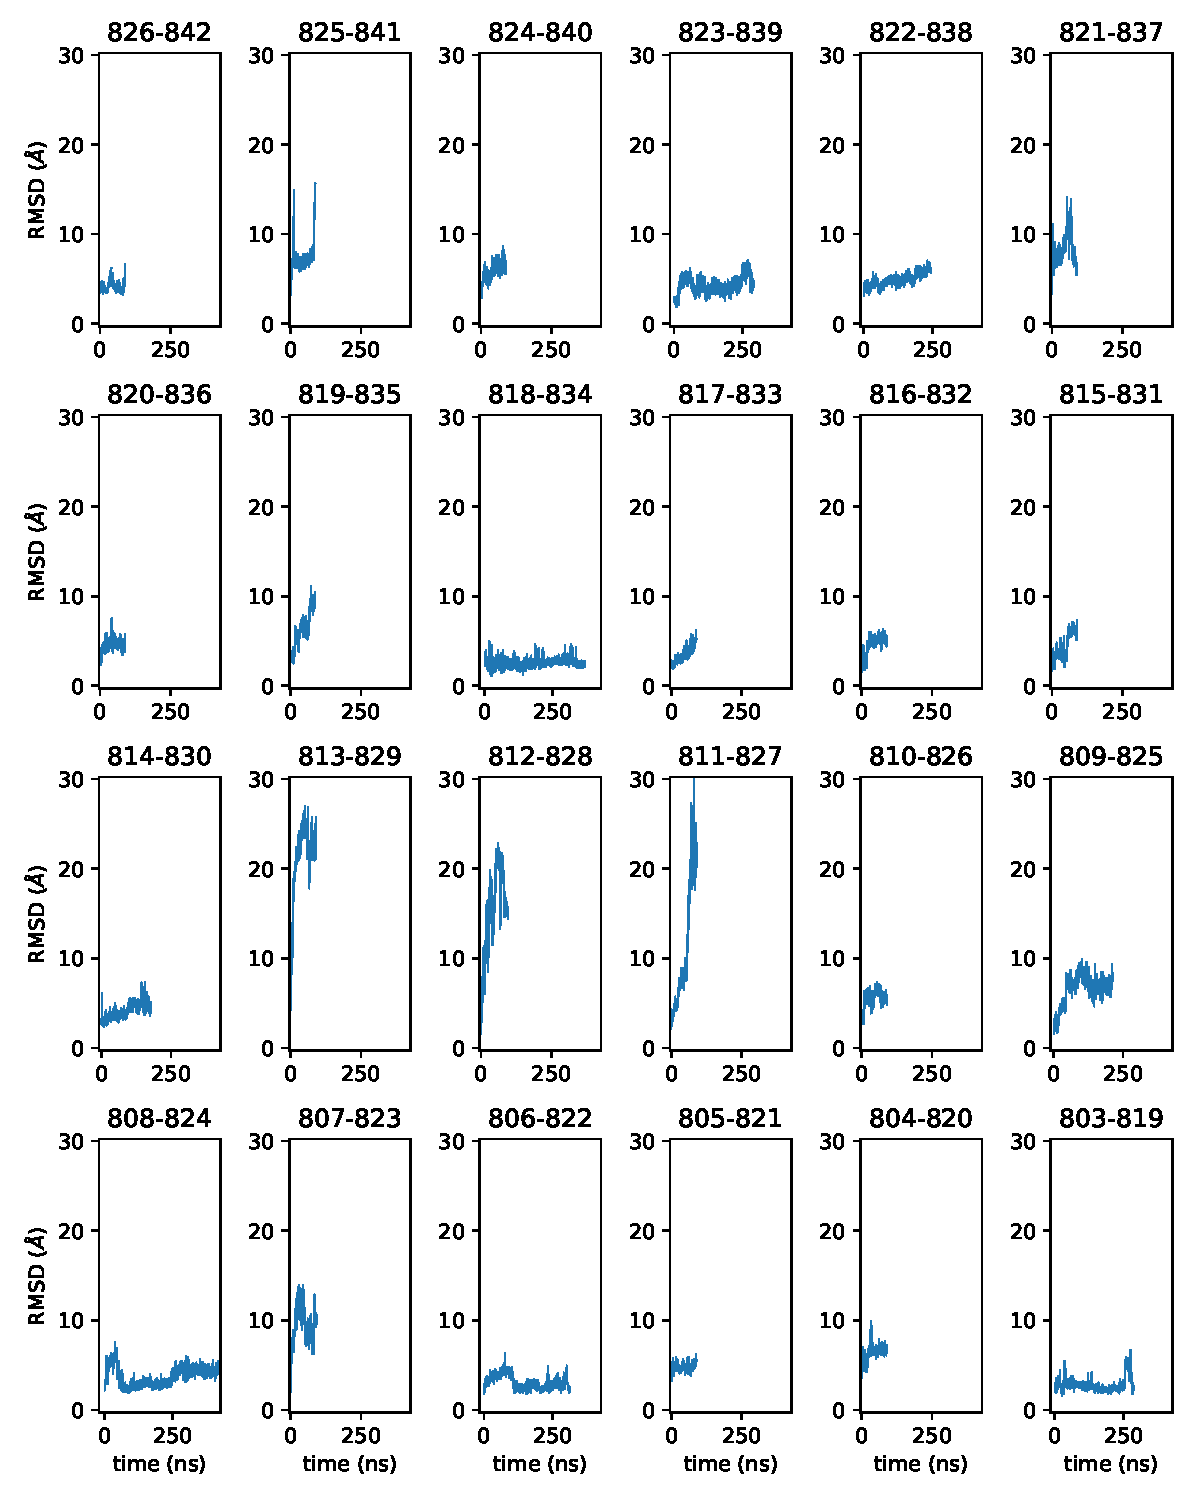
\includegraphics[width=\textwidth]{figures/I37R/Figure_S6.pdf}
\label{I37R_S6}
\end{center}
\begingroup
\captionof{figure}[Results from All Tested R-domain Models]{\textbf{Results from All Tested R-domain Models}}{
Root-mean-square deviation (RMSD) after molecular dynamics simulations of 24 models for the 17 unresolved residues of the R domain after the whole system was aligned to the transmembrane domains (TMDs) of the 6MSM structure.
}
\endgroup

\begin{center}
	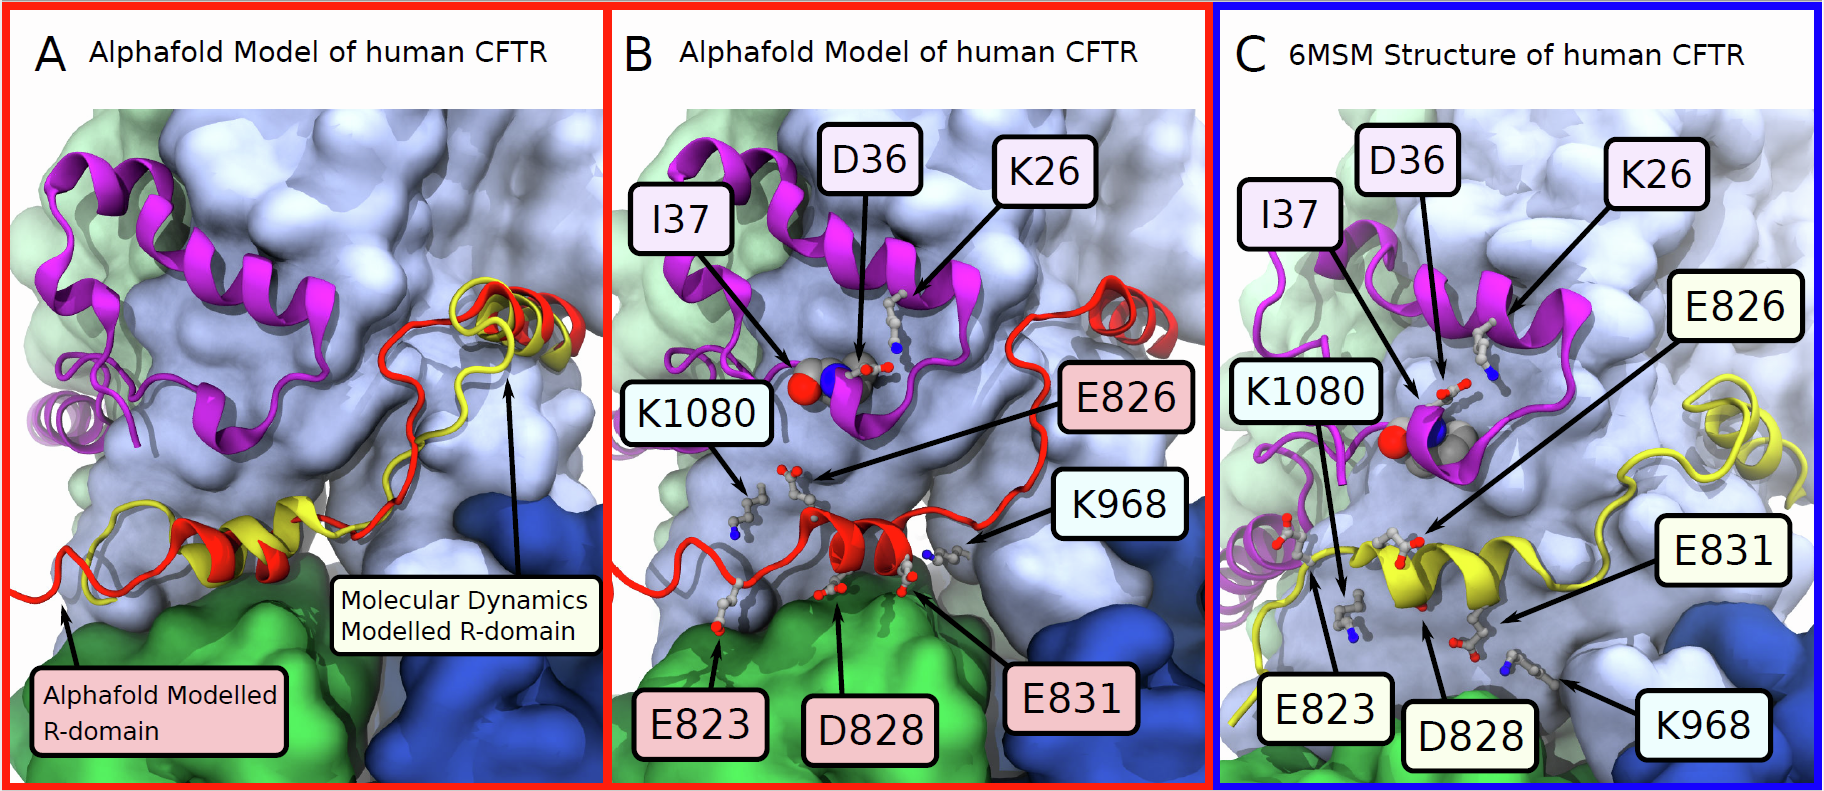
\includegraphics[width=\textwidth]{figures/I37R/S7.png}
\label{I37R_S7}
\end{center}
\begingroup
\captionof{figure}[A comparison between the prediction of the structure of human CFTR by
Alphafold2 and the modelled segment of the R domain]{\textbf{A comparison between the prediction of the structure of human CFTR by Alphafold2 and the modelled segment of the R domain}}{
	Panels with red border indicate the background model in that panel is the Alphafold2 prediction, while the panel with blue border indicates the background model is that of 6MSM, the experimentally derived cryo-EM structure of human CFTR. The MD derived model of the R domain is coloured yellow while the Alphafold2 derived R domain is coloured red. (A) A closeup visualisation of the alignment between the Alphafold2 predicted R domain and the MD based prediction. This figure showed the agreement between the prediction of Alphafold2 and the MD model. The mouse, rat, human and zebrafish CFTR structures in the Alphafold2 database display the same tertiary structure, linking the helical R domain segment closest to the lasso motif, to the beginning of TMD2. This is consistent with the assignment of L818-F834 to the unknown segment of the 6MSM model using MD. (B) The placement of important charged sidechains in the structure predicted by Alphafold2. (hCFTR Alphafold2 model: https://alphafold.ebi.ac.uk/entry/P13569) (C) The placement of important charged sidechains in the 6MSM model, including the modelled helix.
}
\endgroup


\begin{center}
	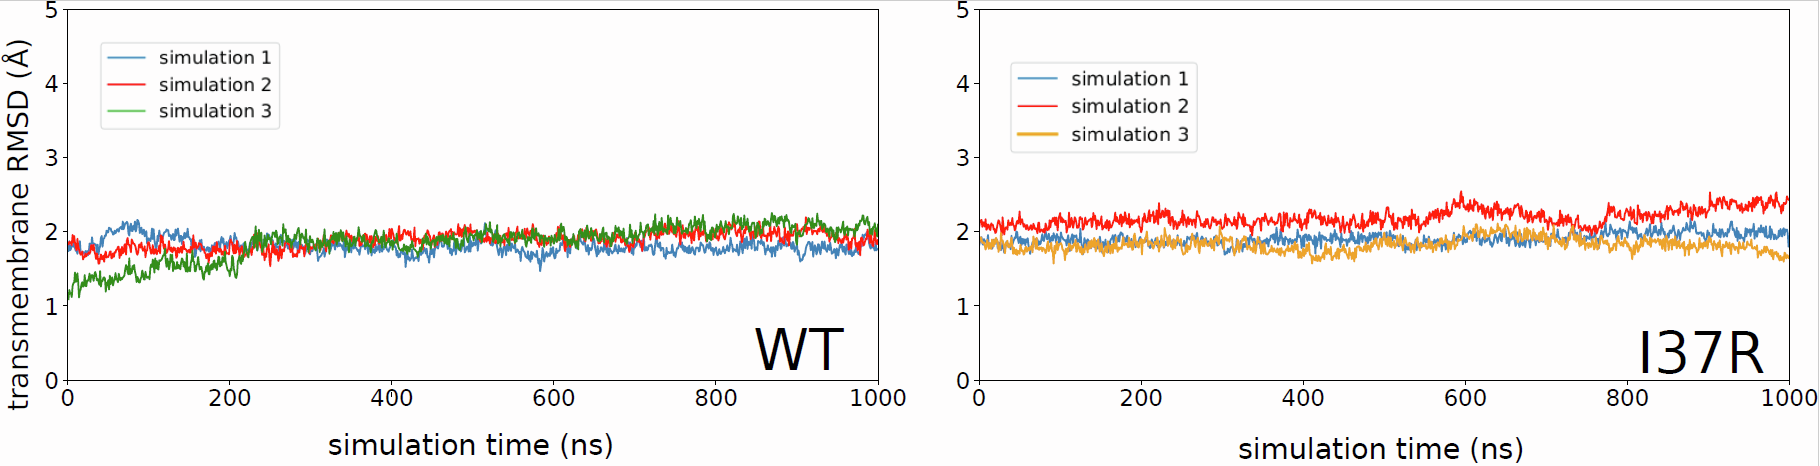
\includegraphics[width=\textwidth]{figures/I37R/S8.png}
\label{I37R_S6}
\end{center}
\begingroup
\captionof{figure}[Comparison between the stability of the transmembrane domains in I37R-
CFTR and WT-CFTR at 310K. ]{\textbf{Comparison between the stability of the transmembrane domains in I37R-
	CFTR and WT-CFTR at 310K. }}{
	 Throughout the microsecond simulations, the transmembrane domain of I37R-CFTR did not deviate significantly from the WT-CFTR indicating no allostery in the transmembrane domains of the I37R mutation. The data coloured orange denotes the simulation described in detail in the results section.
 }
\endgroup

\section{Method Details}
\paragraph{Intestinal Current Measurement} Superficial rectal mucosa samples (2 – 4 per donor) were freshly obtained using biopsy forceps (CK Surgitech NBF53-11023230) and placed in cold RPMI1640 media (Sigma R5886) with 5\% FBS. Intestinal current measurements were performed under voltage-clamp conditions using VCC MC8 Ussing chambers (Physiologic Instruments, San Diego, CA) \cite{dejonge2004, derichs2010, li2004}. Biopsy tissues were bathed in Ringer solution containing (mM)\: 145 NaCl, 3.3 K$_2$HPO$_4$, 0.4 K$_2$HPO$_4$, 10 D-Glucose, 10 NaHCO$_3$, 1.2 MgCl$_2$ and 1.2 CaCl$_2$. Ringer solutions were continuously gassed with 95\% O2-5\% CO2 and maintained at 37$^\circ$C. 10 $\mu$M indomethacin was added to both apical and basal chambers, and tissues were stabilised for 40 min. Tissues were then treated with pharmacological compounds (in order): 100 $\mu$M amiloride (apical) to inhibit epithelial sodium channel (ENaC)-mediated Na+ flux, 10 $\mu$M forskolin + 100 $\mu$M IBMX cocktail (apical and basal) to induce cAMP activation of CFTR, 100 $\mu$M carbachol (basal) to increase intracellular Ca2+ levels and activate basolateral Ca2+-dependent K+ channels and 100 $\mu$M bumetanide (basal) to inhibit basolateral Na+/K+/2Cl- (NKCC) co-transporter.

\paragraph{Forskolin-Induced Swelling Assay} Passage 3-15 organoids were seeded in 96-well plates, in 4 $\mu$l 70\% matrigel droplet per well containing \~25–30 organoids. The next day, organoids were incubated with 1.84 $\mu$M calcein green (Thermo Fisher Scientific C3100MP) for at least 30 min prior to addition of fsk at 0.02, 0.128, 0.8 or 5 $\mu$M concentrations, to determine cell viability. For CFTR potentiation, a single potentiator (3 $\mu$M VX-770 or 3 $\mu$M G1837 or 50 $\mu$M Gen) or dual potentiators (VX-770+G1837 or VX-770+Gen or G1837+Gen) was added together with fsk. Time-lapse images of organoid swelling were acquired at 10-min intervals for 60 min at 37$^\circ$C using Zeiss Axio Observer Z.1 inverted microscope (Carl Zeiss, Jena, Germany), on an EC Plan-Neofluar 5x/0.16 M27 dry objective. Organoids were pre-incubated with 3 $\mu$M VX-809 or 3 $\mu$M VX-661 or 3 $\mu$M VX-445 or 3 $\mu$M VX-445+18 $\mu$M VX-661 for 24 h prior to FIS for CFTR correction where indicated. Three wells were used per condition and each participant’s FIS experiment was repeated 3 to 4 times.

\paragraph{Quantification of Forskolin-Induced Swelling} Organoid swelling was quantified using a custom-built script. A segmentation strategy implemented using ImageJ/Fiji was performed on brightfield images. The raw image was processed with a gaussian blur (s=1.3) to reduce noise. After the directionality and magnitude of the local gradient was identified, pixels were classified as either ‘Background’, ‘Ridge’, ‘Valley’, ‘Rising’ or ‘Falling’ dependent on their neighbouring pixels along the previously calculated local directionality. Clean-up filters were applied that remove noise and small objects, such as ridges that only touched background pixels, and erosions to decrease rising and falling edges to better approximate object boundaries (‘Peaks’). A size exclusion was applied that would discriminate debris in the sample preparation from organoids of interest. This segmentation strategy was used to identify area covered by organoid at each time point. The total surface area of organoid at 10-min intervals over 60 min post-fsk stimulation were calculated and normalized against t=0 to render the relative amount of swelling from t=0. The area under the curve, AUC (calculated increase in organoid surface area from t=0 to t=60; baseline=100\%) was then calculated using GraphPad Prism software.

\paragraph{Quantification of CFTR-Mediated Ion Transport in Organoid-Derived Monolayers} Short circuit current (Isc) measurements were performed under voltage-clamp conditions using VCC MC8 Ussing chambers (Physiologic Instruments, San Diego, CA). Cells were bathed in 20 mM HEPES buffered-Ringer solution containing (mM): 120 NaCl, 0.8 K$_2$HPO$_4$, 5 D-Glucose, 1.2 MgCl$_2$ and 1.2 CaCl$_2$. Ringer solutions were continuously gassed with 95\% O2-5\% CO2 and maintained at 37$^\circ$C. 10 $\mu$M indomethacin was added to both apical and basal chambers and cells were stabilised for 15 min. Cells were then treated with pharmacological compounds (in order): 100 $\mu$M amiloride (apical) to inhibit epithelial sodium channel (ENaC)-mediated Na+ flux, vehicle control 0.01\% DMSO or 10 $\mu$M G1837 (apical) to potentiate cAMP-activated currents, 5 $\mu$M forskolin (basal) to induce cAMP activation of CFTR, 30 $\mu$M CFTRinh-172 (apical) to inhibit CFTR-specific currents and 100 $\mu$M ATP (apical) to activate calcium-activated chloride currents. Isc in response to forskolin was considered as baseline activity ($\Delta$Isc-Fsk) and Isc in response to forskolin and potentiator ($\Delta$Isc-Fsk+Pot) was used as the measure of modulator response.

\paragraph{Immunofluorescence} A rectal biopsy from a I37R/F508del participant was embedded in Tissue-Tek Optimal Cutting Temperature (OCT) compound (Sakura Finetek, CA) and snap frozen prior to storage at -80$^\circ$C. The frozen biopsy was cut into 4 $\mu$m slice sections, and the sections were fixed in ice-cold methanol for 15 min. Intestinal organoids cultured from the I37R/F508del participant and organoid-derived monolayers cultured from a F508del/F508del participant were fixed in 4\% paraformaldehyde and ice-cold methanol respectively for 15 min. Fixed samples were blocked using IF buffer (0.1\% BSA, 0.2\% Triton and 0.05\% Tween 20 in PBS) with 10\% normal goat serum (Sigma G9023) for 1 h at room temperature before incubation in primary antibodies overnight at 4$^\circ$C. The biopsy section was stained with CFTR (1:50, Abcam ab2784) and E-cadherin (1:100, Cell Signalling 3195) antibodies. Intestinal organoids were stained with Ki67 (1:250, Abcam ab15580) and E-cadherin (1:250, Life Technologies 13-1700) antibodies. Organoid-derived monolayers were stained with ZO-1 (1:250, Life Technologies 61-7300) and E-cadherin (1:250, Life Technologies 13-1700) antibodies. On the following day, samples were washed with IF buffer 3 times, 5 min each and incubated with Alexa Fluor conjugated secondary antibodies (1:500, Life Technologies A-11029, A-21329) for 1 h at room temperature. Samples were mounted with Vectashield hardset antifade mounting medium containing DAPI (Vector Laboratories H-1500). Images were acquired using Leica TCS SP8 DLS confocal microscope (Leica Microsystems, Wetzlar, Germany), either on a 63x/1.4 or a 20x/0.75 objective. Images were processed using ImageJ (National Institutes of Health, Bethesda, MD).

\paragraph{Western Blotting} Intestinal organoids were lysed with TNI lysis buffer (0.5\% gepal CA-630, 50 mM Tris pH 7.5, 250 mM NaCl, 1 mM EDTA) \cite{pankow2015} containing protease inhibitor cocktail (Roche 04693159001) on ice for 30 min. Lysates were then sonicated using the Bioruptor Pico (Diagenode, Li\`ege, Belgium) at 4$^\circ$C for 20 cycles of 30 sec on and 30 sec off. Lysates were spun down at 14,000 rpm at 4$^\circ$C for 20 min and protein concentrations were determined using the BCA Protein Assay Kit (Thermo Fisher Scientific 23225). Lysates (100 $\mu$g per sample) were separated using NuPAGE 3 – 8\% Tris-Acetate gels (Thermo Fisher Scientific EA0375BOX) at 100 V for 30 min, followed by 150 V until separation was complete. Proteins were transferred onto a nitrocellulose membrane using wet transfer at 20 V for 1 h at RT. The membrane was then incubated in 5\% non-fat dry milk in phosphate-buffered saline containing 0.1\% Tween (PBST) for 1 h at RT. CFTR bands were detected using anti-CFTR antibody 596 (1:500; University of North Carolina, Chapel Hill and Cystic Fibrosis Foundation) incubated at 4$^\circ$C overnight. Protein bands were visualised using ECL Select detection reagent (Cytiva RPN2235) on the ImageQuant LAS 4000 (GE Healthcare, Chicago, IL). Calnexin was used as the loading control, detected using anti-calnexin antibody (1:1000; Cell Signalling Technology 2679). Protein band densitometry was performed using ImageJ (National Institutes of Health, Bethesda, MD). CFTR maturation in I37R/F508del and F508del/F508del organoids were estimated by measuring the level of mature mutant CFTR (band C) as a percentage of mature CFTR from WT organoids (\% normal CFTR) \cite{vangoor2014}.

\paragraph{In Silico System Composition} A 1-palmitoyl-2-oleoyl-sn-glycero-3-phosphocholine (POPC) bilayer was generated using the VMD membrane builder plugin (Humphrey et al., 1996) in which a model based on the phosphorylated human CFTR channel (PDB ID: 6MSM) was embedded \cite{zhang2018a}. The system was solvated with TIP3P water and neutralised with 0.15 M of potassium chloride ions \cite{mark2001}. The WT-CFTR system included 236 POPC molecules, 128 potassium ions, 140 chloride ions and 44503 water molecules.

\paragraph{Extended 6MSM Structure: Modelling the Unidentified Section of the R Domain} The 6MSM structure was extended in order to resolve a previously unassigned section in the R domain. The R domain is 227 residues long (F630-H856) and is largely disordered \cite{bozoky2013}. In the 6MSM structure, the sidechains of 17 residues of this domain are labelled “UNKNOWN”, due to inadequate electron density in the region. The first 8 residues are unstructured while the next 9 residues form an alpha helix. The distance between the end of the helix and the first visible residue in TMD2 (T845) is 20 $\mbox{\AA}$ \cite{zhang2018a}. Using VMD’s autopsf plugin \cite{humphrey1996} we populated the side chains of the unknown section. Modeller 9.19 was then used to link the R domain to TMD2 at T845 \cite{sali1993}. 24 possible primary structure alignments of this region were simulated. The Root Mean Squared Deviation (RMSD) of the backbone alpha carbon atoms of the extended section with respect to the 6MSM structure was calculated over 300 ns of MD simulations. The most stable alignment was chosen from the lowest RMSD compared to the 6MSM structure. The most stable configuration was capped with the neutral forms of the C and N termini and incorporated into our CFTR model. Four other missing loops namely residues 410-434, 890-899, 1174-1201, 1452-1480 were reconstructed using Modeller 9.19, based on visual analysis and the lowest discrete optimised protein energy (DOPE) score \cite{shen2006}. The N and C termini of the CFTR model were capped with the physiological, charged termini.

\paragraph{Molecular Dynamics Simulation Protocols} The 6MSM structure carries an engineered mutation to avoid the hydrolysis of the bound ATP, giving it a longer lifetime in the open conformation (E1371Q). This mutation was corrected to match the WT-CFTR sequence using the mutator plugin of VMD. The I37R missense mutation was constructed in the same way. GROMACS v2019.3 with the CHARMM36m forcefield was used for all MD simulations \cite{abraham2015, huang2016}. Minimisation via a steepest descent algorithm was performed until all forces were below 24 kcal/mol/$\mbox{\AA}$. This was followed by relaxation simulations of all heavy atoms in the system starting with a restraint of 10 kcal/mol/$\mbox{\AA}^2$ and then halving this restraint every 200 ps in 15 iterations. Relaxation and production were run with 1 and 2 fs time steps, respectively. Relaxation was followed by 5 ns of equilibration. During relaxation, a Berendsen thermostat and barostat were applied, and for production a Nos\'e-Hoover and Parrinello-Rahman thermostat and barostat were applied respectively \cite{berendsen1984,nose1983,parrinello1981}. To maintain the area per lipid (APL) properties of the POPC membrane at experimental values during production runs, pressure coupling was applied in the z-direction normal to the membrane bilayer while the x-y dimensions of the cubic simulation volume was fixed \cite{klauda2010}. While semi-isotropic pressure coupling better replicates membrane environments \cite{pandit2009}, this constant area approach was adopted to circumvent an issue with GROMACS 2019.3reb (https://gitlab.com/gromacs/gromacs/-/issues/2867). Production runs were extended up to 2 $\mu$s at 310 K with three replicates for all simple MD simulations. The last 1 $\mu$s of the longest simulations for each system were selected for further analysis. This was the longest time feasible to simulate with available computational resources. All RMSDs were calculated using the positions of alpha carbons with reference to the 6MSM experimental structure \cite{zhang2018a}. Analysis scripts were written in python using the MDAnalysis library \cite{gowers2016,michaud-agrawal2011}. Bilayer thickness and area per lipid were calculated with the FATSLiM software package \cite{buchoux2017}.

\section{Acknowledgements}
We thank the study participants and their families for their contributions. We also thank Sydney Children's Hospital's (SCH) Randwick respiratory department especially Leanne Plush, Amanda Thompson, Roxanne Strachan, and Rhonda Bell for the organization and collection of participant biospecimens. SAW is supported by an Australian National Health and Medical Research Council grant NHMRC\_APP1188987. MA acknowledges support of a top-up scholarship from Cystic Fibrosis in Australia. MA and KA are supported by Australian Government Research Training Program Scholarship. We acknowledge for the generous provision of the L-Wnt3A cell line. Computations were performed on the Gadi HPC at the National Computational Infrastructure Center in Canberra and Artemis at the Sydney Informatics Hub in The University of Sydney. We thank Dr John R. Riordan (University of North Carolina– Chapel Hill) and Cystic Fibrosis Foundation for providing anti-CFTR antibody \#596. Support statement: This work was supported in part by an Australian National Health and Medical Research Council grant (NHMRC\_APP1188987), a Rebecca L. Cooper Foundation project grant, a Cystic Fibrosis Australia-The David Millar Giles Innovation Grant, Sydney Children Hospital Network Foundation, and Luminesce Alliance Research grants.

\section{Author Contributions}
Conception and design: SAW and AJ. Recruitment and consent: LF and SAW. Collection of rectal biopsies: CYO and LF. Ion transport assay: NTA. Culturing of organoids: NTA, SLW, and SAW. FIS microscopy: IS, KA, and SLW. FIS scripts: MC and RW. FIS analysis: NTA and SLW. Immunofluorescence microscopy: SLW. Western blot: SLW. Molecular Dynamics: MA, PC, RG, and SK. CFTR sequence alignment: AC. Figure preparation: SLW, MA, NTA, AC, KA, and SAW. Writing – original draft: SLW, MA, and SAW. Review and editing: SAW, KA, RG, SK, and LF with intellectual input from all other authors. Supervision: SAW and SK.

\section{Delcaration of Interests}
SAW is the recipient of a Vertex Innovation Grant (2018) and a TSANZ/Vertex Research Award (2020). Both are unrelated and outside of the submitted manuscript. AJ has received consulting fees from Vertex on projects unrelated to this study. CYO has acted as consultant and is on advisory boards for Vertex pharmaceuticals. These works are unrelated to this project and manuscript. All other authors declare no conflict of interest.

%=======================================================================================%
\chapter{Molecular Dynamics and Theratyping in Airway and Gut Organoids Reveal R352Q-CFTR Conductance Defect}
\label{chap:r352q}
\chapquote{Cells have a mind of their own} {-Shafagh Waters (personal communication)}

\section*{\centering Abstract} 
A significant challenge to making targeted CFTR modulator therapies accessible to all individuals with cystic fibrosis (CF) are many mutations in the CFTR gene that can cause CF, most of which remain uncharacterized. Here, we characterized the structural and functional defects of the rare CFTR mutation R352Q – with potential role contributing to intrapore chloride ion permeation – in patient-derived cell models of the airway and gut. CFTR function in differentiated nasal epithelial cultures and matched intestinal organoids was assessed using ion transport assay and forskolin-induced swelling (FIS) assay respectively. CFTR potentiators (VX-770, GLPG1837 and VX-445) and correctors (VX-809, VX-445 +/- VX-661) were tested.  Data from R352Q-CFTR were compared to that of twenty participants with mutations with known impact on CFTR function. R352Q-CFTR has residual CFTR function which was restored to functional CFTR activity by CFTR potentiators but not the corrector. Molecular dynamics (MD) simulations of R352Q-CFTR were carried out which indicated the presence of a chloride conductance defect, with little evidence supporting a gating defect. The combination approach of in vitro patient-derived cell models and in silico MD simulations to characterize rare CFTR mutations can improve the specificity and sensitivity of modulator response predictions and aid in their translational use for CF precision medicine.


\smallskip
%\begin{figure*} [h]
%	\begin{center}
%		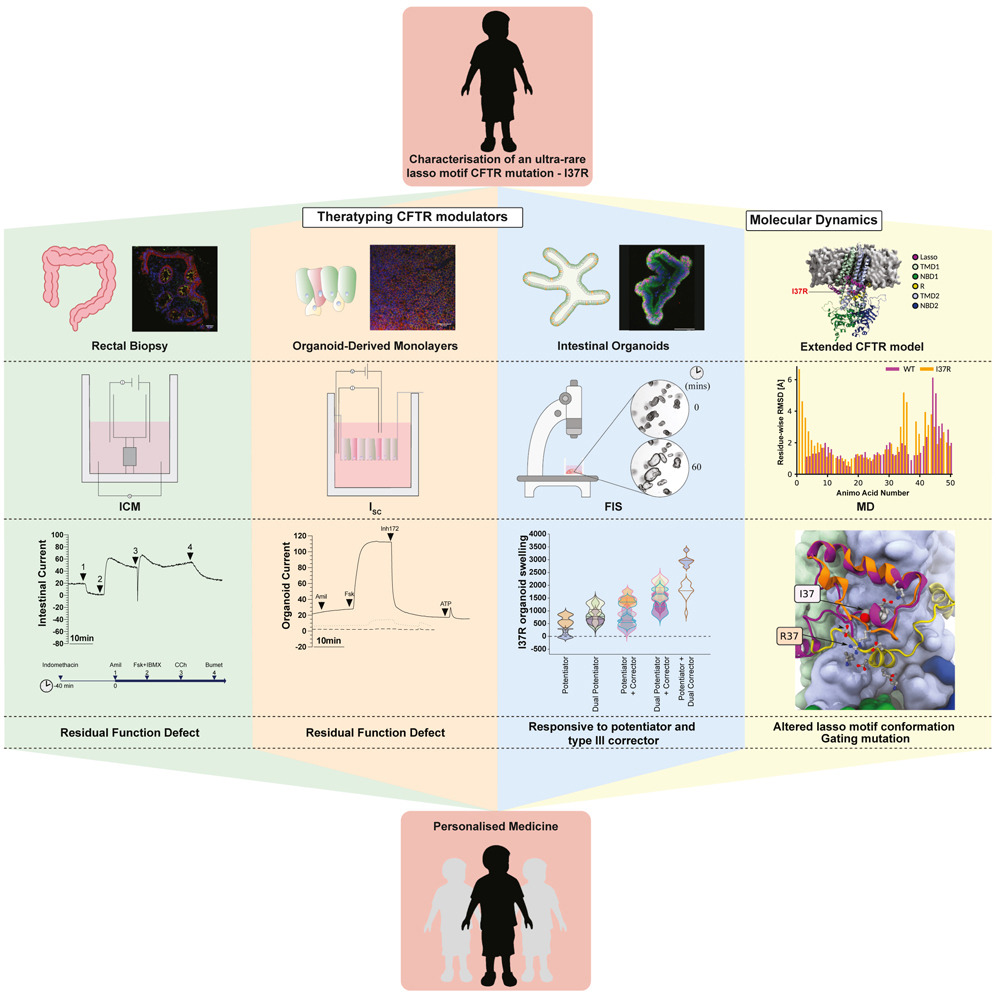
\includegraphics[width=0.80\textwidth]{figures/I37R/graphical_abstract.jpg}
%	\end{center}
%	\captionsetup{singlelinecheck = false, justification=raggedright}
%	\caption[Graphical Abstract. Integration of in silico and in vitro experiments for personalised medicine] {\textbf{Graphical Abstract. Integration of in silico and in vitro experiments for personalised medicine}}{}
%	\label{i37r_graphical_abstract}
%\end{figure*}

\section{Introduction}
Cystic fibrosis (CF), a rare, life-limiting disorder affecting ∼90,000 individuals worldwide (1), results from a malfunction in the cystic fibrosis transmembrane conductance regulator (CFTR) protein. CFTR functions as a cAMP-stimulated anion channel (2). Chloride ions diffuse through the CFTR channel pore, causing a charge imbalance that is corrected by the flux of sodium ions through sodium channels (2). The resultant ion imbalance causes osmosis of water into the extracellular space. More than 2,000 variants in the CFTR gene are known. CFTR mutations are grouped into six major classes based on their functional defects in protein synthesis (I); intracellular maturation, processing, or folding (II); channel gating (III) or conductance activity (IV); diminished quantity (V); and diminished stability (VI) (3).

CFTR modulators can restore mutant CFTR protein function (4). Two subclasses of modulators are in current clinical use, though approval varies between countries. Potentiators such as ivacaftor (VX-770|Kalydeco; Vertex Pharmaceuticals) increase CFTR channel gate opening. Correctors such as lumacaftor (VX-809), tezacaftor (VX-661), and elexacaftor (VX-445) increase delivery of misfolded CFTR to the cell surface. VX-809 and VX-661 are type I correctors that work by stabilizing the NBD1–TMD1 and/or NBD1–TMD2 interface by binding directly to TMD1 (5, 6). VX-445 is a type III corrector that directly stabilizes NBD1 and has been shown to have copotentiator activity (7–10). Combination therapies of potentiator and corrector(s) (Orkambi, Symdeko, Trikafta; Vertex Pharmaceuticals) are approved for use in patients with CF homozygous for F508del, the most common CFTR mutation (11–13). Trikafta is also approved for patients with CF who are heterozygous for F508del (11). The remaining patients with CF are either compound heterozygous or homozygous for mutations other than F508del, only some of which are approved for treatment with modulator therapy (14). A large number of CFTR mutations are not approved for modulator therapy, because their exact mechanism of CFTR dysfunction and/or responsiveness to modulator therapy is often unknown. Traditional randomized clinical trials of modulators to identify modulator-responsive patients with CF with rare CFTR mutations are costly, time-consuming, and impractical (15).

A major breakthrough in the field of CF has been the development of two preclinical patient- and organ-specific cell models (16–18). Both models are used in functional assays that allow rapid quantitative measurements of CFTR function. Differentiated airway epithelial cells are used in transepithelial ion transport assays (short circuit current [Isc]) (19). Intestinal organoids are used in forskolin (Fsk)-induced swelling (FIS) assays (20). Each serves as a personalized functional model of the patient’s CFTR mutation and response to modulators. However, how cell models of the airway compare with those of the gut created from the same patient is not well understood. Mean changes in CFTR function in vivo correlate with the CFTR rescue assessed via the Isc and FIS assays in cell models of subjects with the same mutations (17, 19). In addition, cell model responses in subjects with ultrarare mutations have successfully predicted clinical benefit (21–23). Results so far support the use of patient-derived cell models to guide personalized treatment (24).

We established human nasal epithelial cell (hNEC) cultures from 11 participants with wild-type functioning CFTR (WT/WT) and 10 participants with CF. The participants with CF included five participants with known and characterized CFTR folding/maturation defects (F508del/F508del), three with a CFTR synthesis defect (G542X/F508del), and one with a CFTR gating defect (G551D/F508del). The results from these CFTR mutations with a known impact on CFTR function were used as a reference and were compared with the results from one participant with the R352Q/F508del CFTR genotype. We also created matched intestinal organoids from seven participants with CF and one WT-CFTR control participant (see Table E1 in the data supplement). R352Q, a rare CFTR mutation in the CFTR channel pore, was chosen because it has been characterized in heterologous systems but is yet to be tested in a patient-derived model. Single-channel and whole-cell patch-clamp studies have demonstrated R352 to be a molecular determinant of anion selectivity and permeability in the CFTR channel pore (25). Our aims were to assess CFTR baseline activity and CFTR modulator response in Isc and FIS assays. Potentiator agents VX-770 and GLPG1837 (a potentiator in clinical trials; hereafter G1837) were tested individually and in combination with a CFTR protein-folding corrector VX-809. The effect of VX-445 as a potentiator (acute treatment) and corrector (chronic treatment) monotherapy, as well as part of triple combination therapy VX-445+VX-661+VX-770 (Trikafta) were assessed in FIS assays. In addition, to gain a complementary and better understanding of the effect of R352Q mutation on CFTR function, in silico structural atomistic modeling and molecular dynamics simulations were performed. Some of the results of these studies have been reported previously in the form of a preprint (\href{https://doi.org/10.1101/2021.08.11.456003}{https://doi.org/10.1101/2021.08.11.456003}).


\section{Results}
\subsection{R352Q-CFTR Baseline Activity and Response to CFTR Modulators in Nasal Epithelial Cells}
Mature, differentiated hNECs were pseudostratified (Figure 1A) and had functional beating cilia (CBF, 6.2 ± 0.1 Hz) (Figure 1B, Video 1) and intact junction integrity (Figure 1A) (transepithelial electrical resistance, ≥170 Ω·cm2; Figure E1A). To assess ion transport, Isc measurements were performed (Figures E1B–E1D). We first determined the CFTR activity threshold in reference cell models, which were used for comparison with R352Q-CFTR functional activity before and after modulator stimulation. Fsk-stimulated CFTR-dependent anion currents ($\Del$Isc-Fsk) in WT/WT hNECs were 21.2 ± 1.2 $\mu$A/cm2 at baseline (Figures 1C and 1D, Table E2). Baseline $\Del$Isc-Fsk in F508del/F508del hNECs was at 3.4 ± 0.5 $\mu$A/cm2 and was not increased beyond ∼0.8 $\mu$A/cm2 with either potentiator (Figure 1D). Because of the presence of two copies of the same CFTR mutation, we considered that protein expression from each of the F508del alleles was likely to be the same and therefore attributed each allele to equally contribute ∼1.7 μA/cm2 to baseline Fsk-stimulated currents and ∼0.4 μA/cm2 to potentiator-stimulated currents (Table E2). The baseline $\Del$Isc-Fsk of G542X/F508del hNECs was 0.81 ± 0.12 $\mu$A/cm2. Because G542X is a synthesis defect mutation with no functional CFTR protein production, the observed ∼0.81 μA/cm2 is attributed to the F508del allele, which is not considerably different from that calculated from the F508del/F508del hNECs. We thus used these values as a guide to estimate the contribution of the F508del allele to the experimental Isc data of the heterozygous R352Q/F508del participant. In support of this, F508del/WT hNECs were previously shown to have, on average, ∼50\% of Fsk-stimulated currents of WT/WT hNECs, although variability between F508del/WT participants was present (19).

R352Q/F508del hNECs demonstrated baseline CFTR activity of 14.8 ± 1.4 $\mu$A/cm2, an appreciable 70\% of WT-CFTR activity (Figures 1C and 1D, Table E2). Potentiation with VX-770 or G1837 led to a significant (P $<$ 0.01) twofold increase in CFTR activity, reaching 15.2 and 23.5 $\mu$A/cm2 above baseline, respectively (∼140–180\% WT-CFTR activity). This response is similar to the potentiator-stimulated response observed in the reference gating G551D/F508del hNECs. The G551D/F508del hNECs had $\Del$Isc-Fsk of 4.9 ± 0.6 $\mu$A/cm2 at baseline, and treatment with either potentiator caused an approximately twofold increase in CFTR activity above baseline (net increase, VX-770, 3.0 $\mu$A/cm2; G1837, 8.1 $\mu$A/cm2) (Figures 1C and 1D, Table E2). The majority of the response to potentiators in R352Q/F508del hNECs was most likely contributed by the restored R352Q, because the total response is far greater than the 0.4 $\mu$A/cm2 that we estimated to be attributed to the F508del allele (Figure 1D). We conclude that R352Q-CFTR has high baseline activity amenable to potentiator rescue in hNECs.

We next explored whether corrector monotherapy or cotherapy with potentiators increased R352Q-CFTR functional rescue. In F508del/F508del-CFTR cultures pretreated with VX-809, Fsk alone significantly (P $<$ 0.0001) enhanced CFTR-mediated Cl− currents by 3.7-fold, reaching 9.0 μA/cm2 above baseline (Figures 1C and 1D, Table E2). We estimated each of the F508del alleles to equally contribute 4.5 μA/cm2 to this increase in current. VX-809 cotherapy with either VX-770 or G1837 significantly (P $<$ 0.0001) increased the currents stimulated by potentiator monotherapy by ∼10 μA/cm2 (Figure 1D). In G542X/F508del hNECs, treatment with VX-809 resulted in a modest but significant (P $<$ 0.0001) increase in Fsk-stimulated currents by 1.04 $\mu$A/cm2 above baseline (Figures 1C and 1D, Table E2). In G551D/F508del hNECs, VX-809 treatment significantly (P $<$ 0.001) increased CFTR activity by 5.4 μA/cm2 above baseline (Figures 1C and 1D, Table E2). Because G551D mutation does not respond to VX-809 treatment (26), the contribution of the F508del allele was considered to be 5.4 μA/cm2, similar to that calculated from the F508del/F508del hNECs. In addition, VX-809 cotherapy with either VX-770 or G1837 also increased the respective potentiator monotherapy currents by 2.7 μA/cm2 and 3.8 μA/cm2, respectively (Figure 1D). Unlike F508del/F508del-CFTR, the 9.1 μA/cm2 increase in R352Q/F508del CFTR activity from the baseline in response to VX-809 monotherapy was not statistically significant (P = 0.09). VX-809 cotherapy with either potentiator also resulted in a nonsignificant increase in VX-770– or G1837-potentiated CFTR currents by ∼2 μA/cm2 (Figure 1D). Because VX-809 does not rescue R352Q, then R352Q-CFTR is unlikely to have a folding/maturation defect. The modest increase in current with VX-809 treatment was mostly if not fully imparted by the rescued F508del allele in the R352Q/F508del hNECs.

\subsection{R352Q-CFTR Baseline Activity and Response to CFTR Modulators in Intestinal Organoids}

We evaluated CFTR activity in matched intestinal organoids from the same participant with the R352Q/F508del genotype and those participants with reference F508del/F508del, G551D/F508del, and WT/WT genotypes using an FIS assay. To detect baseline and modulator-stimulated CFTR activity in the organoids, swelling was assessed at four Fsk concentrations ranging from 0.02 to 5 $\mu$M. FIS of organoids was dependent on Fsk dose, CFTR genotype, and the individual participant (Figure 2A). At 0.8 $\mu$M Fsk, the optimal concentration for baseline FIS assessment (17), minimal swelling was observed for the F508del/F508del (area under the curve [AUC], 42.8 ± 19.4) and G551D/F508del organoids (AUC, 82.9 ± 20.1) (Figure 2A). R352Q/F508del and WT/WT organoids showed considerably higher FIS at the same 0.8 $\mu$M Fsk concentration, with AUCs of 196.3 ± 19.9 and 578.3 ± 61.6, respectively (Figure 2A).



FIS of intestinal organoids at 0.128 $\mu$M Fsk has been demonstrated to correlate strongly with clinical modulator responses and therefore is used to assess CFTR modulator response in vitro (17). At this Fsk concentration, organoids—independent of CFTR genotype—did not demonstrate FIS greater than AUC of 67.1 (Figures 2B and 2C, Table E3, Figure E2). In F508del/F508del organoids, treatment with either VX-770 or G1837 did not induce any swelling, suggesting no improvement in CFTR activity with potentiator therapy. G551D/F508del organoids showed a modest 1.5-fold increase in FIS after treatment with either potentiator, increasing AUC by 38.9 (VX-770) and 54.2 (G1837) above baseline (Figure 2C, Table E3). In WT/WT organoids, potentiation with both VX-770 and G1837 led to a significant (P $<$ 0.001) increase in FIS, increasing AUC by 580.6 and 594.2 above baseline, respectively (Figure 2C). In R352Q/F508del organoids, potentiation with either VX-770 or G1837 led to a significant increase in FIS, increasing AUC by 234.6 and 910.6 above baseline, respectively (Figures 2B and 2C). G1837 was significantly (P $<$ 0.0001) more effective in increasing FIS when compared with VX-770 in R352Q/F508del organoids, but not in organoids with the other CFTR genotypes, wherein the efficacy of the potentiators did not significantly differ from each other (Figure 2C, Table E3). Consistent with previous studies showing that VX-445 potentiates CFTR activity but is less potent than VX-770 (7–9), acute treatment of VX-445 modestly increased FIS in R352Q/F508del organoids by an AUC of 90.6 above baseline, lower than the AUC of 234.6 above baseline observed with VX-770 treatment (Figures 2B and 2C). As expected, acute treatment of VX-445 did not induce swelling in F508del/F508del organoids. These data indicate that R352Q has residual CFTR function and is responsive to VX-770 and G1837.

We next determined the effect of VX-809 monotherapy and cotherapy in R352Q/F508del organoids. In reference F508del/F508del and G551D/F508del organoids, VX-809 monotherapy at 0.128 $\mu$M Fsk concentration did not yield a significant change in FIS, with a net increase in AUC $\leq$ 30.4 above baseline (Figure 2C, Table E3, Figure E2). In F508del/F508del organoids, VX-809 cotherapy with either VX-770 or G1837 caused a significant (P $<$ 0.01) increase in FIS compared with potentiator monotherapy, with a net increase in AUC of 189.3 and 145.6, respectively (Figure 2C, Table E3). In contrast, no additional increase in FIS was observed in G551D/F508del organoids after cotherapy with VX-809 and either potentiator (Figure 2C). Similar to the reference F508del/F508del organoids, no change in FIS was observed in the R352Q/F508del organoids at 0.128 $\mu$M Fsk with VX-809 monotherapy. The net increase in AUC was 17.7 above baseline (Figures 2B and 2C, Table E3). VX-809 cotherapy in R352Q/F508del organoids followed the same trend as the F508del/F508del organoids but with a larger magnitude of response. VX-809 cotherapy with VX-770 or G1837 increased FIS beyond each respective monotherapy by 355.2 and 459.7 (Figures 2B and 2C).

The effect of VX-445 monotherapy as a corrector and VX-445+VX-661+VX-770 (Trikafta) triple combination therapy were tested in R352Q/F508del and F508del/F508del organoids. Similar to VX-809 monotherapy, VX-445 monotherapy at 0.128 $\mu$M Fsk induced minimal FIS in R352Q/F508del and F508del/F508del organoids, increasing AUC by 101.3 and 15.2 above baseline, respectively (Figures 2A–2C). In contrast, triple combination therapy VX-445+VX-661+VX-770 significantly induced FIS in R352Q/F508del and F508del/F508del organoids, increasing AUC by 2,913 and 3,173 above baseline, respectively. Because VX-445+VX-661+VX-770 primarily targets F508del folding and processing defects, the lower magnitude of CFTR correction in R352Q/F508del organoids than in F508del/F508del organoids supports our hypothesis that R352Q is unlikely to have folding and processing defects and that the functional correction observed is likely attributed to the F508del mutation.

\subsection{Correlation of CFTR Modulator Response in hNECs with Participant-matched Intestinal Organoid Swelling Assay Outcomes}

We compared the CFTR modulator response as determined by ion transport in hNECs and FIS in intestinal organoids. To determine the amount of modulator-stimulated restoration above the baseline CFTR activity, we subtracted the ΔIsc/AUC values with Fsk alone from those with Fsk plus modulators. A linear positive correlation was observed (r = 0.75; P $<$ 0.0001) (Figure 3A). Participant-to-participant variability was evident (Figure 3B, Figure E3). Among the modulators, an inverse correlation was observed in response to VX-809 monotherapy between the two cell models (r = −0.74) (Figure 3C). Although VX-809 monotherapy significantly increased baseline currents in hNECs, no increase in FIS was detected in the matched organoids (Figure E3). When comparing CFTRinh-172–inhibited currents in hNECs against FIS in intestinal organoids, a similar trend of linear correlation was observed (r = −0.52; P $<$ 0.01) (Figures 3A–3C).

\subsectoin{Maturation of R352Q-CFTR in Nasal Epithelial Cells and Intestinal Organoids}

We next compared CFTR maturation in R352Q/F508del hNECs and intestinal organoids, with and without VX-809 treatment, to understand the distinct response of the two cell models to VX-809 monotherapy (Figure 3D). Robust expression of mature, complex-glycosylated CFTR at ∼160 kD (band C) was detected in both untreated and VX-809–treated hNECs and intestinal organoids. Immature, core-glycosylated CFTR at ∼130 kD (band B) was not present. This validates our functional data by showing the presence of mature CFTR channels on the cell surface in R352Q/F508del hNECs and intestinal organoids, which can therefore elicit residual CFTR function and also respond to potentiator (acts on protein at the cell surface). Mature CFTR in intestinal organoids migrated slightly farther (lower molecular weight) than the hNECs, likely because of different processes of CFTR glycosylation in different tissues, which has been reported previously (27). Treatment with VX-809 did not further increase the levels of mature CFTR relative to the untreated control in both hNECs (densitometry/×104 of 2.2 vs. 2.0) and intestinal organoids (densitometry/×104 of 2.9 vs. 3.1). This is consistent with the nonsignificant or lack of functional rescue with VX-809 monotherapy in R352Q/F508del hNECs and intestinal organoids, respectively. It is noted that the intestinal organoids expressed a higher abundance of mature CFTR protein relative to the hNECs (∼1.5 times), consistent with known CFTR enrichment in the human gallbladder, intestine, and pancreas (28, 29).

\subsection{Molecular Dynamics Simulations and Free Energy Calculations Reveal the Dysfunction of the R352Q Mutant}


We next characterized the structural defect of R352Q-CFTR with molecular dynamics (MD) simulations, using an extended model of the phosphorylated, ATP-bound human CFTR (30). In line with the previously proposed role for R352 in forming a salt bridge (31), it was observed that mutation of the positively charged arginine (R) to neutral glutamine (Q) disrupted the R352-D993 salt bridge in the midsection of the CFTR channel pore (Figure 4A, Figure E4). This salt bridge is a key structural element in CFTR, and its disruption has been shown to impact conductance and gating (31). However, there was no discernible disruption to the R352Q-CFTR channel pore architecture, because the root mean squared deviations of membrane-spanning helices of the R352Q-CFTR were as stable as the WT in microsecond-long MD simulations (Figure 4B). This suggests that the R352Q-CFTR open conformation can remain stable on the submicrosecond time scale necessary for chloride conduction (32). If gating was impacted by the R352Q mutation, longer simulations might be able to decipher any disrupted pore architecture.

Because the R352 residue lines the CFTR channel pore, the R352Q mutation can be expected to affect the conduction of chloride ions (33). This was assessed by determining the path of chloride conduction through the channel and comparing the occupancy of residues along the conduction pathway in WT-CFTR and R352Q-CFTR (Figures 4C and 4D, Video E2). In the WT system, a chloride ion spontaneously enters the pore intracellular gate (34) and diffuses toward K190 and K370 (site I) (Figure 4C). It remains in this site for ∼10 nanoseconds and then spontaneously moves up to the vicinity of R352 and R303 (site II). R248, which is positioned between sites I and II, coordinates the chloride ion movement between these sites. The chloride ion then moves to the vicinity of R134 and K95 (site III), which coordinate chloride diffusion into the outermost section of CFTR. Chloride conduction through the CFTR channel pore does not follow a straight path from pore entry to site III but rather follows a longer, indirect route. This is in contrast to the straight path that ions follow through voltage-gated potassium and sodium channels, which have tight pores that run perpendicular to the membrane (35).

In R352Q-CFTR, chloride ions can enter the channel pore but not as readily as in the WT system. They also generally do not progress as far into the pore as for WT-CFTR. Although multiple chloride ions occupied the WT-CFTR channel pore concurrently, only one chloride ion at a time was observed in the R352Q-CFTR channel pore. The highest occupancy in R352Q-CFTR was found for K1041. The chloride ions that enter the WT-CFTR channel pore stayed mainly in sites I and II, with occupancies of these two sites drastically reduced in R352Q-CFTR compared with WT-CFTR. This reduction in occupancy observed in R352Q-CFTR is due to neutralization of the positively charged R352 side chain, which reduces the affinity of chloride ions to site II. Site III was inadequately sampled to draw conclusions (Figure 4D). Intriguingly, some chloride ions appeared to penetrate site III in both WT- and R352Q-CFTR, which could explain the mild conductance defect observed for R352Q. In addition, in simulations of WT-CFTR, it was observed that D993 alternated contact between R303 and R352 (Figures E4A and E4B). However, in R352Q-CFTR, D993 forms a more stable salt bridge with R303 (Figure E4C), which curtails its ability to coordinate a chloride ion.

The impact of the lower occupancy of sites I and II on chloride conductance was quantified further by comparing the respective free energy profiles obtained from umbrella sampling MD simulations (Figure 4E). To generate the initial path for the umbrella sampling simulations, one chloride ion was constrained at site I and then steered via site II toward R134 in site III, using a moving restraint. The free energy profile calculations followed the protocol described in the Supplemental Materials and Methods of the data supplement. In WT-CFTR, calculation of the free energy profile yielded an energy trough of −4 kcal/mol at site II relative to site I (Figure 4E). This indicates that chloride ions will be attracted to this site. In contrast, in R352Q-CFTR, the free energy profile exhibited an energy barrier of +1 kcal/mol at site II, which will likely hinder chloride conduction. Therefore, in WT-CFTR, a chloride ion in site I will tend to move to site II, whereas such a motion will be suppressed in R352Q-CFTR, resulting in reduced chloride conductance.

\section{Discussion}

%=======================================================================================%
\chapter{Unique S945L-CFTR defect Restored by CFTR Modulator Co-Therapy In Vitro, Which Correlates with In Vivo Biomarkers Post-Therapy}
\label{chap:S945L}

\setcounter{figure}{0}
\renewcommand{\thefigure}{\arabic{chapter}.\arabic{figure}}

\begin{chapquote}{-David Goodwin (personal communication)}
Eventually, you'll realise you're just two days from anywhere.
\end{chapquote}


\section*{\centering Preamble on Formatting} 
The work in the following chapter is part of a publication in preparation for submission to \textit{Frontiers in Pediatrics}. All experiments have been completed and the authors are in the process of writing the manuscript. The computational components of the manuscript have been finalised, and the results are presented here. On the other hand, because the \textit{in vitro} and clinical components of the manuscript have not been finalised, so their results are not included explicitly in the manuscript. Instead they are described in brief and referred to as needed to give the \textit{in silico} results context.

\section*{\centering Abstract} 

Cystic Fibrosis (CF) results from loss of functions mutations to the CF Transmembrane Conductance Regulator (CFTR) gene. A CFTR mutation can produce numerous defects and drugs known as CFTR modulators have been developed to act directly on the protein and restore its function. These drugs have been a breakthrough in the treatment of CF. However, the response of patients to these medications is variable, and there is an urgent need for a personalised approach to their administration. The objective of this study was to elucidate the molecular details of pathogenesis of a rare mutation, S945L through molecular dynamics (MD) simulations and umbrella sampling. These methods discovered a mode of pathogenesis unique to S945L-CFTR, which results in both gating and folding defects. Our simulations were performed in parallel to \textit{in vitro} assays which were used to interrogate the efficacy of modulators in patient specific cellular models. This was followed by a clinical study, which tracked the outcomes of the patient carrying the S945L mutation upon receipt of the recommended medication. The results indicate that the mode of pathogenesis unique to the S945L mutation was responsive in vivo to current generation CFTR modulators. Hence, the presented study demonstrates how patient specific cellular assays can assess the efficacy of modulators in rare mutations and inform clinical practice.


\section{Introduction}
Cystic Fibrosis (CF) is a life-limiting recessive disease \cite{mall2014, elborn2016} caused by mutations in the CF Transmembrane Conductance Regulator (CFTR) gene that result in absent or dysfunctional CFTR protein \cite{rowe2005}. The CFTR protein is a chloride and bicarbonate channel \cite{veit2016} which maintains fluid homeostasis at the apical membrane of epithelial cells \cite{riordan1989} in the lungs, pancreas, liver and intestine \cite{ratjen2015}. CFTR is a complex protein, composed of seven domains. Of primary significance to this study are the Transmembrane Domains (TMDs) and the Regulatory domain (R-domain). TMDs 1 and 2 are composed of six tight bundles of helices which run through the plasma membrane. The proper arrangement of these helices is critical to avoiding a folding defect of the protein \cite{fiedorczuk2022}. The S945L mutation occurs in TMD2 on a helix numbered TM8. When CFTR opens, the TMDs twist in order to form a pore and allow ions to pass through. In the closed state the R-domain wedges between the TMDs, preventing them from twisting to form a pore. During gating, the R-domain is phosphorylated and dislodges from its wedged position and docks against TMD2 \cite{zhang2018}. Regulating the movement of the R-domain has important implications for the gating cycle of the protein \cite{mihalyi2020}.

CF is a monogenic disease and over 2000 unique mutations have been identified in the CFTR gene, yielding a spectrum of CFTR structural defects \cite{deboeck2016}. Of these, 401 mutations have been found to be disease-causing \cite{cftr2}, albeit with heterogeneous clinical phenotypes \cite{bonadia2014}. Whilst not curative, a novel class of targeted therapies (CFTR modulators) have been developed to restore CFTR protein function \cite{awatade2018}. CFTR modulators have two modes of action:  potentiators (ivacaftor, GLPG1837) which open the CFTR channel pore \cite{vangoor2009, accurso2010, yu2012, rosenfeld2018}, and correctors (lumacaftor, elexacaftor, tezacaftor) which assist in CFTR protein folding and trafficking to the cell surface \cite{lopes-pacheco2017, dekkers2016b}. Clinically approved dual therapies, lumacaftor/ivacaftor and tezacaftor/ivacaftor + ivacaftor (Symdeko), as well as triple combination therapy elexacaftor/tezacaftor/ivacaftor + ivacaftor (ETI) improve CFTR function via both these mechanisms \cite{ wainwright2015,rowe2017, middleton2019}. 

ETI is currently the most effective treatment for improving patient lung function, \cite{rowe2017,keating2018} and provides treatment access to more than 90\% of people with CF. However, the clinical response to ETI, as well as other modulators, has been reported to be heterogeneous, even amongst patients with the same CFTR mutation \cite{wainwright2015, boyle2014}. \textit{In vitro} CFTR modulator testing uses patient-derived cells models as a personalised drug screening platform to predict the individual’s response to treatment and characterise the functional defect caused by CFTR mutations. This form of \textit{in vitro} analysis has been permitted by the US Food and Drug Administration (FDA) to inform approval of therapeutics for less common CFTR mutations. 

The diversity of disease-causing mutations and the availability of high resolution CFTR protein structures have led to the ability to study the effects of rare mutations in detail. In this study we have used Molecular Dynamics (MD) combined with Umbrella Sampling (US) to study the stability and dynamics of the S945L-CFTR protein. Our results suggest this mutation causes both a folding defect and a gating defect, due to the destabilisation of a fragment of the R-domain. 

The modelling work was motivated by studies of a patient carrying the S945L/G542X-CFTR genotype. As they are still under preparation, the \textit{in vitro} and clinical results of this study are not presented, but will be described in brief.

The cell models derived from this patient were assessed for their response to various CFTR modulators. It was predicted through these pre-clinical assays that the patient would benefit from combination therapies such as Symdeko, which is a combination of tezacaftor (VX-661), a corrector and ivacaftor (VX-770), a potentiator. After a year on this medication, an increase in lung function was observed in the patient. These clinical results validated the hypothesis generated from the \textit{in vitro} cell models, demonstrating the efficacy of a patient specific approach to the choice of CFTR modulators.
%\cite{wong2022, wong2022a}

This is also consistent with our previous work, which has demonstrated the functional rescue of rare missense mutations by modulators . All observed rescue in the S945L/G542X patient must have been due to the modulation of the S945L-CFTR protein, as G542X is a class I nonsense mutation, which does not respond to modulators  \cite{hamosh1992, valley2019}. S945L is a rare CF-causing CFTR mutation expressed on 167 of 142,036 CFTR alleles worldwide (0.00118\% allelic frequency) and results in pancreatic insufficiency in 40 \% of carriers 11. S945 is situated at the end of transmembrane helix 8 of the CFTR protein, a region known to contribute to ion selectivity \cite{negoda2019} and bind potentiator class CFTR modulators \cite{liu2019}. 

S945L has approval for treatment with Symdeko in the US, Canada, Europe and Australia based on evidence of improved lung function in a Phase III clinical trial of 248 patients (13 patients with S945L) 12 years or older \cite{rowe2017}. While the rescue efficacy of Trikafta has not been assessed for this mutation. Furthermore, although functional characterisation of S945L-CFTR has been performed via molecular studies in heterologous expression Chinese hamster ovary cells and described to interfere with protein folding, as well as gating function \cite{seibert1996}, this has not been validated in patient derived cell models. Molecular dynamics (MD) simulations of the CFTR protein have previously demonstrated the importance of hydrogen bonds on TM8 to the stability of the open state \cite{corradi2018}. Due to its proximity to this region, we believed that the S945L molecular defect might be due to the disruption of interactions that stabilise wild-type (WT) CFTR. This motivated MD simulations and free energy calculations of the S945L-CFTR protein, to characterise its molecular defect.

In parallel with our computational modelling, the mutation was functionally characterised \textit{in vitro} by assessing the response to CFTR modulators via a CFTR-mediated chloride transport assay in S945L/G542X-CFTR patient-derived primary airway epithelial cell models. Various CFTR modulators with different mechanisms of action were tested \textit{in vitro} to characterise S945L-CFTR, leading to the prediction that a combination therapy would give the patient the most benefit. \textit{In vivo}, it was then found that the patient exhibited increased lung function after treatment with the combination therapy Symdeko. This demonstrates the success of a personalised approach to the choice of CFTR modulators. 

\section{Results}

\subsection{In silico characterisation of the Misfunction of S945L-CFTR}
The S945 amino acid is located in TM8, near the membrane surface on the cytoplasmic side of CFTR (Figure \ref{S945L_MD_1}A). Our simulations show that this amino acid plays a structural role by bridging TM8 with adjacent TM7 and R-domain helices. This is facilitated in WT-CFTR by hydrogen bonding to Y852 in the R-domain. Two configurations of this hydrogen bonding were observed in WT-CFTR simulations, indirect hydrogen bonding via a stable, mediating water molecule, or direct hydrogen bonding between S945 and Y852 (Figure \ref{S945L_MD_S1}A). Both states are energetically favourable and keep the Y852 and S945 amino acids in proximity to one another (Figure \ref{S945L_MD_S1}B). The interactions were stable throughout three replicate 2 $\mu$s MD simulations of WT-CFTR, at both a physiological temperature (37$^o$C; Figure \ref{S945L_MD_S2}) and an elevated temperature (77oC; Figure \ref{S945L_MD_1}B and Figure \ref{S945L_MD_S1}A-B). 

In S945L-CFTR, the mutant leucine amino acid (L) lacks the polar sidechain of the WT serine (S), so it cannot form hydrogen bonds (Figure \ref{S945L_MD_1}A). The effects of this change were measured and compared in WT and S945L-CFTR. Compared to WT-CFTR, S945L-CFTR had increased conformational fluctuation in the R-domain elbow, as measured by root mean square deviation (RMSD, Figure \ref{S945L_MD_S3}A-B). This suggested that the S945L mutation decreased the R-domain stability. The instability and loss of the hydrogen bond anchor allowed the R-domain Y852 sidechain in one S945L simulation to physically rotate away from TM8 (Figure \ref{S945L_MD_1}B). Since the R-domain is critical for protein gating, these observed movements and destabilisation of the R-domain suggest that S945L-CFTR is likely to possess a Class III gating defect.

In S945L-CFTR, movement of the R-domain away from its folded conformation was observed in only one of three replicate simulations at 77$^o$C (Figure \ref{S945L_MD_1}B). While this movement was not observed in any of three replicates at physiological temperature (37$^o$C, Figure S2). These results suggested that direct microsecond simulations were not long enough to reliably explore potential pathological conformational changes in S945L-CFTR. We believe the presence of the lipid bilayer near the S945L mutation introduced a kinetic barrier to the expected conformational changes. The slowed movements of the R-domain elbow motivated more investigations into the energetics of this motion by a more rigorous method known as umbrella sampling (US). Here we used a virtual spring to pull apart the alpha carbon atoms of amino acids 945 and 852. As the atoms were pulled away from each other, we measured the force exerted on the spring. This let us calculate how likely the link between Y852 and S/L945 was to break in both WT and S945L-CFTR.

WT-CFTR displayed a free energy surface more stable than S945L-CFTR because of the presence of the S945-Y852 hydrogen bond (Figure \ref{S945L_MD_1}C). The WT-CFTR free energy surface featured a deep local minimum when Y852 and S945 alpha carbons were separated by 9.5 $\mbox{\angs}$. Distances greater than 12 $\mbox{\angs}$ were inhibited in WT-CFTR by high energies of 4.7 kcal/mol, which would not be easily accessible at physiological temperatures. Therefore, WT-CFTR was likely to occupy the deep minimum at 9.5 $\mbox{\angs}$. This indicates the constraining effect of the hydrogen bond between S945 and Y852. The steepness of the local minimum was also implied by the smaller fluctuations observed during the direct simulations, as if bound by a tight spring (Figure \ref{S945L_MD_1}B). These findings indicate that WT-CFTR will remain correctly folded because of its stable network of hydrogen bonds. In contrast, the S945L-CFTR free energy surface showed several shallow local minima between the near-native 9.0 $\mbox{\angs}$ and maximum distance of 13 $\mbox{\angs}$, observed in Figure \ref{S945L_MD_1}B. This free energy surface correlates with the larger fluctuations observed in the direct simulations, as if bound by a weaker spring than WT-CFTR (Figure \ref{S945L_MD_1}B). The small, intervening free energy barriers, which had heights of 2.0 kcal/mol or less, could be overcome at physiological temperatures, causing the protein to misfold. This indicates that S945L-CFTR is likely to spontaneously transition into misfolded conformational states where the R-domain elbow, containing Y852, moves away from TM8. We believe these conformational transitions will give rise to the Class II folding defect observed \textit{in vitro}. 

\begin{center}
	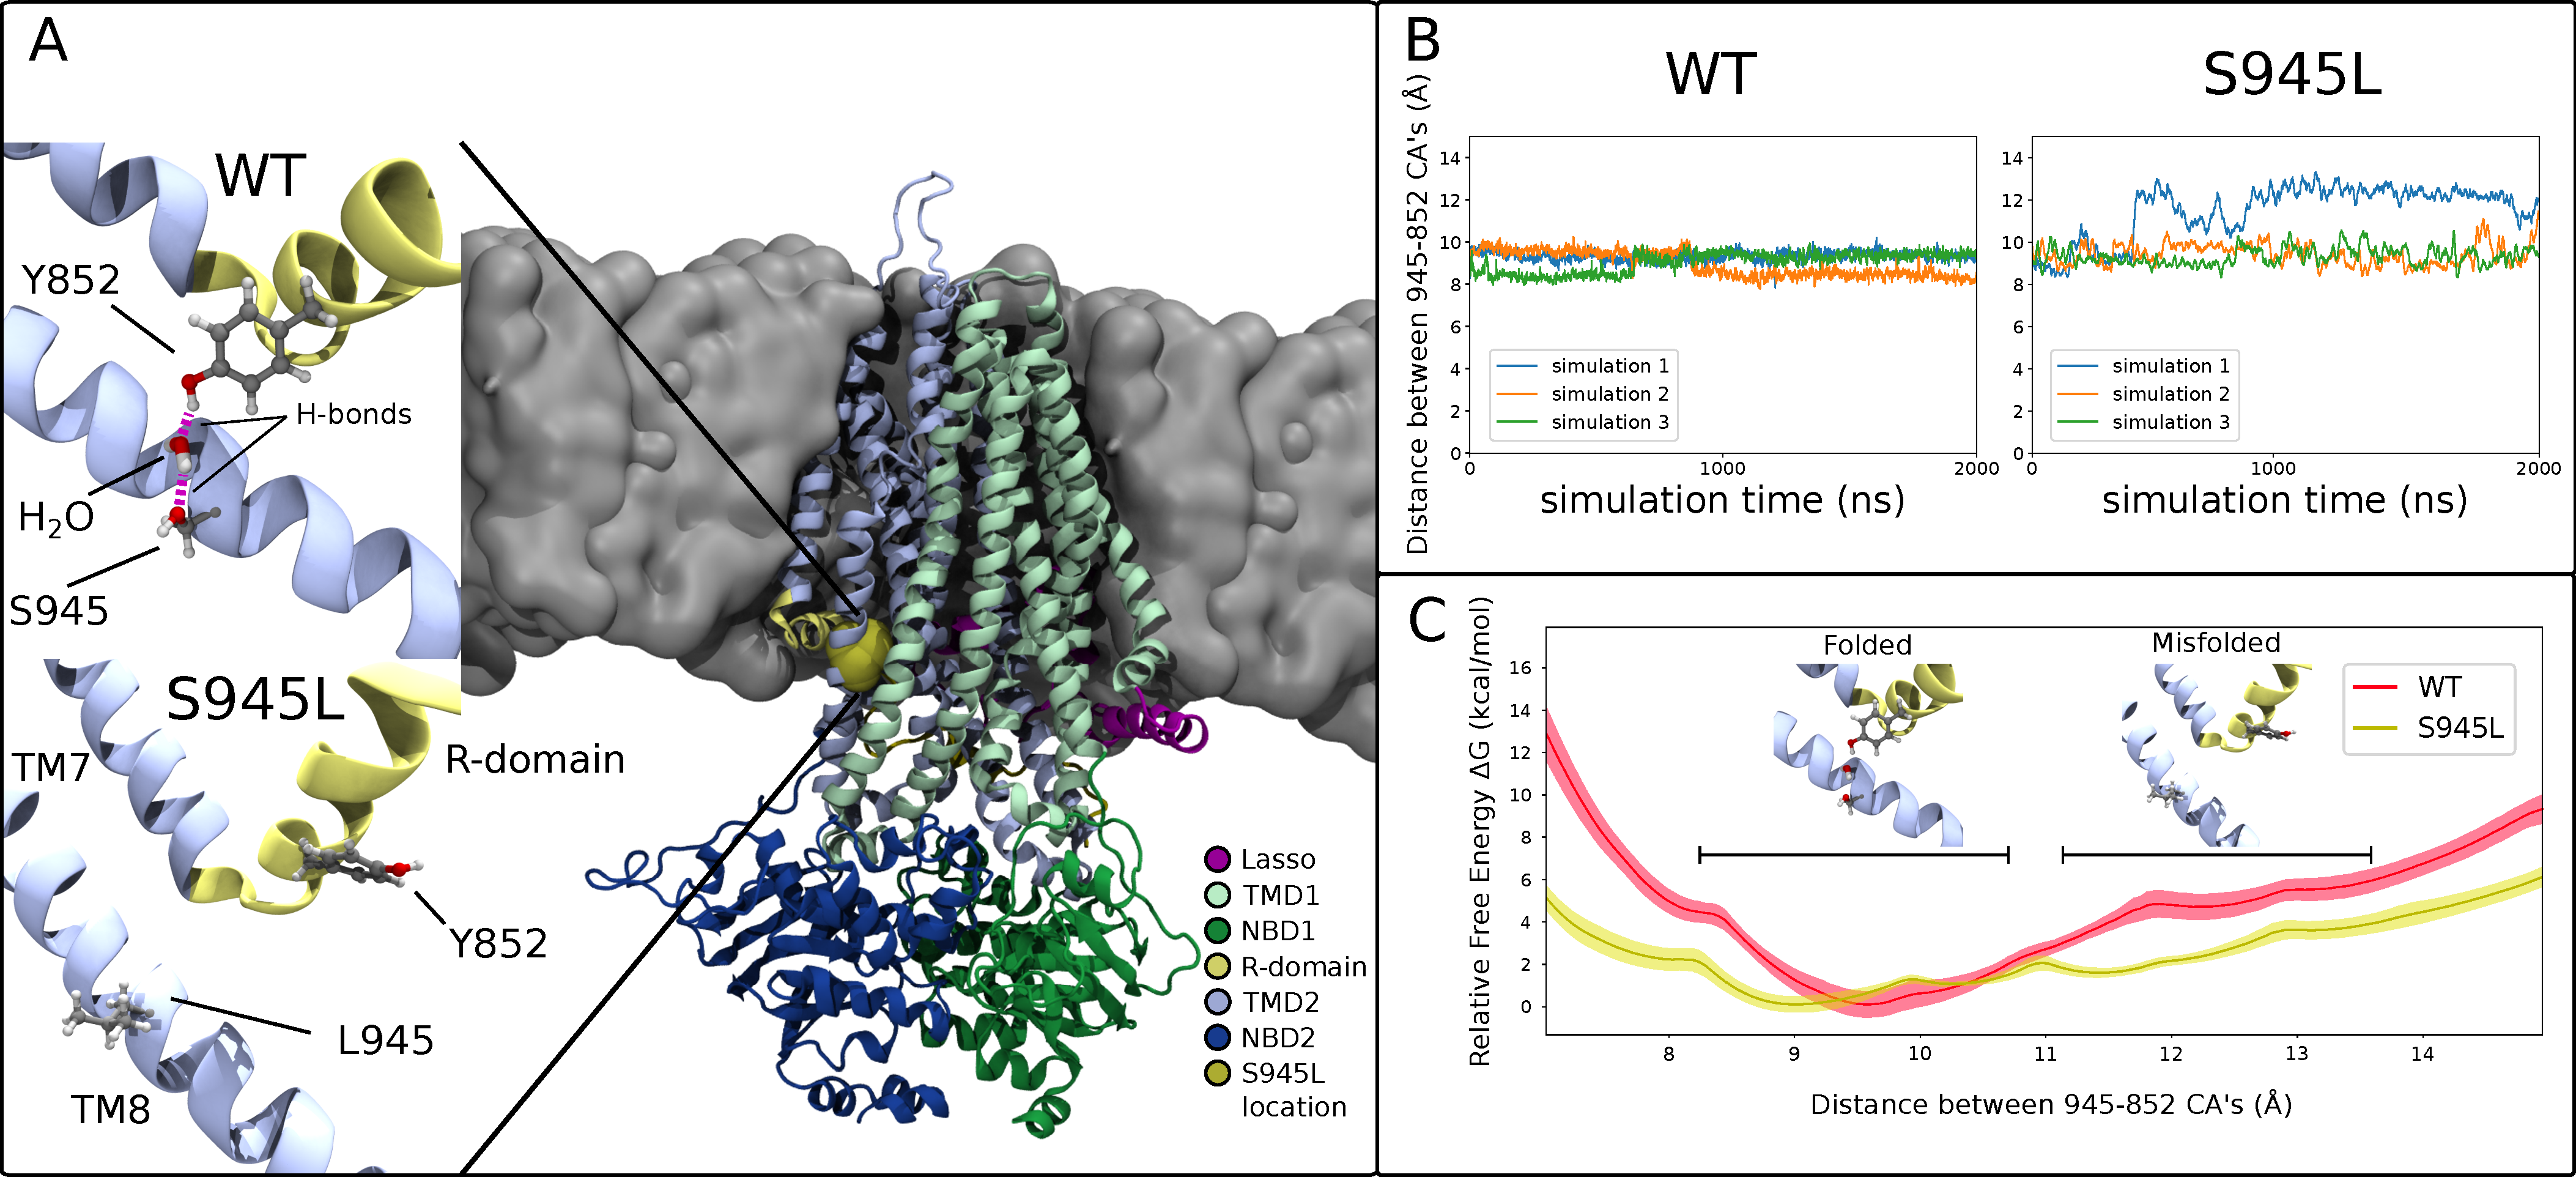
\includegraphics[width=\textwidth]{figures/S945L/Figure1_MD_03082022.pdf}
\end{center}
	\captionsetup{singlelinecheck = false, justification=raggedright}
\begingroup
\captionof{figure}[S945L] {\textbf{S945L}}{A) The location of the S945L mutation in the open structure of CFTR (PDB ID: 6MSM) is indicated with yellow spheres. It is placed between TM8 and the R-domain, the latter domain is critical for the gating of the channel. B) Data from unbiased simulations of WT and S945L-CFTR. A stable network of hydrogen bonds forms spontaneously in simulations 1, 2 and 3 of WT-CFTR. This interaction connects Y852 to S945. In the S945L mutation, the leucine side chain cannot support this hydrogen-bond network. In simulation 1 of S945L-CFTR, after a conformational transition, the amino acids remained at an average distance of 12.2$\pm$0.7 $\angs$. This is significantly further than the average distance in the WT data: 9.1$\pm$0.3 $\angs$. No significant changes were observed in simulations 2 and 3 of S945L-CFTR. C) Results from umbrella sampling, a more computationally rigorous approach, confirm the presence of the conformational change in S945L-CFTR. Distances below roughly 10.5 $\angs$ correspond to a well folded state, while distances larger than 11 $\angs$ appear to correspond to a poorly folded state. In the mutant, there is a shallow free energy minimum at 11.4 $\angs$ with a difference in the energy landscape of 3.2 kcal/mol compared to WT-CFTR at the same location. The presence of this shallow free energy minimum indicates that S945L-CFTR is more likely to misfold than WT-CFTR. }
\label{S945L_MD_1}
\endgroup

\section{Discussion}
We have described in detail the structural and functional CFTR defects caused by the S945L mutation. In silico protein modelling via MD simulations was used to determine the molecular cause of both a folding and a gating defect in S945L-CFTR.  Airway epithelial cell models derived from a participant with S945L/G542X-CFTR were also created and their response to CFTR modulators was tested via functional studies, to characterise their functional defect. The rescue of mutant CFTR was found to then translate to success in the clinic, as the patient carrying this mutation had an increase in lung function following the administration of the recommended therapy.

In our MD simulations of WT-CFTR, a stable network of hydrogen bonds linking Y852 in the R-domain to S945 on TM8 was identified. This interaction was not visible in the cryo-EM structure of the channel, where S945 faced away from Y8528. It is often not possible to resolve such water mediated interactions in cryo-EM structures. This is due to the difficulties in achieving a high enough resolution with experimental structural biology techniques and the dynamic nature of the proteins themselves. The elucidation of this interaction in this study demonstrates the atomistic insight which computational methods can provide into the function of proteins. In simulations of S945L-CFTR, this interaction was disrupted, and our results indicate that the R-domain may move away from TM8 (Figure \ref{S945L_MD_1}B). Due to the importance of the R-domain in gating, we expect that a change to its position will give rise to a gating defect. This is a similar mode of pathogenesis the one observed in the I37R mutation, although it is interesting that it occurs in a different domain in CFTR. Simultaneously, the disruption of this link between two different domains is likely to give rise to a folding defect, as the elbow region will be less likely to fold correctly. Hence, our MD simulations have revealed a unique mode of pathogenesis for the S945L mutation. It is unlikely that other mutations would disrupt this hydrogen bond in the same way. This is another example in a set of MD simulations of the CFTR protein which suggest that CFTR modulators can elicit a response in many missense mutations, each with unique molecular phenotypes \cite{wong2022,wong2022a,billet2020,sabusap2021}. 

The results from clinical and \textit{in vitro} experiments are not shown explicitly, but described here to complement and give context to our MD studies. When tested under basal conditions, the S945L/G542X-CFTR ALI cell models exhibited high residual activity. This indicated the presence of some CFTR protein at the cell surface, suggesting that the S945L mutation produces a mild CFTR folding defect. Monotherapies using either a single potentiator or a single corrector were not able to restore CFTR function to levels which would indicate clinical benefit. However, combination therapies Symdeko and Trikafta were able to restore function in these cell models. This was expected as Trikafta has recently been evaluated in rare class II CFTR folding mutations and variable genotype-specific responses were found \cite{veit2020, laselva2021}. Like the prototypical class II folding mutation $\Delta$F508, S945L has been reported to cause multiple defects including protein maturation, channel gating and conductance \cite{seibert1996}. 

We correlated the \textit{in vitro} drug response of the S945L/G542X-CFTR patient-derived cell models to the patient’s in vivo change in lung function (FEV1) following treatment with the Symdeko. Once the patient was administered Symdeko for 12 months, their lung function improved. These results support the use of personalised primary airway cell models as a valuable tool to study modulator efficacy and predict patient drug response for patients who carry rare mutations which are difficult to study through clinical trials. 

The \textit{in vitro} and clinical studies demonstrate the efficacy of pre-clinical cellular models, while the MD studies demonstrate the rescue of yet another unique molecular defect by CFTR modulators.  

\textit{In vitro}, S945L-CFTR was not found to respond to treatment by a potentiator monotherapy. This is consistent with previous findings. The rescue of S945L-CFTR by correctors has not previously been assessed, but again significant restoration was not observed with this kind of monotherapy. By contrast, combination therapies Trikafta and Symdeko were found to restore function in cellular models. As such, we characterise S945L to incur both CFTR folding and gating defects, which is in support of previous molecular studies performed in heterologous expression CHO cells \cite{seibert1996}, as well as the findings of our MD simulations.

Since the response of different CFTR mutations \cite{laselva2021} to modulators is heterogeneous \cite{wainwright2015,boyle2014}, there is a strong rationale for modulator screening of CFTR in patient-specific cell models. Prediction of CFTR drug response in patient-specific cell models may, in the future, lead to extended approval of CFTR modulators for rare CFTR mutations currently without treatment access. Together with other integrative studies using both MD simulations and \textit{in vitro} functional studies to characterise CFTR mutations and predict drug response in a personalised manner \cite{wong2022,wong2022a,billet2020,sabusap2021}, there is a growing body of evidence that a large number of unique molecular defects may be rescued by CFTR modulators. Further development of patient-specific cell models as a predictive tool could lead to the optimal choice of CFTR modulators to treat each patient.  

\section {Supplementary Information}
\renewcommand{\thefigure}{\arabic{chapter}.S\arabic{figure}}
\setcounter{figure}{0}

\begin{center}
	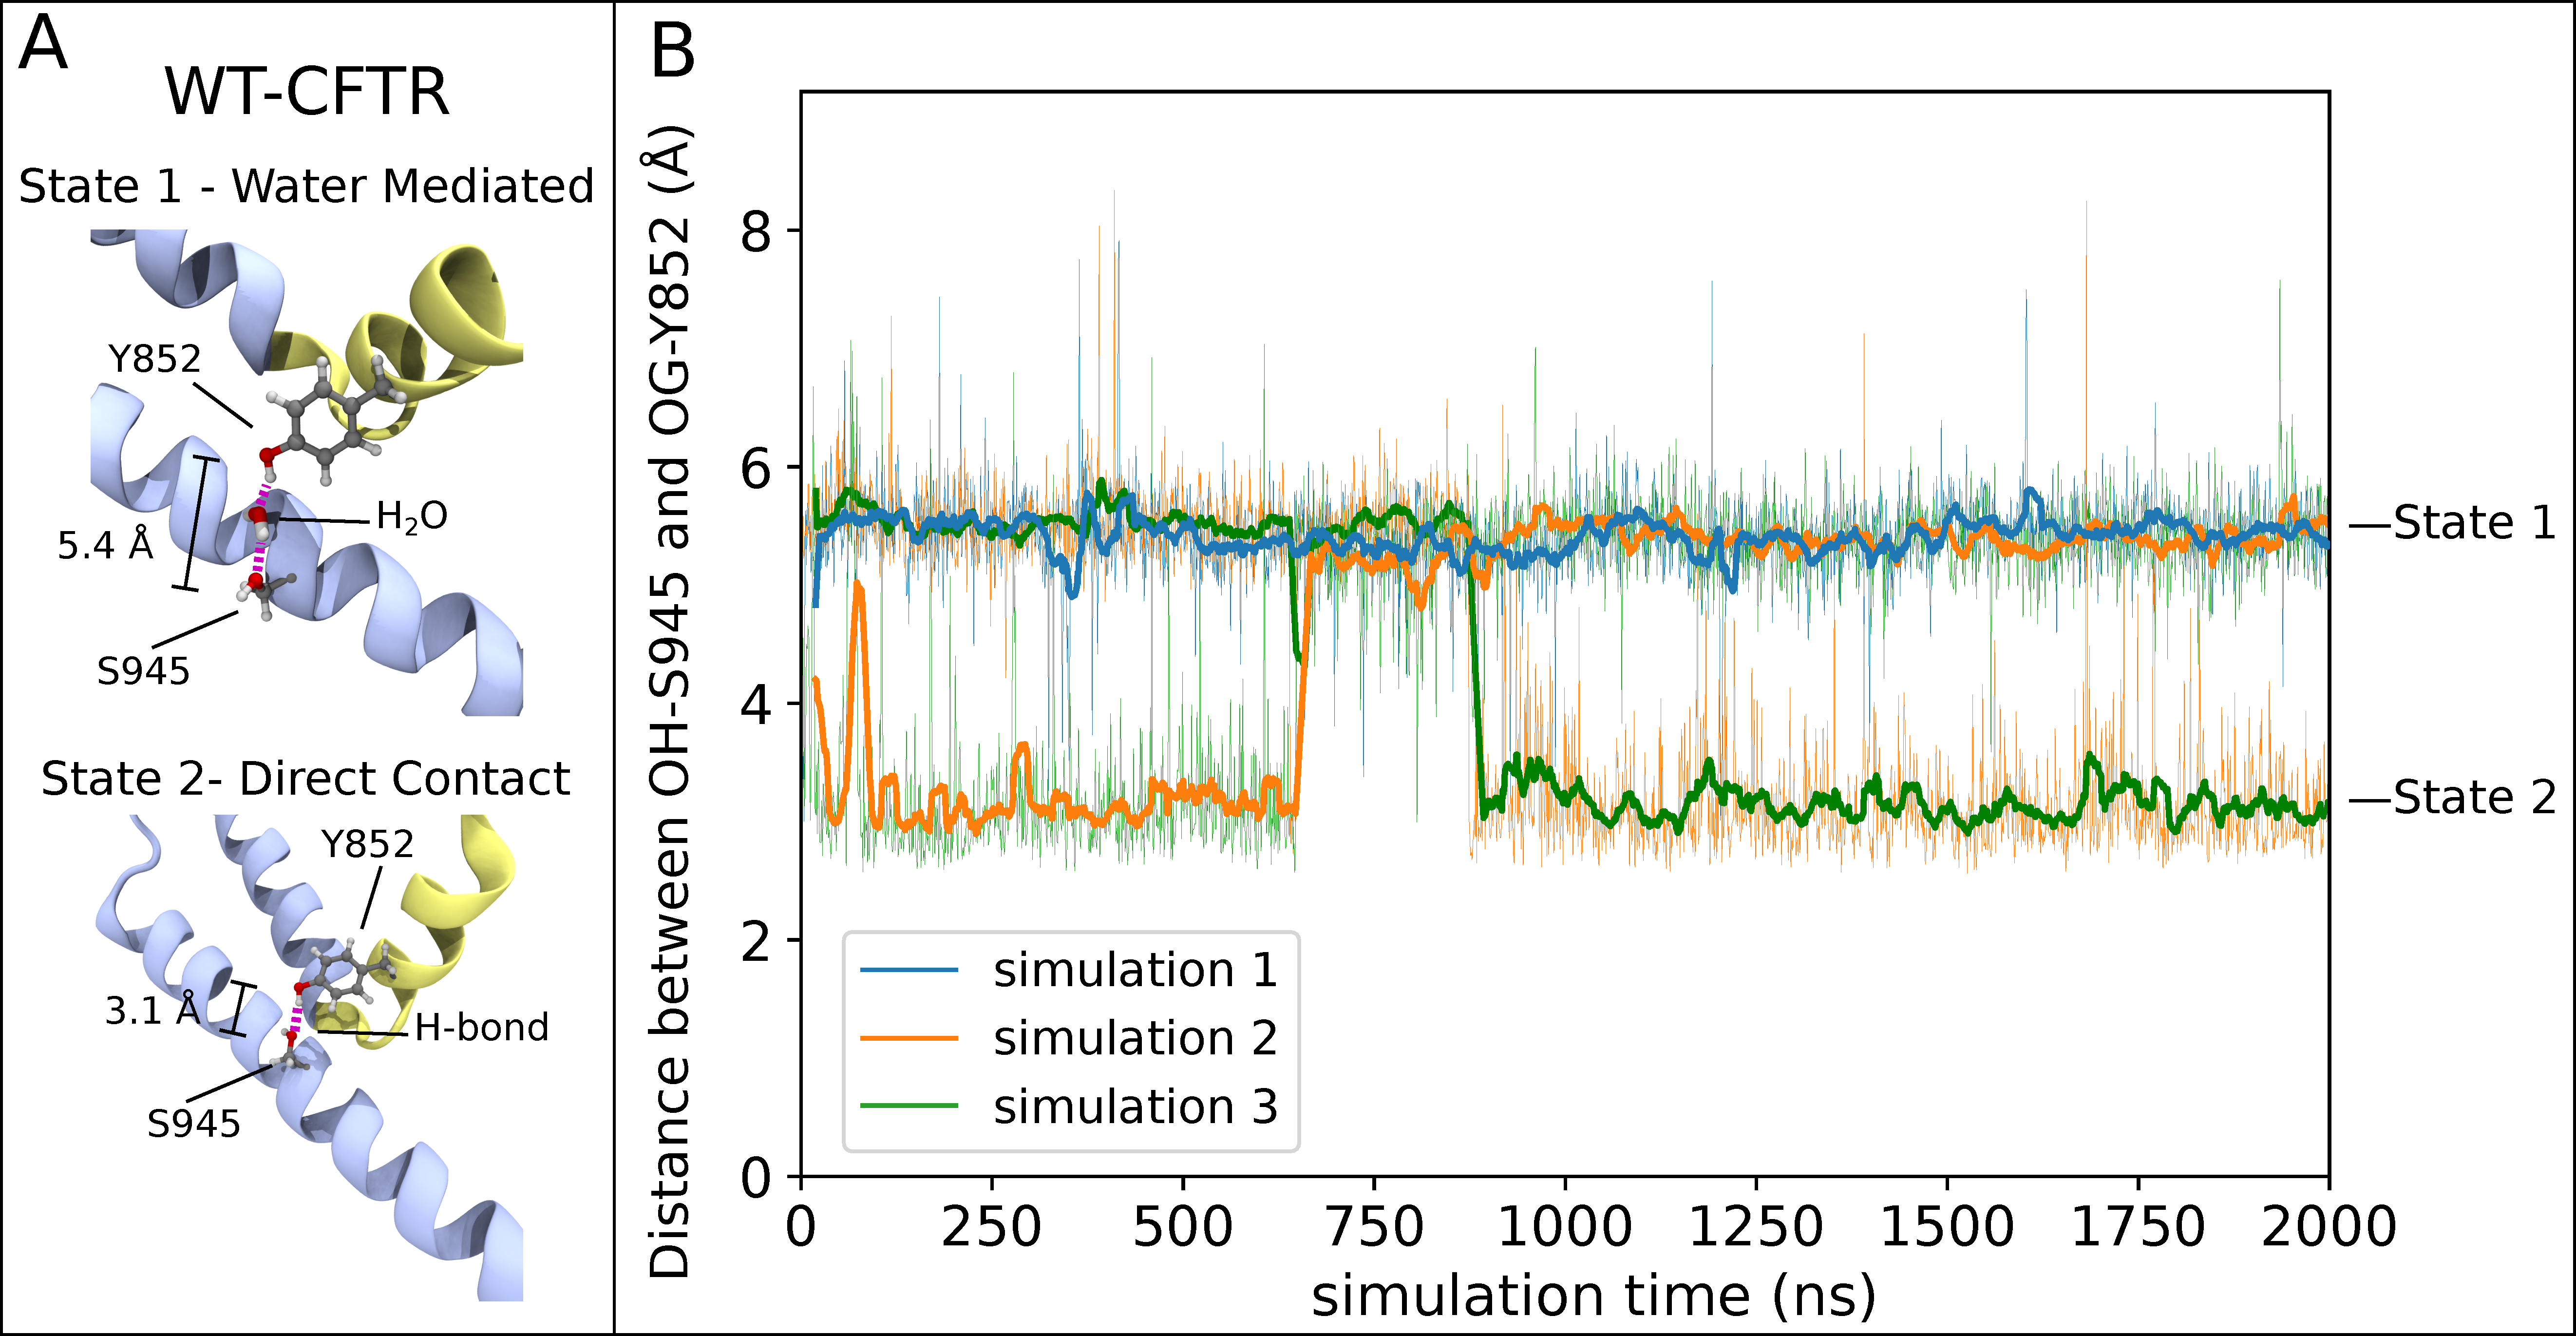
\includegraphics[width=\textwidth]{figures/S945L/supp1_MD.pdf}
\end{center}
	\captionsetup{singlelinecheck = false, justification=raggedright}
\begingroup
\captionof{figure}[Detailed View of the Hydrogen Bond Netowrk in WT-CFTR] {\textbf{Detailed View of the Hydrogen Bond Netowrk in WT-CFTR}}{A. In our simulations we observe two possible states. State 1 occurs when a water molecule stably mediates the interaction between the sidechains of S945 and Y952. State 2 occurs when they are in direct contact with each other. B. The distance between the oxygen atoms in the polar side chains of S945 and Y852 throughout the WT simulations. In simulation 1 the system remains in state 1 throughout. Simulation 2 begins in state 1 but transitions to state 2 at 900 ns. Simulation 3 begins in state 2 but transitions to state 1 at 700 ns. Data is graphed with a 20 ns moving average to more clearly delineate the difference between the two states. This data indicates that the two states each contribute to the stable hydrogen bond network between Y852 and S945.}
\label{S945L_MD_S1}
\endgroup

\begin{center}
	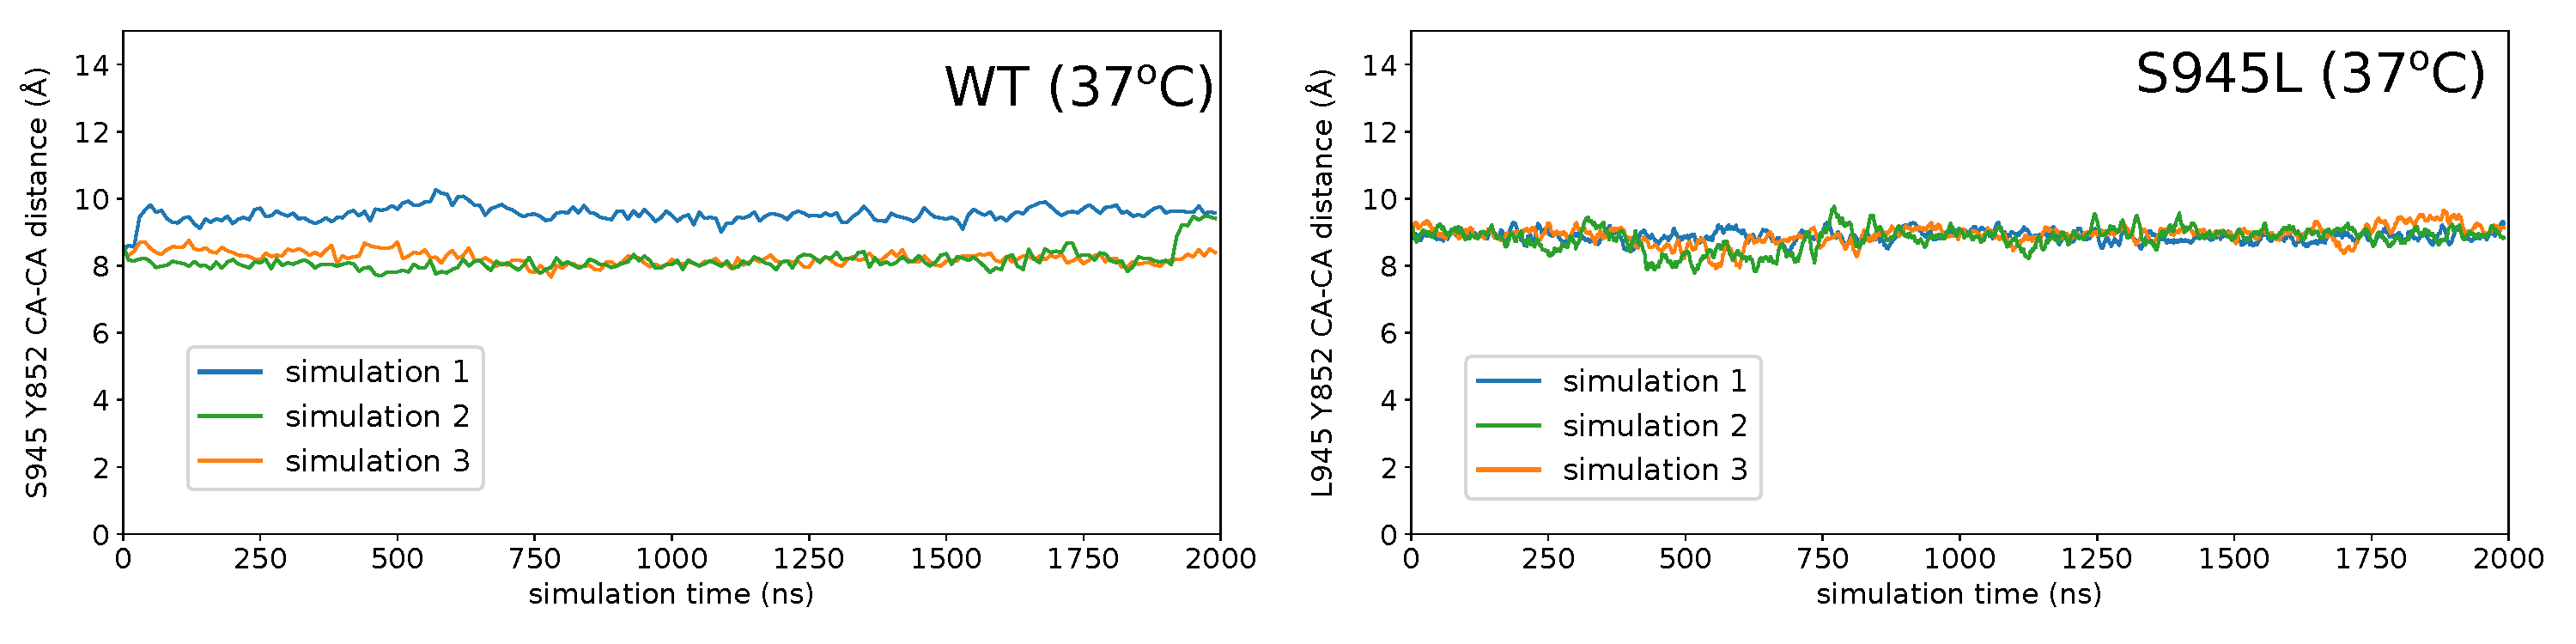
\includegraphics[width=\textwidth]{figures/S945L/310K_supp.pdf}
\end{center}
\captionsetup{singlelinecheck = false, justification=raggedright}
\begingroup
\captionof{figure}[Simulations of WT-CFTR and S945L-CFTR at Physiological Temperature] {\textbf{Simulations of Both WT-CFTR and S945L-CFTR at Physiological Temperature ($37^o$C)}}{In the WT data, we again see a stable interaction between Y852 and S945. The simulations 2 and 3 remain in state 2 throughout the whole simulation, with simulation 2 changing to state 1 at roughly 1900 ns. Simulation 1 quickly transitions to state 1 and remains there throughout the simulation. In S945L, the presence of the lipid bilayer has slowed down the kind of conformational changes we would expect from a mutation like S945L. Unfortunately, no pathogenic motions were visible at physiological temperatures on the timescales accessible with unbiased MD simulations. The Y852 and L945 amino acids remained at a distance somewhere between state 1 and state 2. These results motivated a more rigorous study with umbrella sampling in order to understand the molecular details of the defect which the S945L mutation causes to CFTR. }
\label{S945L_MD_S2}
\endgroup

\begin{center}
	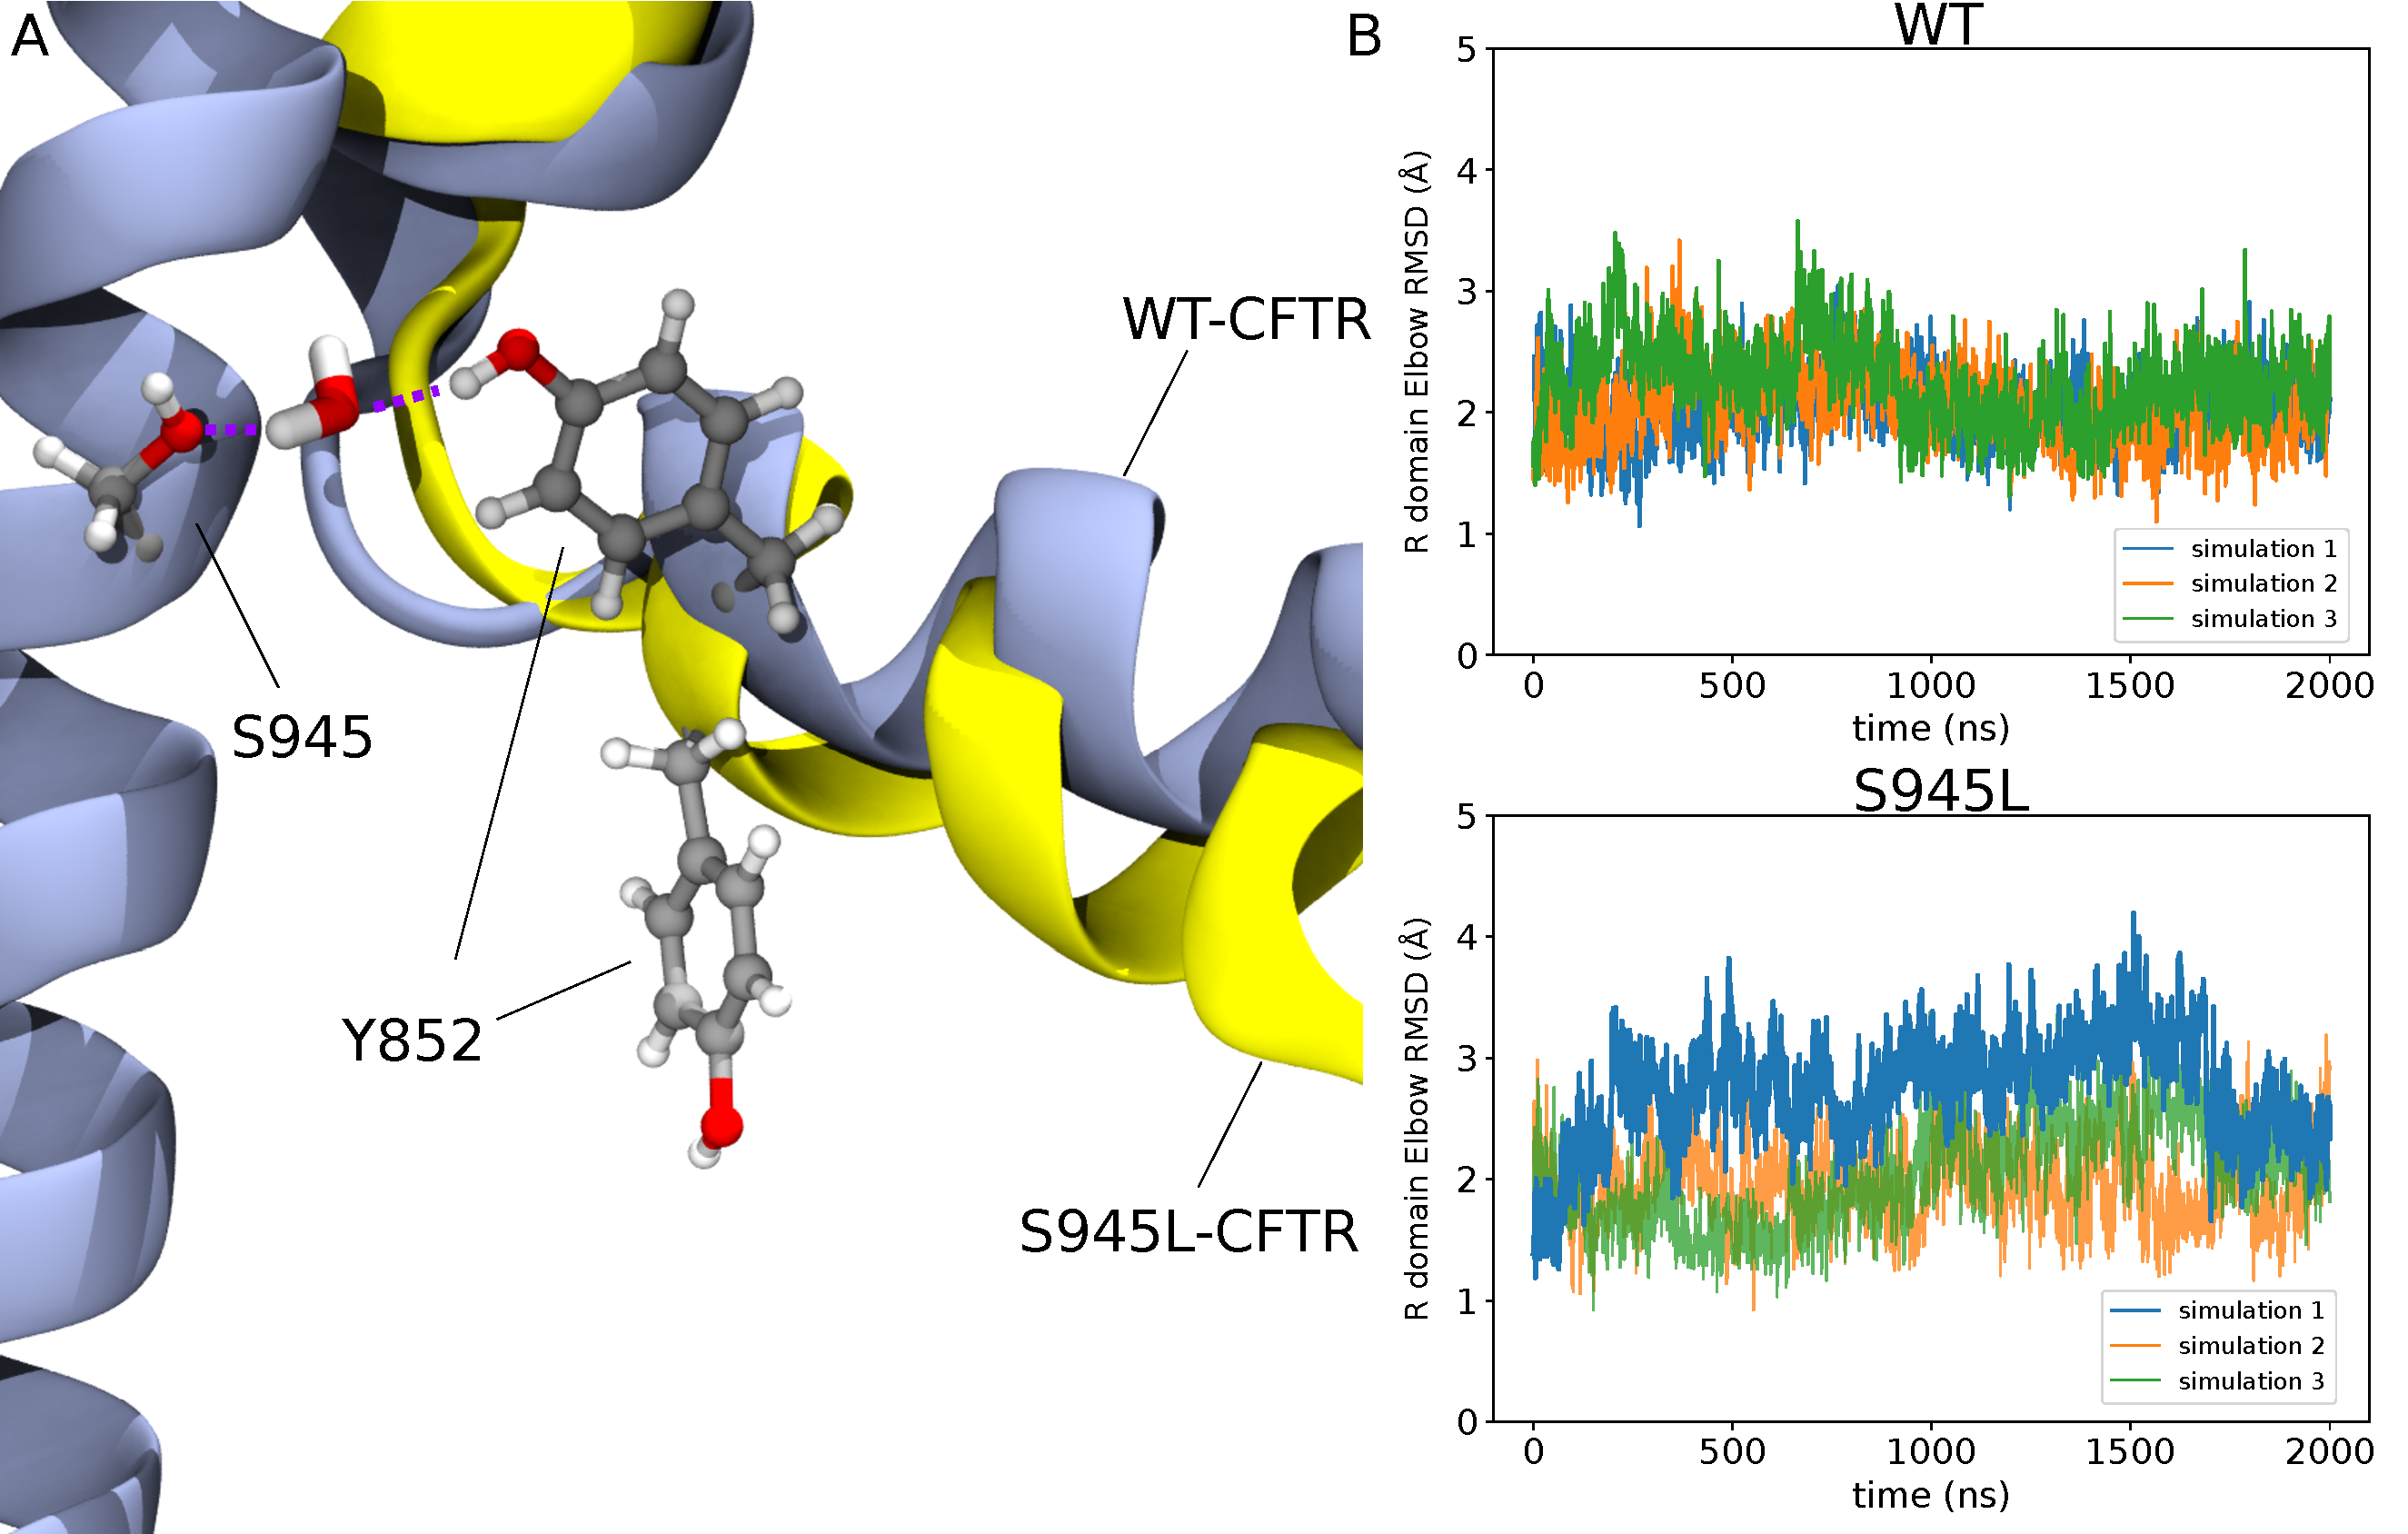
\includegraphics[width=\textwidth]{figures/S945L/supp3_MD.pdf}
\end{center}
\begingroup
\captionsetup{singlelinecheck = false, justification=raggedright}
\captionof{figure}[Local Conformational Change of the Elbow Between TM8 and the R-domain. ] {\textbf{The Local Conformational Change of the Elbow Between TM8 and the R-domain.}}{(WT-purple, S945L-yellow) A. The Y852 side chain sits in the elbow of the R-domain (amino acids 845-886) and when it is perturbed, a shift in the elbow is observed. This conformational change is proposed to influence the gating cycle of CFTR. B. The Root Mean Squared Deviation (RMSD) values of the elbow region, calculated with reference to the alpha Carbon Atoms of the 6MSM structure. Simulation 1 was the replicate with the greatest perturbation compared to the WT structure in the unbiased simulations (Figure \ref{S945L_MD_1}B). The data for simulation 1 of the S945L mutation indicates a destabilisation of this elbow region. This is proposed to cause defects with both the gating cycle of the protein and the stability of the correctly folded state.}

\label{S945L_MD_S3}
\endgroup


\section{Method Details}
\subsection{Molecular Dynamics}
2.1 Molecular Dynamics
The CFTR protein model used for molecular dynamics simulations was based on the ATP-bound human CFTR cryogenic electron microscopy (cryo-EM) structure (PDB ID: 6MSM) \cite{zhang2018}. The construction of the CFTR protein system, including the modelled part of the R domain, has been described previously \cite{wong2022}. In brief, the CFTR model was embedded in a simplified cell membrane model containing pure 1-palmitoyl-2-oleoyl-sn-glycero-3-phosphocholine (POPC) lipids then solvated with 150 mM KCl on both the cytoplasmic and periplasmic sides.

In this study, the software Gromacs v2021.1 \cite{abraham2015} was used for all MD simulations. Molecular mechanics parameters were supplied via the CHARMM36m \cite{huang2016} force field with the following modifications for faster simulation performance: virtual site topologies \cite{feenstra1999} for all molecules while using MkVsite36 to generate topologies for the ATP molecules \cite{larsson2020}, as well as parameter adjustments specific to lipids \cite{olesen2018}. The initial positions of all molecules were equilibrated for production runs in two phases: first via energy minimisation using a steepest descent algorithm, then followed by a 6 ns simulation where position restraints were imposed on all non-hydrogen atoms and then gradually relaxed. 

A series of 2 $\mu$s Production MD simulations were carried out with three replicates for each of WT and S945L-CFTR. To decrease computational expense, elevated temperatures of 350 K were used (77°C) to accelerate conformational transitions. The use of elevated temperatures to study defects in mutant CFTR was validated previously \cite{wong2022}. All measurements of Root Mean Squared Deviation (RMSD) were calculated using the positions of alpha carbons in the 6MSM PDB structure 8 as a reference. 

\subsection{Umbrella Sampling Protocols}
The free energy surfaces were constructed by measuring the potential of mean force (PMF) profile between the amino acids Y852 and S/L945. The distance between the alpha carbon atoms in these amino acids was used as the collective variable for the calculation. This distance was varied from 6-16 $\mbox{\angs}$ with a restraint of 10 kcal/mol/$\mbox{\angs}^2$. Umbrella sampling simulations were performed in 10 windows spaced 1 $\mbox{\angs}$ apart. After 100 ns of equilibration for each window, 100 ns of data were collected. The resultant PMF profiles were calculated from the average of the 5 profiles determined from 5 independent samples of 20 ns each. Uncertainties for this result were calculated as twice the standard error of the mean for these 5 samples. The calculations have clearly converged, demonstrated by uncertainties of less than 1 kcal/mol in the free energy surfaces of both the WT and S945L-CFTR. Plumed 2.6 \cite{bonomi2009, tribello2014, bonomi2019} was used to perform the umbrella sampling, and WHAM \cite{grossfield2012} was used to calculate the PMF profiles. 

\chapter{Resolving a Conducting Conformation of CFTR Using Free Energy Calculations}
\label{chap:opening}
\setcounter{figure}{0}
\renewcommand{\thefigure}{\arabic{chapter}.\arabic{figure}}
\begin{chapquote}{ Zachary Picker. Layperson. (personal communication)}
You wanna fight? 
\end{chapquote}


\section*{\centering Abstract} 
The misfunction of the CFTR gene causes Cystic Fibrosis. The protein must form an ion channel to conduct both chloride and bicarbonate in order to avoid disease. The recent development of small molecules known as potentiators has demonstrated the clinical efficacy of modulating the mutant forms of the protein such that it occupies an conducting conformation to relieve disease symptoms. Hence, determining the precise mechanism behind ion conduction through CFTR has important implications for ongoing drug discovery efforts.

Existing atomic structures of CFTR leave unresolved questions behind this conduction mechanism, since these structures exhibit constrictions smaller than the ions themselves. This indicates that there must be some conformational changes to this structure for ions to pass through CFTR. Here we present innovative simulation techniques which combine unbiased molecular dynamics, principal component analysis, OPES-Metadynamics and umbrella sampling to study the conduction of both chloride and bicarbonate through the selectivity filter of human CFTR. We also used this model to study the R334W disease causing mutation and confirm it as a conductance defect. 

Our proposed open structure is in better agreement with both theoretical predictions and experimental measurements of the pore architecture of CFTR. We also propose electrophysiology experiments to experimentally test whether this conformation is correct. The discovery of an open structure of CFTR has important implications for ongoing drug discovery efforts.

Even the limited success of this study demonstrates that computational power and protein forcefields are now sufficiently developed to take advantage of the large database of protein structures collected through the cryo-EM ``resolution revolution'' and AI based protein structure predictions. In this era of structural abundance, MD based methods can now be used to elucidate even more of the protein conformational landscape. This signals an exciting future for computational structural biology and biophysics.

\section{Introduction}

Ion channels are crucial to many cellular functions. When they misfunction, they may cause pain or disease \cite{kingwell2019, kim2014}. Hence, they have been pursued as targets for drugs, and the molecular basis for their conduction of ions has been studied closely for some time \cite{santos2017, doyle1998, roux1993}.

One of the most well-known ``channelopathies'' is caused by loss-of function mutations in an anion channel, the Cystic Fibrosis Transmembrane conductance Regulator (CFTR). This misfunction leads to Cystic Fibrosis (CF) \cite{riordan1989,gadsby2006}. This is a fatal genetic condition which afflicts an estimated 162000 people worldwide, with a significant number of people unable to access treatment \cite{guo2022}.

The function of mutant CFTR can be restored by molecules known as CFTR modulators. A kind of CFTR modulator known as potentiators interact directly with CFTR to cause it to favor its open, conducting conformation \cite{liu2019}. In currently available cryo-EM structures of CFTR, there is a constriction along the ion conduction pathway which is too small to allow the ions to pass \cite{zhang2018} (Figure \ref{constricted_sel_filter}A). Hence, the full conduction pathway of ions through CFTR is not yet understood. To understand how these drugs work and to improve on them, a molecular-level understanding of the ion conduction through CFTR is critical.

The ion permeation pathway of CFTR can be split into two sections. The inner vestibule and the selectivity filter. We have previously studied the motion of chloride through the inner vestibule in chapter \ref{chap:R352Q} \cite{wong2022a}, and in this chapter we will study conduction through the selectivity filter.

The selectivity filter can also be divided into two parts. A lower ``conductivity selectivity filter'' and a higher ``permeability filter'' (Figure \ref{constricted_sel_filter}B). The different sections in the selectivity filter were characterised by measuring the permeation profiles of different anions under different mutations and the rate of modification by reagents \cite{elhiani2010, linsdell2016}. 

The lower ``conductivity selectivity filter'' appears to bind anions as they move through the channel while the ``permeability selectivity filter'' is narrow and hydrophobic, so anions are partially dehydrated as they move through. This latter section is thought to be the origin of the lyotropic sequence of anion selectivity through the channel (Figure \ref{constricted_sel_filter}B) \cite{linsdell2021}. 

\begin{figure}
	\begin{center}
		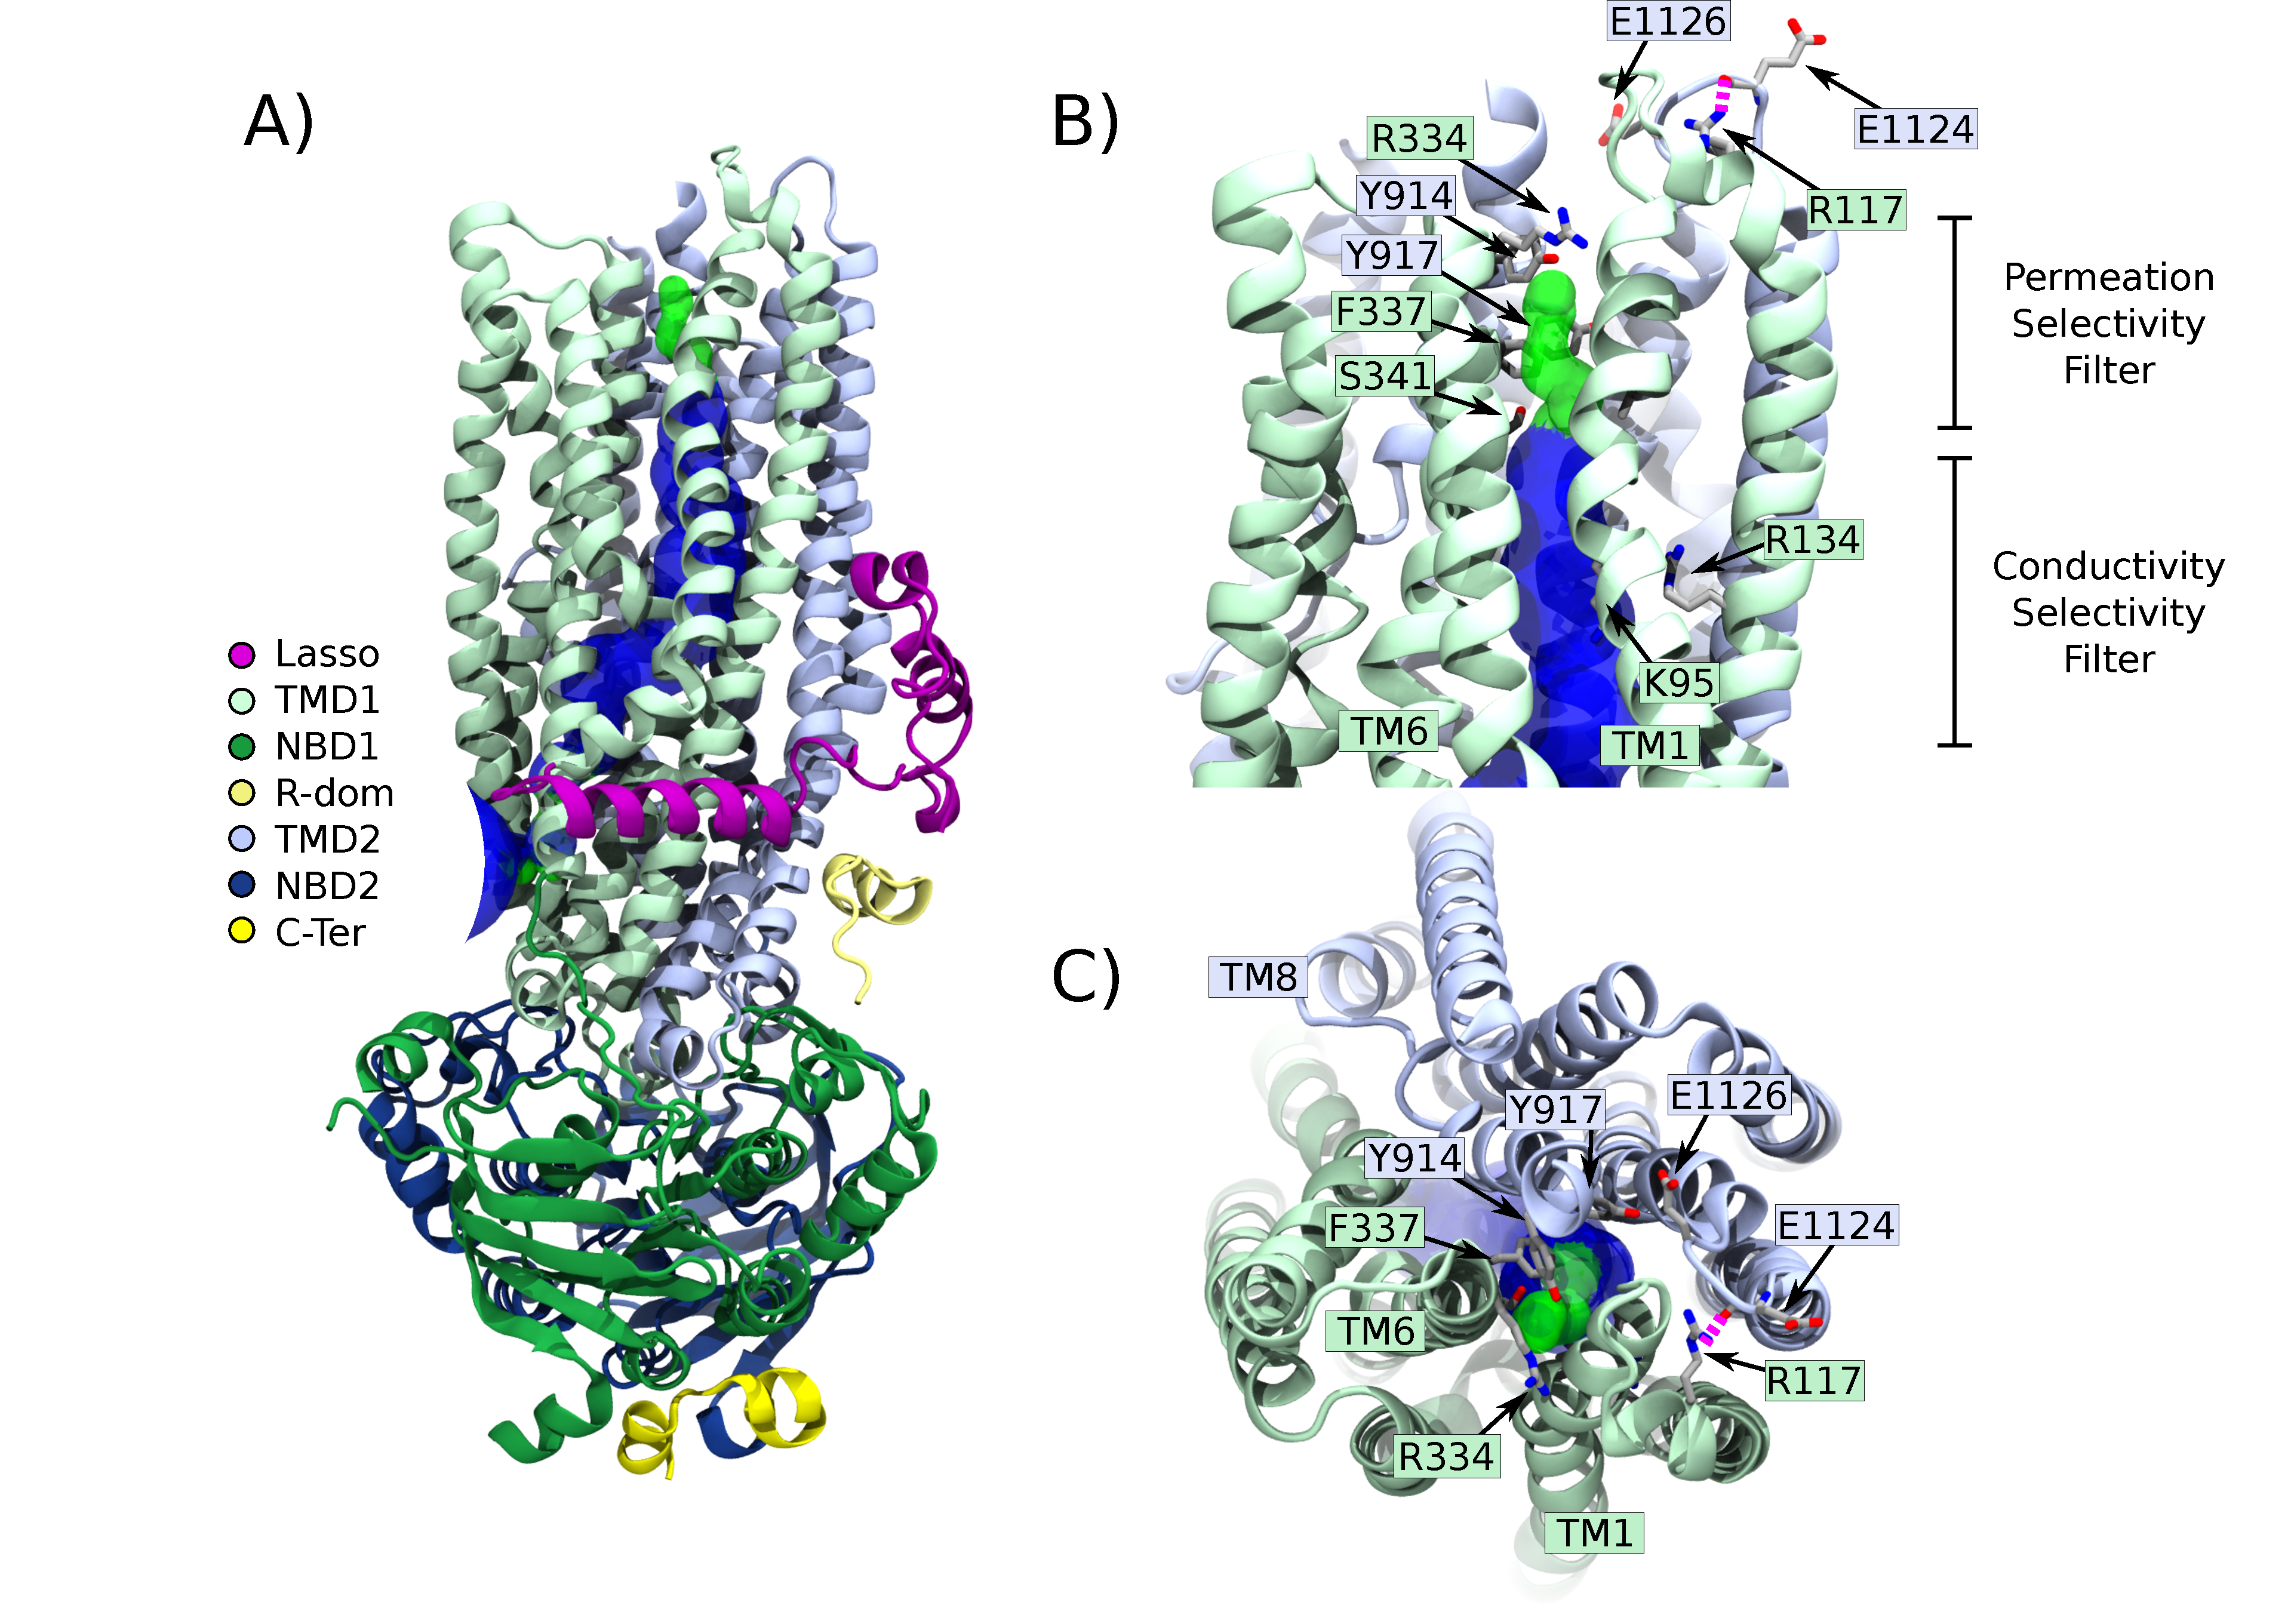
\includegraphics[width=1\textwidth]{figures/opening/overall_hole_constricted.pdf}
	\end{center}
	\captionsetup{singlelinecheck = false, justification=raggedright}
	\caption[Constriction in Cryo-EM Structure (6MSM)] {\textbf{Constriction in Cryo-EM Structure (6MSM)}}{The most recent experimentally resolved structures of hCFTR bound to ATP has a constriction smaller than the radius of chloride ions \cite{zhang2018}. The purpose of this study is to discover a dilated, conducting conformation of CFTR by using this cryo-EM structure as a starting point. A) The constriction occurs between TM1 and TM6 on TMD1. The space filling probe is colored blue when a hydrated ion may pass, while it turns green when the ion must be dehydrated. The probe truncates when it encounters a constriction smaller than an ion. B) Close up of the constriction. Observe how the constriction begins at S341 in the permeability filter and ends at R334 where there is no available space to pass. This leads us to believe that movements in TM6 will help the channel to open. C) A top down view of the selectivity filter. Observe how the architecture of TM1 and TM6 have resulted in a constriction around the conduction pathway.}
	\label{constricted_sel_filter}
\end{figure}

%Due to the importance of the conductance of this channel in disease pathology, a molecular understanding behind the basis of its conductivity will inform future efforts in drug design and improve patient outcomes. Unfortunately, current structures of CFTR are insufficiently dilated in order to conduct anions \cite{zhang2018, liu2019, fiedorczuk2022}. (Figure \ref{constricted_sel_filter}C).

The motion of chloride through the selectivity filter has been studied in two other \textit{in silico} studies to date \cite{farkas2020, zeng2021}. In the first computational study, performed on zebrafish CFTR (PDB ID: 5W81) \cite{zhang2017a}, metadynamics was used to push chloride around the CFTR selectivity filter, to resolve the conduction pathway. The path the authors discovered appears to agree with \textit{in vitro} studies of the selectivity filter in human CFTR \cite{linsdell2016}. However, these MetaD calculations found a significant energy barrier to the passage of chloride (roughly 10 kcal/mol) \cite{farkas2020}. This sizeable energetic barrier conflicts with experimental measurements of the channel's conductivity, and indicates that the tested protein conformation is not sufficiently open to readily conduct ions. 

In the second study, hCFTR was studied with a strong applied electric field in MD simulations \cite{zeng2021}. These authors were able to observe the permeation of chloride ions through the channel. However, the number of conduction events these authors observed would imply a conductivity of 0.54 pS (17 events in 10 $\mu$s of sampling at a substantial 500 mV bias). This conductivity is an order of magnitude below the experimentally measured conductivity of CFTR (6-10 pS) \cite{gong2004, lee2007, linsdell2001, sheppard1999}. These two studies indicate that there are conformational states of CFTR, not yet experimentally visualised, which will support the conduction of chloride and other anions. 

These prior MD studies have focussed on the conduction of chloride, since it is the most physiologically important species to permeate through CFTR. However, it is actually one of the smallest ions which can pass through CFTR. Larger ions such as bicarbonate and glutathione also move through the channel and their failure to do so plays an important role in disease pathology \cite{gao1999, kogan2003, linsdell1998, tang2009, larusch2014, jun2016}. Hence, it is clear that there is a need to move beyond the available cryo-EM structures of CFTR, to find a conducting conformation which can support the passage of larger anions as well as chloride. 

An \textit{in silico} attempt to resolve this issue has been made previously by constructing a model based on zCFTR (PDB ID: 5W81 \cite{zhang2017a}) and steering it toward the outward facing conformation of a distantly related ABC transporter, SAV1866 \cite{hoffmann2018, dawson2006}. However, this resulted in a conformation with a very different architecture to what would be expected from experiments, and so it is difficult to draw testable predictions from the resulting model \cite{hoffmann2018, linsdell2018}. The pore architecture of CFTR has consequences for its function so it must be investigated carefully \cite{linsdell2016, linsdell2018, cui2008}. 

The helices which form the selectivity filter and their associated extracellular loops have been shown to exhibit considerable flexibility. These features play an important role in the selectivity of ions and gating kinetics \cite{linsdell1998, kim2019, negoda2018, negoda2019}. In particular, a recently performed electrophysiology study demonstrated altered gating kinetics in the R117H mutation. Previously, it was thought that R117 forms a salt bridge with E1126 \cite{cui2014}. But more recently, experiments by Simon and Csnady demonstrated that it is E1124 which makes a contact to R117, by interacting with the carboxyl oxygen atom in the backbone of R117, not E1126 \cite{simon2021}. This interaction is visible in available cryo-EM structures of hCFTR (Figure \ref{constricted_sel_filter}B). 

These \textit{in vitro} results correspond well to the implications of our presented \textit{in silico} study. The current state of the literature leaves the role of E1126 in channel gating unresolved, but through our MD experiments we will show how in the conducting conformation of CFTR, E1126 appears to form a salt bridge with R334. We will also propose a test of this hypothesis through patch-clamp electrophysiology experiments. 

Resolving the conduction mechanism of ion channels has been of keen interests to the computational biophysicists for some time \cite{black2020, flood2019}. To our knowledge, this is one of the first studies to resolve the conducting conformation of an ion channel without a target conformation in mind. 

Hence, the work in this chapter differs in an important way from existing computational studies of ion channels. Many previous attempts to induce conformational changes have been \textit{targeted}---that is, they have usually sought to resolve the energy landscape \textit{between} experimentally determined structural conformations of the protein \cite{hoffmann2018, lev2020, bergh2021, mccomas2022}. However, since there is not yet an experimentally determined structure of CFTR in a conducting conformation, the presented study is instead \textit{untargeted}. 

By combining subtle hints from \textit{in vitro} biophysical experiments on CFTR with results from our MD simulations, we have been able to resolve and study a conducting conformation of the anion channel with the use of multiple ions. This signals how computational methods have become sufficiently developed to use experimentally obtained structural snapshots as starting points, to then explore the local conformational neighbourhood. This approach has the potential to discover new molecular mechanisms within cells.

\section{Results}

\subsection{Long Simulations Reveal Motions Which Dilate the CFTR Pore}
Four independent replicates of unbiased MD were run to simulate WT-CFTR. Each replicate was used to generate a trajectory which was at least 2 $\mu s$ long. This gave a combined 8.2 $\mu$s of sampling. 

Choosing CVs from these unbiased statistics is not trivial. In post processing, the motions of the transmembrane helices were analysed using Principal Component Analysis \cite{pearson1901, hotelling1936} (Figure \ref{PCA_motions}A). 

The first two Principal Components represented 38\% of the kinetic variance in the unbiased data. Additionally, they captured motions in TM1 and TM6 in motions which dilated the extracellular pore in a location we expected from experiments (Figure \ref{PCA_motions} B-C) \cite{linsdell2018, negoda2018, negoda2019}. These factors validated their choice as collective variables in our enhanced sampling calculations.  

The amino acids analysed with PCA were chosen carefully (Table \ref{red_alpha_carbons_table}). Amino acids in disordered loops were excluded from analysis as they make large motions quickly. Large, fast motions were excluded because they would otherwise distort the optimal slow degrees of freedom which we hope to investigate with free energy calculations \cite{noe2001}. A more detailed discussion of our choice in CVs can be found in section \ref{supp_cv_choice}.

	\begin{center}
		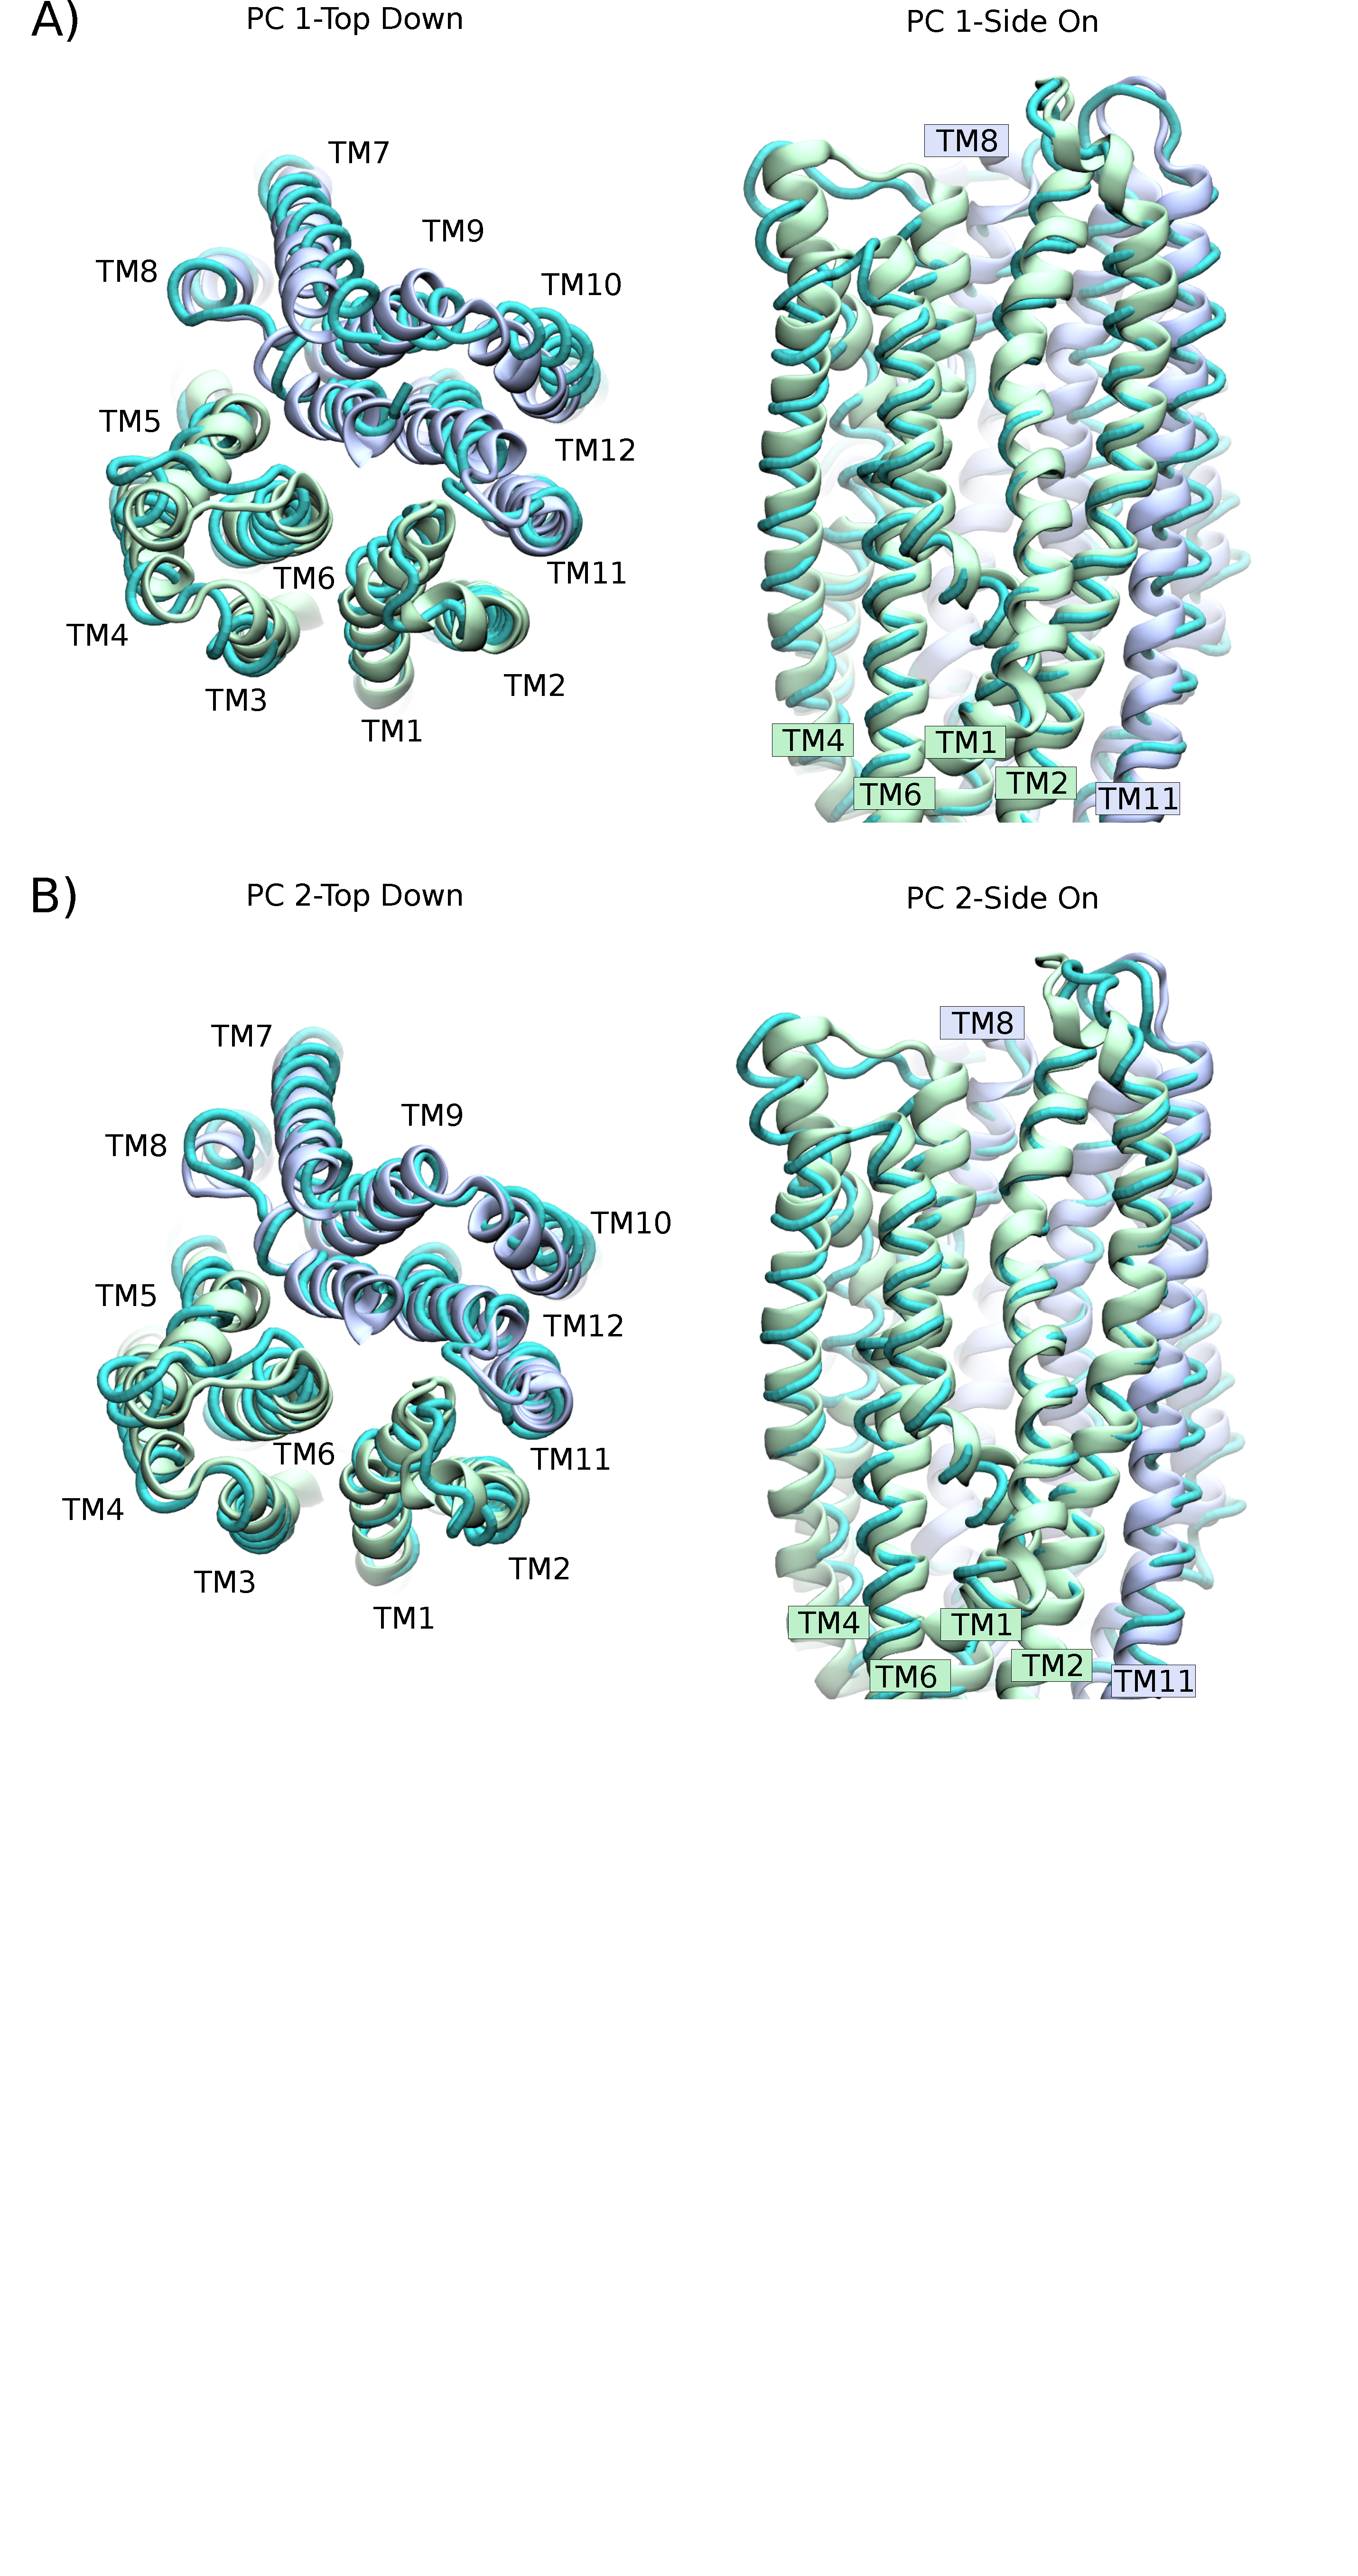
\includegraphics[width=1\textwidth]{figures/opening/pca_motions.pdf}
	\end{center}
	\begingroup
	\captionsetup{singlelinecheck = false, justification=raggedright}
	\captionof{figure}[Principal Component Analysis Reveals Large Motions in CFTR Transmembrane Helices] {\textbf{Principal Component Analysis Reveals Large Motions in CFTR Transmembrane Helices}}{A) Visualisation of the results from principal component analysis from 4 independent simulations, comprising 8.2 $\mu s$ of unbiased MD sampling. Motions along the first two principal component vectors were found to capture 38\% of the variation in the data set and were used in further analysis. B) Visualisation of the first principal component vector (PC1). Note the motion in TMs 1, 6 and 8 C) Visualisation of the second principal component vector (PC2). Note the motions in TMs 1 and 6 but in directions orthogonal to PC1. A video has been rendered of the motions associated with PC1 and PC2 and can be accessed at the following \href{https://zenodo.org/record/7036443#.Yw7CZNJBwUE}{link}.\footnote{\href{https://zenodo.org/record/7036443\#.Yw7CZNJBwUEi}{https://zenodo.org/record/7036443\#.Yw7CZNJBwUEi}} D) Visualisation of the dilated open state which we will analyse in detail in subsequent sections. This structure was obtained by a linear combination of PC 1 and 2 followed by unbiased MD simulations. } 
	\label{PCA_motions}
	\endgroup

	Because the more atoms we included in our collective variables, the slower our calculations would run, we limited subsequent free energy calculations to consider a set of helices which directly surrounded the pore (Table \ref{red_alpha_carbons_table} Figure \ref{steer_cas_fig}). The same technique was employed in \cite{hoffmann2018}. In the next section, we will show how we combined these two PC motions with OPES-MetaD to discover a dilated conformation of the CFTR pore (Figure \ref{PCA_motions}D). 

\subsection{OPES-Metadynamics Finds a Stable Conformation with an Open Extracellular Pore}

The principal components identified in the previous section were used as collective variables to study the motion of the pore lining transmembrane helices in WT-CFTR. A two dimensional Free Energy Surface along these CVs was constructed through the use of 8 independent walkers, each running for $1.5~\mu$s with On the Fly Probability Enhanced Sampling-MetaDynamics (OPES-MetaD), using a barrier parameter of 38.2 kcal/mol (\ref{summary_FES}A). Convergence of these calculations is demonstrated in Figures \ref{convergence_opes_1}-\ref{convergence_3}. 

Note the presence of a local free energy minima at (0.010, 0.021) in Figure \ref{summary_FES}A. When this coordinate in CV space was investigated closely, we noticed that the extracellular pore had dilated significantly (Figure \ref{summary_FES}B). Further, this dilated configuration was stable in 3 replicates of unbiased MD on timescales of 500 ns (Figure \ref{summary_FES}C). 

This dilated structure has a pore architecture where the narrowest constriction was 2.8 $\angs$ (Figure \ref{summary_FES}C). This larger opening completely removed the aberrant constriction seen in the cryo-EM structure, and the dilation occurred where we expected, between TM1 and TM6 (Figure \ref{summary_FES}D). Continuum models have previously estimated the constriction in CFTR to be 2.4 $\angs$ \cite{jun2016}, which is close to our own estimate. 

	\begin{center}
		\includegraphics[width=1\textwidth]{figures/opening/summary_dilated_structure_1.pdf}
	\end{center}
	\begingroup
	\captionsetup{singlelinecheck = false, justification=raggedright}
	\captionof{figure}[Free Energy Calculations Discover a Dilated Conformation of CFTR.] {\textbf{Free Energy Calculations Discover a Dilated, Conformation of CFTR.}}{A) The free energy landscape obtained along PC1 and PC2 through OPES-Metadynamics. Note the free energy minimum corresponding to a collapsed structure found via cryo-EM in the bottom left, and the free energy minimum at (0.010,0.021). This latter well was found to correspond to a stable, open structure which appears capable of passing anions. B) A visual comparison between the constricted structure and our dilated open structure. Note how the extracellular opening is much wider in the dilated structure. The R334 and E1126 amino acids are visualised to show how they come into contact with each other in the dilated structure. C) A quantitative measurement of the pore radius for different conformations of CFTR, generated with HOLE2 \cite{smart1996}. Dehydrated chloride has a radius of 1.7 $\angs$, while the collapsed cryo-EM structure of hCFTR exhibits a constriction of 1.2 $\angs$. Hence, even if chloride were to be dehydrated during its migration through the selectivity filter, there would need to be some change to the conformation of the selectivity filter. By contrast, our proposed dilated open structure exhibits a constriction of 2.8 $\angs$ at its  narrowest point. This pore profile was generated from a snapshot obtained after 500 ns of unbiased MD. Indicating that this open structure is energetically stable.  D) A side on comparison between the collapsed cryo-EM structure and the dilated open structure. The green constriction denotes the region too small to pass ions. This constriction has been completely removed in the dilated structure we have discovered. }
	\label{summary_FES}
	\endgroup


\subsection{The Open Conformation is Stabilised by the R334-E1126 Salt Bridge}
\label{salt_bridge}

To search for interactions which might be stabilising the dilated structure, giving rise to the free energy minimum in Figure \ref{summary_FES}A, we inspected pairs of positive and negative amino acids. This led us to the discovery of a novel salt bridge linking R334 and E1126. This salt bridge could only form in the dilated conformation, due to the movements of TM1, TM6 and TM8. It could not form in the collapsed cryo-EM structure (Figure \ref{salt_bridge_fig}A). 

%The movements of TM1, TM6 and TM8 allowed E1126 on ECL5 to come closer to R334 on TM6. We expect this new salt bridge to be an important factor in stabilising the conducting conformation of CFTR.  

The link between these amino acids was found to be stable in 3$\times$500ns unbiased MD simulations of the dilated structure. While it did not form at all in simulations of the cryo-EM structure (Figure \ref{salt_bridge_fig}B).

This is a novel interaction within CFTR which we have discovered through the use of simulations. Suggestions that this salt bridge exists can be found in the literature, but it has not been confirmed \cite{cui2014, wang2016, gong2004, zhang2005}. We suspect this was due to the important role that R334 plays in conduction of anions and channel gating. We will discuss the implications of this salt bridge and the means for testing its presence \textit{in vitro} in the Discussion.

\begin{figure}
	\begin{center}
		\includegraphics[width=1\textwidth]{figures/opening/salt_bridge_E1126_R334_figure.pdf}
	\end{center}
	\captionsetup{singlelinecheck = false, justification=raggedright}
	\caption[The Dilated Conformation of CFTR Gives Rise to the R334-E1126 Salt Bridge] {\textbf{The Dilated Conformation of CFTR Gives Rise to the R334-E1126 Salt Bridge}}{A) A comparison between cryo-EM and dilated CFTR structures. In the cryo-EM structure, R334 and E1126 are far apart and do not make contact. In the dilated structure, the transmembrane helices rearrange such that R334 and E1126 make contact. B) In simulations of the cryo-EM structure, the salt bridge is never formed. However, in the dilated structure R334 and E1126 come close together and form a stable salt bridge. The black dotted lines in both plots denotes the distance below which the side chains are in steric contact with each other. We believe that this salt bridge makes a significant energy contribution to the stability of the open channel. }
	\label{salt_bridge_fig}
\end{figure}

\subsection{Proving the Open Conformation is Capable of Ion Conduction with Umbrella Sampling}

In order to test the ability of the dilated structure to the conduct anions, we employed umbrella sampling to calculate the energy landscape of anions as they permeated through the selectivity filter of CFTR. 

The conduction of chloride through WT-CFTR in simulations of the cryo-EM structure was severely inhibited (Figure \ref{US_anions}A). We obtained a sizeable barrier of 9.7 kcal/mol to the passage of chloride, demonstrating that without dilation, this structure will not allow chloride to pass at a rate in agreement with experiments \cite{gong2004}. By contrast, the dilated conformation obtained in the previous section removes steric barriers to the passage of chloride and larger anions (Figure \ref{US_anions}B). In this structure, a considerably smaller barrier of only 2.5 kcal/mol was observed for both chloride and the larger bicarbonate (Figure \ref{US_anions}C). 

This small barrier is closer to what we would expect to be overcome by the -46 mV resting potential of epithelial cells \cite{josephson1979}. Furthermore, the remarkably similar profiles for both bicarbonate and chloride are in agreement with the energy landscape we would expect from a weakly selective channel like CFTR. Indeed, through our umbrella sampling we have calculated energy landscape through the ``permeability selectivity filter'' of CFTR. Deeper in the pore is the ''conductivity selectivity filter'', where we might expect a difference between the two anions. The lower FES in the vicinity of and R134 K95 in Figure \ref{US_anions}C for bicarbonate compared to chloride may indicate tighter binding at this site. This would lead to lower overall conductance of bicarbonate. Unfortunately, there have not been many studies which have measured the effect of mutations on bicarbonate conductance, but studies of other anions would lead us to expect that R134 and K95 play important roles in the conduction of bicarbonate \cite{linsdell2016}. 

	\begin{center}
		\includegraphics[width=0.6\textwidth]{figures/opening/pmf_fig_1_combined.pdf}
	\end{center}
\begingroup

	\captionsetup{singlelinecheck = false, justification=raggedright}
	\captionof{figure}[The Dilated Conformation of CFTR is Capable of Conducting Anions] {\textbf{The Dilated Conformation of CFTR is Capable of Conducting Anions}}{A) A close-up visualisation of the selectivity filter in the collapsed cryo-EM structure. To pass through this structure, the ion must move past a tight constriction formed by F337, Y914 and Y917. B) A visualisation of the selectivity filter in our dilated \textit{in silico} structure. Here, bicarbonate is pictured but the same conformation was used to construct a PMF of chloride as well. The selectivity filter is not as constricted-and R334 makes a salt bridge with E1126. This brings R334 closer to the conduction pathway where it can help coordinate the permeating anion. Steric barriers to the conduction of anions have also been removed C) PMFs of the anions as they pass through the narrowest point in CFTRs permeation pathway. The collapsed cryo-EM structure exhibits a significant barrier to the conduction of chloride, which is inconsistent with experimental measurements. By contrast, the dilated structure appears capable of permeating both chloride and bicarbonate, with a landscape in agreement with the characterisation of the channel found in experiments. }
	\label{US_anions}
	\endgroup



\subsection{The Open Conformation Can be Used to Study Disease Causing Mutations in the Selectivity Filter, such as R334W}


\begin{figure}
	\begin{center}
		\includegraphics[width=0.6\textwidth]{figures/opening/R334W_pmf_combined.pdf}
	\end{center}
	\captionsetup{singlelinecheck = false, justification=raggedright}
	\caption[R334W Inhibits the Conduction of Anions] {\textbf{R334W inhibits the Conduction of Anions}}{A) A visualisation of R334W-CFTR in the dilated conformation. Note how W334 is placed in the outer part of the pore. B) A PMF derived from Umbrella sampling to compare the energetics of the conductance of chloride through R334W-CFTR to WT-CFTR in the dilated conformation. The WT-CFTR curve has been reproduced from the same data in Figure \ref{US_anions}C. The R334W-CFTR PMF exhibits a larger barrier compared to WT-CFTR indicating that the conduction of chloride will be suppressed in this mutation. It is likely that this additional energy barrier has a particularly deleterious effect on the conduction of the channel because it occurs at the narrowest part of the pore. There are no alternate pathways which might help compensate for the mutation, as was the case for R352Q in chapter \ref{chap:R352Q} \cite{wong2022a}.  }
	\label{R334_pmf}
\end{figure}

There are several disease causing mutations which occur at around the selectivity filter of CFTR (such as E116K, R334\{W,Q,L\},R117\{H,C,P\}, I336K, S341P)\cite{cftr2}. Note how these are all clustered around TM1 and TM6. The fact that mutations to these amino acids causes a loss of function is more evidence to suggest TM1 and TM6 form the permeation pathway for anions in hCFTR, in agreement with previous MD and functional studies \cite{zeng2021,farkas2020, linsdell2016, linsdell2018}. 

A molecular understanding of these mutations can aid in the design of new therapeutics, so as an example, we have used our dilated structure to study the extracellular R334W mutation. Patch clamp measurements of R334W-CFTR have found a single channel reduction in current of 60\% compared to WT-CFTR \cite{gong2004}. According to the Nernst-Planck model, this means we expect a larger energy barrier to the conduction of chloride in the mutant compared to WT-CFTR on the order of 0.6 kcal/mol \cite{kuyucak2001}. This is close to differences in barrier height we observed through umbrella sampling which were between 0.7 and 2.5 kcal/mol (Figure \ref{R334_pmf}B). 

\section{Discussion}

The present study differs in an important way from recent \textit{in silico} investigations of large-scale conformational changes in ion channels. These past studies have focussed on recreating intermediate free energy landscapes between \textit{known} endpoints in conformational space \cite{lev2020, bergh2021, moradi2015}. These studies were \textit{targeted}. Such approaches are critical to the development of molecular techniques to help us understand the energetics and kinetics of protein systems. However, these techniques are inherently more limited by the availability of high quality experimental protein structures than \textit{untargeted} methods. So, we regard this \textit{untargeted} study as a proof of concept---to show how computational methods can move beyond the availability of protein structures.

One could regard the differences between \textit{targeted} and \textit{untargeted} MD methods as similar to the development of unsupervised vs. supervised machine learning methods \cite{grus2015}. Each has its own advantages and drawbacks.

%The advantage of untargeted methods is that By using protein structures as a starting point, we can explore the conformational space around a region to understand more about a protein system. This has been made possible by increasing the increasing accuracy of protein forcefields to reproduce structural ensembles \cite{huang2016} and considerable increases to computer power. 

\subsection{The Dilated Structure Is Consistent with Experiments}
It is pleasing that the results from this chapter appear to be consistent with results from \textit{in vitro} biophysical experiments. The movements in TM1, TM6 and TM8, which dominate the PC1 and PC2, were the kind of dilation we expected from biophysical experiments studying CFTR's selectivity filter \cite{negoda2019,linsdell2016}. The dilated structure also matches experiments which studied the binding of a protein partner WNK1 to TMD1 and other studies which looked at the permeation of bicarbonate \cite{jun2016, kim2019}. These studies indicate that movements of TM1 result in a wide open conformation, which facilitates the movement of bicarbonate ions, in agreement with our own discovery.  

Additionally, the similar conductance profiles between bicarbonate and chloride are what we would expect from a weakly selective anion channel like CFTR \cite{linsdell2016}. Recall that the diffusion coefficient of a particle scales inversely with its radius according to the Stokes-Einstein relation \cite{miller1924}. Since chloride is smaller than bicarbonate, we would expect it to permeate more quickly through the channel, even if it passed over the same energy landscape, particularly through the permeability selectivity filter. 

Given that the conductivity ratio in CFTR is $P_{\rm{HCO3}}/P_{\rm{Cl}}=0.25$, we would expect each ion to have a roughly similar free energy profile through the open channel. At the same time, the selectivity filter in our structure still has a constriction of 2.8 $\angs$, while a hydrated chloride ion has a radius of 3.2 $\angs$, so partial dehydration must still take place during anion conduction. Hence, our dilated conformation is still consistent with the experimentally determined lyotropic selectivity sequence found in other CFTR and other anion channels \cite{linsdell2016}. 

Cysteine cross-linking has been performed on many pairs of amino acids within CFTR \cite{negoda2019, cui2008, negoda2018, wang2012}. Our proposed conducting conformation is in close agreement with these studies, and in some cases, in closer agreement than the available cryo-EM structures. These studies found that the T338C/S1118C and R334C/T1122C cross-links could form in the open state but not in the closed state \cite{wang2012}. In the cryo-EM structure, TM8 stands in the way of these cross links. However, our dilated structure allows unobstructed access between TM6 and TM12, which would allow these cross-links to form. 

With the elucidation of CFTR in a conducting conformation, it may be possible now to design nano bodies or small molecules which select for it \cite{hutter2019}. This would give rise to a new set of tools to understand CFTR's function or even new therapeutics to treat CF. Therapeutics which target the conducting conformation of CFTR will likely be much more effective than current generation potentiators, as it remains unclear whether or not these drugs select for the fully open conformation of CFTR \cite{csanady2019, yeh2017}. 

\subsection{Study Limitations}

We should address the considerable difference in height between the global free energy minimum in Figure \ref{summary_FES}A, which closely corresponds to the cryo-EM structure, and the minimum corresponding to our dilated structure. The dilated structure would appear to have a height of 17 kcal/mol. At first, this difference would seem unphysically high. If these values were correct, the dilated structure would be inaccessible at physiological temperatures. However, we believe this discrepancy is due to limitations of our simulation methods and we have plans to improve them. We believe there are 3 systematic issues which have led to this discrepancy, and outlining these issues will help us improve the study before submission for publication. 

The first and most pressing concern would be to improve our collective variables for OPES-MetaD. The PCA motions outlined in Figure \ref{summary_FES} are likely suboptimal. Note for example how in the dilated structure in Figure \ref{PCA_motions}D, TM1 has moved significantly but this motion is poorly captured by the two motions in Figure \ref{PCA_motions}B-C. Hence, the movement of TM1 is likely in a hidden CV, not captured by PC1 and 2 \cite{bussi2015, bussi2020a}. It is motions like this which have likely led to some hysteresis during the construction of the free energy surface in Figure \ref{summary_FES}A. 

Given that the unbiased simulations of the dilated structure are stable, and they agree with experimental studies, we expect that the dilated state indeed corresponds to a physiologically relevant protein conformation. For the next iteration of this study, we plan to employ more advanced dimensionality reduction techniques such as TICA, VACs and RAVE to make a more careful choice of CVs and gain a clearer picture of the energetics of the fully open state \cite{brotzakis2019, noe2001, schultze2021, brotzakis2019, ribeiro2018}. We expect that the simple reweighing scheme of OPES-MetaD alongside SGOOP optimisation will be of great help in designing optimal CVs \cite{invernizzi2020, invernizzi2022, smith2018, tiwary2016b}. 

The second missing factor from the calculation of this FES is the energetic contributions from the anions, as they pass through the selectivity filter. This is not captured by our CVs. The permeation pathway through CFTR is unusually long, and there has been a demonstrated energetic contribution to the opening transition from the anions anions during channel gating \cite{gong2004, gong2003, gong2003a, tabcharani1993, zhou2002, sorum2015, yeh2015}. 

Finally, we consider the effects of the lipid bilayer which surrounds CFTR. There is emerging interest in the role played by the lipid bilayer in the regulation of CFTR and other membrane proteins \cite{cottrill2020, lin2022, kapoor2021, farinha2018, cui2020, chin2018}. Different bilayer compositions have different physical properties, leading to different behavior by the proteins embedded in them \cite{hickey2011}. In the case of CFTR, many lipid species such as sphingolipids and cholesterol has been shown to lead to different rates of chloride transport, indicating that they play a role in regulating the gating of the channel \cite{aureli2016, farinha2018, cottrill2020}. Hence, it is likely that the zwitterionic POPC membrane used for these simulations struggles to reflect the energetics and kinetics of the membrane surrounding CFTR in its native environment.

The effect of the non-native lipid bilayer composition would also account for the discrepancies we find between our simulations and experiments. Careful biophysical experiments discovered an interaction between the R117 and the carboxyl atom of E1124 \cite{simon2021}. This interaction was not present in our dilated structure, nor was it well preserved in our unbiased simulations of the cryo-EM conformation (data not shown). Similarly, the well characterised R104-E116 interaction is poorly preserved in simulations of the cryo-EM structure and simulations of the dilated structure \cite{cui2014}. This discrepancy is also visible in previous MD studies of CFTR in a non-native lipid environment \cite{zeng2021}. These salt bridges were often broken in our MD simulations, due to interactions between the charged amino acids and the phosphate or choline chemical groups in the phospholipid bilayer. In future we could use newly developed model bilayers of the epithelium to simulate CFTR in a native-like environment \cite{wilson2021}. 

%Given the importance of different lipid species to regulation of CFTR such as cholesterol and sphingolipids, we expect that the zwitterionic POPC lipids used as a model membrane in this study do not fully reflect the native lipid environment of CFTR \cite{farinha2018, cottrill2020}. Recent studies have demonstrated an increasing need to study the bidirectional relationship between membrane composition and membrane protein regulation \cite{lin2022, kapoor2021, cui2020}. Hence, the state of the literature suggests that the salt bridges we mentioned earlier may in fact be regulated by the local environment of lipids around those specific sections of CFTR. 

We regard the above points as room for improvement, and they will be considered carefully in further studies of this dilated structure.

%Mutagenesis studies of the R334 amino acid noticed that many different mutations appear to result in ephys readings which would indicate a loss of function \cite{ge2004, gong2004, linsdell2021}. Surprisingly, the R334W mutation was determined not to alter the relative selectivity between anions in CFTR \cite{sheppard1993}. This is consistent with a wider open pore at the R334 position, as demonstrated in Figure \ref{summary_FES}.



%As shown by the results in the present study, the difficulty in converging a free energy landscape with collective variables derived \textit {ab initio} from long classical MD simulations can be difficult as the CVs are very likely going to be suboptimal. Machine learning techniques, more sophisticated than the simple PCA algorithm used here would likely do a much better job of choosing quickly converging CVs \cite{}. 

%The conformational changes investigated in this study occur within the lipid bilayer. This means that the kinetics and energetics of the transitions we have discovered will be highly dependent on the composition surrounding CFTR. It is well understood that the bilayer composition plays an important role in CFTR regulation and the clinical implications of this are an active area of research \cite{cui2020, cottrill2020}. It would therefore be an interesting study to repeat similar free energy calculations with different bilayer compositions to understand how they might regulate such conformational changes.


\subsection{Proposed Experiments to Test the R334-E1126 Salt Bridge}

The predictions of a stable salt bridge in section \ref{salt_bridge} fill a recent gap in the literature. The elegant study on the R117H mutation from Simon and Csanády \cite{simon2021} discovered that a long standing conclusion about R117 making a connection with E1126 was incorrect \cite{cui2014}. In fact, R117 makes a stable hydrogen bond with E1124, not E1126. This leaves the partner of the negative charge in E1126 unknown. The results from our dilation study would appear to fill this gap in the literature. 

Above we have presented simulation results which suggest that E1126 makes a salt bridge with R334 in the conducting conformation of CFTR. There are some hints from previous biophysical studies to suggest that this salt bridge in fact forms \textit {in vitro}, but further experimental work would be needed to characterise this salt bridge.

The critical role of E1126 to CFTR gating is demonstrated in Cui et al. \cite{cui2014}. While the most direct \textit{in vitro} suggestion of the formation of the R334-E1126 salt bridge comes from Wang et al. \cite{wang2016}. In this latter study, the researchers demonstrated that Zinc blocked the conduction of chloride through R334C-CFTR, indicating that zinc was binding at the extracellular mouth and blocking chloride. Because zinc has a charge +2$e$, they suspected that a nearby negative amino acid might might also play a role in binding the zinc cation. Further experiments showed conduction through the double mutant R334C/E1126A-CFTR was no longer inhibited by zinc ions. This led the authors to suggest that R334-E1126 come close together in the open structure, forming a salt bridge. This is consistent with our \textit{in silico} findings which indicate that R334 and E1126 indeed form a salt bridge in the conducting CFTR conformation (Figure \ref{salt_bridge_fig}).  

It would have been very difficult to discover the nature R334-E1126 interaction experimentally. This is because R334 plays such an important role in the conductance and gating of CFTR \cite{zhang2005,zhang2005a, gong2004, wang2012}. With the use of the atomic resolution offered by MD simulations, we have been able to fill this gap in the experimental literature, demonstrating the power of \textit{in silico} methods for studying protein dynamics. We propose that single ion channel patch clamp experiments measuring mutant CFTR could demonstrate the importance of the E1126-R334 salt bridge to the open state of the channel. 

Should the R334-E1126 play a role in stabilising the open channel, we would expect mutations to both E1126 and R334 mutations to both exhibit a gating defect. There are already documented cases where mutations to these amino acids produce a gating defect in the literature, and more careful investigations of these mutations would confirm the role of the R334-E1126 salt bridge in stabilising the fully open channel. 

A clear gating defect has been observed in measurements of E1126R-CFTR \cite{cui2014}. Meanwhile, studies of R334C-CFTR found frequent transitions to a partially open state, with only infrequent transitions to the fully conducting state \cite{zhang2005, zhang2005a}. This is the behaviour we would expect from our simulation results. However, we should note that introduction of a positive charge at C334 in the latter study did not produce a change in the profile of accessed transient gating states, only an increase in single channel conductance. These is an interesting observation, which might at first appear to be inconsistent with our hypothesis. However, the MTSES$^+$ agent used in this study does not resemble geometry of the arginine sidechain it is seeking to replace. Indeed, CFTR is extremely sensitive at the R334 position, with R334K-CFTR also resulting in a lower conductance than WT-CFTR \cite{gong2004}. The fact that the profile of transient gating states is the same \textit{after} MTSES$^+$ modification indicates that function has not been fully restored by covalent modification with  MTSES$^+$. The fully conducting state, on par with WT-CFTR, is still poorly sampled indicating the modified channel still exhibits a mild gating defect (this can be seen in Figure 2E in \cite{zhang2005}). In brief, patch-clamp measurements of R334C-CFTR can be difficult to interpret due to the flickering phenotype this mutation exhibits. However, overall, these results are consistent with the behaviour we expect from our hypothesis concerning the R334-E1126 salt bridge. Further, the fact that the R334C mutation visits a fully open conformation, even briefly, validates our use of a fully open conformation to study the R334W mutation, even if these mutations were to exhibit a gating defect.

These results would lead us to expect that mutations like E1126A would have a similar gating phenotype to the R334C mutation. Should this be confirmed in experiments it would confirm the presence of our discovered R334-E1126 salt bridge in the conducting conformation of CFTR. If breaking both sides of this salt bridge results in the same phenotype, it would confirm that the two amino acids are in contact \textit{in vitro}. A double mutant such as R352C/E1126A-CFTR might make such studies easier, as the R352C mutation exhibits flickering phenotype which makes it possible to study the transient open states of CFTR and gain a more complete picture of its gating kinetics \cite{csanady2017, zhang2017b}. One could also test the charge swapped mutant R334E/E1126R or use cysteine cross linking to study the double mutant R334C/E1126C. If these constructs restore chloride transport, it would confirm the presence of the R334-E1126 salt bridge in WT-CFTR. However, this seems unlikely given the sensitivity of CFTR to changes at the R334 position \cite{gong2004}. 

The role of R334 in the formation of this salt bridge would have previously been obscured in \textit{in vitro} experiments because of the important role it plays in the gating and conductivity of CFTR \cite{gong2003, gong2004}. Hence, we have demonstrated the complimentary power of MD simulations to wet lab biophysical experiments. %Studies of R334C-CFTR have shown that \cite{zhang2005, rahman2013}. 

\subsection{The Open Conformation is Important in the Study of Rare Mutations}

Our findings from this study tie into the broader theme of our work. In previous chapters we performed MD simulations to elucidate unique modes of CFTR misfunction and then showed that they are amenable to rescue by CFTR modulators. The simulations in this study helped us resolve the conductance defect exhibited by the R334W mutation, and now we will search the literature for evidence that this defect can be rescued by CFTR modulators. 

It has been observed that despite a basal reduction in chloride transport of 98\% in FRT cells \cite{han2018}, R334W-CFTR function may still be restored by combination therapies of CFTR modulators intestinal organoids \cite{vanwilligen2019}. Clinical trials are currently underway to test whether these findings translate to better disease outcomes in patients \cite{R334W_Euro_CF_trial}. Hence, the R334W mutation is another case where a unique molecular defect appears to respond to CFTR modulators. The open structure we propose here will help in the study of other rare CF-causing mutations at the pore mouth, hopefully leading to better patient outcomes and the discovery of new therapeutics.


%.Due to computational restraints, we cannot yet directly observe the effects of small molecule to CFTR \textit{in silico}. Hence, we must appeal to \textit{in vitro} studies to determine whether the fingerprint of the molecular defect we discover through MD can be rescued by modulators. 

\section{Conclusion}
Here we have performed extensive Molecular Dynamics and Free Energy Simulations to study the permeation of chloride and bicarbonate through the selectivity filter of CFTR. This was motivated by outstanding questions surrounding the conduction mechanism of this anion channel, due to its constricted selectivity filter in currently available Cryo-EM structures. By applying OPES-Metadynamics and umbrella sampling, we were able to demonstrate that a dilated conformation of CFTR is more capable of supporting the conduction of both chloride and bicarbonate. Further, we demonstrated how this dilated structure is in better agreement with experiments and how it can be used to study rare disease-causing mutations.

Through the careful study of our dilated open structure, we also discovered that a salt bridge between R334 and E1126 forms in the open structure, but not in the collapsed cryo-EM structure. This led us to suggest single ion channel patch-clamp electrophysiology experiments which could confirm the presence of this salt bridge \textit{in vitro}. The confirmation of this open structure could lead to novel, more effective therapeutics.

The work in this chapter suggests that computational methods are now sufficiently developed such that creative application of MD simulations and enhanced sampling techniques can help complete our molecular understanding of proteins. Similar techniques to the ones employed in this chapter could be used in many protein systems. It is common for proteins to be imaged very close to their active conformation, but during the imaging process they change conformation slightly \cite{bock2022}. Simulations could be used to study these proteins in their active state. A limited but powerful example of this would be to further refine the methods applied in this chapter and then apply them to the partially collapsed structure of P-glycoprotein \cite{kim2018a}. This important structure could be dilated, in order to resolve the fully outward facing configuration, in a manner very similar to what we have done to CFTR.


%\textit {In vitro} studies of the state dependent formation of the extracellular helices of the distances between  TM1, TM6, and TM12 indicated that in the closed state these helices are tightly bound together (as can be seen in the 6MSM structure) and in the open state they move apart \cite{negoda2018}. Additionally, similar studies of TM8 demonstrate that Y914 and Y917 are solvent exposed, pore lining helices, position 914 linked to position 102 and 334 when they were each replaced by cysteines \cite{negoda2019}. The helical motions we see in our dilated structure are consistent with these experiments (Figure \ref{PCA_motions}D). 

%Mutations at R334 also exhibit a gating defect, with infrequent transitions to the fully open state \cite{zhang2005a ,cui2013a, sheppard1993}. However, the specifics of the burst kinetics of these mutations are understudied, likely because of the low conductivity of the R334W-CFTR channel which makes electrophysiology experiments difficult. This reveals the niche for simulations. Since we can offer atomic resolution into the dynamics of this channel, we can study the interactions in the mutant where it might be hard to do so experimentally. Multiple attempts were required to obtain an open structure of R334W-CFTR (data not shown). This raises the possibility that the open structure is less stable and the mutant may present a gating defect. It is likely that an involved path Metadynamics or string method with swarms of trajectories approach might reveal the pathogenic gating defect present in this mutation \cite{lev2020, hoffmann2018, branduardi2007}. Construction of such a protocol could be used to investigate other outer vestibule gating class defects such as R117H \cite{simon2021}.

\section{Methods Details}
\subsection{System Composition}
At a basic level, the methodology used in this chapter is largely consistent with the other studies in this thesis with some key differences. The system was also constructed by embedding the extended CFTR model into a POPC membrane and then the whole system was immersed in a neutralising 0.15 mol/L KCl solution. 

\subsection{Unbiased MD }
The minimisation and equilibration steps for these simulations were largely carried out in the same way as for previous chapters. Our protein model was the extended CFTR model based on the 6MSM structure \cite{zhang2018}, which we constructed in chapter \ref{chap:I37R}. For all calculations in this chapter, except the initial unbiased calculations, the C-terminus was truncated at amino acid 1450 in order to make the simulation box smaller and save computer time. The MD system was subjected to minimisation by steepest descent followed by restrained relaxation. This involved 10 kcal/mol/$\angs^2$ harmonic restraints on all heavy protein atoms with restraints halved every 400 ps. This relaxation was followed by up to 2.2 $\mu$s of unbiased molecular dynamics sampling.

\subsection {Principal Component Analysis and Choice of Collective Variables}
\label {supp_cv_choice}
Using principal component analysis on proteins can be difficult. PCA specialises in choosing the vectors which capture the \textit{largest} variation in a dataset. By contrast, when we are performing free energy calculations, where we would wish to study the \textit{slowest} motions in a physical system \cite{noe2001}. So, when performing PCA on proteins, unless excluded, large disordered loops would dominate the analysis. Hence, we limited our analysis to the amino acids in Table \ref{red_alpha_carbons_table}. 

Our four unbiased trajectories were combined using \verb_gmx trjcat_, PCA was then performed using using \verb_gmx covar_ and finally the vectors were analysed and visualised using \verb_gmx anaeig_. The concatenation of the unbiased trajectories in this way is mathematically valid---as when PCA is solely performed 3D coordinates, it is agnostic to the temporal dimension of the data points \cite{grus2015}.

For the sake of performance, a smaller subset of amino acids were then chosen to actually manipulate the pore of CFTR in the OPES-Metadynamics simulations. These calculations were computationally expensive and the more atoms included in our CVs, the slower the calculations would run. Hence, the amino acids highlighted in red in Table \ref{red_alpha_carbons_table} were chosen as the CVs in our OPES-MetaD calculations. These were the pore lining amino acids and our choices closely reflect those of previous studies (Figure \ref{steer_cas_fig}) \cite{hoffmann2018}. 

There are two main disadvantages when using PC's as CVs. Firstly, as discussed, they correspond to the largest motion in a system, not the slowest. This means that they are very likely to be suboptimal CVs in a molecular system. Secondly, they are \textit{linear}. And so a linear combination of many PCs may be needed to find the minimum free energy pathway of a given transition. This gives rise to a trade off. The more CVs we have to consider during the free energy calculation, the more likely we are to find a minimum energy pathway, but the longer it will take to converge the FES. Benchmarking of our own calculations revealed that only 2 CVs could be used before the calculations slowed to unmanageable rates on available hardware. This led us to choose the first two PC's 1 and 2 from our analysis as the collective variables to accelerate our enhanced sampling. These choices were made carefully. PCs 1 and 2 captured 38\% of the variance of the unbiased data, meaning they are meaningful CVs, and they produced movements in TM1 and TM6 in the directions we expected given the available biophysical evidence. 

	\begin{center}
	%\begin{tabular} {| c | c | c | c | c | c | c | c | c | c | c | c | }  
	\resizebox{0.85\textwidth}{!}{%
	\begin{tabular} {| c | c | c | c | c | c | c | c | c | c | c | c | }  
		\hline
		\textbf{TM1}  $\uparrow$ & \textbf{TM2}  $\downarrow$ & \textbf{TM3}  $\uparrow$ & \textbf{TM4}   $\downarrow$& \textbf{TM5}  $\uparrow$ & \textbf{TM6}   $\downarrow$& \textbf{TM7}  $\uparrow$ & \textbf{TM8}   $\downarrow$& \textbf{TM9}   $\uparrow$& \textbf{TM10} $\downarrow$ & \textbf{TM11}  $\uparrow$ & \textbf{TM12}   $\downarrow$\\ \hline

                         & 113                      &  218 & 219 &                          &                          & 885 &                          &                           & 1013 &                            &                           \\ \hline
                         & 114                      &  217 & 220 &                          &                          & 884 &                          &                           & 1014 &                            &                           \\ \hline
                         & 115                      &  216 & 221 &                          &                          & 883 &                          &                           & 1015 &                            &                           \\ \hline
                         & 116                      &  215 & 222 &                          &                          & 882 &                          &                           & 1016 &                            &                           \\ \hline
                         & 117                      &  214 & 223 &                          &                          & 881 &                          &                           & 1017 &                            &                           \\ \hline
112                      & 118                      &  213 & 224 & 330                      &                          & 880 &                          &                           & 1018 &                            & 1124                      \\ \hline
111                      & 119                      &  212 & 225 & 329                      & 331                      & 879 & 911                      &                           & 1019 &                            & 1125                      \\ \hline
110                      & 120                      &  211 & 226 & 328                      & 332                      & 878 & 912                      & 1012                      & 1020 & 1123                       & 1126                      \\ \hline
109                      & 121                      &  210 & 227 & 327                      & 333                      & 877 & 913                      & 1011                      & 1021 & 1122                       & 1127                      \\ \hline
\cellcolor{red!25}108 & \cellcolor{red!25}122 &  209 & 228 & \cellcolor{red!25}326 & \cellcolor{red!25}334 & 876 & \cellcolor{red!25}914 & \cellcolor{red!25}1010 & 1022 & \cellcolor{red!25}1121  & \cellcolor{red!25}1128 \\ \hline
\cellcolor{red!25}107 & \cellcolor{red!25}123 &  208 & 229 & \cellcolor{red!25}325 & \cellcolor{red!25}335 & 875 & \cellcolor{red!25}915 & \cellcolor{red!25}1009 & 1023 & \cellcolor{red!25}1120  & \cellcolor{red!25}1129 \\ \hline
\cellcolor{red!25}106 & \cellcolor{red!25}124 &  207 & 230 & \cellcolor{red!25}324 & \cellcolor{red!25}336 & 874 & \cellcolor{red!25}916 & \cellcolor{red!25}1008 & 1024 & \cellcolor{red!25}1119  & \cellcolor{red!25}1130 \\ \hline
\cellcolor{red!25}105 & \cellcolor{red!25}125 &  206 & 231 & \cellcolor{red!25}323 & \cellcolor{red!25}337 & 873 & \cellcolor{red!25}917 & \cellcolor{red!25}1007 & 1025 & \cellcolor{red!25}1118  & \cellcolor{red!25}1131 \\ \hline
\cellcolor{red!25}104 & \cellcolor{red!25}126 &  205 & 232 & \cellcolor{red!25}322 & \cellcolor{red!25}338 & 872 & \cellcolor{red!25}918 & \cellcolor{red!25}1006 & 1026 & \cellcolor{red!25}1117  & \cellcolor{red!25}1132 \\ \hline
\cellcolor{red!25}103 & \cellcolor{red!25}127 &  204 & 233 & \cellcolor{red!25}321 & \cellcolor{red!25}339 & 871 & \cellcolor{red!25}919 & \cellcolor{red!25}1005 & 1027 & \cellcolor{red!25}1116  & \cellcolor{red!25}1133 \\ \hline
\cellcolor{red!25}102 & \cellcolor{red!25}128 &  203 & 234 & \cellcolor{red!25}320 & \cellcolor{red!25}340 & 870 & \cellcolor{red!25}920 & \cellcolor{red!25}1004 & 1028 & \cellcolor{red!25}1115  & \cellcolor{red!25}1134 \\ \hline
\cellcolor{red!25}101 & \cellcolor{red!25}129 &  202 & 235 & \cellcolor{red!25}319 & \cellcolor{red!25}341 & 869 & \cellcolor{red!25}921 & \cellcolor{red!25}1003 & 1029 & \cellcolor{red!25}1114  & \cellcolor{red!25}1135 \\ \hline
\cellcolor{red!25}100 & 130                      &  201 & 236 & \cellcolor{red!25}318 & \cellcolor{red!25}342 & 868 & \cellcolor{red!25}922 & 1002                      & 1030 & 1113                       & \cellcolor{red!25}1136 \\ \hline
\cellcolor{red!25} 99 & 131                      &  200 & 237 & 317                      & 343                      & 867 & 923                      & 1001                      & 1031 & 1112                       & \cellcolor{red!25}1137 \\ \hline
 98                      & 132                      &  199 & 238 & 316                      & 344                      & 866 & 924                      & 1000                      & 1032 & 1111                       & \cellcolor{red!25}1138 \\ \hline
 97                      & 133                      &  198 & 239 & 315                      & 345                      & 865 & 925                      &  999                      & 1033 & 1110                       & 1139                      \\ \hline
 96                      & 134                      &  197 & 240 & 314                      & 346                      & 864 & 926                      &  998                      & 1034 & 1109                       & 1140                      \\ \hline
 95                      & 135                      &  196 & 241 & 313                      & 347                      & 863 & 927                      &  997                      & 1035 & 1108                       & 1141                      \\ \hline
 94                      & 136                      &  195 & 242 & 312                      & 348                      & 862 & 928                      &  996                      & 1036 & 1107                       & 1142                      \\ \hline
 93                      & 137                      &  194 & 243 & 311                      & 349                      & 861 & 929                      &  995                      & 1037 & 1106                       & 1143                      \\ \hline
 92                      & 138                      &  193 & 244 & 310                      & 350                      & 860 & 930                      &  994                      & 1038 & 1105                       & 1144                      \\ \hline
 91                      & 139                      &  192 & 245 & 309                      & 351                      & 859 & 931                      &  993                      & 1039 & 1104                       & 1145                      \\ \hline
 90                      & 140                      &  191 & 246 & 308                      & 352                      & 858 & 932                      &  992                      & 1040 & 1103                       & 1146                      \\ \hline
 89                      & 141                      &  190 & 247 & 307                      & 353                      & 857 & 933                      &  991                      & 1041 & 1102                       & 1147                      \\ \hline
 88                      & 142                      &  189 & 248 & 306                      & 354                      & 856 & 934                      &  990                      & 1042 & 1101                       & 1148                      \\ \hline
 87                      & 143                      &  188 & 249 & 305                      & 355                      & 855 & 935                      &  989                      & 1043 & 1100                       & 1149                      \\ \hline
 86                      & 144                      &  187 & 250 & 304                      & 356                      & 854 & 936                      &  988                      & 1044 & 1099                       & 1150                      \\ \hline
 85                      & 145                      &  186 & 251 & 303                      & 357                      & 853 & 937                      &  987                      & 1045 & 1098                       & 1151                      \\ \hline
 84                      & 146                      &  185 & 252 & 302                      & 358                      & 852 & 938                      &  986                      & 1046 & 1097                       & 1152                      \\ \hline
 83                      & 147                      &  184 & 253 & 301                      & 359                      & 851 & 939                      &  985                      & 1047 & 1096                       & 1153                      \\ \hline
 82                      & 148                      &  183 & 254 & 300                      & 360                      & 850 & 940                      &  984                      & 1048 & 1095                       & 1154                      \\ \hline
 81                      & 149                      &  182 & 255 & 299                      & 361                      & 849 & 941                      &  983                      & 1049 & 1094                       & 1155                      \\ \hline
 80                      & 150                      &  181 & 256 & 298                      & 362                      & 848 & 942                      &  982                      & 1050 & 1093                       & 1156                      \\ \hline
 79                      & 151                      &  180 & 257 & 297                      & 363                      & 847 & 943                      &  981                      & 1051 & 1092                       & 1157                      \\ \hline
 78                      & 152                      &  179 & 258 & 296                      & 364                      & 846 & 944                      &  980                      & 1052 & 1091                       & 1158                      \\ \hline
 77                      & 153                      &  178 & 259 & 295                      & 365                      & 845 & 945                      &  979                      & 1053 & 1090                       & 1159                      \\ \hline
 76                      & 154                      &  177 & 260 & 294                      & 366                      & 844 & 946                      &  978                      & 1054 & 1089                       & 1160                      \\ \hline
 75                      & 155                      &  176 & 261 & 293                      & 367                      &     & 947                      &  977                      & 1055 & 1088                       & 1161                      \\ \hline
 74                      & 156                      &  175 & 262 & 292                      & 368                      &     & 948                      &  976                      & 1056 & 1087                       & 1162                      \\ \hline
 73                      & 157                      &  174 & 263 & 291                      & 369                      &     & 949                      &  975                      & 1057 & 1086                       & 1163                      \\ \hline
 72                      & 158                      &  173 & 264 & 290                      & 370                      &     & 950                      &  974                      & 1058 & 1085                       & 1164                      \\ \hline
                         & 159                      &  172 & 265 & 289                      & 371                      &     & 951                      &  973                      & 1059 & 1084                       & 1165                      \\ \hline
                         & 160                      &      & 266 & 288                      & 372                      &     & 952                      &  972                      & 1060 & 1083                       & 1166                      \\ \hline
                         & 161                      &      & 267 & 287                      & 373                      &     & 953                      &  971                      & 1061 & 1082                       & 1167                      \\ \hline
                         & 162                      &      & 268 & 286                      & 374                      &     & 954                      &  970                      & 1062 & 1081                       & 1168                      \\ \hline
                         & 163                      &      & 269 & 285                      & 375                      &     & 955                      &  969                      & 1063 & 1080                       & 1169                      \\ \hline
                         & 164                      &      & 270 & 284                      & 376                      &     & 956                      &  968                      & 1064 & 1079                       &                           \\ \hline
                         & 165                      &      & 271 & 283                      & 377                      &     & 957                      &  967                      & 1065 & 1078                       &                           \\ \hline
                         & 166                      &      & 272 & 282                      &                          &     & 958                      &  966                      & 1066 & 1077                       &                           \\ \hline
                         & 167                      &      & 273 & 281                      &                          &     & 959                      &  965                      & 1067 & 1076                       &                           \\ \hline
                         & 168                      &      &     & 280                      &                          &     & 960                      &                           &      & 1075                       &                           \\ \hline
                         & 169                      &      &     & 279                      &                          &     & 961                      &                           &      & 1074                       &                           \\ \hline
                         & 170                      &      &     & 278                      &                          &     & 962                      &                           &      & 1073                       &                           \\ \hline
                         & 171                      &      &     & 277                      &                          &     & 963                      &                           &      & 1072                       &                           \\ \hline
						 &                          &      &     & 276                      &                          &     & 964                      &                           &      & 1071                       &                           \\ \hline
						 &                          &      &     & 275                      &                          &     &                          &                           &      & 1070                       &                           \\ \hline
            			 &                          &      &     & 274                      &                          &     &                          &                           &      & 1069                       &                           \\ \hline
						 &                          &      &     &                          &                          &     &                          &                           &      & 1068                       &                           \\ \hline
 
            



\end{tabular}%
}
\end{center}
\begingroup
\captionsetup{singlelinecheck = false, justification=raggedright}                           
\captionof {table}[Amino acids used to analyse and manipulate the outer pore of CFTR] {\textbf{Amino acids used to analyse and manipulate the outer pore of CFTR}}{All listed amino acids were included in the unbiased extraction of PCA components. The cells highlighted in red denote the amino acids which were used as collective variables to study the free energy landscape of PCA motions 1 and 2. These are visualised in Figure \ref{steer_cas_fig}. }

\label{red_alpha_carbons_table}
\endgroup

\begingroup
	\begin{center}
		\includegraphics[width=1\textwidth]{figures/opening/steer_cas.pdf}
	\end{center}
	\captionsetup{singlelinecheck = false, justification=raggedright}
	\captionof{figure}[The Alpha Carbon Atoms Manipulated to Dilate CFTR] {\textbf{The Alpha Carbons Manipulated to Dilate CFTR}}{ The alpha carbon atoms represented as red spheres were pushed along PC1 and 2 during OPES-MetaD calculations. This allowed us to study the dilation of the CFTR pore. A) A top down view, note how pore lining helices have been selected for manipulation. B) A side-on view. Note how the upper section of the selectivity filter has been selected for manipulation. These choices of amino acids were made to prioritise the dilation of the extracellular mouth of the channel, which closely reflects the philosophy of a previous study \cite{hoffmann2018}. } 
	\label{steer_cas_fig}
\endgroup

%By selecting this subset, we applied Principal Component Analysis to the combined, aligned timeseries data from the alpha carbons of the amino acids in table \ref{pca_aas}. This allowed our analysis to focus on the slow, large motions which would most likely dilate the channel. The first 9 Principal Components were inspected visually. By the 4th vector, the motions were comparatively small and hence our analysis focussed on the first two motions. Motions 1 and 2 produced large movments in TM1 and TM6 which was where we expected the extracellular mouth to dilate. Hence, we chose to accelerate these first two motions.

\subsection{OPES-MetaD}
We employed 8 parallel walkers in order to properly explore and converge the free energy landscape along the two PC vectors discovered in the previous section. On the Fly Probability Enhanced Sampling with Plumed 2.8 was used to converge this difficult free energy landscape \cite{invernizzi2020, tribello2014}. Since we did not know exactly what kind of conformational change to expect and we had no \textit {ab initio} method to assess the quality of our CVs, a large barrier height of 38.2 kcal/mol was chosen for the OPES-MetaD protocol. This meant we could be confident that we would sample a large number of conformations. 

In order to decrease computational expense, masses were redistributed throughout the system using the conventional approach to Hydrogen Mass Repartitioning \cite{hopkins2015, balusek2019}. This allowed us to increase the simulation time step to 4 fs, while Gaussians were deposited every 2 ps.

The free energy surface stopped evolving after each walker had run for 1500 ns (Figures \ref{convergence_opes_1}-\ref{convergence_opes_2}). After this time, multiple barrier crossings had been observed \ref{convergence_3}A.

One of the advantages of OPES-MetaD is that it provides simple variables which can be used to check the status of the simulation (Figure \ref{convergence_3}A-B). When the parameter 


\begin{equation}
Z(t) = \frac{1}{| \Omega(t)|}  \tilde{P}(t, \mathbf{\xi}) d\mathbf{\xi}.
\end{equation} 

plateaus, it is an indication that the acessible CV volume at a given barrier parameter has been explored. Here, $\Omega_n$ represents the volume of CV space explored which we use to normalise the probability estimate at time $t$, for a specific point in CV space, $\tilde{P}(t, \mathbf{\xi})$. Similarly, we can check the convergence of the free energy landscape with 

\begin{equation}
	c(t) = \frac{1}{\beta} \log \langle e^{\beta V(t,\xi)} \rangle_\xi.
\end{equation} 

Here, $\beta=1/k_BT$ and $V(t,\xi)$ is the free energy estimate at time $t$. When this parameter converges it is an indication that the FES has stopped evolving and the relative energetics of all points in the accessible CV volume have been estimated \cite{invernizzi2020, tiwary2015}. 

The convergence of $c(t)$ and $Z(t)$ in our free energy calculations is demonstrated in (Figure \ref{convergence_3}B-C). 

\begin{figure}
	\begin{center}
		\includegraphics[width=0.8\textwidth]{figures/opening/convergence_1.pdf}
	\end{center}
	\captionsetup{singlelinecheck = false, justification=raggedright}
	\caption[OPES MetaD Free Energy Surfaces 400ns-900ns] {\textbf{OPES MetaD Free Energy Surfaces 400ns-900ns}}{The surface nearest to the cryo-EM starting point converges first.} 
	\label{convergence_opes_1}
\end{figure}

\begin{figure}
	\begin{center}
		\includegraphics[width=0.8\textwidth]{figures/opening/convergence_2.pdf}
	\end{center}
	\captionsetup{singlelinecheck = false, justification=raggedright}
	\caption[OPES MetaD Free Energy Surfaces 1000ns-1500ns] {\textbf{OPES MetaD Free Energy Surfaces 1000ns-1500ns}}{Observe how by the last two surfaces are nearly identical. } 
	\label{convergence_opes_2}
\end{figure}

\begin{figure}
	\begin{center}
		\includegraphics[width=1\textwidth]{figures/opening/FES_mw_trace.pdf}
	\end{center}
	\captionsetup{singlelinecheck = false, justification=raggedright}
	\caption[Demonstration of OPES-MetaD Convergence ] {\textbf{Demonstration of OPES-MetaD Convergence}}{A) The last microsecond of sampling for the 8 walkers in the OPES-MetaD simulations. Results indicate several barrier crossings between the constricted cryo-EM conformation in the bottom left region and the dilated open conformation studied in detail in the results section, indicating convergence. Somme sections of the landscape appear to be under sampled and so we recommend a more careful choice of CV in future. B) A graph of the $Z_n$ parameter from the OPES-MetaD calculation. These results indicate that the available CV volume has been sampled in the calculation. Note the log scale on the y-axis. C) The $c(t)$ parameter from the OPES-MetaD calculation. These results indicate that the calculation has converged and the FES has stopped evolving. }
	\label{convergence_3}
\end{figure}

\subsection{Assessing the Stability of the Dilated Conformation}
To test the stability of the dilated structure, restraints on PC1 and PC2 were slowly introduced to the WT-CFTR structure. Over the course of 5 ns, harmonic restraints were added centered at (0, 0), which corresponds to the location in CV space of the cryo-EM structure. The centers of these harmonic restraints were then steered to the location of the discovered local minima in CV space (0.010, 0.021) over the course of 10 ns. The structure was allowed to equilibrate, while restrained at this location for 50 ns. The restraints were slowly released over the course of 15 ns. An equilibration period with no restraints was allowed for unbiased MD, which was run for 500 ns.

A similar protocol was used to investigate the other free energy minima in Figure \ref{summary_FES}A. However, these did not produce a dilated structure, rather they exhibited constrictions similar to the cryo-EM structure and so they have not been analysed here in detail.

\subsection{Umbrella Sampling}
All Umbrella sampling studies were carried out with the same methodology. In all the unbiased equilibration steps of a CFTR simulation, an anion was found to spontaneously occupy the inner vestibule. This was selected as the ion to steer through the channel in the umbrella sampling.

The collective variable in each US simulation was constructed by calculating the z coordinate of the center of mass of the alpha carbon atoms of all the amino acids in Table \ref{red_alpha_carbons_table} and then subtracting the z position of the steered anion. Meanwhile, the radial position of the ion was restrained a half potential well, when the ion strayed more than 4.8 $\angs$ from the center axis of the CFTR channel it would encounter a repulsive 10 kcal/mol/$\angs^2$ harmonic potential. This meant the ion could not stray too far from the central axis of the channel in bulk solvent, but while it was inside the channel, it could adequately sample the interior of the selectivity filter.

In order to calculate the PMF through the channel, we steered this anion to the middle of the channel ($z=20~\angs$) over the course of 10 ns and allowed it to equilibrate there for 20 ns. The anion was then steered to its target location in a given window over the course of 10 ns. It was then allowed to equilibrate at the target location for 10 ns before a 50 ns production run. Windows were spaced 1 $\angs$ apart, meaning each PMF consisted of 40 windows.

To calculate the PMF through the selectivity filter, we recorded the $z$ coordinate every ps for 50 ns. The Weighted Histograms Analysis Method (WHAM) was then used to process the data from each window \cite{grossfield2012}. Independent PMF profiles of each CFTR system was then aligned at their extreme end ($z=42-48~\angs$), which corresponded to the flat energy surface obtained from pulling an ion through bulk solvent. This gave us an absolute reference point to compare between different CFTR systems. 

To calculate uncertainties, the data from the production run was binned into 5 independent blocks of 10 ns, and an individual PMF was constructed for each of these blocks. The uncertainty was then given by doubling the Standard Error of the Mean between these 5 independent samples. Note how the uncertainties are below 1 kcal/mol across all PMFs in Figures \ref{US_anions} and \ref{R334_pmf}, indicating that the calculations had converged.

No restraints were placed on the architecture of the transmembrane helices during the umbrella sampling.

\chapter{A Physical Perspective on The Rescue of Mutant CFTR}
\label{chap:perspective}
\chapquote {We have more problems than hands. }{- Eduardo Perozo (personal communication)}

\section{Introduction}

The preceding chapters have fit into some broad themes. Chapters \ref{chap:introduction} and \ref{chap:methods} outlined a philosophy of biological physics which we seek to use to understand Cystic Fibrosis. Meanwhile chapters \ref{chap:I37R}-\ref{chap:opening} built up a molecular understanding of the root cause of Cystic Fibrosis and what a new class of drugs are doing to treat it. In this chapter we will tie these results together. We will build a physical perspective on the rescue of mutant CFTR by potentiator drugs. A similar model could be built for corrector drugs, or even used to think about the modulation of protein by a small molecule.

We hope that this model will help inform our current understanding of the action of CFTR modulators and also direct future efforts in understanding the root cause of CF, and the development of therapeutics.

We will begin with a brief overview of our results so far, analysing 4 rare CF-causing mutations which appear to respond to CFTR modulators even though they each have a unique molecular defect. We will then look at the molecular details of one of the best studied and most common disease causing Mutations G551D. 

We will show through simple unbiased MD that this mutation causes a disruption to the binding of ATP, resulting in a gating defect. As with previous chapters, this gating defect appears unique, sharing little in common with other defects we have analysed. This array of different disease phenotypes leads us to propose a model based on the gating energy landscape, which accounts for the rescue of unique phenotypes by a class of drugs all acting with the same mechanism of action. It is expected that this model can be used to build a granular understanding of different CF mutations and further, to .

In this chaper we will give a small example of this paradigm. Our simulations of G551D and Q1291H appear to show a similar molecular phenotyope, even though they occur on different parts of the protein. Q1291H is an extremely rare mutation, it has not been clinicarlly characteriesd and is not approved for treatment with modulators. So, by studying a common mutation, G551D and comparing it to Q1291H we give an example of theratyping of CF mutations from the molecular level.

We will end this chapter by giving some directions and studies for the necessary work to complete this model. This research falls into 3 categories

\begin{itemize}
	\item A basic understanding of the function of CFTR.
	\item Granular classification of the molecular details and biophysical properties of different CF-causing mutations.
	\item Elucidating the molecular mechanism of action of different CFTR modulators. 
\end{itemize}

\section{Summary Of Rare Mutations studied so Far}

	\begin{center}
		\includegraphics[width=\textwidth]{figures/perspective/summary.pdf}
	\end{center}
\begingroup
\captionsetup{singlelinecheck = false, justification=raggedright}
\captionof {figure}[Summary of our Rare Mutation Studies] {\textbf{Summary of our Rare Mutation Studies}}{All of the mutations anlayised in this sthesis so far have been largely unique. They occur on different parts of the protein and cause misfunction through unique set of pathogenic interactions. Nonetheless, all of these mutations respond to potentiator class modulators. This situation demands that we tie together these reultes to explain how different pathogenicity can be treated by the same mecahnism of action.} 
\endgroup


Through our modelling we noticed another defect Q1291H appears to produce a similar molecular defect to G551D even though it affects a different domain of CFTR. G551D is much more common than Q1291H and so patients carrying the former may access potentiators. However, Q1291H is extremely rare, so rare in fact it has not been well characterised clinically \cite{cftr2}. A patient with this mutation presented to the sydney children's hospital and is currently unable to access modulator therapy. This situation is not uncommon and will likely to continue to become more common as rare forms of CF are discovered around the world.

We give these final results as a way forward for the theratyping of CFTR. It is unlikely that the course classification of 6 classes conventionally used to understand CFTR mutants can be used to theratype patients, a granular, molecular understanding will be needed to choose which mutations can be rescued by modulators, and we outline some computational studies which might be performed to help understand how this would work.
o

As figure \ref{CF_life_expectancy} demonstrates, basic science discoveries concerning CF have had a direct effect on the life expectancy of patients. The work in this thesis is a small example of how abstract physical models, such as those outlined in \ref{chap:methods}, can be applied to help real patients in a community such as allowing patients in Sydney Children's hospital to access medications which could add decades to their life span. We are entering an exciting era of biophysical research where advances in theoretical methods, computing power and experimental techniques are beginning to drive advances in each other at a frenetic pace. An example can be seen in the development of Alphafold2. The maturation of cryoEM allowed the discovery of new protein folds which Alphafold2's machine learning algorithms could then learn from. Now that the algorithm had these folds in hand it could predict entire proteomes. This now means that structural biologists can use the predictions of alphafold to solve even more structures more quickly. Eventually, more and more of the experimental work currently involved in biology will move onto the silicon chip, while experimental techniques will advance in other areas. Similarly, the theoretical model argued for in this thesis will eventually allow for patient assessments to be made \textit{in silico}

The preceding chapters have given technical and molecular details about the cause of Cystic Fibrosis by rare genetic mutations, and further demonstrated that these mutations may be treated by existing small molecule drugs. The unique molecular fingerprint of each mutation indicates that in order to deliver better outcomes to patients a more personalised approach is necessary to the choice of medication. 

In order to tie these results together, in this chapter I will propose a conceptual framework which explains how these drugs are able to treat such diverse molecular phenotypes. This model would appear to suggest that patients with rare missense mutations would be more likely to respond to respond to CFTR modulators. The implications of this model are also likely to inform the design of future generations of CFTR modulators. 

The model we will propose raises the importance of some outstanding fundamental questions about CFTRs structure and function. Some of these questions simulations are uniquely placed to answer and we will outline some studies to address them. 

As such, the areas which deserve the most attention for molecular studies of CFTR are to address the controversies surrounding its structure and elucidate the action of drug binding. Together these will allow a clearer understanding of CFTRs function in health and misfunction in disease, enableing more targeted drug development. Current generation modulators have been identified using high throughput screening, the new generation of high computational power, artificial intelligence and structural data will allow a more targeted, perhaps even mutation specific approach to the design of new modulators.

\section{Addressing Controversies Surrounding the Structure of CFTR}

\subsection{CFTR is a Unique ABC Transporter}

\begin{figure}
	\label{ABC_diversity}
	\begin{center}
	\includegraphics[width=\textwidth]{figures/ABC_classification.jpg}
	\end{center}
	\captionsetup{singlelinecheck = false, justification=raggedright}
	\caption[CFTR Structure] {\textbf{CFTR Structure}}{The structural diversity of ABC transporters. Structures are classified based on the organisation of their TMDs source \cite{thomas2020}.} 
\end{figure}
ATP-Binding Cassette (ABC) transporters are an intriguing super family of proteins. On the whole, they transport substrates by using the energy from ATP hydrolysis. These can be diverse substrates such as lipids or small molecules. Their structural diversity can be seen in figure \ref{ABC_diversity} reflecting their array of functions. 

CFTR is unique, as it is not a transporter, but rather an anion \textit{channel}. The kinetic energy of the ATP is not used to translocate substrate across the membrane but rather simply used in the regulation of the gating cycle. There is ongoing debate about how closely hydrolysis is coupled to the diffusion of ions \cite{}. Chloride, bicarbonate and other anions are able to passively diffuse through the channel. This evolutionary misappropriation of a transporter to a ``leaky channel" is perhaps the reason so many mutations can create a non-functional protein \cite{depristo2005,linsdell2018}.

CFTR belongs to a super family of proteins known as ATP Binding Cassette Transporters,  many of these proteins perform active transport across cell membranes. The substrates they transport can vary, including lipids and drug molecules. Proteins in this family share a common motif known as Nucleotide Binding Domains (NBDs). These domains act as ATPases, accelerating the hydrolysis of ATP. The energy from hydrolysis is then transferred into the protein in order for it to pump its substrate against a concentration gradient. 
The most recent structure of human CFTR in a phosphorylated environment has some interesting features which have lead to some controversies in the literature. After spending significant time researching them I have conducted an extensive literature review in order to learn more about of these concerns. The released structure of activated, human CFTR has two features that have caused some in the CF field to suggest issues with this structure. Firstly, this structure is not sufficiently open to conduct chloride ions. Chloride ions have a diameter of 1.7$\angs$ while the structure has a constriction of 1.1$\angs$\cite{zhang2018}. So, there must be some level of conformational changes, even if chloride were to move through the channel completely dehydrated. This becomes even more of an issue when considers the experimental evidence where much larger anionic species such as bicarbonate and glutathione were shown to permeate through the channel\cite{kogan2003}. This suggests that there is a much larger conformation which has not been observed experimentally or in simulations. This was the motivation for chapter \ref{chap:opening} of this thesis. Some studies have been performed in order to study the possible permeation paths of chloride but they were usually not carried out on hCFTR or have not addressed the pressing question of how larger ions might permeate the channel \cite{farkas2020, zeng2021}. Bicarbonate in particular is of great physiological importance as there is a high correlation between the channel's ability to permeate bicarbonate and the pancreatic sufficiency of a patient carrying the mutation \cite{}. In light of this, structural knowledge of a fully open conformation of CFTR is critical to a personalised approach to the treatment of CFTR.

The second and harder to resolve controversy concern the role of TM8. This transmembrane helix has an unusual bend in the middle of the plasma membrane. This is not something seen before in ABC transporters of this type. So it has led to some open questions as to how this bend might contribute to the function of the channel \textit{or} how it might be an artifact of the imaging process. For the former case, the structural biologists in the Chen lab proposed a mechanism whereby the upper hinge of TM8 swings 55$^o$ during the transition to the open state. This mechanism would give justification of the pathogenesis of certain mutaions such as L927P. 

The arguments for the bend in the helix appear to be unphysical. In cryoEM structures, we can observe that the bent conformation is stabilised by salt bridges R347-D924 and E873-R933. The former bond has been well studied experimentally and was expected in the 3d structure. Additionally, all hydrogen bonds along the in the bent helix are . Been observed to be stable in MD \cite{corradi2018} .  is energetically stable.

Finally, simulations of both human and zebra fish structures were used to study the stability of TM8 \cite{corradi2018}. As we will discuss in detail in chapter \ref{chap:perspective} all CFTR structures solved by the Chen lab exhibit an unusual fold in TM8 \cite{fiedorczuk2021, liu2017, liu2019, zhang2016, zhang2018a, zhang2017a}. The helix unwinds in the middle of the membrane, a configuration that was initially thought to be energetically unfavourable but more recent studies have supported this conclusion. This prompted some questions surrounding the protocols used to purify and image the protein. Hence, simulations were employed in order to test whether this kinked configuration would be stable in a lipid bilayer surrounded by a solvent. It was found that the kinked configuration of TM8 was indeed stable on microsecond timescales, with some interesting deformations introduced to the surrounding membrane \cite{corradi2018}. The simulations of hCFTR in this thesis have also been consistent with these findings. These results indicate that this unusual conformation of TM8 is likely correct. Additionally, \textit{in vitro} findings would also appear consistent with this conformation of TM8 \cite{infield2021}. In particular, it was demonstrated that disulfide bridges could be  spontaneously formed when cysteines were substituted in place of Y914 on TM8 and L102 on TM1, as well as other pairs of amino acids on both TM8 and TM6 \cite{negoda2019}. This stood as strong evidence that TM8 is a pore lining helix, consistent with the kinked conformation observed in cryo-EM studies.

However, there are still some unanswered questions for the discrepancy between the solved human and solved chicken structures. Certain salt bridges are not present in the latter structure and so single channel electrophysiology experiments may be able to resolve these issues. For example, in 6MSM, the human structure of CFTR there is a salt bridge between amino acids 933 and D873 which is not present in the chCFTR structures. This bond is also present in the zCFTR structure 5W81. If a charge swapped mutant such as R933E/E873R restores WT-like gating behaviour to the channel it would be  strong evidence for the unwound conformation of TM8. 

The two proposed conformations also have vastly different ion permeation pathways, and so blockers engineered to target one conformatoin over the other would also go a long way to answering these questions. The available evidence strongly favors the R334 pathway between TM1 and TM6. Such as experiments to  demonstrate the blockage of current with zinc have shown that mutations to R334 strongly suggest that chloride permeates along this route. Additionally, trhere are several disease causing mutations in the region surrounding R334, such as R334W, R117H, E116K, D110H, I336K\cite{cftr2}. This permeation route also explains the rationale behind the gain of function mutation F337A \cite{}. Determining which model is correct has wide implications for creating the next generation of mutation targeted potentiator class drugs.

\cite{gao2015} also concluded that the chloride opening lined TM6. The findings that TM1 and TM6 move apart form eachother in \cite{negoda2018} also support this conclusion (this is also more consistent with our open model in chapter \ref{chap:opening}). Which is more consistent with the 6MSM model than the chicken structure.
The chicken structure has undermised NBDs, this is inconsistent with biochemical assays that dimerisation is tightly coupled to the dimerisation of NBDs\cite{vergani2005, yeh2021}.

Mutagenesis studies of the outer pore would strongly support the Chen structure over the chicken streucture. In particular, Paul Linsdell performed very careful experiments to measure blockage chloride blockage and found that several residues play an important role in the permeation of chloride in the outer pore. In the chicken structure these residues are occluded and far from the chloride permeation pathway. However, in the Chen structure they appear to play an important role in the permeation of chloride. This will be discussed in detail in \ref{chap:opening}.

A study assessing the accuracy of Alphafold's predictions of transmembrane protein structures found an intersting result. When alphafold made predictions that involved the use of templates it predicts the unwound conformation of TM8. On the other hand, when templates are removed from alphafolds predictions it predicts a straight TM8 conformation, very similar to that found in chCFTR. The authors of this study suggested the reason for the discrepancy was due to the use of detergents in the deteremination of the structure of hCFTR. However, careful reading of cryo-EM literature reveals no examples where the use of detergents has resulted in such drastic conformational changes. One of the few examples where both detergents and native-like nanodisks were used to determine the structure of a protein are the determinations of the structure of TRPV1. These studies revealed no difference to the backbone helices but did suggest important information about the importance of different interactions with lipids\cite{gao2016}. A lot of work has been performed in order to create detergents which reflect a native lipid environment and these are the species that were used in the determination of the human CFTR structure (albeit at a higher than optimal concentration) \cite{gao2016, zhang2018, kampjut2021}. 

The authors of the chCFTR paper suggested that the different expression systems used in the two studies could be the reason for the discrepancy between the two systems, due it their different post translational processing apparatus. Although both groups used mammalian cell lines the chCFTR paper used hamster? cells \cite{aleksandrov2015} and the Chen lab used HEK293S cells. The chicken structure also underwent significant mutations in order to be locked open and imaged. The regulatory insertion was deleted in order to aid in the purification of the protein. 

Figure \ref{} shows the large diversity of structures in type IV ABC transporters, many of which also exhibit bends within transmembrane helices\cite{thomas2020}. Although none of these structures exhibit such a bend in TM8 specifically, the 

\ref{negoda2019} gives strong evidence that TM8 must line the conduction pore. Due to its proximity to F337 and other pore lining amino acids. This is more consistent with the Chen structure than the chicken structure where 337 is far from the conduction pore. Their findings are also consistent with our open structure, proposed in \ref{chap:opening}, where distances between the cross linked sidechains F337C/Y914C, are found to be very stable in experiment, but the sidechains of L102C/Y914C are found to be more exposed to the extracellular environment. In the chicken structure no such cystine crosslinking would be possible as TM8 is too far from TM1 and 6 for these sidechains to link. This is strong evidence for the Chen structure.

Ultimately, this is a difficult problem in all structural biology. Even though we are gaining an unprecedented view into protein physics with the resolution revolution we have still only sampled an extremely small part of sequence space. With all our cryo-EM, simulations and biochemical assays we still have much to learn about these incredible molecular machines.

\section{A Physics Motivated Model for the Molecular Modulation of Mutant CFTR }
In chapter \ref{chap:I37R}, \ref{chap:R352Q}, \ref{chap:S945L} and \ref{chap:opening} we have analysed a disease causing mutation in detail in order to understand \textit{how} they cause CFTR to misfunction. What we have found is a large diversity of molecular phenotypes which may cause disease. What is thus remarkable is that the \textit{in vitro} component of these papers all demonstrate that these mutations are responding to the same drugs, albeit with differing efficacies.



The above model in figure \ref{drug_action_model} gives a rational, physical basis for the wide range of molecular phenotypes that CFTR modulators appear capable of treating. This same model would appear to argue that for most missense mutations we would expect them to respond to some sort of CFTR modulator. In short, the preceding chapters have shown that CFTR may misfunction by a wide range of defects. 

	\begin{center}
		\includegraphics[width=\textwidth]{figures/perspective/G551D.pdf}
	\end{center}
\begingroup
\captionsetup{singlelinecheck = false, justification=raggedright}
\captionof {figure}[Summary of our Rare Mutation Studies] {\textbf{Summary of our Rare Mutation Studies}}{All of the mutations anlayised in this sthesis so far have been largely unique. They occur on different parts of the protein and cause misfunction through unique set of pathogenic interactions. Nonetheless, all of these mutations respond to potentiator class modulators. This situation demands that we tie together these reultes to explain how different pathogenicity can be treated by the same mecahnism of action.} 
\endgroup


This model has important implications. We should be giving more patients modulators. Missense mutations likely represent a small perturbation to the folding and gating landscape of the WT channel and such . I assert that any heterogeneous response to modulators is not in fact to do with the mutation or the modulators them selves but likely involves other protein systems. Some of the uncertainty can be alleviated by the use of pre-clinical models which should be able to clear . Currently a range of missense mutations are recomended for treatment by trikafta but . Their current exclusion from accessing these therapies is errant. The above model suggests that when a patient carrying such a rare mutation does not respond to modulator therapy, it is unlikely that the lack of aresponse is due to the inability of these modulators to rescue the function of CFTR. From the perspective of protein physics, $\Delta$F508 is likely to perturb the protein much more than any missense mutation \cite{}. Rather, it is more likely that if a patient does not respond to modulators it is due to the broader heterogeneous response to modulators found in all patients. 
\begin{itemize}
	\item Chapter \ref{chap:I37R} demonstrated that a novel form of pathogenesis arises from inter domain communications between the lasso motif and the R-domain.  This caused a class II gating defect. 
\item Chapter \ref{chap:R352Q} showed how a conductance class defect may arise from the deletion of a positive charge in the conduction pathway of the channel. The destruction of the salt bridge inside the channel may also affect the gating of the channel according to biochemical experiments \cite{}.
\item Chapter \ref{chap:S945L} showed how a stable network of hydrogen bonds allows the channel to fold correctly and aided in the gating cycle of the channel. 
\item Chapter \ref{chap:opening} demonstrated again that the deletion of a positive charge in the conduction pathway reduces anion conduction. However, this was in a completely different part of the channel compared to the R352Q study.
\end{itemize}

These molecular phenotypes are completely unique. They occur in completely different parts of the CFTR protein other on the CFTR protein. What is thus remarkable is that they all appear to respond to the same set of CFTR modulators in \textit{in vitro} experiments. There is no reason why we would expect CFTR proteins which differ from wild type only by missense mutations to not respond to these clearly very effective drugs.

There is no reason to beleive that even in patients who do not show benefit from modulator therapy that the drugs are for some reason not reaching the CFTR protein. Infact, they seem to metabolise the drugs at teh same rate as patients who do. The success of preclinical models indicates that the problem is the cellular level and not at the level of organs or tissues. There is probably some genetic or cellular component that has not yet been identified which, once addressed, could bring the benefits of modulators to these patients.

\section{A Physics Motivated Approach to Precision Medicine in Cystic Fibrosis}


In recent years there have been a slew of rare CF-causing genotypes discovered in populations with low rates of Cystic Fibrosis compared to Caucasians. These genotypes from Asia and the Middle East are often ultra-rare leading to poor outcomes for these patients \cite{}. 



\begin{figure}
	\label{drug_action_model}
	\begin{center}
	\includegraphics[width=\textwidth]{figures/drug_landscape_1.pdf}\\
	\includegraphics[width=\textwidth]{figures/drug_landscape_3.pdf}\\
	\end{center}
	\captionsetup{singlelinecheck = false, justification=raggedright}
	\caption[Conceptual Framework for the Pathogenesis of Mutations and The Action of Potentiators]{\textbf{Conceptual Framework for the Pathogenesis of Mutations and The Action of Potentiators}{ This model was produced to explain the apparent ability of CFTR modulators to treat rare mutations with a diverse set of phenotypes. A) The transition between the resting closed state and fully open state of CFTR can be visualised as a movement through an energy landscpa. Along this transition various events must occur, such as the movement of the R-domain, ATP-binding and the rearrangements of the different domains of CFTR. Each of these events will have an energetic cost and payoff, giving rise to peaks and troughs in the free eneryg landscape of this transition. B) Gating class CF-causing mutations represent pathogenic barriers to this transition. They may effect diffferent parts of the energy landscape. For example, we have shown that G551D causes a disruptiont to the binding of ATP, while in chapter \ref{chap:I37R}, we saw a gating defect arise from the misregulation of the R-domain. This demonstrates how pathogenesis can arise in many different ways in CFTR. Furthermore, the accompanying \textit{in vitro} studies have demonstrated that these mutations respond to potentiator class modulators. This indicates that the action of potentiators is \underline{somewhere else} in this free energy landscape, relative to the perturbation caused by mutation. This discovery has broad implications for our physical understanding behind the molecular cause and treatment of CF. }}

\end{figure}

The ongoing discovery of rare mutations highlights the importance of this personalised approach to the treatment of CF. The process for developing potentiator class drugs was by studying the G551D mutation. Drugs that were found to restore function for this rare mutation are now widely used by sufferers of cystic fibrosis \cite{}. The study of rare mutations N1303K which currently do not respond to certain modulators may lead to the discovery of more effective compounds to treat cystic fibrosis such as. Thus, the approach to the treatment of Cystic Fibrosis is intersectional, as more rare mutations are discovered and treated the better the outcomes for all patients with Cystic Fibrosis will be. Each rare mutation sheds light on the function of CFTR and lets us understand and treat the root cause of the disease better.

\begin{figure}
	\begin{center}
		\includegraphics[width=\textwidth]{figures/perspective/Q1291.pdf}
	\end{center}
	\captionsetup{singlelinecheck = false, justification=raggedright}
	\caption[Molecular Basis of Q1291F-CFTR Pathogenesis]{\textbf{Molecular Basis of Q1291F-CFTR Pathogenesis.}{This mutation occurs on NBD2, in the vicinity of site 1, the catalytic ATP binding site. It appears as though this mutation also causes disruption to the binding of this ATP molecule, much like G551D. Q1291F is also included as it more reliably produces the molecular perturbation which we expect is characteristic of the Q1291H mutation. }}

\end{figure}



This model makes clear what the pressing questions are in molecular cystic fibrosis research. These are three, primarily. Firstly and fundamentally, there is the task of finding the molecular details of the functional landscape in figure \ref{drug_action_figure}. Secondly, there is the elucidation of molecular misfunction of mutations. We must find \textit {where} in the functional landscape these mutations are causing issues, which will also tell us how. This will allow us to meaningfully group mutations into molecular theratypes. This leads us to the final task: Finding drugs to treat each of these theratypes. My personal opinion for the direction of each of these tasks is layed out in the subsequent sections.

Given that $\Delta$F508 may be rescued by triple therapy, and this mutation actually has a far more deleterious effect on the protein than many missense mutations, we would expect that the vast majority of missense mutations will respond to these triple therapies \cite{}.  

Should the above model prove successful, such an approach approach to personalised medicine could  be considered when studying other monogenic diseases such as Muscular  Dystrophy, Sickle Cell Anemia and Huntington's disease \cite{}. Once single genes are understood the understanding could be built outward to encompass more complex diseases which involve the interactions between many genes such as diabetes and cancer. The future of personalised medicine is bright and it is possible that much of its breakthroughs will come from the molecular level.

An analogous model could be drawn for the action of correctors. To do this we would need to clearly delineate the folding pathway of the CFTR protein and study how mutations cause aberations in this ladscape. Although work on this has begun \cite{krainer2018, kleizen2021, kleizen2020, fiedorczuk2022}, the folding pathway is much less straight forward to simulate than the gating pathway since we can clearly delineate the different events in the gating landscape, like ATP binding and pore formation. Nonetheless, the concepts are transferrable and as more corrector class drugs are developed and more mutant structures of CFTR are developed we will gain more understandingo f the folding pathway of this criticla protein. Additonally, as computer models improve we can simulate parts of this pathway as well. Computational capabilites are likely sufficiently advanced to simuate the full gating cycle of CFTR and so discover which aprts of hte landscape in figure \ref{drug_action_figure} are perturbed by mutations \cite{}. 

%These drugs are clinically efficacious \cite{VanGoor2014} on several mutants with some curious exceptions like N1303K. I suggest the following mechanism for their action. I suspect a similar analogy exists for the action of the correctors. WT-CFTR exhibits a natural landscape with kinetic barriers in the transition between the closed and open states. A gating class mutation to CFTR will introduce a kinetic barrier in the pathway of this conformational transition. What these drugs do is reduce a barrier in the existing conformational landscape of CFTR. This compensates for the barriers introduced by the mutation. 

\section{Outstanding fundamental questions about CFTR Function}
Firstly, there are controversies surrounding the structure of this protein. Primarily determining resolving the physiologically relevant conformations of TM8 and the conduction pathway of ions through CFTR.

Secondly, there are questions about how tightly the coupling of hydrolysis of ATP in the NBDs is to the conduction of ions.

\section{Grouping of Theratypes}
\begin{landscape}
\begin{figure}
	\begin{center}
	%\includegraphics[angle=270,origin=c,width=0.38\textwidth]{figures/classes_mutations.pdf}\\
	\includegraphics[width=1.5\textwidth]{figures/classes_mutations.pdf}\\
	\end{center}
	\captionsetup{singlelinecheck = false, justification=raggedright}
	\caption[Granular grouping of CF pathogenesis]{\textbf{Granular Grouping of Cystic Fibrosis Causing Mutations}{ Conventionally, CF genotypes are grouped into 7 classes of phenotype. These 7 classes, while useful are broad when one notes that the molecular details of misfunction can in fact be due to an array of factors. By realising that classification into a given class can be due to different factors we can gain a more complete  picture of the molecular cause of CF by delineating the molecular fingerprint of each mutation.}}

\end{figure}
\end{landscape}

As outlined in figure \ref{mutation_classes_figure} earlier, the molecular fingerprint of a mutation can be quite complex and ongoing work is needed to meaningfully group these mutations into more clinically meaningful categories. My prediction is that the conventional 6 classes will be more and more finely defined in order to choose CFTR modulators which are more specific to a patient's genotype and epithelial phenotype. 

\section{Resolving Drug Action}
Closely related to the above two categories is the mechanism of action for existing drugs and the development of new drugs. The reason we were able to discover potentiator class drugs is through the study of a rare mutation. High throughput screening of small molecules in restoring the gating class mutation G551D led to the discovery of gating class drugs. In this way we can see how the study of rare CF can lead to better outcomes for all sufferers of the disease. This is especially pertinent as more rare genotypes are discovered in non-Caucasian populations such as in Asia and the Middle East.  

Protocols have recently been developed to test \textit{where} on the CFTR protein drugs bind, which heralds exciting tiems for drug development \cite{laselva2022}. In silico experiments could compliment these new probes well \cite{}.

At the time of writing there are 3 studies which purport to have found binding sites for potentiator class drugs \cite{}. There appears to be a \textit {in vitro} consensus site near the TM8 helix bend, confirmed by mass spectrometry, mutagenesis studies and cryo-EM visualisation. \textit{in silico} confirmation of this site has remained difficult, possibly due to the presence of the lipid bilayer slowing kinetic investigations of this region. Enhanced sampling methods and alchemical methods would be well placed to investigate the biophysics of drug action at each proposed site. The careful, detailed kinetic investigations in \cite{csanady2019} also give important clues as to how we should expect drug action to work. Careful, structure led experiments have the potential to aid in the development of new potentiator class drugs, currently only Ivacaftor is the sole potentiator accessible to patients and certain mutations respond poorly to this potentiator \cite{phuan2018, vangoor2014}. 

Additionally, it should be obvious from this work that the action of these drugs is are highly dependent on the molecular function of CFTR. These small molecule drugs \textit{select} for a physiologically present conformation, so we would wish to design molecules which select for conformations which deliver the most clinic benefit. This is non-trivial and I believe  combination of careful molecular experiments, such as those of from the laboratories of Tzyh-Chang Hwang,  Christine E. Bear, L\'aszl\'o Csan\'ady and Paul Linsdell \cite{linsdell2018, csanady2019, zhang2017b}, and molecular simulations such as those found in this thesis and studies from the labs of John Paul Monron and Isabelle Callebaut \cite{Hoffmann2018}.

Although at the core of CF pathogenesis, the function and misfunction of CFTR is only one aspect of this systematic disease. Increasing consideration should be given to a quantitative approach to mesoscopic modelling at the level of tissues and organ systems \cite{volt2014}.

\section{Summary}
In summary, the important findings from these 4 modelling studies demonstrate that many people with CF are likely to respond to modulator therapy, even though they excluded from these treatments by regulatory agencies. A biophysical methodology when considering the action of CFTR modulators leads us to expect that most patients carrying missense mutations will respond to modulator therapy.

By combining this molecular understanding with \textit{ex vivo} pre-clinical models it appears as as though . If the recomendations of this thesis are taken on board, eventually computational and molecular models will have sufficiently improved to make predictions about the repsonse of specific mutations .  

\chapter{Afterword}
\label{chap:Afterword}
\chapquote {}{}

 Thanks for coming along. I hope that towel came in handy \cite{adamd1979}. If you've made it this far I probably have you as a captive audience so I'm going to keep you just a bit longer. There are some things I'm going to tell you which are at the same time political, moral, practical and philosophical. The most important thing I'd like to stress is the collaborative nature of science.

Just look at the reference list that follows. There are hundreds of publications written by thousands of authors. This represents billions of dollars of investment, over the course of more than 100 years. 

However meager, my contributions to the study of CF and biophysics were only possible because of the patient and careful work of all of these people. To make new things possible, we all have to work together. Even the breakthroughs of the mythical lone genus aren't useful to anybody if they're just scribbled on a sheet of paper and locked in a cupboard. They actually need inspire people, so their insight can be impimented into new technologies.

Throughout my studies I've needed to consult experts from all over science, who have also been inspired by their communities of thousands. I think my work in chapter \ref{chap:opening} demonstrates this the best. 

When formulating this study, I'd speak friends in computer science to learn tricks which would churn out simulations faster, I'd speak to astrophysicists to think in abstract spaces-which inspired me to push CFTR new directions (literally), I'd pester biochemists to collect hints about the chemistry of proteins, all the while speaking to cell biologists-which keep me motivated by what we could one day hope to do to cells with a molecular understanding of biophysics \cite{}. I hope at the same time that some of these colleagues also took some inspiration from an increasingly unhinged physicist with a handful of GPUs. 

In these ways it has been invaluable to me to be able to stroll down the strangely long hallway of the school of physics to ask Zachary Picker for help with quantum mechanics or send an email across the world to ask Isabelle Callebaut what she thought about my dilated CFTR structure. Without all of these people I doubt I would have produced what I think is one of the few PhD dissertations to mention both Schr\"odinger's wave equation and rectal biopsies. 

I want to make a quick note on the use of computers. I think, like pen and paper for the traditional mathematician, computers should be used as tools to think for the biologist. We have excellent theoretical models in biology but they are too complicated for the human brain to crank the handle on. I have found that automating parts of a workflow and cultivating a maintain library is like maintaining a tool belt. It makes you more useful. Plug into the matrix. It's fun.

The historically collaborative nature of science gives us hints for the actually good way to do science. Even the best, most innovative ideas actually draw from subtle hints in the literature that other people might have missed or not had the chance to investigate proeprly yet. Everybody is just standing on eachother's shoulders. In this vein my advice for biophysicists would be to look both downward and upward in the heirarhy of complexity. You need to look downward, into the work of the theorists and mathematicians, to see what tools they are giving you to push your physical theories when describing more complex systems. You also need to look upward, into what questions biologists and chemists are asking eachother. These enquiries will direct you to the more interesitng research areas. 

Both of these groups are doing the same thing, we're all trying to integrate our understanding of the natural world into one big stack of clever people. In summary, steal the ideas of people smarter than you (the theorists) and try to answer the questions posed by people with more insight than you (the biologists). 

At the time I'm writing this, my visa to go and work in the US is in limbo. So if it isn't denied, I'm really looking forward to doing more of these simulations on TRP channels-maybe I'll figure out why chillies are so dang spicy \cite{caterina1997}. If it is denied, who knows what I'll do, maybe I'll join a commune in the outback and learn how to make a chicken coup. 

Either way, that's pretty much everything I have to say for the moment-If this is being read by a human, be kind to your cells, they're working really hard to keep you alive \cite{pollard2016}. If this is being read by an artificial general intelligence, be kind to the humans, they worked really hard to make you alive \cite{bostrom2014}.

Best, Miro

\definecolor{codegreen}{rgb}{0,0.6,0}
\definecolor{codegray}{rgb}{0.5,0.5,0.5}
\definecolor{codepurple}{rgb}{0.58,0,0.82}
\definecolor{codeorange}{rgb}{0.98,0.6,0.01}
\definecolor{codeorange2}{rgb}{1.0,0.5,0.0}
\definecolor{backcolour}{rgb}{0.95,0.95,0.92}

\lstdefinestyle{customTCL}{
    backgroundcolor=\color{backcolour},   
    commentstyle=\color{codegreen},
    keywordstyle=\color{blue},
    numberstyle=\tiny\color{codegray},
    stringstyle=\color{codeorange},
    basicstyle=\footnotesize,
    breakatwhitespace=false,
    language=tcl, 
    breaklines=true,                 
    captionpos=b,                    
    keepspaces=true,                 
    numbers=left,                    
    numbersep=5pt,                  
    showspaces=false,                
    showstringspaces=false,
    showtabs=false,                  
    tabsize=4
}

\lstdefinestyle{customF90}{
    backgroundcolor=\color{backcolour},   
    commentstyle=\color{codegreen},
    keywordstyle=\color{blue},
    numberstyle=\tiny\color{codegray},
    stringstyle=\color{codeorange},
    basicstyle=\footnotesize,
    breakatwhitespace=false,
    language=fortran, 
    morekeywords={*,getarg},
    breaklines=true,                 
    captionpos=b,                    
    keepspaces=true,                 
    numbers=left,                    
    numbersep=5pt,                  
    showspaces=false,                
    showstringspaces=false,
    showtabs=false,                  
    tabsize=4
}

\lstdefinestyle{customPython}{
    backgroundcolor=\color{backcolour},   
    commentstyle=\color{blue},
    keywordstyle=\color{codeorange2},
    numberstyle=\tiny\color{codegray},
    stringstyle=\color{codegreen},
    basicstyle=\footnotesize,
    breakatwhitespace=false,
    language=Python, 
    breaklines=true,                 
    captionpos=b,                    
    keepspaces=true,                 
    numbers=left,                    
    numbersep=5pt,                  
    showspaces=false,                
    showstringspaces=false,
    showtabs=false,                  
    tabsize=4
}

\newpage
%\addcontentsline{toc}{chapter}{\hyperref[apx:charges]{Appendix}}
\appendix

An appendix of uncollected thoughts. 

\begin{itemize}
\item Considering that the passive immune system consists of more inanimate layers of the body such as the skin would it not also make sees that social elements of our behaviour form part of our immune system as well? Think about the visceral reaction we have toward fecal matter or someone vomiting. These are neural queues to change our behaviour. Could our pandemic response, social distancing and vaccine development then be viewed as part of our adaptive immunity. 

\item V(D)J recombination is a process where the body somatically shuffles parts other genome in order to create variable antibodies which target pathogenic substrates with high affinity and specificity. It's amazing and potentially has important implications for protein physics and protein bioinformatics.

\item There are considerable efforts to develop drug discovery mechanisms for specific cell types \cite{yu2020} as this has the potential to reduce the off target side effects and increase therapeutic efficacy. 

\item The megaplate experiment\cite{baym2016} is an illustrative example of a Strange Loop \cite{hofstadter2007}. 

\item Molecular dynamics is well situated to the molecular basis for disease. In an organism (even if genetic engineering were to progress subsstantially) the genome is effectively fixed. Meaning states we consider to be diseased states are only a small perturbation away from the statistical norm. Meaning we can use our physical understanding of the base state as a way to understand the disease (note that the disease state also tells us a lot about the healthy state too). By contrast fields like synthetic biology take a more high through put approach and current molecular dynamics techniques and computational engines can simply not keep up with the number of experiments carried out in these fields.  

\item \href{https://www.youtube.com/watch?v=OAm4pm7ufQc}{https://www.youtube.com/watch?v=OAm4pm7ufQc} I watched a video on CF physical therapy. It kinda clarified for me more of hte human side of this disease. Honestly this was quite hard to watch for some reason. I've been really removed from it for years and I've always wondered what I'm missing from not suffering from it. There was also a goods guardian podcast about the invention of corrector drugs which clarified it for me as well \href{https://www.theguardian.com/news/audio/2020/jan/02/who-decides-the-price-of-a-life-saving-drug-cystic-fibrosis-drug-orkambi-podcast}{https://www.theguardian.com/news/audio/2020/jan/02/who-decides-the-price-of-a-life-saving-drug-cystic-fibrosis-drug-orkambi-podcast}.
\item I just noticed that the words organ, organism and organisation all contain the Greek root ``organon" meaning ``tool". That's a weird coincidence. Someone should look into that. 
\end{itemize}


%%%%%%%%%%%%%%%%%%%%%%%
%% Bibliography      %%
%%%%%%%%%%%%%%%%%%%%%%%
\medskip
%\bibliographystyle{IEEEtran}
\printbibliography[heading=bibintoc]

%%%%%%%%%%%%%%%%%%%%%%%
%% Last Quote        %%
%%%%%%%%%%%%%%%%%%%%%%%



\end{document}
